% ==============================================================================
% 《形形色色的曲线》（蒋声 著）全书 LaTeX 重排版主控文件
% ==============================================================================
\documentclass[UTF8, zihao=5, openany, fontset=fandol]{ctexbook}

% ==============================================================================
% 《形形色色的曲线》小 32 开 (130mm x 184mm) 忠实重排版统一样式配置
% ==============================================================================
\usepackage[
  paperwidth=130mm,
  paperheight=184mm,
  top=15.5mm,
  bottom=14.5mm,
  left=14mm,
  right=14mm,
  headheight=20pt,
  headsep=4mm,
  footskip=6.5mm
]{geometry}

% 数学与字体宏包
\usepackage{amsmath, amssymb}
\usepackage{newtxmath}
\let\widering\relax
\usepackage{yhmath} % 提供平滑圆弧符号 \wideparen

\setmainfont{TeX Gyre Termes}

% TikZ 与 PGFPlots 矢量绘图
\usepackage{tikz}
\usepackage{pgfplots}
\pgfplotsset{compat=1.18}
\usetikzlibrary{
  arrows.meta,
  decorations.pathreplacing,
  decorations.markings,
  angles,
  quotes,
  calc,
  intersections,
  patterns
}

% 图表与混排控制
\usepackage{graphicx}
\graphicspath{{assets/generated/}{assets/figures/}}
\usepackage{wrapfig}
\usepackage{caption}
\captionsetup{
  font=footnotesize,
  labelfont=bf,
  labelsep=quad,
  skip=4pt
}
\usepackage{longtable, booktabs, array}

% 颜色、页眉页脚、标题与目录
\usepackage{xcolor}
\usepackage{fancyhdr}
\usepackage{titlesec}
\usepackage{titletoc}
\usepackage[
  colorlinks=true,
  linkcolor=accentblue,
  urlcolor=accentblue,
  bookmarksnumbered=true,
  pdfstartview=FitH
]{hyperref}

% 配色方案
\definecolor{accentblue}{RGB}{24, 72, 122}
\definecolor{curveblue}{RGB}{20, 90, 160}
\definecolor{mutedgray}{RGB}{95, 100, 110}
\definecolor{coverbg}{RGB}{66, 92, 82}
\definecolor{covergreen}{RGB}{118, 224, 128}
\definecolor{coverdark}{RGB}{44, 62, 55}

% ------------------------------------------------------------------------------
% 原书数学符号忠实还原宏定义
% ------------------------------------------------------------------------------
\DeclareMathOperator{\tg}{tg}
\DeclareMathOperator{\ctg}{ctg}
\DeclareMathOperator{\arctg}{arctg}
\DeclareMathOperator{\arcctg}{arcctg}
\DeclareMathOperator{\sh}{sh}
\DeclareMathOperator{\ch}{ch}
\DeclareMathOperator{\thyp}{th}
\DeclareMathOperator{\cth}{cth}
\newcommand{\arc}[1]{\wideparen{#1}}
\newcommand{\dd}{\,d}

% ------------------------------------------------------------------------------
% 节标题与目录样式（扁平 100 节结构）
% ------------------------------------------------------------------------------
\renewcommand{\thesection}{\arabic{section}}
\titleformat{\section}
  {\centering\large\sffamily\bfseries\color{accentblue}}
  {\thesection.}{0.45em}{}
\titlespacing*{\section}{0pt}{1.0\baselineskip}{0.65\baselineskip}

% 紧凑清晰的目录格式（小 32 开单列对齐，纯文本 contentsname 避免样式污染页眉）
\setcounter{tocdepth}{1}
\renewcommand{\contentsname}{目录}
\ctexset{
  chapter = {
    name = {},
    number = {},
    format = \centering\Large\sffamily\bfseries\color{accentblue},
    beforeskip = 0.8\baselineskip,
    afterskip = 0.8\baselineskip,
    pagestyle = fancy
  }
}
\titlecontents{section}
  [0em]
  {\small}
  {\makebox[2.2em][r]{\thecontentslabel.\hspace{0.4em}}}
  {}
  {\titlerule*[0.5pc]{.}\contentspage}

% ------------------------------------------------------------------------------
% 页眉与页脚设置
% ------------------------------------------------------------------------------
\pagestyle{fancy}
\fancyhf{}
\fancyhead[LE,RO]{\footnotesize\color{mutedgray} 形形色色的曲线}
\fancyhead[LO,RE]{\footnotesize\color{mutedgray} \leftmark}
\fancyfoot[C]{\footnotesize\thepage}
\renewcommand{\headrulewidth}{0.4pt}
\renewcommand{\headrule}{\hbox to\headwidth{\color{mutedgray!40}\leaders\hrule height \headrulewidth\hfill}}

% 允许较长多行公式适当跨页，减少大段空白
\allowdisplaybreaks[2]

% 适配小 32 开窄版心的正文字距与行距（小五号约 9.5pt，保证公式不溢出）
\raggedbottom
\linespread{1.28}
\setlength{\parindent}{2em}
\setlength{\parskip}{0.15\baselineskip}


\begin{document}

% ------------------------------------------------------------------------------
% 1. 前置部分（封面、扉页、前言、目录）
% ------------------------------------------------------------------------------
\frontmatter
% ==============================================================================
% 封面页（LaTeX + TikZ 忠实复刻 1985 年原版《形形色色的曲线》封面）
% ==============================================================================
\clearpage
\thispagestyle{empty}
\null

% 原书封面色彩精确取样定义
\definecolor{origcoverbg}{RGB}{102, 127, 116}
\definecolor{origcovergreen}{RGB}{156, 224, 166}
\definecolor{origcoverdark}{RGB}{48, 65, 57}
\definecolor{origivory}{RGB}{253, 254, 244}
\definecolor{origivoryshade}{RGB}{241, 237, 226}
\definecolor{origcurve}{RGB}{68, 102, 83}

\begin{tikzpicture}[remember picture, overlay]
  % 1. 纯净复古松石灰绿底色（原扫描件左侧暗痕为纸张压褶，非色块）
  \fill[origcoverbg] (current page.south west) rectangle (current page.north east);

  \begin{scope}[shift={(current page.south west)}, x=1cm, y=1cm]
    \clip (0, 0) rectangle (13.0, 18.4);

    % 2. 巨型亮草绿鹦鹉螺对数螺线（单条主螺线略粗 + 单向 C 形气室隔壁）
    \coordinate (naut) at (10.10, 16.05);
    \begin{scope}[shift={(naut)}]
      % 单条外延主螺线：r(t) = 0.0685 * exp(0.1685 * t)，顺时针角度 t
      \draw[line width=2.85pt, origcovergreen, line cap=round, smooth, domain=1.0:28.9, samples=440]
        plot ({0.0685 * exp(0.1685*\x) * cos(\x r)}, {-0.0685 * exp(0.1685*\x) * sin(\x r)});

      % 均匀密集的 C 形弧形气室隔壁：起于内圈单螺线、顺时针微弓后平滑扫掠接至外圈单螺线
      \foreach \k in {0,...,49} {
        \pgfmathsetmacro{\th}{10.2 + \k * 0.345}
        \pgfmathsetmacro{\rOut}{0.0685 * exp(0.1685*\th)}
        \pgfmathsetmacro{\rIn}{0.0685 * exp(0.1685*(\th - 2*pi))}
        \pgfmathsetmacro{\thIn}{\th}
        \pgfmathsetmacro{\thMid}{\th + 0.22}
        \pgfmathsetmacro{\thOut}{\th - 0.04}
        \pgfmathsetmacro{\rMid}{0.42*\rOut + 0.58*\rIn}
        \pgfmathsetmacro{\xIn}{\rIn * cos(\thIn r)}
        \pgfmathsetmacro{\yIn}{-\rIn * sin(\thIn r)}
        \pgfmathsetmacro{\xMid}{\rMid * cos(\thMid r)}
        \pgfmathsetmacro{\yMid}{-\rMid * sin(\thMid r)}
        \pgfmathsetmacro{\xOut}{\rOut * cos(\thOut r)}
        \pgfmathsetmacro{\yOut}{-\rOut * sin(\thOut r)}
        \draw[line width=1.55pt, origcovergreen, line cap=round]
          (\xIn, \yIn) .. controls (\xMid, \yMid) .. (\xOut, \yOut);
      }
    \end{scope}

    % 3. 左侧书名、双细线与出版社（位于螺线大弧上方）
    \draw[line width=0.8pt, origcoverdark] (0.45, 12.66) -- (7.72, 12.66);
    \draw[line width=0.8pt, origcoverdark] (0.45, 10.65) -- (7.38, 10.65);

    \node[anchor=west, inner sep=0pt, text=white] at (0.46, 13.38)
      {\scalebox{1.20}[0.89]{\songti\bfseries\fontsize{25.5}{27}\selectfont 形\hspace{0.23em}形\hspace{0.23em}色\hspace{0.23em}色}};
    \node[anchor=west, inner sep=0pt, text=white] at (0.46, 11.42)
      {\scalebox{1.20}[0.89]{\songti\bfseries\fontsize{25.5}{27}\selectfont 的\hspace{0.23em}曲\hspace{0.23em}线}};
    \node[anchor=west, inner sep=0pt, text=origcoverdark] at (0.50, 9.75)
      {\songti\fontsize{10.0}{11}\selectfont 上\hspace{0.44em}海\hspace{0.44em}教\hspace{0.44em}育\hspace{0.44em}出\hspace{0.44em}版\hspace{0.44em}社};

    % 4. 中下部白色伪球面（对应第 79 节《曳物线与伪球面》：半支曳物线旋转曲面及其上的罗氏几何测地线）
    \begin{scope}
      % 4.1 底部承托弧碗（圆润下探至 y=0.80，精确匹配 600dpi 原封面轮廓）
      \def\bowlPath{
        (4.74, 2.13)
        .. controls (5.16, 1.24) and (6.30, 0.80) .. (8.22, 0.80)
        .. controls (10.14, 0.80) and (11.28, 1.24) .. (11.70, 2.13)
        -- cycle
      }
      \fill[origivory] \bowlPath;
      \begin{scope}
        \clip \bowlPath;
        \shade[left color=origivory, right color=origivoryshade, opacity=0.75]
          (8.0, 0.75) rectangle (11.8, 2.20);
      \end{scope}

      % 4.2 伪球面主体轮廓：精确拟合 600dpi 原封面曳物线半宽与平滑外撇裙底（消除 y=3.0 处微小折点）
      \def\psPath{
        (7.94, 12.74)
        .. controls (7.97, 12.92) and (8.47, 12.92) .. (8.50, 12.74)
        .. controls (8.66, 12.05) and (8.82, 11.05) .. (8.98, 10.00)
        .. controls (9.22, 8.55) and (9.52, 7.15) .. (9.96, 6.00)
        .. controls (10.50, 4.62) and (11.38, 3.60) .. (12.46, 2.94)
        .. controls (12.74, 2.77) and (12.88, 2.58) .. (12.76, 2.38)
        .. controls (12.64, 2.21) and (12.20, 2.15) .. (11.50, 2.06)
        .. controls (10.15, 1.88) and (9.15, 1.81) .. (8.22, 1.81)
        .. controls (7.29, 1.81) and (6.29, 1.88) .. (4.94, 2.06)
        .. controls (4.24, 2.15) and (3.80, 2.21) .. (3.68, 2.38)
        .. controls (3.56, 2.58) and (3.70, 2.77) .. (3.98, 2.94)
        .. controls (5.06, 3.60) and (5.94, 4.62) .. (6.48, 6.00)
        .. controls (6.92, 7.15) and (7.22, 8.55) .. (7.46, 10.00)
        .. controls (7.62, 11.05) and (7.78, 12.05) .. (7.94, 12.74)
        -- cycle
      }

      % 象牙白填色 + 柔和右下部暖象牙微阴影（保持原版纸雕般干净边缘）
      \fill[origivory] \psPath;
      \begin{scope}
        \clip \psPath;
        \shade[left color=origivory, right color=origivoryshade!85!origivory, shading angle=78]
          (6.5, 1.7) rectangle (12.9, 12.9);

        % 4.3 伪球面上的 10 条罗氏几何测地线（逐条对照原封面 600dpi 精确坐标还原）
        \begin{scope}[line width=1.15pt, origcurve, line cap=round]
          % 曲线 1：顶部延伸至中左部的纵贯缓弯测地线
          \draw (8.01, 12.88)
            .. controls (7.99, 11.40) and (7.92, 9.60) .. (7.64, 8.15)
            .. controls (7.36, 6.75) and (6.82, 5.85) .. (6.37, 5.14);

          % 曲线 2：近顶端向右上方微拱的短测地线
          \draw (7.68, 11.55) .. controls (7.88, 11.88) and (8.12, 12.14) .. (8.42, 12.31);

          % 曲线 3：上段向右下方斜穿的测地线
          \draw (7.62, 11.18) .. controls (7.84, 10.82) and (8.12, 10.50) .. (8.42, 10.22);

          % 曲线 4：中上段微倾横向测地线
          \draw (7.24, 8.76) .. controls (7.58, 8.73) and (7.95, 8.65) .. (8.25, 8.51);

          % 曲线 5：中段右倾长斜穿测地线
          \draw (7.08, 7.12) .. controls (7.65, 6.64) and (8.45, 6.12) .. (8.96, 5.53);

          % 曲线 6：中右起向左下大幅扫掠的长测地线
          \draw (8.86, 7.56)
            .. controls (8.62, 6.50) and (8.28, 5.25) .. (7.87, 4.00)
            .. controls (7.52, 3.12) and (7.10, 2.55) .. (6.72, 2.18);

          % 曲线 7：中下段右倾长斜穿测地线
          \draw (7.14, 5.88) .. controls (7.75, 5.10) and (8.38, 4.46) .. (8.99, 3.98);

          % 曲线 8：中轴附近纵下偏左弯的测地线
          \draw (8.30, 5.93)
            .. controls (8.18, 4.80) and (8.16, 3.60) .. (8.07, 3.00)
            .. controls (7.98, 2.52) and (7.82, 2.22) .. (7.65, 2.02);

          % 曲线 9：左下裙部右倾斜穿测地线
          \draw (5.97, 4.42) .. controls (6.52, 3.74) and (7.28, 2.94) .. (8.05, 2.27);

          % 曲线 10：最左侧裙摆 C 形回弯测地线
          \draw (5.11, 3.62) .. controls (4.86, 3.28) and (4.82, 2.82) .. (4.97, 2.44);
        \end{scope}
      \end{scope}

      % 4.4 仅在伪球面底裙前缘与承托弧碗接缝处绘制清晰绿线（主体边缘保持原版干净留白）
      \draw[line width=1.25pt, origcurve!88!origcovergreen, line cap=round]
        (4.18, 2.21)
        .. controls (5.40, 1.98) and (6.80, 1.81) .. (8.22, 1.81)
        .. controls (9.64, 1.81) and (11.04, 1.98) .. (12.26, 2.21);
    \end{scope}
  \end{scope}
\end{tikzpicture}
\clearpage

% ==============================================================================
% 扉页（忠实还原“中学生文库”扉页排版）
% ==============================================================================
\clearpage
\thispagestyle{empty}
\vspace*{14mm}

\noindent
\begin{minipage}[c]{20mm}
  % 矢量重绘“中学生文库”经典徽标
  
\begin{tikzpicture}[scale=0.85]
    \fill[black] (0, 0) rectangle (2.1, 2.1);
    % 下方三角形书本与钢笔尖
    \draw[white, line width=1.1pt] (0.32, 0.35) -- (1.05, 1.48) -- (1.78, 0.35) -- cycle;
    \draw[white, line width=0.9pt] (0.52, 0.45) -- (1.05, 1.25) -- (1.58, 0.45) -- cycle;
    % 中央笔尖与字母轮廓
    \draw[white, line width=1.0pt] (1.05, 0.35) -- (1.05, 1.48);
    \node[white, font=\scriptsize\sffamily\bfseries] at (1.05, 0.72) {ZXS};
    % 顶部花苞图案
    \draw[white, line width=0.9pt] (0.88, 1.65) .. controls (0.88, 1.92) and (1.22, 1.92) .. (1.22, 1.65);
    \draw[white, line width=0.9pt] (0.82, 1.72) -- (1.05, 1.52) -- (1.28, 1.72);
  \end{tikzpicture}
\end{minipage}
\hspace{2mm}
\begin{minipage}[c]{76mm}
  \begin{center}
    {\sffamily\bfseries\fontsize{11.5}{14}\selectfont 中\hspace{0.5em}学\hspace{0.5em}生\hspace{0.5em}文\hspace{0.5em}库}\\[2mm]
    \rule{\linewidth}{0.6pt}
  \end{center}
  \vspace{6mm}
  \begin{center}
    {\bfseries\fontsize{19}{24}\selectfont 形\,形\,色\,色\,的\,曲\,线}\\[5mm]
    {\large 蒋\quad 声}
  \end{center}
\end{minipage}

\vfill

\begin{center}
  {\sffamily\normalsize 上\,海\,教\,育\,出\,版\,社}
\end{center}
\vspace*{14mm}
\clearpage


\pagenumbering{Roman}
\setcounter{page}{1}
% ==============================================================================
% 前言
% ==============================================================================
\clearpage
\phantomsection
\thispagestyle{plain}
\markboth{前言}{前言}
\addcontentsline{toc}{section}{前言}

\begin{center}
  {\Large\sffamily\bfseries\color{accentblue} 前\qquad 言}
\end{center}
\vspace{4mm}

各种各样的曲线，形状千姿百态，性质丰富多彩，应用举不胜举。无论从哪一方面看，用“形形色色”这四个字来形容曲线，都显得十分恰当。这本以《形形色色的曲线》为题的小册子，就是试图在中学数学知识的基础上，谈谈各种著名的、美丽的和有用的特殊曲线。读者看这本书，一方面可以把刚刚学过的解析几何与微积分知识用起来，另一方面可以增长知识，弄清楚一些有趣事实的数学原理。

你知道电影里是用什么方法来产生光芒四射的效果吗？那里就是利用了某一种曲线的性质，而且这种曲线还有许多奇妙的性质，以至于一位大名鼎鼎的数学家特地在遗嘱里吩咐要把它刻在自己的墓碑上。你一定知道两个物体从不同的高度一起下落，下面的物体先落地，然而你是不是知道，两个物体同时从不同的高度沿着某一种曲线下滑，却能同时滑到终端？……诸如这类，本书当然都要介绍。不过，为了让读者能从阅读中获得最大的乐趣，在前言里还是少说为宜。一面阅读，一面思考，一面联想，或许更有意思些。

为了把一些专门知识通俗地叙述出来，本书难免出现各种缺点和错误，恳请读者多多批评指正。

\vspace{6mm}
\begin{flushright}
作\quad 者\hspace*{18mm}\\[2mm]
1983 年 8 月 1 日于扬州\hspace*{4mm}
\end{flushright}
\clearpage


\clearpage
\tableofcontents

% ------------------------------------------------------------------------------
% 2. 正文部分（第 1 节 至 第 100 节，自然页码从 1 开始）
% ------------------------------------------------------------------------------
\clearpage
\makeatletter
\@mainmattertrue
\makeatother
\pagenumbering{arabic}
\setcounter{page}{1}
\fontsize{9.5pt}{12.8pt}\selectfont

% --- 批次 1：第 1–10 节 ---
\section{用折纸法画抛物线}
\markboth{1. 用折纸法画抛物线}{1. 用折纸法画抛物线}

高中的学生都知道，抛物线是与一个定点 $F$ 及一条定直线 $a$ 距离相等的点的轨迹。$F$ 叫做这条抛物线的焦点，$a$ 叫做它的准线。

抛物线用圆规直尺是作不出来的，可是用一张矩形的纸却可以“折出”一段抛物线。图 1.1 中，有一张矩形纸片，设它的一条边为准线 $a$。在纸片内部居中的地方取一个点 $F$ 作为焦点，用笔在 $F$ 的位置做上记号。然后把纸片折一次，使得 $a$ 边正好通过 $F$，或者说 $a$ 边上有一点与 $F$ 重合，然后抹平纸片，得到一条折痕 $l$（为了看得清楚，不妨用笔把直线 $l$ 描出来）。继续这样折下去，得到若干条折痕，你会发现这些折痕“围出”一条抛物线的轮廓（图 1.2）。只要画一条与这些折痕都相切的光滑曲线，就能得到所要画的抛物线了。

\begin{figure}[htbp]
  \centering
  \begin{minipage}[t]{0.47\textwidth}
    \centering
    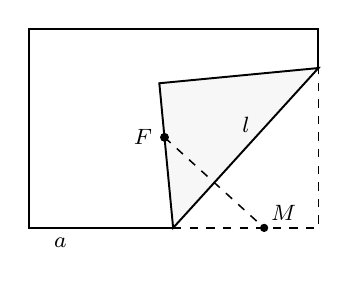
\begin{tikzpicture}[scale=1.15]
      % 矩形纸片范围: [0, 3.2] x [0, 2.2]
      % F = (1.5, 1.0), M = (2.6, 0)
      % 折痕 l 为 FM 的垂直平分线: 与 y=0 交于 A1=(1.5955, 0), 与 x=3.2 交于 A2=(3.2, 1.765)
      % 右下角 C=(3.2, 0) 关于 l 的对称点 C'=(1.443, 1.597)
      \coordinate (O) at (0,0);
      \coordinate (TL) at (0,2.2);
      \coordinate (TR) at (3.2,2.2);
      \coordinate (C) at (3.2,0);
      \coordinate (A1) at (1.5955,0);
      \coordinate (A2) at (3.2,1.765);
      \coordinate (Cp) at (1.443,1.597);
      \coordinate (F) at (1.5,1.0);
      \coordinate (M) at (2.6,0);

      % 原始纸片保留边
      \draw[line width=0.7pt] (A1) -- (O) -- (TL) -- (TR) -- (A2);
      % 原右下角虚线
      \draw[dashed, line width=0.6pt] (A1) -- (C) -- (A2);
      % 折起部分与折痕 l
      \draw[fill=gray!6, line width=0.7pt] (A1) -- (Cp) -- (A2) -- cycle;
      % 虚线 FM
      \draw[dashed, line width=0.55pt] (F) -- (M);

      % 标记点 F, M
      \fill (F) circle (1.4pt) node[left=1pt] {\footnotesize $F$};
      \fill (M) circle (1.3pt) node[above right=-1pt] {\footnotesize $M$};

      % 标注 a 与 l
      \node[below] at (0.35,0) {\footnotesize $a$};
      \node[above left] at (2.55,0.95) {\footnotesize $l$};
    \end{tikzpicture}
    \caption*{图\ 1.1}
  \end{minipage}
  \hfill
  \begin{minipage}[t]{0.47\textwidth}
    \centering
    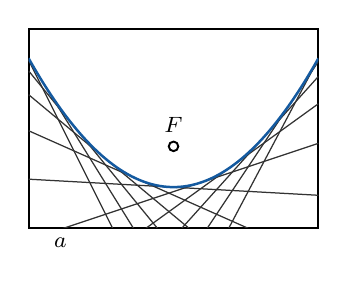
\begin{tikzpicture}[scale=1.15]
      % 矩形 [0, 3.2] x [0, 2.2], F=(1.6, 0.9), a: y=0
      \draw[line width=0.7pt] (0,0) rectangle (3.2,2.2);
      \begin{scope}
        \clip (0,0) rectangle (3.2,2.2);
        % 绘制若干折痕: 对 m in [-0.2, 3.4], y = ((m-1.6)/0.9)*(x - (m+1.6)/2) + 0.45
        \foreach \m in {-0.2, 0.15, 0.5, 0.85, 1.2, 1.55, 1.9, 2.25, 2.6, 2.95, 3.3} {
          \pgfmathsetmacro{\ya}{((\m-1.6)/0.9)*(0 - (\m+1.6)/2) + 0.45}
          \pgfmathsetmacro{\yb}{((\m-1.6)/0.9)*(3.2 - (\m+1.6)/2) + 0.45}
          \draw[line width=0.45pt, black!80] (0,\ya) -- (3.2,\yb);
        }
        % 抛物线包络: y = (x-1.6)^2 / 1.8 + 0.45
        \draw[line width=0.9pt, curveblue, domain=0:3.2, samples=80]
          plot (\x, {(\x-1.6)*(\x-1.6)/1.8 + 0.45});
      \end{scope}
      \draw[fill=white, line width=0.7pt] (1.6,0.9) circle (1.5pt);
      \node[above] at (1.6,0.94) {\footnotesize $F$};
      \node[below] at (0.35,0) {\footnotesize $a$};
    \end{tikzpicture}
    \caption*{图\ 1.2}
  \end{minipage}
\end{figure}

\begin{center}
  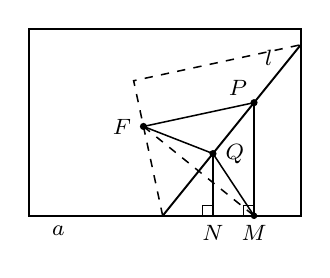
\begin{tikzpicture}[scale=1.08]
    % F = (1.35, 1.05), M = (2.65, 0)
    % 折痕 l 为 FM 中垂线: A1 = (1.57596, 0), A2 = (3.2, 2.01071)
    % 右下角 C = (3.2, 0) 关于 l 的精确对称点 C' = (1.23429, 1.58769)
    % 验证: A1, F, C' 严格共线, |A1 F| = |A1 M| = 1.07404, |F C'| = |M C| = 0.55
    \coordinate (O) at (0,0);
    \coordinate (TL) at (0,2.2);
    \coordinate (TR) at (3.2,2.2);
    \coordinate (C) at (3.2,0);
    \coordinate (A1) at (1.57596,0);
    \coordinate (A2) at (3.2,2.01071);
    \coordinate (Cp) at (1.23429,1.58769);
    \coordinate (F) at (1.35,1.05);
    \coordinate (M) at (2.65,0);
    \coordinate (P) at (2.65,1.32976);
    \coordinate (Q) at (2.167,0.7310);
    \coordinate (N) at (2.167,0);

    % 矩形纸片外框与折痕 l
    \draw[line width=0.7pt] (O) rectangle (TR);
    \draw[dashed, line width=0.55pt] (A1) -- (Cp) -- (A2);
    \draw[line width=0.7pt] (A1) -- (A2);

    % 辅助线段
    \draw[line width=0.55pt] (P) -- (M);
    \draw[line width=0.55pt] (Q) -- (N);
    \draw[dashed, line width=0.55pt] (F) -- (M);
    \draw[line width=0.55pt] (P) -- (F);
    \draw[line width=0.55pt] (Q) -- (F);
    \draw[line width=0.55pt] (Q) -- (M);

    % 直角符号
    \draw[line width=0.45pt] (M) ++(-0.12,0) -- ++(0,0.12) -- ++(0.12,0);
    \draw[line width=0.45pt] (N) ++(-0.12,0) -- ++(0,0.12) -- ++(0.12,0);

    % 点与标签
    \fill (F) circle (1.2pt) node[left=1pt] {\footnotesize $F$};
    \fill (P) circle (1.2pt) node[above left=-1pt] {\footnotesize $P$};
    \fill (Q) circle (1.2pt) node[right=1pt] {\footnotesize $Q$};
    \fill (M) circle (1.1pt) node[below] {\footnotesize $M$};
    \node[below] at (N) {\footnotesize $N$};
    \node[below] at (0.35,0) {\footnotesize $a$};
    \node[above left] at (2.98,1.65) {\footnotesize $l$};
  \end{tikzpicture}
  \par\vspace{4pt}{\footnotesize 图\ 1.3}
\end{center}

这种方法很有趣，要证明所得曲线确是抛物线也不难。如图 1.3，根据折法，直线 $a$ 上的点 $M$ 关于折痕 $l$ 与 $F$ 点对称。作 $MP \perp a$，交 $l$ 于 $P$；连 $PF$，则 $PF = PM$，即 $P$ 到定点 $F$ 的距离等于到定直线 $a$ 的距离，所以点 $P$ 在以 $F$ 为焦点、$a$ 为准线的抛物线上。其次，设 $Q$ 是 $l$ 上不同于 $P$ 的任意一点。连 $QF$、$QM$，作 $QN \perp a$，设垂足为 $N$，那么由直角三角形斜边大于直角边的性质，有
\[
  QF = QM > QN,
\]
总之，$QF \neq QN$，所以 $Q$ 点不在这条抛物线上。直线 $l$ 与这条抛物线有且只有一个公共点 $P$，并且由折纸方法知道 $l$ 不会垂直于 $a$，因而 $l$ 一定是这条抛物线的一条切线。同理，每条折痕都是这抛物线的一条切线。若干条折痕包围住同一条抛物线，就把这条抛物线的轮廓清楚地显示出来了。

\section{用折纸法画椭圆}
\markboth{2. 用折纸法画椭圆}{2. 用折纸法画椭圆}

上面一节使我们想到了抛物线的兄长——椭圆。椭圆是到两个定点的距离之和等于定长的点的轨迹。这两个定点叫做椭圆的焦点。

椭圆能不能用折纸法作出呢？也能。具体作法如下。

先用圆规在纸上画一个圆，小心地沿着圆周剪下一张圆形纸片来。设圆心是 $O$，在圆内任取一点 $F$（不能取 $O$），用笔在 $F$ 的位置做上记号。如图 2.1，把圆纸片翻起一角，使圆周正好通过 $F$，或者说使圆周上有一点 $M$ 落到 $F$ 的位置上，然后抹平纸片，得到一条折痕 $l$（为了看得清楚，也不妨用笔把直线 $l$ 描出来）。这样继续折下去，就得到若干条折痕。你会发现，这些折痕围出一个椭圆的轮廓（图 2.2）。画一条与这些折痕都相切的光滑曲线，就得到所要画的椭圆了。

\begin{center}
  \begin{minipage}[t]{0.47\textwidth}
    \centering
    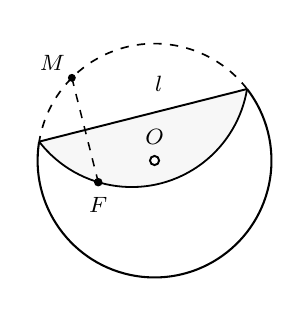
\begin{tikzpicture}[scale=1.1]
      % 圆心 O=(0,0), R=1.35, F=(-0.65, -0.25), M 在 135 度
      % 折痕 l 为 MF 的垂直平分线，交外圆于 A(170.695度), B(37.695度)
      \def\R{1.35}
      \coordinate (O) at (0,0);
      \coordinate (F) at (-0.65,-0.25);
      \coordinate (M) at ({\R*cos(135)},{\R*sin(135)});
      \coordinate (A) at ({\R*cos(170.695)},{\R*sin(170.695)});
      \coordinate (B) at ({\R*cos(37.695)},{\R*sin(37.695)});

      % 外圆周：保留部分为实线，A、B 之间被翻折走的左上圆弧为虚线
      \draw[line width=0.75pt] (A) arc[start angle=170.695, end angle=397.695, radius=\R];
      \draw[dashed, line width=0.6pt] (B) arc[start angle=37.695, end angle=170.695, radius=\R];
      % 折起弓形区域：浅灰背面填充（与图 1.1 一致）及折痕、翻折弧
      \fill[gray!6] (A) arc[start angle=-142.305, end angle=-9.305, radius=\R] -- (A) -- cycle;
      \draw[line width=0.7pt] (A) -- (B);
      \draw[line width=0.65pt] (A) arc[start angle=-142.305, end angle=-9.305, radius=\R];
      % 虚线 MF
      \draw[dashed, line width=0.55pt] (M) -- (F);

      % 标记点
      \draw[fill=white, line width=0.7pt] (O) circle (1.5pt) node[above=2pt] {\footnotesize $O$};
      \fill (F) circle (1.4pt) node[below=2pt] {\footnotesize $F$};
      \fill (M) circle (1.3pt) node[above left=-1pt] {\footnotesize $M$};
      \node[above] at (0.05,0.68) {\footnotesize $l$};
    \end{tikzpicture}
    \par\vspace{4pt}{\footnotesize 图\ 2.1}
  \end{minipage}
  \hfill
  \begin{minipage}[t]{0.47\textwidth}
    \centering
    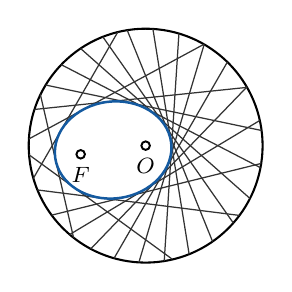
\begin{tikzpicture}[scale=1.1]
      \def\R{1.35}
      \coordinate (O) at (0,0);
      \coordinate (F) at (-0.75,-0.1);
      \draw[line width=0.75pt] (O) circle (\R);
      \begin{scope}
        \clip (O) circle (\R);
        \foreach \ang in {10, 30, 50, 70, 90, 110, 130, 150, 170, 190, 210, 230, 250, 270, 290, 310, 330, 350} {
          \pgfmathsetmacro{\mx}{\R*cos(\ang)}
          \pgfmathsetmacro{\my}{\R*sin(\ang)}
          \pgfmathsetmacro{\kx}{0.5*(\mx - 0.75)}
          \pgfmathsetmacro{\ky}{0.5*(\my - 0.1)}
          \pgfmathsetmacro{\dx}{-(\my + 0.1)}
          \pgfmathsetmacro{\dy}{\mx + 0.75}
          \draw[line width=0.45pt, black!80]
            (\kx - 2.2*\dx, \ky - 2.2*\dy) -- (\kx + 2.2*\dx, \ky + 2.2*\dy);
        }
      \end{scope}
      \draw[line width=0.9pt, curveblue, rotate around={7.595:(-0.375,-0.05)}]
        (-0.375,-0.05) ellipse [x radius=0.675, y radius=0.559];
      \draw[fill=white, line width=0.7pt] (O) circle (1.4pt) node[below=1pt] {\footnotesize $O$};
      \draw[fill=white, line width=0.7pt] (F) circle (1.4pt) node[below=1pt] {\footnotesize $F$};
    \end{tikzpicture}
    \par\vspace{4pt}{\footnotesize 图\ 2.2}
  \end{minipage}
\end{center}

为什么这样画出的曲线一定是椭圆呢？读者可以仿照上一节自己证证看。我们只是把证明需要的辅助图形画成图 2.3，并且告诉你 $F$ 与 $O$ 正是椭圆的焦点。

\begin{center}
  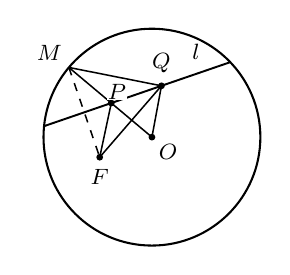
\begin{tikzpicture}[scale=1.02]
    \def\R{1.35}
    \coordinate (O) at (0,0);
    \coordinate (F) at (-0.65,-0.25);
    \coordinate (M) at ({1.35*cos(140)},{1.35*sin(140)});
    \coordinate (A) at (-1.3430, 0.1367);
    \coordinate (B) at (0.9752, 0.9333);
    \coordinate (P) at (-0.5059, 0.4245);
    \coordinate (Q) at (0.1187, 0.6390);

    \draw[line width=0.75pt] (O) circle (\R);
    \draw[line width=0.7pt] (A) -- (B);
    \draw[line width=0.55pt] (M) -- (O);
    \draw[dashed, line width=0.55pt] (M) -- (F);
    \draw[line width=0.55pt] (P) -- (F);
    \draw[line width=0.55pt] (Q) -- (F);
    \draw[line width=0.55pt] (Q) -- (M);
    \draw[line width=0.55pt] (Q) -- (O);

    \fill (F) circle (1.2pt) node[below=1pt] {\footnotesize $F$};
    \fill (O) circle (1.2pt) node[below right=-1pt] {\footnotesize $O$};
    \fill (P) circle (1.2pt);
    \node[fill=white, inner sep=0.4pt] at ($(P)+(0.07,0.14)$) {\footnotesize $P$};
    \fill (Q) circle (1.2pt) node[above=1pt] {\footnotesize $Q$};
    \node[above left=-1pt] at (M) {\footnotesize $M$};
    \node[above] at (0.55,0.85) {\footnotesize $l$};
  \end{tikzpicture}
  \par\vspace{4pt}{\footnotesize 图\ 2.3}
\end{center}

\section{百发百中}
\markboth{3. 百发百中}{3. 百发百中}

人们常用“百发百中”来赞美神枪手。但是我们这里说的“百发百中”，却是指一个有趣的小游戏。

如图 3.1，用硬纸做一个椭圆形的盒子，并且在椭圆形盒底的一个焦点上放一粒钮扣，作为子弹，在另一个焦点处竖立一个钢笔套，作为靶子。你不需要瞄准，把钮扣子弹沿着盒底面内的任何方向弹射出去，经过盒壁反射后，都一定命中靶子，真是不折不扣的百发百中呢！

\begin{center}
  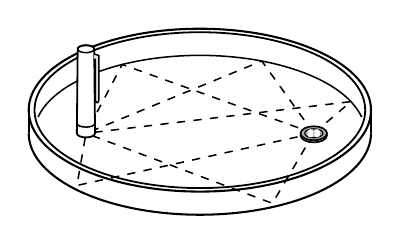
\begin{tikzpicture}[scale=1.05]
    % 椭圆形硬纸盒斜投影: 内底半轴 a=2.0, b=0.9425, 焦点 F1=(-1.3775, 0), F2=(1.3775, 0)
    \def\a{2.0}
    \def\b{0.9425}
    \def\c{1.3775}
    \def\h{0.28}

    % 盒外壁底部可见弧与两侧垂线
    \draw[line width=0.75pt] (-2.07,0) arc[start angle=180, end angle=360, x radius=2.07, y radius=0.985];
    \draw[line width=0.75pt] (-2.07,0) -- (-2.07,\h);
    \draw[line width=0.75pt] (2.07,0) -- (2.07,\h);
    % 盒顶外沿与内沿
    \draw[line width=0.75pt, fill=white] (0,\h) ellipse [x radius=2.07, y radius=0.985];
    \draw[line width=0.65pt, fill=white] (0,\h) ellipse [x radius=\a, y radius=\b];
    % 盒内壁底面可见弧(后半弧)
    \draw[line width=0.55pt] ({\a*cos(12)},{\b*sin(12)}) arc[start angle=12, end angle=168, x radius=\a, y radius=\b];

    \coordinate (F1) at (-\c, 0);
    \coordinate (F2) at (\c, 0);

    % 精确椭圆反射路径: 从 F2 射向盒底内壁 W(t), 反射至 F1
    \foreach \t in {24, 68, 118, 222, 296} {
      \coordinate (W) at ({\a*cos(\t)}, {\b*sin(\t)});
      \draw[dashed, line width=0.55pt] (F2) -- (W) -- (F1);
    }

    % 焦点 F2 处的四孔钮扣
    \begin{scope}[shift={(F2)}]
      \draw[fill=gray!25, line width=0.6pt] (0,-0.025) ellipse [x radius=0.16, y radius=0.085];
      \draw[fill=gray!65, line width=0.6pt] (0,0) ellipse [x radius=0.16, y radius=0.085];
      \draw[line width=0.4pt] (0,0) ellipse [x radius=0.11, y radius=0.055];
      \fill[white] (-0.04,0.015) circle (1.0pt) (0.04,0.015) circle (1.0pt)
                   (-0.04,-0.015) circle (1.0pt) (0.04,-0.015) circle (1.0pt);
    \end{scope}

    % 焦点 F1 处竖立的钢笔套(带笔夹)
    \begin{scope}[shift={(F1)}]
      \draw[fill=white, line width=0.65pt]
        (-0.11,0) arc[start angle=180, end angle=360, x radius=0.11, y radius=0.05]
        -- (0.10,1.02) arc[start angle=0, end angle=180, x radius=0.10, y radius=0.045]
        -- cycle;
      \draw[line width=0.55pt] (0,1.02) ellipse [x radius=0.10, y radius=0.045];
      \draw[line width=0.55pt] (-0.108,0.12) arc[start angle=180, end angle=360, x radius=0.108, y radius=0.045];
      \draw[fill=gray!20, line width=0.55pt]
        (0.10,0.96) -- (0.155,0.94) -- (0.155,0.40) arc[start angle=0, end angle=-180, x radius=0.02, y radius=0.03] -- (0.115,0.89) -- (0.10,0.90);
    \end{scope}
  \end{tikzpicture}
  \par\vspace{4pt}{\footnotesize 图\ 3.1}
\end{center}

\begin{wrapfigure}{r}{0.43\textwidth}
  \centering
  \vspace{-6pt}
  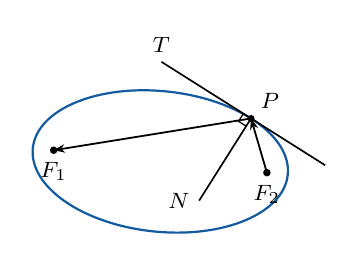
\begin{tikzpicture}[scale=1.05]
    \begin{scope}[rotate=-6]
      \def\a{1.55}
      \def\b{0.85}
      \def\c{1.2961}
      \coordinate (F1) at (-\c,0);
      \coordinate (F2) at (\c,0);
      \coordinate (P) at ({\a*cos(48)},{\b*sin(48)});
      \coordinate (T) at ($(P) + (-1.15, 0.568)$);
      \coordinate (TR) at ($(P) + (0.95, -0.469)$);
      \coordinate (N) at ($(P) + (-0.52, -1.053)$);

      \draw[line width=0.8pt, curveblue] (0,0) ellipse [x radius=\a, y radius=\b];
      \draw[line width=0.6pt] (T) -- (TR);
      \draw[line width=0.6pt] (P) -- (N);
      \draw[line width=0.65pt, -{Stealth[length=4pt]}] (F2) -- (P);
      \draw[line width=0.65pt, -{Stealth[length=4pt]}] (P) -- (F1);

      % 切线与法线的直角标志
      \coordinate (uT) at (-0.8966, 0.4428);
      \coordinate (uN) at (-0.4428, -0.8966);
      \draw[line width=0.45pt] ($(P) + 0.11*(uT)$) -- ($(P) + 0.11*(uT) + 0.11*(uN)$) -- ($(P) + 0.11*(uN)$);

      \fill (F1) circle (1.3pt) node[below=1pt] {\footnotesize $F_1$};
      \fill (F2) circle (1.3pt) node[below=1pt] {\footnotesize $F_2$};
      \fill (P) circle (1.2pt) node[above right=0pt] {\footnotesize $P$};
      \node[above] at (T) {\footnotesize $T$};
      \node[left] at (N) {\footnotesize $N$};
    \end{scope}
  \end{tikzpicture}
  \caption*{图\ 3.2}
  \vspace{-6pt}
\end{wrapfigure}

这个游戏的原理，在物理方面是利用了反射定律，在数学方面是利用了椭圆的切线和法线的性质。反射定律告诉我们，当一束光线被平面镜反射时，反射光线与镜面法线的夹角（反射角），总是等于入射光线与法线的夹角（入射角）。当反射镜的表面形状是曲面时，可以把一小块曲面近似地当成一小块平面，因而“反射角等于入射角”这一定律仍然适用。现在我们的盒底是椭圆形的，而椭圆的法线有一个特殊的性质：若 $P$ 是椭圆上的任意点，$F_1$ 和 $F_2$ 是两个焦点，则法线 $PN$ 平分 $\angle F_1PF_2$（图 3.2）。因此，如果有一束光线沿 $F_2P$ 方向射到椭圆上，经反射后一定沿 $PF_1$ 方向射出。$P$ 是椭圆上的任意点，所以从一个焦点 $F_2$ 沿任何方向射出的光线，经过椭圆反射后都通过另一个焦点 $F_1$。把射出光线换成射出钮扣，经过椭圆盒壁反射后，那当然总是会击中放在另一个焦点 $F_1$ 处的钢笔套啦。

\section{双曲线为摄影师帮忙}
\markboth{4. 双曲线为摄影师帮忙}{4. 双曲线为摄影师帮忙}

\noindent
\begin{minipage}[t]{0.53\textwidth}
  \setlength{\parindent}{2em}
  现在该来谈谈双曲线了。双曲线是到两个定点的距离之差等于定长的点的轨迹。这两个定点叫做双曲线的焦点。把双曲线绕着两个焦点的连线在空间旋转一周，所得到的曲面叫做双叶旋转双曲面。有一种灯具的反射镜的表面就是做成这种曲面的形状（如图 4.1）。这种镜面有一个特点，把光源放在一个焦点上，那么它所发出的光线经过镜面反射以后，好像都是从另一个焦点发出来似的。
\end{minipage}
\hfill
\begin{minipage}[t]{0.44\textwidth}
  \centering
  \vspace{-2pt}
  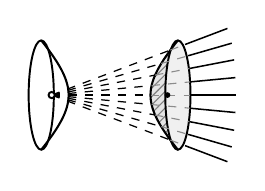
\begin{tikzpicture}[scale=0.80]
    % 双叶旋转双曲面反射镜: a=0.65, b=0.65, c=0.9192, t in [-1.1, 1.1]
    % 右叶顶点 (0.65, 0), 左叶顶点 (-0.65, 0)
    % 虚焦点 F1=(-0.9192, 0), 实光源焦点 F2=(0.9192, 0)
    % 开口位置 x_rim = 0.65*cosh(1.1) = 1.0845, y_rim = 0.65*sinh(1.1) = 0.8682
    \def\a{0.65}
    \def\b{0.65}
    \def\c{0.9192}

    % 右叶金属外壳阴影(左叶侧视外表面)与开口凹面内壁
    \fill[black!10]
      plot[domain=-1.1:1.1, samples=40] ({\a*cosh(\x)}, {\b*sinh(\x)})
      -- (1.0845, -0.8682) arc[start angle=-90, end angle=90, x radius=0.20, y radius=0.8682]
      -- cycle;
    \fill[pattern=north east lines, pattern color=black!50]
      plot[domain=-1.1:1.1, samples=40] ({\a*cosh(\x)}, {\b*sinh(\x)})
      arc[start angle=90, end angle=270, x radius=0.20, y radius=0.8682]
      -- cycle;
    \fill[black!6] (1.0845,0) ellipse [x radius=0.20, y radius=0.8682];
    \draw[line width=0.75pt]
      plot[domain=-1.1:1.1, samples=40] ({\a*cosh(\x)}, {\b*sinh(\x)});
    \draw[line width=0.7pt] (1.0845,0) ellipse [x radius=0.20, y radius=0.8682];

    % 左叶轮廓
    \draw[line width=0.75pt]
      plot[domain=-1.1:1.1, samples=40] ({-\a*cosh(\x)}, {\b*sinh(\x)});
    \draw[line width=0.7pt] (-1.0845,0) ellipse [x radius=0.20, y radius=0.8682];

    % 从左焦点 F1 出发的反向延长虚线止于右叶轮廓, 实线光线从右叶开口端净射出(不穿透镜背)
    \coordinate (F1) at (-\c, 0);
    \foreach \t in {-0.95, -0.71, -0.47, -0.23, 0, 0.23, 0.47, 0.71, 0.95} {
      \pgfmathsetmacro{\px}{\a*cosh(\t)}
      \pgfmathsetmacro{\py}{\b*sinh(\t)}
      \pgfmathsetmacro{\vx}{\px + \c}
      \pgfmathsetmacro{\vy}{\py}
      \pgfmathsetmacro{\len}{sqrt(\vx*\vx + \vy*\vy)}
      \pgfmathsetmacro{\ux}{\vx/\len}
      \pgfmathsetmacro{\uy}{\vy/\len}
      % 出射光线穿过开口椭圆右半缘(近似截断到开口外侧, 避免穿过实体镜背阴影)
      \pgfmathsetmacro{\kexit}{max(0, (1.0845 + 0.20*sqrt(max(0, 1 - (\py/0.8682)*(\py/0.8682))) - \px)/\ux)}
      \pgfmathsetmacro{\ex}{\px + \kexit*\ux}
      \pgfmathsetmacro{\ey}{\py + \kexit*\uy}
      \draw[dashed, line width=0.45pt] (F1) -- (\px, \py);
      \draw[dashed, line width=0.4pt, black!45] (\px, \py) -- (\ex, \ey);
      \draw[line width=0.55pt] (\ex, \ey) -- ({\px + (\kexit + 0.72)*\ux}, {\py + (\kexit + 0.72)*\uy});
    }
    % 左焦点(虚焦点)与右焦点(灯丝位置)小圆圈
    \draw[fill=white, line width=0.7pt] (F1) circle (1.4pt);
    \fill[black] (\c, 0) circle (1.3pt);
  \end{tikzpicture}
  \par\vspace{4pt}{\footnotesize 图\ 4.1}
\end{minipage}

这样做出的灯具有什么好处呢？原来在室内拍照片时，由于自然光线不足，常常需要借助闪光灯或其它照明灯具。为了把被摄对象照得更亮，摄影师总想把灯尽可能放近些。但是一般自然光线接近于平行光线，因而均匀柔和；而灯光则是中心放射式的，灯放得越近，光线的放射性效应越明显。为了既获得足够的亮度，又使光线尽量地均匀柔和，专门为摄影师设计的照明灯，就往往利用双曲线的光学性质，把反光镜的表面做成双叶旋转双曲面的形状，并让灯丝恰好位于焦点。

\section{让光线多跑两趟}
\markboth{5. 让光线多跑两趟}{5. 让光线多跑两趟}

\noindent
\begin{minipage}[t]{0.46\textwidth}
  \centering
  \vspace{-2pt}
  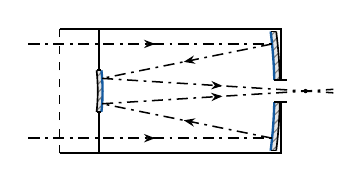
\begin{tikzpicture}[scale=0.88]
    % 镜筒范围 x in [0, 3.2], y in [-0.9, 0.9]
    % 抛物线主镜: x = 3.1 - y^2/13.6, F1 = (-0.3, 0)
    % 双曲线副镜: F1=(-0.3,0), F2=(3.55,0), a=1.005, c=1.925, b^2=2.6956

    % 镜筒外壁(筒底紧贴主镜小洞外框, 无断开空隙)
    \draw[line width=0.75pt] (0,0.9) -- (3.20,0.9) -- (3.20,0.16) -- (3.28,0.16);
    \draw[line width=0.75pt] (0,-0.9) -- (3.20,-0.9) -- (3.20,-0.16) -- (3.28,-0.16);
    \draw[dashed, line width=0.5pt] (0,-0.9) -- (0,0.9);

    % 抛物线主镜(实心玻璃体+镜背斜线阴影, 上下两半, 中间留小洞 |y| < 0.16)
    \fill[black!10]
      plot[domain=0.16:0.86, samples=25] ({3.1 - \x*\x/13.6}, \x)
      -- plot[domain=0.86:0.16, samples=25] ({3.18 - \x*\x/13.6}, \x) -- cycle;
    \fill[pattern=north east lines, pattern color=black!50]
      plot[domain=0.16:0.86, samples=25] ({3.1 - \x*\x/13.6}, \x)
      -- plot[domain=0.86:0.16, samples=25] ({3.18 - \x*\x/13.6}, \x) -- cycle;
    \fill[black!10]
      plot[domain=-0.86:-0.16, samples=25] ({3.1 - \x*\x/13.6}, \x)
      -- plot[domain=-0.16:-0.86, samples=25] ({3.18 - \x*\x/13.6}, \x) -- cycle;
    \fill[pattern=north east lines, pattern color=black!50]
      plot[domain=-0.86:-0.16, samples=25] ({3.1 - \x*\x/13.6}, \x)
      -- plot[domain=-0.16:-0.86, samples=25] ({3.18 - \x*\x/13.6}, \x) -- cycle;

    \draw[line width=0.85pt, curveblue, domain=0.16:0.86, samples=25]
      plot ({3.1 - \x*\x/13.6}, \x);
    \draw[line width=0.85pt, curveblue, domain=-0.86:-0.16, samples=25]
      plot ({3.1 - \x*\x/13.6}, \x);
    \draw[line width=0.6pt, domain=0.16:0.86, samples=25]
      plot ({3.18 - \x*\x/13.6}, \x);
    \draw[line width=0.6pt, domain=-0.86:-0.16, samples=25]
      plot ({3.18 - \x*\x/13.6}, \x);
    \draw[line width=0.6pt] ({3.1-0.86*0.86/13.6},0.86) -- ({3.18-0.86*0.86/13.6},0.86);
    \draw[line width=0.6pt] ({3.1-0.16*0.16/13.6},0.16) -- (3.20,0.16);
    \draw[line width=0.6pt] ({3.1-0.86*0.86/13.6},-0.86) -- ({3.18-0.86*0.86/13.6},-0.86);
    \draw[line width=0.6pt] ({3.1-0.16*0.16/13.6},-0.16) -- (3.20,-0.16);

    % 双曲线副镜(实心反射镜+背面支杆止于镜缘, 不穿透镜体)
    \fill[black!10]
      plot[domain=-0.30:0.30, samples=25] ({1.625 - 1.005*sqrt(1 + \x*\x/2.6956)}, \x)
      -- plot[domain=0.30:-0.30, samples=25] ({1.555 - 1.005*sqrt(1 + \x*\x/2.6956)}, \x) -- cycle;
    \fill[pattern=north east lines, pattern color=black!50]
      plot[domain=-0.30:0.30, samples=25] ({1.625 - 1.005*sqrt(1 + \x*\x/2.6956)}, \x)
      -- plot[domain=0.30:-0.30, samples=25] ({1.555 - 1.005*sqrt(1 + \x*\x/2.6956)}, \x) -- cycle;
    \draw[line width=0.85pt, curveblue, domain=-0.30:0.30, samples=25]
      plot ({1.625 - 1.005*sqrt(1 + \x*\x/2.6956)}, \x);
    \draw[line width=0.6pt, domain=-0.30:0.30, samples=25]
      plot ({1.555 - 1.005*sqrt(1 + \x*\x/2.6956)}, \x);
    \pgfmathsetmacro{\secFrontX}{1.625 - 1.005*sqrt(1 + 0.09/2.6956)}
    \pgfmathsetmacro{\secBackX}{1.555 - 1.005*sqrt(1 + 0.09/2.6956)}
    \pgfmathsetmacro{\secMidX}{0.5*(\secFrontX + \secBackX)}
    \draw[line width=0.6pt] (\secFrontX,0.30) -- (\secBackX,0.30);
    \draw[line width=0.6pt] (\secFrontX,-0.30) -- (\secBackX,-0.30);
    \draw[line width=0.5pt] (\secMidX,0.30) -- (\secMidX,0.9);
    \draw[line width=0.5pt] (\secMidX,-0.30) -- (\secMidX,-0.9);

    % 光学路径
    \coordinate (InT) at (-0.45, 0.68);
    \coordinate (InB) at (-0.45, -0.68);
    \coordinate (P1T) at (3.066, 0.68);
    \coordinate (P1B) at (3.066, -0.68);
    \coordinate (P2T) at (0.614, 0.183);
    \coordinate (P2B) at (0.614, -0.183);
    \coordinate (OutT) at (3.95, -0.025);
    \coordinate (OutB) at (3.95, 0.025);

    \begin{scope}[
      dash pattern=on 4pt off 2pt on 1pt off 2pt,
      line width=0.55pt,
      decoration={markings, mark=at position 0.52 with {\arrow{Stealth[length=4pt]}}}
    ]
      \draw[postaction={decorate}] (InT) -- (P1T);
      \draw[postaction={decorate}] (InB) -- (P1B);
      \draw[postaction={decorate}] (P1T) -- (P2T);
      \draw[postaction={decorate}] (P1B) -- (P2B);
      \draw[postaction={decorate}] (P2T) -- (OutT);
      \draw[postaction={decorate}] (P2B) -- (OutB);
    \end{scope}

    % 聚焦处加注清晰会聚交点(去除空白遮挡椭圆)
    \fill (3.55,0) circle (0.9pt);
  \end{tikzpicture}
  \par\vspace{4pt}{\footnotesize 图\ 5.1}
\end{minipage}
\hfill
\begin{minipage}[t]{0.51\textwidth}
  \setlength{\parindent}{2em}
  1672 年，卡塞格林发明了一种天文望远镜，这种望远镜巧妙地利用了曲线的性质，被人们叫做卡塞格林反射式天文望远镜。图 5.1 就是这种望远镜的示意图。
\end{minipage}

图中的矩形边框表示望远镜的镜筒，左边是筒口，右边是筒底。紧靠筒底的曲线表示一面口径很大的反射镜，它的截面是抛物线弧。大反射镜的正中有一个小洞，和筒底正中的小窗口连在一起。左边靠近筒口的地方还有一面较小的反射镜，小反射镜的截面是双曲线弧，并且双曲线的一个焦点恰好与抛物线的焦点重合，双曲线的另一个焦点在镜筒底部中心的小窗附近。

这种望远镜的工作原理是这样的：假定图 5.1 中的点划线表示光线，箭头表示光线前进的方向。来自遥远星空的平行光线，进入卡塞格林望远镜的镜筒以后，直奔筒底，在那里受到抛物线大反射镜的反射，掉转头来，朝着筒口方向，对准抛物线的焦点射去。在到达目的地之前，就已遇到拦路的双曲线小反射镜。由于这些光线的投射目标恰好也是双曲线的一个焦点，所以在小反射镜的反射之下，这些光线转身重新射向镜筒底部，并且对准双曲线的第二个焦点射去（为什么？读者自己想一想），在那里聚焦成像。而成象处附近正是镜筒底部的小窗口，所以在镜筒后面的观测者可以透过目镜观测到天空的景象。

卡塞格林反射式天文望远镜最巧妙的地方，在于它把抛物线和双曲线组合起来，让进入镜筒的光线在聚焦过程中往返奔波，多跑两趟，因而镜筒的长度比光线实际走过的路程短得多，这样就能使仪器的体积缩小，重量减轻，既经济，又方便。所以，在现代的激光雷达和无线电接收装置中也都很喜欢采用卡塞格林的反射系统。

\section{杰尼西亚的耳朵}
\markboth{6. 杰尼西亚的耳朵}{6. 杰尼西亚的耳朵}

\noindent
\begin{minipage}[t]{0.55\textwidth}
  \setlength{\parindent}{2em}
  据传说，在意大利西西里岛有一个山洞，很久以前，叙拉古的暴君杰尼西亚把他的一些囚犯关在这个山洞里。囚犯们多次密谋逃跑，但是每次的计划都被杰尼西亚发现了。起初，囚犯们怀疑自己的同伴中有内奸，他们彼此指责，互相猜疑，但是始终没有发现任何一个囚犯告密。后来渐渐觉察到囚禁他们的山洞形状古怪，洞壁把囚犯们的话都反射到狱卒的耳朵里去了，囚犯们诅咒这个山洞是“杰尼西亚的耳朵”。从图 6.1 可以看出，山洞的剖面近似于椭圆，犯人聚居的地方恰好在一个焦点附近，狱卒在另一个焦点偷听，无论囚犯们怎样压低嗓门，他们的声音照样被狱卒偷听得清清楚楚。
\end{minipage}
\hfill
\begin{minipage}[t]{0.42\textwidth}
  \centering
  \vspace{-2pt}
  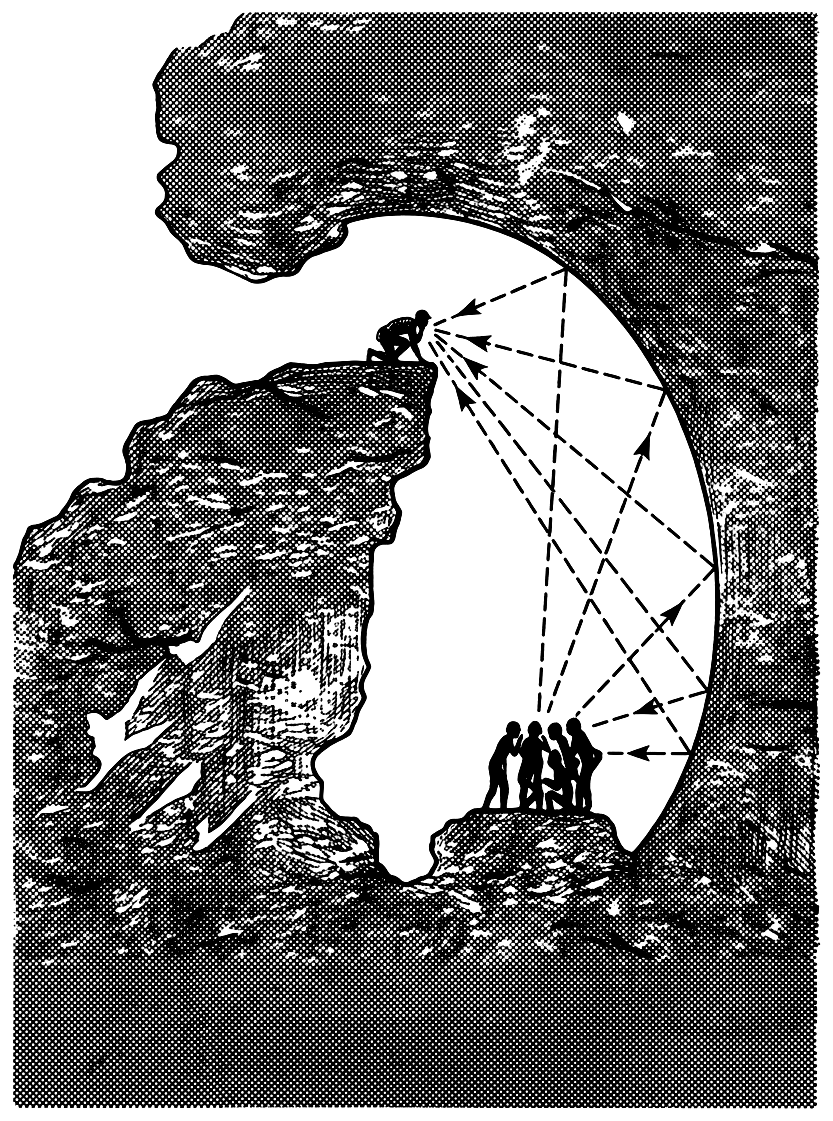
\includegraphics[width=\linewidth]{fig_006_1.png}
  \par\vspace{4pt}{\footnotesize 图\ 6.1}
\end{minipage}

这个传说表明，椭圆形的反射面不但能使从一个焦点发出的光线在另一个焦点会聚，而且能使从一个焦点发出的声音在另一个焦点聚焦。人们曾经发现一个古希腊音乐厅的墙壁正是椭圆形的，乐池位于一个焦点附近。在这个音乐厅里，乐队演奏的声音会在另一个焦点重新会聚起来。美国有一个教堂也有类似的设计，这种设计的出发点不得而知，其实声音的聚焦并不是好事，因为在另一焦点附近的听众固然连演奏或演讲者的细声慢语都能听见；但是在室内其它地方，音响效果却差得多。因而，现代在设计音乐厅、影剧院、大会堂等大型建筑物时，建筑设计人员都很注意设法避免声聚焦。

\section{抛物线与屋顶}
\markboth{7. 抛物线与屋顶}{7. 抛物线与屋顶}

\noindent
\begin{minipage}[t]{0.43\textwidth}
  \centering
  \vspace{-2pt}
  \begin{tikzpicture}[scale=0.76]
    \def\px#1#2{1.0*(#1) + 0.85*(#2)}
    \def\py#1#2{0.22*(#1) - 0.48*(#2) - 0.35*(#1)*(#1) - 0.25*(#2)*(#2)}

    \draw[line width=0.65pt]
      plot[domain=-1:1, samples=25] ({\px{-1}{\x}}, {\py{-1}{\x}});
    \draw[line width=0.65pt]
      plot[domain=-1:1, samples=25] ({\px{1}{\x}}, {\py{1}{\x}});
    \foreach \vv in {-1, 0, 1} {
      \draw[line width=0.7pt, curveblue, domain=-1:1, samples=30]
        plot ({\px{\x}{\vv}}, {\py{\x}{\vv}});
      \draw[line width=0.5pt] ({\px{-1}{\vv}}, {\py{-1}{\vv}}) -- ({\px{1}{\vv}}, {\py{1}{\vv}});
    }
    \node[below, font=\scriptsize] at ({\px{-0.30}{-1}}, {\py{-0.30}{-1}-0.02}) {$a$};
    \node[below, font=\scriptsize] at ({\px{-0.32}{0}}, {\py{-0.32}{0}-0.03}) {$a$};
    \node[below, font=\scriptsize] at ({\px{0.35}{1}}, {\py{0.35}{1}-0.05}) {$a$};
    \draw[line width=0.85pt, black, domain=-1:1, samples=30]
      plot ({\px{0}{\x}}, {\py{0}{\x}});
    \node[above right=-2pt, font=\scriptsize] at ({\px{0}{-0.20}}, {\py{0}{-0.20}}) {$b$};

    \draw[-{Stealth[length=5pt]}, line width=1.4pt]
      (-0.9, 0.65) .. controls (-0.1, 0.95) and (0.55, 0.65) .. (1.05, 0.12);
    \node[above, font=\scriptsize] at (0.12, 0.86) {曲线 $a$ 沿曲线 $b$ 平行移动};
  \end{tikzpicture}
  \par\vspace{4pt}{\footnotesize 图\ 7.1}
\end{minipage}
\hfill
\begin{minipage}[t]{0.53\textwidth}
  \setlength{\parindent}{2em}
  如图 7.1，一条曲线 $a$ 可以沿着另一条曲线 $b$ 平行移动（即在移动过程中曲线 $a$ 上任意两点的连线与初始位置平行）。一条曲线沿着另一曲线平行移动所产生的曲面，叫做平移曲面。
\end{minipage}

\medskip
\noindent
\begin{minipage}[t]{0.53\textwidth}
  \setlength{\parindent}{2em}
  在图 7.1 中，动曲线 $a$ 是开口向下的抛物线，定曲线 $b$ 也是开口向下的抛物线，这样得到的平移曲面叫做椭圆抛物面。而在图 7.2 中，动曲线 $a$ 仍是开口向下的抛物线，定曲线 $b$ 却是开口向上的抛物线，这样得到的平移曲面叫做双曲抛物面。双曲抛物面又叫马鞍面，因为它的形状有点像马鞍。
\end{minipage}
\hfill
\begin{minipage}[t]{0.44\textwidth}
  \centering
  \vspace{-2pt}
  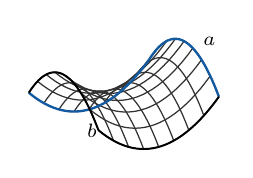
\begin{tikzpicture}[scale=0.85]
    \def\sx#1#2{0.90*(#2) - 0.52*(#1)}
    \def\sy#1#2{0.25*(#2) + 0.28*(#1) + 0.50*(#2)*(#2) - 0.55*(#1)*(#1)}

    \foreach \uu in {-1, -0.75, -0.5, -0.25, 0, 0.25, 0.5, 0.75, 1} {
      \draw[line width=0.45pt, black!80, domain=-1:1, samples=25]
        plot ({\sx{\uu}{\x}}, {\sy{\uu}{\x}});
    }
    \foreach \vv in {-1, -0.75, -0.5, -0.25, 0, 0.25, 0.5, 0.75, 1} {
      \draw[line width=0.45pt, black!80, domain=-1:1, samples=25]
        plot ({\sx{\x}{\vv}}, {\sy{\x}{\vv}});
    }
    \draw[line width=0.85pt, curveblue, domain=-1:1, samples=30]
      plot ({\sx{\x}{1}}, {\sy{\x}{1}});
    \draw[line width=0.85pt, curveblue, domain=-1:1, samples=30]
      plot ({\sx{1}{\x}}, {\sy{1}{\x}});
    \draw[line width=0.7pt, domain=-1:1, samples=30]
      plot ({\sx{\x}{-1}}, {\sy{\x}{-1}});
    \draw[line width=0.7pt, domain=-1:1, samples=30]
      plot ({\sx{-1}{\x}}, {\sy{-1}{\x}});

    \node[above right=-1pt, font=\scriptsize] at ({\sx{-0.35}{1}}, {\sy{-0.35}{1}}) {$a$};
    \node[below=2pt, font=\scriptsize] at ({\sx{1}{0.05}}, {\sy{1}{0.05}}) {$b$};
  \end{tikzpicture}
  \par\vspace{4pt}{\footnotesize 图\ 7.2}
\end{minipage}

由抛物线产生的平移曲面，常被应用到一些建筑物的屋顶上。例如北京网球馆的屋面形状是椭圆抛物面（图 7.3），而北京火车站的屋顶上有六处做成椭圆抛物面的形状（图 7.4）。这些椭圆抛物面的屋顶看上去形状有点像球面，因而大方匀称。但在实际施工时，浇制椭圆抛物面的屋顶要比浇制球面方便。这是因为预制水泥构件时要先做模板，而用一组平行平面去截球面，截面圆的半径是变化的，所以浇制球面时各块模板的形状互不相同，要做多块模板。而椭圆抛物面或双曲抛物面由于是平移曲面，所以浇制时每块模板的形状和大小都是完全相同的抛物线，这样就方便多了。

\begin{figure}[htbp]
  \centering
  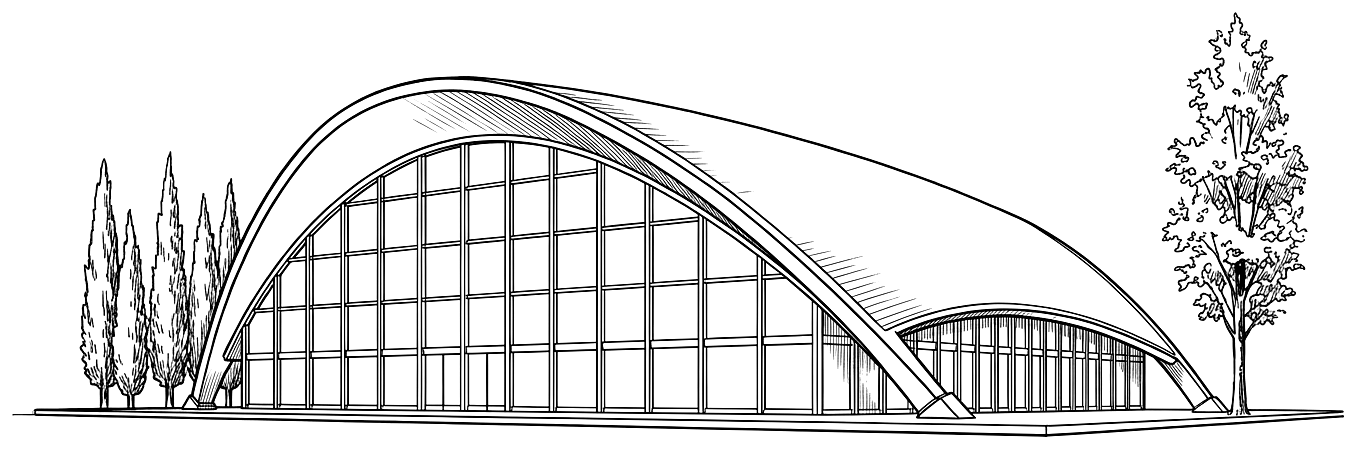
\includegraphics[width=0.78\textwidth]{fig_007_3.png}
  \caption*{图\ 7.3}
\end{figure}

\begin{figure}[htbp]
  \centering
  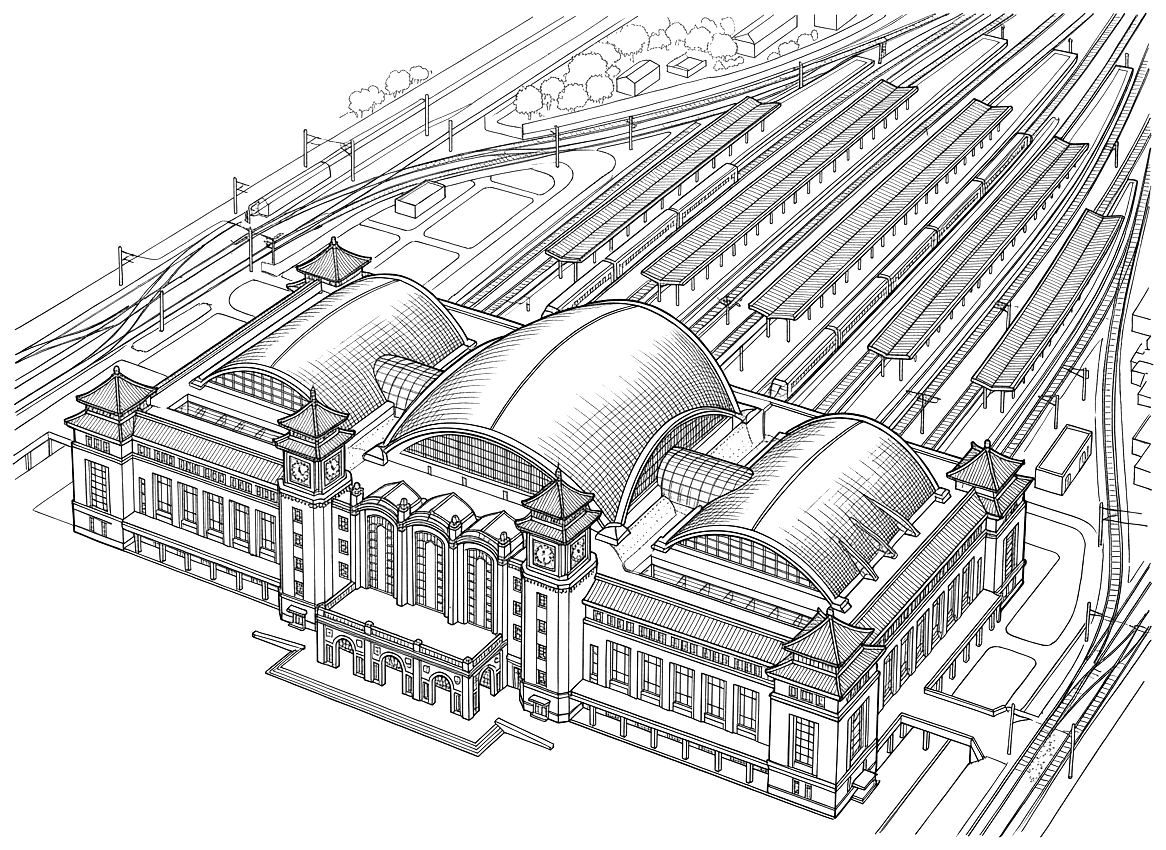
\includegraphics[width=0.78\textwidth]{fig_007_4.png}
  \caption*{图\ 7.4}
\end{figure}

\section{用三角板画抛物线}
\markboth{8. 用三角板画抛物线}{8. 用三角板画抛物线}

抛物线也可利用三角板来画，其方法既有趣，又实用。如图 8.1，取一点 $F$，并且作一条不通过 $F$ 的直线 $a$。让三角板的一条直角边 $LM$ 通过定点 $F$，直角顶点 $M$ 放在直线 $a$ 上的任一位置，然后沿另一条直角边 $MN$ 画直线，就得到所要作的抛物线的一条切线。用同样方法再画出若干条直线，最后再画一条与这些直线都相切的光滑曲线，就得到了所要画的抛物线。

\begin{figure}[htbp]
  \centering
  \begin{minipage}[t]{0.47\textwidth}
    \centering
    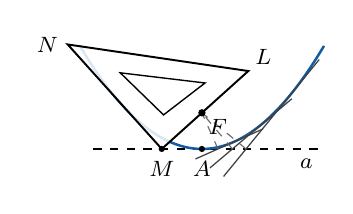
\begin{tikzpicture}[scale=1.02]
      % 抛物线 y = x^2 / 1.8, 顶点 A=(0,0), 焦点 F=(0, 0.45), 直线 a: y=0
      \coordinate (A) at (0,0);
      \coordinate (F) at (0,0.45);
      % 直线 a
      \draw[dashed, line width=0.65pt] (-1.35,0) -- (1.45,0);
      \node[below] at (1.30,0) {\footnotesize $a$};
      % 抛物线
      \draw[line width=0.9pt, curveblue, domain=-1.52:1.52, samples=70]
        plot (\x, {\x*\x/1.8});
      % 右侧几条切线: 在 a 上取 M=(m,0), 切点 P=(2m, 2m^2/0.9) = (2m, 4m^2/1.8)
      % 斜率为 2m/0.9 = m/0.45, 方程 y = (m/0.45)*(x - m)
      \foreach \m in {0.20, 0.38, 0.55} {
        \draw[line width=0.45pt, black!75] (\m-0.28, {(\m/0.45)*(-0.28)}) -- (2*\m+0.36, {(\m/0.45)*(\m+0.36)});
        \draw[line width=0.4pt, dashed, black!60] (\m,0) -- (F);
      }
      % 三角板: 直角顶点 M=(-0.50, 0), F=(0, 0.45)
      % MF 方向 (0.50, 0.45), 单位化 (0.7433, 0.6690)
      % 垂直方向 (-0.6690, 0.7433)
      \coordinate (M) at (-0.50, 0);
      \coordinate (L) at ($(M) + 1.45*(0.7433, 0.6690)$);
      \coordinate (N) at ($(M) + 1.75*(-0.6690, 0.7433)$);
      \draw[line width=0.7pt, fill=white, fill opacity=0.85] (M) -- (L) -- (N) -- cycle;
      % 三角板内部镂空三角形
      \coordinate (M1) at ($(M) + 0.30*(0.7433, 0.6690) + 0.30*(-0.6690, 0.7433)$);
      \coordinate (L1) at ($(M) + 0.95*(0.7433, 0.6690) + 0.25*(-0.6690, 0.7433)$);
      \coordinate (N1) at ($(M) + 0.25*(0.7433, 0.6690) + 1.05*(-0.6690, 0.7433)$);
      \draw[line width=0.5pt] (M1) -- (L1) -- (N1) -- cycle;

      % 标记点
      \fill (F) circle (1.3pt) node[below right=-1pt] {\footnotesize $F$};
      \fill (A) circle (1.1pt) node[below=1pt] {\footnotesize $A$};
      \fill (M) circle (1.1pt) node[below=1pt] {\footnotesize $M$};
      \node[above right=-1pt] at (L) {\footnotesize $L$};
      \node[left] at (N) {\footnotesize $N$};
    \end{tikzpicture}
    \caption*{图\ 8.1}
  \end{minipage}
  \hfill
  \begin{minipage}[t]{0.47\textwidth}
    \centering
    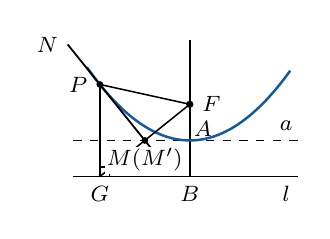
\begin{tikzpicture}[scale=1.02]
      % 抛物线 y = x^2 / 1.8, 焦点 F=(0, 0.45), 准线 l: y=-0.45, 直线 a: y=0
      \coordinate (F) at (0,0.45);
      \coordinate (A) at (0,0);
      \coordinate (B) at (0,-0.45);
      \coordinate (M) at (-0.56,0);
      \coordinate (G) at (-1.12,-0.45);
      \coordinate (P) at (-1.12,0.6969);
      \coordinate (N) at (-1.52,1.1947);

      % 准线 l 与直线 a, 轴 FB
      \draw[line width=0.65pt] (-1.45,-0.45) -- (1.35,-0.45);
      \node[below] at (1.20,-0.45) {\footnotesize $l$};
      \draw[dashed, line width=0.65pt] (-1.45,0) -- (1.35,0);
      \node[above] at (1.20,0) {\footnotesize $a$};
      \draw[line width=0.55pt] (0,1.25) -- (B);

      % 抛物线
      \draw[line width=0.9pt, curveblue, domain=-1.28:1.25, samples=60]
        plot (\x, {\x*\x/1.8});

      % 辅助线: F-M-G, G-P, P-F, 切线 N-P-M 延长 (斜率 -1.12/0.9 = -1.2444)
      \draw[line width=0.55pt] (F) -- (G);
      \draw[line width=0.55pt] (G) -- (P);
      \draw[line width=0.55pt] (P) -- (F);
      \draw[line width=0.65pt] (N) -- (-0.30,-0.3236);

      % 标记点与直角
      \draw[line width=0.45pt] (G) ++(0,0.12) -- ++(0.12,0) -- ++(0,-0.12);
      \fill (F) circle (1.3pt) node[right=1pt] {\footnotesize $F$};
      \fill (P) circle (1.2pt) node[left=1pt] {\footnotesize $P$};
      \fill (M) circle (1.2pt) node[below=2pt, fill=white, inner sep=0.8pt] {\footnotesize $M(M')$};
      \node[above right=-2pt] at (A) {\footnotesize $A$};
      \node[below] at (B) {\footnotesize $B$};
      \node[below] at (G) {\footnotesize $G$};
      \node[left] at (N) {\footnotesize $N$};
    \end{tikzpicture}
    \caption*{图\ 8.2}
  \end{minipage}
\end{figure}

这种画法，是根据抛物线切线的一个简单性质设计出来的。如图 8.2，设定点 $F$ 到定直线 $l$ 的距离为 $FB$，过 $FB$ 的中点 $A$ 作 $a \parallel l$。在 $a$ 上任取一点 $M$，作 $\angle FMN = 90^\circ$，现证 $MN$ 是抛物线的一条切线。

延长 $FM$ 交 $l$ 于 $G$，则 $FM = MG$。作 $GP \perp l$，交 $MN$ 于 $P$，由于 $\angle FMP = 90^\circ$，所以 $\triangle FMP \cong \triangle GMP$。从而得到 $PG = PF$，即 $P$ 点在以 $F$ 为焦点、$l$ 为准线的抛物线上，并且 $\angle GPM = \angle MPF$。过 $P$ 点作此抛物线的切线 $PM'$，根据切线的性质，$\angle FPM' = \angle GPM'$，可见 $PM$ 与 $PM'$ 重合，$MN$ 就是抛物线在 $P$ 点的切线。显然，$MN$ 是不会平行于 $BF$ 的。

\section{用三角板画椭圆}
\markboth{9. 用三角板画椭圆}{9. 用三角板画椭圆}

画一个辅助圆，设圆心是 $O$；在圆内另外再取一点 $F$。如图 9.1，让三角板的一条直角边通过 $F$ 点，直角顶点 $M$ 落在辅助圆周上的任意位置，然后沿着另一条直角边 $MN$ 画出一条直线。照这样画法画出若干条直线以后，再画一条与这些直线都相切的光滑曲线，就得到一个椭圆。

\begin{center}
  \begin{minipage}[t]{0.47\textwidth}
    \centering
    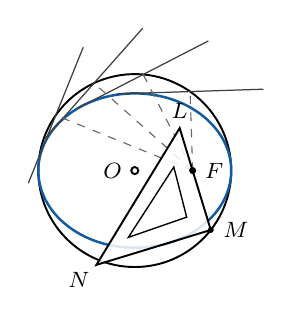
\begin{tikzpicture}[scale=0.98]
      % 辅助圆 a=1.25, O=(0,0), F=(0.75, 0), 椭圆 b=1.00
      \def\a{1.25}
      \def\b{1.00}
      \coordinate (O) at (0,0);
      \coordinate (F) at (0.75,0);

      \draw[line width=0.7pt] (O) circle (\a);
      \draw[line width=0.9pt, curveblue] (O) ellipse [x radius=\a, y radius=\b];

      % 上部几条切线(由圆周点 M0 产生)
      \foreach \ang in {55, 85, 115, 145} {
        \pgfmathsetmacro{\mx}{\a*cos(\ang)}
        \pgfmathsetmacro{\my}{\a*sin(\ang)}
        % 垂直于 FM=(mx-0.75, my) 的方向 (-my, mx-0.75)
        \pgfmathsetmacro{\tx}{-\my}
        \pgfmathsetmacro{\ty}{\mx - 0.75}
        \pgfmathsetmacro{\len}{sqrt(\tx*\tx + \ty*\ty)}
        \pgfmathsetmacro{\ux}{\tx/\len}
        \pgfmathsetmacro{\uy}{\ty/\len}
        \draw[line width=0.45pt, black!75] ({\mx - 0.95*\ux}, {\my - 0.95*\uy}) -- ({\mx + 0.95*\ux}, {\my + 0.95*\uy});
        \draw[line width=0.4pt, dashed, black!60] (F) -- (\mx, \my);
      }

      % 三角板: M 在圆周 -38 度处
      \coordinate (M) at ({\a*cos(-38)},{\a*sin(-38)});
      % FM 方向: M - F = (0.985 - 0.75, -0.7696) = (0.235, -0.7696)
      % 从 M 向上指向 F 方向: (-0.2921, 0.9564)
      % 向左下垂直方向: (-0.9564, -0.2921)
      \coordinate (L) at ($(M) + 1.38*(-0.2921, 0.9564)$);
      \coordinate (N) at ($(M) + 1.55*(-0.9564, -0.2921)$);
      \draw[line width=0.7pt, fill=white, fill opacity=0.85] (M) -- (L) -- (N) -- cycle;
      % 内部镂空三角形
      \coordinate (M1) at ($(M) + 0.25*(-0.2921, 0.9564) + 0.25*(-0.9564, -0.2921)$);
      \coordinate (L1) at ($(M) + 0.92*(-0.2921, 0.9564) + 0.22*(-0.9564, -0.2921)$);
      \coordinate (N1) at ($(M) + 0.22*(-0.2921, 0.9564) + 1.05*(-0.9564, -0.2921)$);
      \draw[line width=0.5pt] (M1) -- (L1) -- (N1) -- cycle;

      \draw[fill=white, line width=0.7pt] (O) circle (1.3pt) node[left=1pt] {\footnotesize $O$};
      \fill (F) circle (1.3pt) node[right=1pt] {\footnotesize $F$};
      \fill (M) circle (1.1pt) node[right=1pt] {\footnotesize $M$};
      \node[above] at (L) {\footnotesize $L$};
      \node[below left=-1pt] at (N) {\footnotesize $N$};
    \end{tikzpicture}
    \par\vspace{3pt}{\footnotesize 图\ 9.1}
  \end{minipage}
  \hfill
  \begin{minipage}[t]{0.47\textwidth}
    \centering
    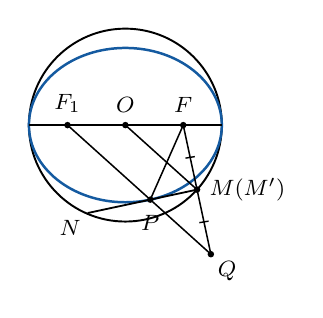
\begin{tikzpicture}[scale=0.98]
      % 辅助圆 a=1.25, O=(0,0), F=(0.75, 0), F1=(-0.75, 0), 椭圆 b=1.00
      \def\a{1.25}
      \def\b{1.00}
      \coordinate (O) at (0,0);
      \coordinate (F) at (0.75,0);
      \coordinate (F1) at (-0.75,0);

      \draw[line width=0.7pt] (O) circle (\a);
      \draw[line width=0.9pt, curveblue] (O) ellipse [x radius=\a, y radius=\b];

      % M 在 -42 度: M = (0.9289, -0.8364)
      \coordinate (M) at ({\a*cos(-42)},{\a*sin(-42)});
      % Q = 2M - F = (1.1079, -1.6728)
      \coordinate (Q) at ($(M) + (M) - (F)$);
      % 切线 MN 方向垂直于 FM = (0.1789, -0.8364) -> (-0.8364, -0.1789), 单位化 (-0.9779, -0.2091)
      \coordinate (N) at ($(M) + 1.45*(-0.9779, -0.2091)$);
      % P 是 F1Q 与 MN 的交点
      \path[name path=f1q] (F1) -- (Q);
      \path[name path=mn] (M) -- (N);
      \path[name intersections={of=f1q and mn, by=P}];

      \draw[line width=0.6pt] (-1.25,0) -- (1.25,0);
      \draw[line width=0.55pt] (F) -- (Q);
      \draw[line width=0.55pt] (F1) -- (Q);
      \draw[line width=0.55pt] (O) -- (M);
      \draw[line width=0.55pt] (F) -- (P);
      \draw[line width=0.65pt] (M) -- (N);

      % 等长刻度标志 (FM = MQ)
      \coordinate (K1) at ($(F)!0.5!(M)$);
      \coordinate (K2) at ($(M)!0.5!(Q)$);
      \draw[line width=0.5pt] ($(K1) + (-0.06,-0.01)$) -- ($(K1) + (0.06,0.01)$);
      \draw[line width=0.5pt] ($(K2) + (-0.06,-0.01)$) -- ($(K2) + (0.06,0.01)$);

      % 标记点
      \fill (F1) circle (1.2pt) node[above=1pt] {\footnotesize $F_1$};
      \fill (O) circle (1.2pt) node[above=1pt] {\footnotesize $O$};
      \fill (F) circle (1.2pt) node[above=1pt] {\footnotesize $F$};
      \fill (M) circle (1.2pt) node[right=1pt] {\footnotesize $M(M')$};
      \fill (P) circle (1.2pt) node[below=2pt] {\footnotesize $P$};
      \fill (Q) circle (1.2pt) node[below right=-1pt] {\footnotesize $Q$};
      \node[below left=-1pt] at (N) {\footnotesize $N$};
    \end{tikzpicture}
    \par\vspace{3pt}{\footnotesize 图\ 9.2}
  \end{minipage}
\end{center}

椭圆的这种画法是根据椭圆的切线的性质设计出来的。如图 9.2，设 $\odot O$ 的半径为 $a$，$F$ 是圆内一点，$F_1$ 与 $O$、$F$ 在一直线上，且 $F_1O = OF$。$M$ 为 $\odot O$ 上任意一点，作 $\angle FMN = 90^\circ$，现证 $MN$ 是椭圆的一条切线。

延长 $FM$ 至 $Q$，使 $MQ = FM$，连结 $F_1Q$，交 $MN$ 于 $P$ 点，连 $FP$。因为 $\angle FMP = 90^\circ$，所以 $\triangle FMP \cong \triangle QMP$，$PF = PQ$，$\angle FPM = \angle QPM$。又因为 $O$ 点是 $F_1F$ 的中点，所以 $F_1Q \parallel OM$，且 $F_1Q = 2OM = 2a$，即 $PF_1 + PF = PF_1 + PQ = 2a$，所以 $P$ 点在以 $F$、$F_1$ 为焦点的，长轴为 $2a$ 的椭圆上。过 $P$ 点作此椭圆的切线 $PM'$，由切线的性质知，$\angle FPM' = \angle QPM'$，可见 $PM$ 与 $PM'$ 重合，$MN$ 就是椭圆在 $P$ 点的切线。

若图 9.1 中的 $F$ 点在圆外，那末用同样的作法得到的就是双曲线的一支。读者有兴趣可以仿照上面写出证明，试试自己举一反三的本领。

\section{垂足曲线和反垂足曲线}
\markboth{10. 垂足曲线和反垂足曲线}{10. 垂足曲线和反垂足曲线}

利用三角板画曲线的方法，不但可以用来画抛物线、椭圆和双曲线，而且可以用来画许多其它曲线。这种画法是有垂足曲线和反垂足曲线作为背景的。

\noindent
\begin{minipage}[t]{0.53\textwidth}
  \setlength{\parindent}{2em}
  在图 10.1 中有一条曲线 $c$，设 $M$ 是平面曲线 $c$ 上的任意点，$O$ 是这张平面内的一个定点。过 $M$ 作曲线 $c$ 的切线 $MT$；再作 $OP \perp MT$，垂足为 $P$。当 $M$ 沿曲线 $c$ 移动时，垂足 $P$ 也画出一条曲线 $s$，$s$ 就叫做曲线 $c$ 关于 $O$ 点的垂足曲线。反过来，$c$ 叫做曲线 $s$ 关于 $O$ 点的反垂足曲线。
\end{minipage}
\hfill
\begin{minipage}[t]{0.44\textwidth}
  \centering
  \vspace{-2pt}
  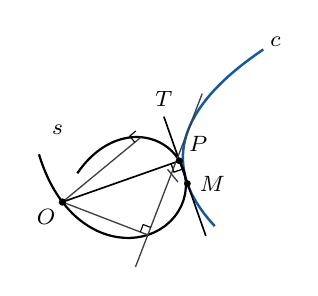
\begin{tikzpicture}[scale=1.02]
    \coordinate (O) at (-0.75, -0.55);

    % 曲线 c
    \draw[line width=0.9pt, curveblue, domain=-0.85:1.35, samples=60]
      plot ({0.75 + 0.55*\x*\x}, \x);
    \node[above right=-1pt] at ({0.75 + 0.55*1.35*1.35}, 1.30) {\footnotesize $c$};

    % 垂足曲线 s
    \draw[line width=0.8pt, black, domain=-1.75:1.85, samples=80]
      plot ({
        0.75 + 0.55*\x*\x + ( ((-0.75 - 0.75 - 0.55*\x*\x)*1.1*\x + (-0.55 - \x)) / (1.21*\x*\x + 1) ) * 1.1*\x
      }, {
        \x + ( ((-0.75 - 0.75 - 0.55*\x*\x)*1.1*\x + (-0.55 - \x)) / (1.21*\x*\x + 1) )
      });

    % 主点 t = -0.32
    \pgfmathsetmacro{\ta}{-0.32}
    \pgfmathsetmacro{\mx}{0.75 + 0.55*\ta*\ta}
    \pgfmathsetmacro{\my}{\ta}
    \pgfmathsetmacro{\tx}{1.1*\ta}
    \pgfmathsetmacro{\ty}{1.0}
    \pgfmathsetmacro{\lam}{((-0.75-\mx)*\tx + (-0.55-\my)*\ty)/(\tx*\tx + \ty*\ty)}
    \pgfmathsetmacro{\px}{\mx + \lam*\tx}
    \pgfmathsetmacro{\py}{\my + \lam*\ty}
    \coordinate (M) at (\mx, \my);
    \coordinate (P) at (\px, \py);
    \coordinate (T) at ({\px + 0.55*\tx}, {\py + 0.55*\ty});
    \draw[line width=0.6pt] ({\px + 0.55*\tx}, {\py + 0.55*\ty}) -- ({\mx - 0.65*\tx}, {\my - 0.65*\ty});
    \draw[line width=0.6pt] (O) -- (P);
    \pgfmathsetmacro{\ux}{\tx/sqrt(\tx*\tx+\ty*\ty)}
    \pgfmathsetmacro{\uy}{\ty/sqrt(\tx*\tx+\ty*\ty)}
    \pgfmathsetmacro{\nx}{(\px+0.75)/sqrt((\px+0.75)^2+(\py+0.55)^2)}
    \pgfmathsetmacro{\ny}{(\py+0.55)/sqrt((\px+0.75)^2+(\py+0.55)^2)}
    \draw[line width=0.45pt] (P) ++(-0.11*\ux, -0.11*\uy) -- ++(-0.11*\nx, -0.11*\ny) -- ++(0.11*\ux, 0.11*\uy);

    % 另外两条切线与垂线: t = 0.35 和 t = -0.75
    \foreach \tb in {0.35, -0.75} {
      \pgfmathsetmacro{\mxb}{0.75 + 0.55*\tb*\tb}
      \pgfmathsetmacro{\myb}{\tb}
      \pgfmathsetmacro{\txb}{1.1*\tb}
      \pgfmathsetmacro{\tyb}{1.0}
      \pgfmathsetmacro{\lamb}{((-0.75-\mxb)*\txb + (-0.55-\myb)*\tyb)/(\txb*\txb + \tyb*\tyb)}
      \pgfmathsetmacro{\pxb}{\mxb + \lamb*\txb}
      \pgfmathsetmacro{\pyb}{\myb + \lamb*\tyb}
      \draw[line width=0.48pt, black!75] ({\pxb - 0.40*\txb}, {\pyb - 0.40*\tyb}) -- ({\mxb + 0.45*\txb}, {\myb + 0.45*\tyb});
      \draw[line width=0.48pt, black!75] (O) -- (\pxb, \pyb);
      \pgfmathsetmacro{\uxb}{\txb/sqrt(\txb*\txb+\tyb*\tyb)}
      \pgfmathsetmacro{\uyb}{\tyb/sqrt(\txb*\txb+\tyb*\tyb)}
      \pgfmathsetmacro{\nxb}{(\pxb+0.75)/sqrt((\pxb+0.75)^2+(\pyb+0.55)^2)}
      \pgfmathsetmacro{\nyb}{(\pyb+0.55)/sqrt((\pxb+0.75)^2+(\pyb+0.55)^2)}
      \draw[line width=0.4pt] (\pxb, \pyb) ++(0.10*\uxb, 0.10*\uyb) -- ++(-0.10*\nxb, -0.10*\nyb) -- ++(-0.10*\uxb, -0.10*\uyb);
    }

    \fill (O) circle (1.3pt) node[below left=-1pt] {\footnotesize $O$};
    \fill (M) circle (1.2pt) node[right=1pt] {\footnotesize $M$};
    \fill (P) circle (1.2pt) node[above right=0pt] {\footnotesize $P$};
    \node[above] at (T) {\footnotesize $T$};
    \node[left] at (-0.62, 0.35) {\footnotesize $s$};
  \end{tikzpicture}
  \par\vspace{4pt}{\footnotesize 图\ 10.1}
\end{minipage}

图 10.1 中的 $\angle OPM$ 可以用三角板来实现，这就是三角板画法的本质。具体地说，让三角板的一条直角边通过 $O$ 点，另一条直角边与曲线 $c$ 相切，这时直角顶点 $P$ 的位置就指出了 $c$ 关于 $O$ 点的垂足曲线 $s$。

如果让三角板的一条直角边通过 $O$ 点，直角顶点 $P$ 在曲线 $s$ 上移动，这时另一条直角边就给出了一族直线，与这些直线都相切的光滑曲线，就是 $s$ 关于 $O$ 点的反垂足曲线 $c$。

根据前面几节的讨论，可以知道，抛物线关于焦点的垂足曲线是直线，椭圆和双曲线关于焦点的垂足曲线都是圆。反过来，直线关于线外一点的反垂足曲线是抛物线，圆周关于圆内一点的反垂足曲线是椭圆，圆周关于圆外一点的反垂足曲线是双曲线。正是利用这些性质，设计出了利用三角板画抛物线、椭圆和双曲线的方法。


% --- 批次 2：第 11–20 节 ---
\section{摆线}
\markboth{11. 摆线}{11. 摆线}

当动圆 $C$ 沿着定直线 $l$ 滚动（没有滑动）时，动圆圆周上一点 $M$ 所画出的曲线叫做摆线，又叫旋轮线（图 11.1）。摆线在它与定直线 $l$ 的两个相邻交点之间的部分叫做一个拱；摆线最高点到定直线的距离 $2r$ 叫做拱高。

\begin{center}
  \begin{minipage}{\linewidth}
    \centering
    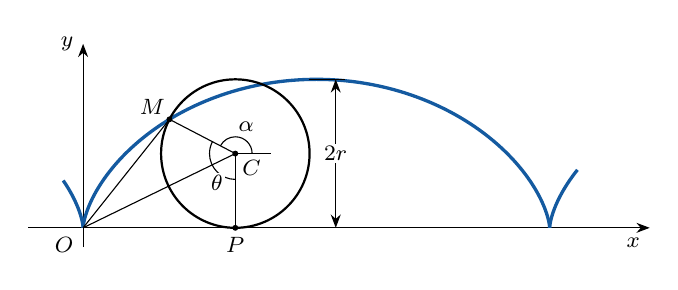
\begin{tikzpicture}[scale=0.82, >=Stealth, font=\footnotesize]
      % 参数 r = 1.15
      \def\r{1.15}
      \def\th{2.05}
      \pgfmathsetmacro{\cx}{\r*\th}
      \pgfmathsetmacro{\cy}{\r}
      \pgfmathsetmacro{\mx}{\r*(\th - sin(\th r))}
      \pgfmathsetmacro{\my}{\r*(1 - cos(\th r))}
      \pgfmathsetmacro{\angM}{deg(1.5*pi - \th)}

      % 坐标轴
      \draw[->] (-0.85, 0) -- ({2*pi*\r + 1.55}, 0) node[below left] {$x$};
      \draw[->] (0, -0.3) -- (0, {2*\r + 0.55}) node[left] {$y$};
      \node[below left] at (0, 0) {$O$};

      % 摆线（前一拱末端 + 完整一拱 + 后一拱起始）
      \draw[very thick, curveblue, smooth, domain=-1.2:0, samples=30]
        plot ({\r*(\x - sin(\x r))}, {\r*(1 - cos(\x r))});
      \draw[very thick, curveblue, smooth, domain=0:{2*pi}, samples=90]
        plot ({\r*(\x - sin(\x r))}, {\r*(1 - cos(\x r))});
      \draw[very thick, curveblue, smooth, domain={2*pi}:{2*pi+1.35}, samples=35]
        plot ({\r*(\x - sin(\x r))}, {\r*(1 - cos(\x r))});

      % 动圆 C
      \coordinate (O) at (0, 0);
      \coordinate (C) at (\cx, \cy);
      \coordinate (P) at (\cx, 0);
      \coordinate (M) at (\mx, \my);
      \coordinate (R) at ({\cx + 0.55}, \cy);

      \draw[thick] (C) circle (\r);
      \draw[thin] (O) -- (C);
      \draw[thin] (O) -- (M);
      \draw[thin] (C) -- (M);
      \draw[thin] (C) -- (P);
      \draw[thin] (C) -- (R);

      % 角度标注 theta（从 CP 顺时针到 CM）和 alpha（从向右射线逆时针到 CM）
      \draw (C) ++(270:0.40) arc (270:\angM:0.40);
      \node[fill=white, inner sep=0.8pt] at ($(C)+(238:0.54)$) {$\theta$};
      \draw (C) ++(0:0.26) arc (0:\angM:0.26);
      \node at ($(C)+(68:0.45)$) {$\alpha$};

      % 拱高 2r 标注
      \draw[thin] ({\r*pi - 0.12}, {2*\r}) -- ({\r*pi + 0.45}, {2*\r});
      \draw[<->, thin] ({\r*pi + 0.30}, 0) -- ({\r*pi + 0.30}, {2*\r})
        node[midway, fill=white, inner sep=1pt] {$2r$};

      % 点与标注
      \fill (C) circle (1.3pt) node[below right, xshift=-1pt, yshift=1pt] {$C$};
      \fill (M) circle (1.3pt) node[above left, inner sep=1.5pt] {$M$};
      \fill (P) circle (1.3pt) node[below] {$P$};
    \end{tikzpicture}
    \captionof*{figure}{图 11.1}
  \end{minipage}
\end{center}

一个骑自行车的人，滚动的车轮偶然从地面上粘起一张糖纸，当车轮继续向前时，这张糖纸就在空中画出一条摆线。车轮每旋转一周，糖纸就画出摆线的一拱。

现在推导摆线的方程。为了写得紧凑些，这里和以下许多地方将用一点简单的向量写法：用 $(a, b)$ 表示在 $x$ 轴和 $y$ 轴上的分量依次为 $a$、$b$ 的向量；两个向量相加，其对应分量相加。如图 11.1，取定直线 $l$ 为 $x$ 轴，并使动圆位于 $x$ 轴上方。又设动圆的圆心在 $y$ 轴上时，$M$ 恰好在坐标原点。记圆半径为 $r$，则当它滚动到图中位置时，由于 $\overrightarrow{OM} = \overrightarrow{OC} + \overrightarrow{CM}$，$\alpha = \frac{3}{2}\pi - \theta$，所以 $M$ 点的坐标可由向量 $\overrightarrow{OM}$ 的坐标表示式给出：
\begin{align*}
  (x, y) &= (OP, PC) + (CM\cos\alpha, CM\sin\alpha) \\
         &= (r\theta, r) + (-r\sin\theta, -r\cos\theta) \\
         &= (r\theta - r\sin\theta, r - r\cos\theta).
\end{align*}
即 $M$ 点的坐标为
\begin{gather*}
  x = r(\theta - \sin\theta), \\
  y = r(1 - \cos\theta).
\end{gather*}
这就是摆线的参数方程。当 $\theta$ 从 $0$ 变化到 $2\pi$ 时，动点 $M(x, y)$ 描绘出摆线的一拱。

\section{利用微分三角形求曲线的弧长}
\markboth{12. 利用微分三角形求曲线的弧长}{12. 利用微分三角形求曲线的弧长}

在讨论曲线的性质和应用时，很多问题都与曲线的弧长有关，这时可以利用下面介绍的微分三角形。

如图 12.1，设 $M(x, y)$ 是曲线 $\Gamma$ 上的任意点，$N(x + dx, y + \Delta y)$ 是曲线 $\Gamma$ 上靠近 $M$ 的点。为了看得清楚，图中把 $N$ 与 $M$ 之间的距离有意画大了。又设图中 $NP$ 平行于 $y$ 轴，$MP$ 平行于 $x$ 轴，$MQ$ 是曲线 $\Gamma$ 在 $M$ 点的切线，$MQ$ 与 $x$ 轴的夹角为 $\alpha$，那么从 $MP = dx$ 和
\[
  \tg\alpha = \frac{dy}{dx}
\]
可得
\[
  PQ = dy,\quad PN = \Delta y = dy + QN.
\]

\begin{center}
  \begin{minipage}{\linewidth}
    \centering
    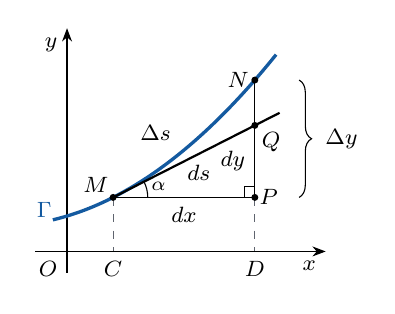
\begin{tikzpicture}[scale=0.90, >=Stealth, font=\footnotesize]
      % 坐标轴
      \draw[->] (-0.45, 0) -- (3.65, 0) node[below left] {$x$};
      \draw[->] (0, -0.3) -- (0, 3.15) node[below left] {$y$};
      \node[below left] at (0, 0) {$O$};

      % 曲线 Gamma: y = 0.5 + 0.30*x + 0.16*x^2
      \draw[very thick, curveblue, smooth, domain=-0.2:2.95, samples=80]
        plot (\x, {0.5 + 0.30*\x + 0.16*\x*\x});
      \node[curveblue, left] at (-0.08, 0.58) {$\Gamma$};

      % 关键点坐标
      \coordinate (M) at (0.65, 0.7626);
      \coordinate (N) at (2.65, 2.4186);
      \coordinate (P) at (2.65, 0.7626);
      \coordinate (Q) at (2.65, 1.7786);
      \coordinate (C) at (0.65, 0);
      \coordinate (D) at (2.65, 0);
      \coordinate (T) at (3.00, {0.7626 + 0.508*(3.00 - 0.65)});

      % 辅助垂线与水平线
      \draw[dashed, mutedgray] (M) -- (C) node[below, black] {$C$};
      \draw[dashed, mutedgray] (P) -- (D) node[below, black] {$D$};
      \draw[thin] (M) -- (P);
      \draw[thin] (P) -- (N);

      % 切线 MQ（略微延长）
      \draw[thick] (M) -- (T);

      % 直角标记
      \draw ($(P)+(-0.15,0)$) -- ($(P)+(-0.15,0.15)$) -- ($(P)+(0,0.15)$);

      % 夹角 alpha
      \pic[draw, angle radius=0.44cm, angle eccentricity=1.35, "\scriptsize$\alpha$"] {angle=P--M--Q};

      % 点标记
      \fill (M) circle (1.4pt) node[above left, inner sep=1.5pt] {$M$};
      \fill (N) circle (1.4pt) node[left, inner sep=2pt] {$N$};
      \fill (P) circle (1.4pt) node[right, inner sep=1.5pt] {$P$};
      \fill (Q) circle (1.4pt) node[below right, xshift=-1pt, yshift=1pt] {$Q$};

      % 边长与增量标注
      \node[below] at ($(M)!0.5!(P)$) {$dx$};
      \node[left] at ($(P)!0.5!(Q)$) {$dy$};
      \node[below right, inner sep=1pt] at ($(M)!0.5!(Q)$) {$ds$};
      \node[above left, inner sep=2pt] at (1.55, 1.48) {$\Delta s$};

      % 右侧大括号标注 Delta y
      \draw[decorate, decoration={brace, amplitude=4.5pt, raise=16pt}]
        (N) -- (P) node[midway, right=22pt] {$\Delta y$};
    \end{tikzpicture}
    \captionof*{figure}{图 12.1}
  \end{minipage}
\end{center}

当 $dx$ 非常小时，$QN$ 比 $dy$ 小得多，可以忽略，这时可以近似地认为 $N$ 点与 $Q$ 点重合。相应地，一小段曲线弧 $\arc{MN}$ 可以近似看成切线上的对应线段 $MQ$。用 $\Delta s$ 表示弧 $\arc{MN}$ 的长度，$ds$ 表示线段 $MQ$ 的长度，那么当 $dx$ 非常小时就有
\[
  \Delta y \approx dy,\quad \Delta s \approx ds.
\]
因而，正像 $dy$ 叫做 $y$ 的微分一样，$ds$ 叫做弧长 $s$ 的微分。对于直角三角形 $MPQ$，应用勾股定理得到
\[
  (ds)^2 = (dx)^2 + (dy)^2.
\]
通常把上式简写成
\[
  ds^2 = dx^2 + dy^2,
\]

\noindent
\begin{minipage}[c]{0.38\textwidth}
  \centering
  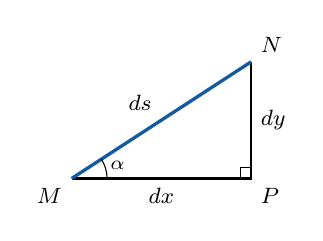
\begin{tikzpicture}[scale=0.76, font=\footnotesize]
    \coordinate (M) at (0, 0);
    \coordinate (P) at (3.0, 0);
    \coordinate (N) at (3.0, 1.95);

    \draw[thick] (M) -- (P) -- (N);
    \draw[very thick, curveblue] (M) -- (N);

    % 直角标记
    \draw ($(P)+(-0.18,0)$) -- ($(P)+(-0.18,0.18)$) -- ($(P)+(0,0.18)$);
    % 夹角 alpha
    \pic[draw, angle radius=0.45cm, angle eccentricity=1.35, "\scriptsize$\alpha$"] {angle=P--M--N};

    % 顶点与边标注
    \node[below left] at (M) {$M$};
    \node[below right] at (P) {$P$};
    \node[above right] at (N) {$N$};
    \node[below] at ($(M)!0.5!(P)$) {$dx$};
    \node[right] at ($(P)!0.5!(N)$) {$dy$};
    \node[above left] at ($(M)!0.5!(N)$) {$ds$};
  \end{tikzpicture}
  \captionof*{figure}{图 12.2}
\end{minipage}\hfill
\begin{minipage}[c]{0.58\textwidth}
  \noindent 并且把线段 $MQ$ 画成与曲线弧 $\arc{MN}$ 重合在一起，使图 12.1 简化成图 12.2 的形状。图 12.2 中由微分 $dx$、$dy$ 和 $ds$ 组成的直角三角形就叫做微分三角形。微分三角形很容易记住，并且从它立刻可写出
  \[
    ds = \sqrt{dx^2 + dy^2}.
  \]
\end{minipage}

$ds$ 只不过是一小段弧长。再将 $ds$ 积分，就能求出弧长 $s$ 了。具体说来，如果曲线是由参数方程 $x = \varphi(\theta)$，$y = f(\theta)$ 给出的，用撇号表示对参数 $\theta$ 的导数，那么
\[
  ds = \sqrt{(x'\dd\theta)^2 + (y'\dd\theta)^2} = \sqrt{x'^2 + y'^2}\dd\theta,
\]
因而曲线在 $\theta = \theta_1$ 和 $\theta = \theta_2$ 的两点间的弧长是
\[
  s = \int_{\theta_1}^{\theta_2} \sqrt{x'^2 + y'^2}\dd\theta.
\]

直角坐标方程 $y = f(x)$ 可看成参数方程的特例，这时参数 $\theta = x$，因而 $x' = 1$，曲线在 $x = x_1$ 和 $x = x_2$ 的两点间的弧长是
\[
  s = \int_{x_1}^{x_2} \sqrt{1 + y'^2}\dd x.
\]

作为例子，我们现在来求摆线一拱的长。摆线方程是
\[
  x = r(\theta - \sin\theta),\quad y = r(1 - \cos\theta).\quad (0 \leqslant \theta \leqslant 2\pi)
\]
由此得到摆线一拱的弧长是
\begin{align*}
  s &= \int_{0}^{2\pi} \sqrt{x'^2 + y'^2}\dd\theta \\
    &= \int_{0}^{2\pi} \sqrt{r^2(1 - \cos\theta)^2 + r^2\sin^2\theta}\dd\theta \\
    &= \int_{0}^{2\pi} r\sqrt{1 - 2\cos\theta + \cos^2\theta + \sin^2\theta}\dd\theta \\
    &= \int_{0}^{2\pi} r\sqrt{2(1 - \cos\theta)}\dd\theta
     = \int_{0}^{2\pi} r\sqrt{4\sin^2\frac{\theta}{2}}\dd\theta \\
    &= 2r\int_{0}^{2\pi} \sin\frac{\theta}{2}\dd\theta
     = \left.-4r\cos\frac{\theta}{2}\right|_{0}^{2\pi} = 8r.
\end{align*}
由于摆线的拱高是 $2r$，所以摆线一拱的弧长恰好是拱高的 $4$ 倍。

\section{摆线滑梯}
\markboth{13. 摆线滑梯}{13. 摆线滑梯}

\noindent
\begin{minipage}[c]{0.53\textwidth}
  \hspace*{2em}如图 13.1，把半拱摆线 $\arc{OMA}$ 连同 $y$ 轴一起翻转到 $x$ 轴下方来，并且连结 $OA$，就做成了两个滑梯：一个是普通滑梯，它的滑道是斜线 $OA$；另一个是摆线滑梯，它的滑道是摆线弧 $\arc{OMA}$。现在向你提出一个问题：如果 $O$ 点有甲、乙两个小孩，甲沿普通滑梯滑下，乙同时沿摆线滑梯滑下，谁先滑到底？
\end{minipage}\hfill
\begin{minipage}[c]{0.44\textwidth}
  \centering
  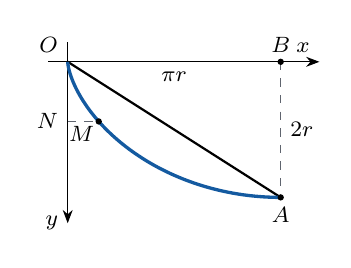
\begin{tikzpicture}[scale=0.82, >=Stealth, font=\footnotesize]
    % 摆线尺度 r_scale = 1.05, theta in [0, pi]
    \def\rs{1.05}
    \coordinate (O) at (0, 0);
    \coordinate (B) at ({\rs*pi}, 0);
    \coordinate (A) at ({\rs*pi}, {-2*\rs});
    % 点 M 取 theta = 1.45 rad
    \coordinate (M) at ({\rs*(1.45 - sin(1.45 r))}, {-\rs*(1 - cos(1.45 r))});
    \coordinate (N) at (0, {-\rs*(1 - cos(1.45 r))});

    % 坐标轴（x 向右，y 向下）
    \draw[->] (-0.3, 0) -- ({\rs*pi + 0.6}, 0) node[above left] {$x$};
    \draw[->] (0, 0.3) -- (0, {-2*\rs - 0.4}) node[left] {$y$};
    \node[above left] at (O) {$O$};

    % 辅助虚线
    \draw[dashed, mutedgray] (B) -- (A) node[midway, right, black] {$2r$};
    \draw[dashed, mutedgray] (N) -- (M);

    % 普通滑梯 OA（斜线）
    \draw[thick] (O) -- (A);

    % 摆线滑梯 OMA（参数方程精确绘制）
    \draw[very thick, curveblue, smooth, domain=0:pi, samples=80]
      plot ({\rs*(\x - sin(\x r))}, {-\rs*(1 - cos(\x r))});

    % 点与标签
    \fill (A) circle (1.4pt) node[below] {$A$};
    \fill (B) circle (1.4pt) node[above] {$B$};
    \fill (M) circle (1.4pt) node[below left, inner sep=1.5pt] {$M$};
    \node[left] at (N) {$N$};
    \node[below] at ($(O)!0.5!(B)$) {$\pi r$};
  \end{tikzpicture}
  \captionof*{figure}{图 13.1}
\end{minipage}

你大概会回答是甲吧，错了！你的回答一定是因为甲走过的路程较短。但是请你细想一下，现在问题是问谁花的时间最少，这就不但与路程长短有关，而且跟滑行的速度有关了。甲沿着斜线 $OA$ 下滑，是做匀加速运动，速度从 $0$ 开始，缓慢而均匀地增大。乙沿摆线下滑，速度也是从 $0$ 开始，但是刚开始滑行就是一段陡坡，速度迅速增大，使得乙的滑行速度比甲快。虽然比甲多走一点路，但究竟谁先到达终点，就很难说了！如果乙的路线选择得非常巧妙，速度增大得又快，路程的长度增加得又少，为什么不可以先滑到底呢？

还是来算一下，看看究竟谁先滑到底。

假定滑梯是绝对光滑的，小孩从 $O$ 点开始下滑时，初速度是 $0$。设他下滑到点 $M$ 时，离地面的高度下降了 $y$，那么根据力学原理知道，他的重力势能就减少了 $mgy$，这里 $m$ 是小孩的质量，$g$ 是重力加速度。又设这时他的速度大小是 $v$，因而这时的动能是 $\frac{1}{2}mv^2$。由于开始下滑时动能是零，根据能量守恒定律，现在的这些动能是由减少的势能转化而来的，由此得到
\begin{gather*}
  \frac{1}{2}mv^2 = mgy, \\
  \therefore\ v = \sqrt{2gy}.
\end{gather*}
另一方面，速度 $v$ 等于路程 $s$ 对时间 $t$ 的导数 $\frac{ds}{dt}$，代入上式得
\begin{gather*}
  \frac{ds}{dt} = \sqrt{2gy}, \\
  \therefore\ dt = \frac{ds}{\sqrt{2gy}}.
\end{gather*}
设滑行曲线的参数方程是 $x = \varphi(\theta)$，$y = f(\theta)$，用撇号表示对参数 $\theta$ 的导数，利用微分三角形（第 12 节）得到
\begin{gather*}
  ds = \sqrt{x'^2 + y'^2}\dd\theta, \\
  \therefore\ dt = \frac{\sqrt{x'^2 + y'^2}}{\sqrt{2gy}}\dd\theta.
\end{gather*}
积分，就得到从 $\theta = \theta_1$ 的点下滑到 $\theta = \theta_2$ 的点所需的时间是
\[
  T = \int_{\theta_1}^{\theta_2} \frac{\sqrt{x'^2 + y'^2}}{\sqrt{2gy}}\dd\theta.
\]
如用直角坐标方程，则
\[
  T = \int_{x_1}^{x_2} \frac{\sqrt{1 + y'^2}}{\sqrt{2gy}}\dd x.
\]

读者注意，以上推导公式的过程，与滑行路线的形状无关，因而这个公式对于普通滑梯和摆线滑梯以至任何滑梯都同样适用。先考虑普通滑梯，它的滑道是连接点 $O(0, 0)$ 和 $A(\pi r, 2r)$ 的线段，其方程为
\[
  y = \frac{2}{\pi}x.\quad (0 \leqslant x \leqslant \pi r)
\]
这时滑完全程所需的时间是
\begin{align*}
  T_1 &= \int_{x_1}^{x_2} \frac{\sqrt{1 + y'^2}}{\sqrt{2gy}}\dd x
       = \int_{0}^{\pi r} \frac{\sqrt{1 + \left(\frac{2}{\pi}\right)^2}}{\sqrt{\frac{4g}{\pi}x}}\dd x \\
      &= \sqrt{\frac{\pi}{g}\left(1 + \frac{4}{\pi^2}\right)} \int_{0}^{\pi r} \frac{dx}{2\sqrt{x}} \\
      &= \left.\sqrt{\frac{\pi}{g}\left(1 + \frac{4}{\pi^2}\right)} \cdot \sqrt{x}\right|_{0}^{\pi r} \\
      &= \sqrt{\frac{r}{g}(\pi^2 + 4)}.
\end{align*}

其次考虑摆线滑梯。它的滑道是半拱摆线弧，其参数方程可以写成
\[
  x = r(\theta - \sin\theta),\quad y = r(1 - \cos\theta).\quad (0 \leqslant \theta \leqslant \pi)
\]
因而沿着摆线滑梯滑到底所需的时间是
\begin{align*}
  T_2 &= \int_{0}^{\pi} \frac{\sqrt{x'^2 + y'^2}}{\sqrt{2gy}}\dd\theta
       = \int_{0}^{\pi} \frac{\sqrt{2r^2(1 - \cos\theta)}}{\sqrt{2gr(1 - \cos\theta)}}\dd\theta \\
      &= \sqrt{\frac{r}{g}} \int_{0}^{\pi} d\theta
       = \left.\sqrt{\frac{r}{g}}\,\theta\right|_{0}^{\pi}
       = \sqrt{\frac{r}{g}}\,\pi.
\end{align*}
由于
\[
  \sqrt{\frac{r}{g}(\pi^2 + 4)} > \sqrt{\frac{r}{g}\,\pi^2} = \sqrt{\frac{r}{g}}\,\pi,
\]
所以 $T_1 > T_2$，即普通滑梯上的小孩后到终点，摆线滑梯上的小孩先到终点。

\section{最速降线}
\markboth{14. 最速降线}{14. 最速降线}

欧洲的数学界在十七世纪时盛行一种挑战的风气：一个人公开提出一个或一些数学难题，大家都来做，看谁做得快、做得对、做得好。1696年，瑞士数学家约翰·贝努利提出一个难题向全欧洲的数学家挑战，题目的大意是：设在竖直平面内有一条曲线，一个质点由于重力的作用，从这条曲线的较高的端点沿曲线滑到较低的端点，问这条曲线是什么形状时，滑行所需的时间最短？（摩擦和空气阻力都忽略）这就是著名的“最速降线”问题。

设两个端点在竖直平面内的直角坐标是 $(0, 0)$ 和 $(a, b)$，曲线方程是 $y = f(x)$。曲线要通过这两点，所以 $f(0) = 0$，$f(a) = b$。根据第 13 节中导出的公式，沿曲线 $y = f(x)$ 滑行所需的时间是
\[
  T = \int_{0}^{a} \frac{\sqrt{1 + y'^2}}{\sqrt{2gy}}\dd x.
\]
问题归结为求函数 $y = f(x)$，满足条件 $f(0) = 0$，$f(a) = b$，并且使由上面的定积分得到的数 $T$ 取最小值。

这个问题看上去好象是个很普通的极值问题，但只要仔细一分析，就知道它非同寻常。人们熟知的极值问题，是函数已经确定，再求函数的极大值或极小值。而现在是不知道函数的表达式，倒过来要求出一种函数，使得整个式子达到极小。很显然，这是一种崭新的问题。因而用当时所知道的各种数学工具，包括微分法在内，都难以对付这种陌生而复杂的极值问题。

经过一番努力，这个问题还是有几个人解出来了；解答者除去挑战人约翰·贝努利自己之外，还有牛顿、莱布尼兹、约翰的哥哥雅各·贝努利等。答案就是上一节中那倒放的摆线弧。沿摆线弧滑下，比任何曲线都快。

这个问题带来了意外的收获，那就是在这个解法的基础上，后来发展成为一门非常有用的数学新分支——变分法。在变分法教材里可以找到最速降线是摆线的证明。不过我们通过第 13 节中对摆线滑梯的计算，也可对摆线在最速降线问题中的优越地位略知一二了。

\section{滚珠荡秋千}
\markboth{15. 滚珠荡秋千}{15. 滚珠荡秋千}

图 15.1 中有一块钢板，钢板上方有一条光滑的摆线槽。取一粒适当大小的滚珠，放在这摆线槽中的任意位置，例如图中的 $M$ 处。当捏着滚珠的手指松开以后，滚珠就会像荡秋千一样，沿着摆线槽来回摆动。试选择不同的 $M$ 点放开滚珠，并注意观察滚珠连续两次通过摆线槽最低点 $K$ 的间隔时间，你就会发现一个奇怪的现象：尽管 $M$ 点的高低不同，但是滚珠每来回摆动一次所花的时间竟没有变！这个性质叫做摆线的等时性，是十七世纪荷兰物理学家惠更斯发现的。

\begin{center}
  \begin{minipage}{\linewidth}
    \centering
    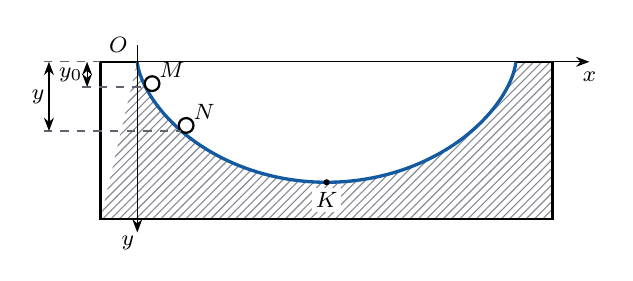
\begin{tikzpicture}[scale=0.85, >=Stealth, font=\footnotesize]
      % 摆线尺度 r = 0.90, theta in [0, 2*pi]
      \def\r{0.90}
      \pgfmathsetmacro{\w}{2*pi*\r}
      \pgfmathsetmacro{\ybot}{-2*\r - 0.55}
      \pgfmathsetmacro{\xL}{-0.55}
      \pgfmathsetmacro{\xR}{\w + 0.55}

      % M (theta0 = 0.95 rad) 与 N (theta = 1.72 rad)
      \def\tM{0.95}
      \def\tN{1.72}
      \pgfmathsetmacro{\xM}{\r*(\tM - sin(\tM r))}
      \pgfmathsetmacro{\yM}{-\r*(1 - cos(\tM r))}
      \pgfmathsetmacro{\xN}{\r*(\tN - sin(\tN r))}
      \pgfmathsetmacro{\yN}{-\r*(1 - cos(\tN r))}
      % 滚珠圆心沿内法线偏移半径 rb = 0.11
      \def\rb{0.11}
      \pgfmathsetmacro{\nxM}{cos(\tM/2 r)}
      \pgfmathsetmacro{\nyM}{sin(\tM/2 r)}
      \pgfmathsetmacro{\nxN}{cos(\tN/2 r)}
      \pgfmathsetmacro{\nyN}{sin(\tN/2 r)}

      % 钢板剖面阴影填充（摆线槽下方）
      \fill[pattern=north east lines, pattern color=mutedgray!75]
        (\xL, 0) -- (0, 0)
        plot[domain=0:{2*pi}, samples=90] ({\r*(\x - sin(\x r))}, {-\r*(1 - cos(\x r))})
        -- (\w, 0) -- (\xR, 0) -- (\xR, \ybot) -- (\xL, \ybot) -- cycle;

      % 钢板外框与摆线槽轮廓
      \draw[thick] (\xL, \ybot) rectangle (\xR, 0);
      \draw[very thick, curveblue, smooth, domain=0:{2*pi}, samples=90]
        plot ({\r*(\x - sin(\x r))}, {-\r*(1 - cos(\x r))});
      % 槽顶白底覆盖上边框线
      \draw[white, line width=1.4pt] (0.02, 0) -- ({\w - 0.02}, 0);

      % 坐标轴
      \draw[->] (\xL, 0) -- ({\xR + 0.55}, 0) node[below] {$x$};
      \draw[->] (0, 0.25) -- (0, {\ybot - 0.2}) node[below left, fill=white, inner sep=1pt] {$y$};
      \node[above left] at (0, 0) {$O$};

      % 滚珠（置于 M 和 N 处）
      \filldraw[fill=white, draw=black, thick] ({\xM + \rb*\nxM}, {\yM + \rb*\nyM}) circle (\rb);
      \filldraw[fill=white, draw=black, thick] ({\xN + \rb*\nxN}, {\yN + \rb*\nyN}) circle (\rb);
      \node[above right, inner sep=1.5pt] at ({\xM + \rb*\nxM + 0.04}, {\yM + \rb*\nyM + 0.02}) {$M$};
      \node[above right, inner sep=1.5pt] at ({\xN + \rb*\nxN + 0.04}, {\yN + \rb*\nyN + 0.02}) {$N$};

      % 最低点 K
      \fill ({\r*pi}, {-2*\r}) circle (1.3pt);
      \node[below, fill=white, inner sep=1.5pt, yshift=-2pt] at ({\r*pi}, {-2*\r}) {$K$};

      % 左侧高度标注 y0, y
      \draw[dashed, mutedgray] (-1.40, 0) -- (\xL, 0);
      \draw[dashed, mutedgray] (-0.82, \yM) -- (\xM, \yM);
      \draw[dashed, mutedgray] (-1.40, \yN) -- (\xN, \yN);
      \draw[<->, thin] (-0.75, 0) -- (-0.75, \yM) node[midway, left, inner sep=1.5pt] {$y_0$};
      \draw[<->, thin] (-1.32, 0) -- (-1.32, \yN) node[midway, left, inner sep=1.5pt] {$y$};
    \end{tikzpicture}
    \captionof*{figure}{图 15.1}
  \end{minipage}
\end{center}

摆线的等时性可证明如下。如图 15.1 选取坐标系，摆线槽的曲线方程可以写成
\[
  x = r(\theta - \sin\theta),\quad y = r(1 - \cos\theta).\quad (0 \leqslant \theta \leqslant 2\pi)
\]
摆线槽最低点 $K$ 的参数值是 $\theta = \pi$。设滚珠的初始位置 $M(x_0, y_0)$ 的参数值是 $\theta_0$，它在 $M$ 处时的速度为 $0$。又设滚珠沿摆线槽滚到 $N(x, y)$ 处时，离底面的高度下降了 $h$，那么
\begin{align*}
  h &= y - y_0 = r(1 - \cos\theta) - r(1 - \cos\theta_0) \\
    &= r(\cos\theta_0 + 1 - \cos\theta - 1) \\
    &= 2r\left(\cos^2\frac{\theta_0}{2} - \cos^2\frac{\theta}{2}\right).
\end{align*}
设滚珠的质量为 $m$，在 $N$ 处的速度大小为 $v$，由于滚珠从 $M$ 下降到 $N$ 所减少的势能 $mgh$ 全部转化成动能 $\frac{1}{2}mv^2$（我们假定滚动是无阻尼的），从而得到 $mgh = \frac{1}{2}mv^2$，即
\[
  v = \sqrt{2gh}.
\]

另一方面，速度 $v$ 等于弧长 $s$ 对时间 $t$ 的导数，所以
\begin{align*}
  v &= \frac{ds}{dt} = \frac{\sqrt{x'^2 + y'^2}\dd\theta}{dt} \\
    &= \sqrt{r^2(1 - \cos\theta)^2 + r^2\sin^2\theta}\,\frac{d\theta}{dt} \\
    &= \sqrt{2r^2(1 - \cos\theta)}\,\frac{d\theta}{dt} \\
    &= 2r\sin\frac{\theta}{2} \cdot \frac{d\theta}{dt}.
\end{align*}
综合上列各式，得到
\begin{gather*}
  \frac{2r\sin\frac{\theta}{2}\dd\theta}{dt} = \sqrt{4gr\left(\cos^2\frac{\theta_0}{2} - \cos^2\frac{\theta}{2}\right)}, \\
  \therefore\ dt = \frac{\sqrt{r}\sin\frac{\theta}{2}\dd\theta}{\sqrt{g\left(\cos^2\frac{\theta_0}{2} - \cos^2\frac{\theta}{2}\right)}}.
\end{gather*}
对于上式从 $\theta = \theta_0$ 到 $\theta = \pi$ 积分，就得到滚珠从 $M$ 滚到 $K$ 所需的时间是
\begin{align*}
  T &= \int_{\theta_0}^{\pi} \frac{\sqrt{r}\sin\frac{\theta}{2}\dd\theta}{\sqrt{g\left(\cos^2\frac{\theta_0}{2} - \cos^2\frac{\theta}{2}\right)}} \\
    &= -2\sqrt{\frac{r}{g}} \int_{\theta_0}^{\pi} \frac{d\left(\cos\frac{\theta}{2}\right)}{\sqrt{\cos^2\frac{\theta_0}{2} - \cos^2\frac{\theta}{2}}}.
\end{align*}
令 $\cos\frac{\theta_0}{2} = a$，$\cos\frac{\theta}{2} = u$，并且利用
\[
  \int \frac{du}{\sqrt{a^2 - u^2}} = \arcsin\frac{u}{a} + C,
\]
可得
\begin{align*}
  T &= \left.-2\sqrt{\frac{r}{g}}\arcsin\frac{\cos\frac{\theta}{2}}{\cos\frac{\theta_0}{2}}\right|_{\theta_0}^{\pi} \\
    &= -2\sqrt{\frac{r}{g}}(\arcsin 0 - \arcsin 1) = \pi\sqrt{\frac{r}{g}}.
\end{align*}
上面的计算结果表明，滚珠从初始位置 $M$ 下降到摆线槽最低点所用的时间是常数 $\pi\sqrt{\frac{r}{g}}$，与初始位置无关。因而不论摆动幅度大小，滚珠沿摆线槽每来回摆动一次所用的时间都是 $4\pi\sqrt{\frac{r}{g}}$。

\section{利用摆线板画摆线}
\markboth{16. 利用摆线板画摆线}{16. 利用摆线板画摆线}

如图 16.1，木板 $OAB$ 的轮廓线，在 $OA$ 部分是摆线的半拱弧，$AB$ 为拱高，用一段没有伸缩性的柔软细线绷紧在摆线弧 $\arc{OA}$ 上。

现在把线的一端固定在 $O$ 点，另一端系一个小环，用笔尖套在 $A$ 端的小环里拉紧细线，并且移动笔尖，使细线从 $A$ 端开始逐渐离开摆线板而伸直，一直到整个细线刚好完全伸直为止。这时笔尖将画出图 16.1 中虚线所示的曲线弧 $\arc{AK}$。这 $\arc{AK}$ 是一条什么曲线呢？

\begin{center}
  \begin{minipage}{\linewidth}
    \centering
    \begin{minipage}[b]{0.48\textwidth}
      \centering
      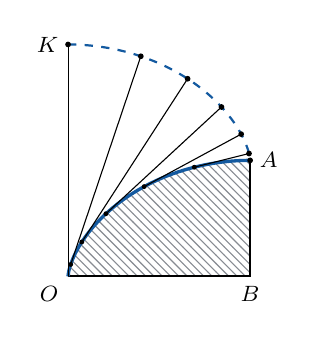
\begin{tikzpicture}[scale=0.80, >=Stealth, font=\footnotesize]
        \def\r{0.92}
        % 木板 OAB 阴影填充
        \fill[pattern=north west lines, pattern color=mutedgray!75]
          (0, 0) -- ({\r*pi}, 0) -- ({\r*pi}, {2*\r})
          plot[domain=pi:0, samples=60] ({\r*(\x - sin(\x r))}, {\r*(1 - cos(\x r))})
          -- cycle;
        % 木板轮廓
        \draw[thick] (0, 0) -- ({\r*pi}, 0) -- ({\r*pi}, {2*\r});
        \draw[very thick, curveblue, smooth, domain=0:pi, samples=60]
          plot ({\r*(\x - sin(\x r))}, {\r*(1 - cos(\x r))});

        % 渐伸线 AK（虚线）
        \draw[thick, dashed, curveblue, smooth, domain=0:pi, samples=60]
          plot ({\r*(\x + sin(\x r))}, {2*\r + \r*(1 + cos(\x r))});

        % 若干位置拉直的细线
        \draw[thin] (0, 0) -- (0, {4*\r});
        \fill (0, {4*\r}) circle (1.3pt);
        \foreach \th in {0.65, 1.15, 1.65, 2.15, 2.65} {
          \pgfmathsetmacro{\mx}{\r*(\th - sin(\th r))}
          \pgfmathsetmacro{\my}{\r*(1 - cos(\th r))}
          \pgfmathsetmacro{\nx}{\r*(\th + sin(\th r))}
          \pgfmathsetmacro{\ny}{2*\r + \r*(1 + cos(\th r))}
          \draw[thin] (\mx, \my) -- (\nx, \ny);
          \fill (\mx, \my) circle (1.1pt);
          \fill (\nx, \ny) circle (1.3pt);
        }
        \fill ({\r*pi}, {2*\r}) circle (1.3pt);

        \node[below left] at (0, 0) {$O$};
        \node[below] at ({\r*pi}, 0) {$B$};
        \node[right] at ({\r*pi}, {2*\r}) {$A$};
        \node[left] at (0, {4*\r}) {$K$};
      \end{tikzpicture}
      \captionof*{figure}{图 16.1}
    \end{minipage}\hfill
    \begin{minipage}[b]{0.48\textwidth}
      \centering
      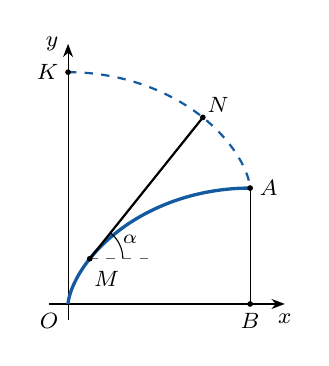
\begin{tikzpicture}[scale=0.80, >=Stealth, font=\footnotesize]
        \def\r{0.92}
        \def\th{1.35}
        \pgfmathsetmacro{\mx}{\r*(\th - sin(\th r))}
        \pgfmathsetmacro{\my}{\r*(1 - cos(\th r))}
        \pgfmathsetmacro{\nx}{\r*(\th + sin(\th r))}
        \pgfmathsetmacro{\ny}{2*\r + \r*(1 + cos(\th r))}

        % 坐标轴
        \draw[->] (-0.3, 0) -- ({\r*pi + 0.55}, 0) node[below] {$x$};
        \draw[->] (0, -0.25) -- (0, {4*\r + 0.45}) node[left] {$y$};
        \node[below left] at (0, 0) {$O$};

        % 摆线 OA 与垂线 AB
        \draw[very thick, curveblue, smooth, domain=0:pi, samples=60]
          plot ({\r*(\x - sin(\x r))}, {\r*(1 - cos(\x r))});
        \draw[thin] ({\r*pi}, 0) -- ({\r*pi}, {2*\r});

        % 渐伸线 AK（虚线）
        \draw[thick, dashed, curveblue, smooth, domain=0:pi, samples=60]
          plot ({\r*(\x + sin(\x r))}, {2*\r + \r*(1 + cos(\x r))});

        % 切线 MN 与水平线
        \coordinate (M) at (\mx, \my);
        \coordinate (N) at (\nx, \ny);
        \coordinate (H) at ({\mx + 1.0}, \my);
        \draw[thick] (M) -- (N);
        \draw[dashed, mutedgray] (M) -- (H);
        \pic[draw, angle radius=0.42cm, angle eccentricity=1.35, "\scriptsize$\alpha$"] {angle=H--M--N};

        % 点与标注
        \fill (M) circle (1.3pt) node[below right, xshift=-2pt, yshift=-1pt] {$M$};
        \fill (N) circle (1.3pt) node[above right, inner sep=1.5pt] {$N$};
        \fill ({\r*pi}, {2*\r}) circle (1.3pt) node[right] {$A$};
        \fill ({\r*pi}, 0) circle (1.3pt) node[below] {$B$};
        \fill (0, {4*\r}) circle (1.3pt) node[left] {$K$};
      \end{tikzpicture}
      \captionof*{figure}{图 16.2}
    \end{minipage}
  \end{minipage}
\end{center}

如图 16.2 选取坐标系，半拱摆线弧 $\arc{OA}$ 的方程是
\[
  x = r(\theta - \sin\theta),\quad y = r(1 - \cos\theta),
\]
其中 $0 \leqslant \theta \leqslant \pi$。设当笔尖从 $A$ 移到点 $N(X, Y)$ 时，细线被拉直的部分是 $MN$，弯曲部分是 $\arc{OM}$，这时 $M(x, y)$ 是摆线上的点，$MN$ 是摆线的切线，并且线段 $MN$ 的长度等于摆线弧 $\arc{MA}$ 的弧长 $s$。设切线 $MN$ 与 $x$ 轴的夹角为 $\alpha$，则因为 $\overrightarrow{ON} = \overrightarrow{OM} + \overrightarrow{MN}$，所以 $N$ 点的坐标为
\begin{gather*}
  X = x + MN\cos\alpha, \\
  Y = y + MN\sin\alpha,
\end{gather*}
并且
\begin{align*}
  \tg\alpha &= \frac{dy}{dx} = \frac{y'\dd\theta}{x'\dd\theta} = \frac{r\sin\theta}{r(1 - \cos\theta)} \\
            &= \ctg\frac{\theta}{2} = \tg\left(\frac{\pi}{2} - \frac{\theta}{2}\right), \\
  \therefore\ \alpha &= \frac{\pi}{2} - \frac{\theta}{2};
\end{align*}
\begin{align*}
  MN &= s = \int_{\theta}^{\pi} \sqrt{x'^2 + y'^2}\dd\theta \\
     &= \int_{\theta}^{\pi} \sqrt{r^2(1 - \cos\theta)^2 + r^2\sin^2\theta}\dd\theta \\
     &= \int_{\theta}^{\pi} 2r\sin\frac{\theta}{2}\dd\theta
      = \left.-4r\cos\frac{\theta}{2}\right|_{\theta}^{\pi} = 4r\cos\frac{\theta}{2}.
\end{align*}

综合上列各式，得到
\begin{align*}
  X &= r(\theta - \sin\theta) + 4r\cos\frac{\theta}{2}\cos\left(\frac{\pi}{2} - \frac{\theta}{2}\right) \\
    &= r(\theta - \sin\theta) + 4r\cos\frac{\theta}{2}\sin\frac{\theta}{2} \\
    &= r(\theta - \sin\theta) + 2r\sin\theta \\
    &= r(\theta + \sin\theta),
\end{align*}
\begin{align*}
  Y &= r(1 - \cos\theta) + 4r\cos\frac{\theta}{2}\sin\left(\frac{\pi}{2} - \frac{\theta}{2}\right) \\
    &= r(1 - \cos\theta) + 4r\cos^2\frac{\theta}{2} \\
    &= r(1 - \cos\theta) + 2r(1 + \cos\theta) \\
    &= 2r + r(1 + \cos\theta).
\end{align*}

下面我们来证明 $N$ 点的轨迹也是摆线。令
\[
  \theta = \theta_1 + \pi,\quad (0 \leqslant \theta \leqslant \pi)
\]
$N$ 点的坐标 $X$ 和 $Y$ 化为
\[
  X = \pi r + r(\theta_1 - \sin\theta_1),\quad Y = 2r + r(1 - \cos\theta_1).
\]
把坐标原点平移到点 $(\pi r, 2r)$（图 16.3），则点 $(X, Y)$ 在新坐标系中的坐标 $(X', Y')$ 由下式决定：

\noindent
\begin{minipage}[c]{0.42\textwidth}
  \centering
  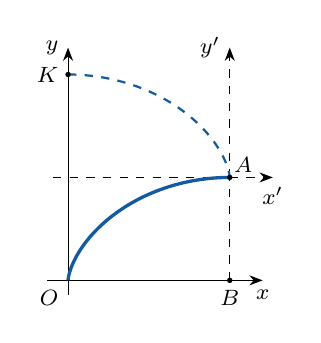
\begin{tikzpicture}[scale=0.76, >=Stealth, font=\footnotesize]
    \def\r{0.86}
    % 原坐标系
    \draw[->] (-0.35, 0) -- ({\r*pi + 0.55}, 0) node[below] {$x$};
    \draw[->] (0, -0.25) -- (0, {4*\r + 0.45}) node[left] {$y$};
    \node[below left] at (0, 0) {$O$};

    % 新坐标系（平移到 A）
    \draw[dashed] (-0.25, {2*\r}) -- ({\r*pi}, {2*\r});
    \draw[->, dashed] ({\r*pi}, {2*\r}) -- ({\r*pi + 0.72}, {2*\r}) node[below] {$x'$};
    \draw[dashed] ({\r*pi}, 0) -- ({\r*pi}, {2*\r});
    \draw[->, dashed] ({\r*pi}, {2*\r}) -- ({\r*pi}, {4*\r + 0.45}) node[left] {$y'$};

    % 曲线 OA 与 AK
    \draw[very thick, curveblue, smooth, domain=0:pi, samples=60]
      plot ({\r*(\x - sin(\x r))}, {\r*(1 - cos(\x r))});
    \draw[thick, dashed, curveblue, smooth, domain=0:pi, samples=60]
      plot ({\r*(\x + sin(\x r))}, {2*\r + \r*(1 + cos(\x r))});

    \fill ({\r*pi}, {2*\r}) circle (1.3pt) node[above right, inner sep=1.5pt] {$A$};
    \fill ({\r*pi}, 0) circle (1.3pt) node[below] {$B$};
    \fill (0, {4*\r}) circle (1.3pt) node[left] {$K$};
  \end{tikzpicture}
  \captionof*{figure}{图 16.3}
\end{minipage}\hfill
\begin{minipage}[c]{0.55\textwidth}
  \[
    X' = X - \pi r,\quad Y' = Y - 2r.
  \]
  因而曲线弧 $\arc{AK}$ 在新坐标系中的方程是
  \begin{gather*}
    X' = r(\theta_1 - \sin\theta_1), \\
    Y' = r(1 - \cos\theta_1),
  \end{gather*}
  其中 $-\pi \leqslant \theta_1 \leqslant 0$。这说明 $\arc{AK}$ 也是摆线的半拱弧，并且其拱高与原摆线 $\arc{OA}$ 的拱高相等，都是 $2r$，区别只在于 $\arc{OA}$ 是前半拱，$\arc{KA}$ 是后半拱，并且位置不同。
\end{minipage}

\section{摆线时钟}
\markboth{17. 摆线时钟}{17. 摆线时钟}

我们已经从“滚珠荡秋千”的游戏中认识到摆线的等时性，又通过“利用摆线板画摆线”的问题知道了怎样利用绷紧在摆线板上的细线画出新的摆线。把这两项知识结合起来，就可以理解著名的摆线时钟问题了。

钟摆在滴答声中来回摆动一次，每次摆动所用的时间必须严格地相等，才能保证计时的准确性。通常时钟的钟摆是把摆锤挂在摆杆上，沿圆弧来回摆动。由于各种因素的影响，钟摆每次摆动的幅度不可能保持绝对不变。而当摆锤沿圆弧摆动时，来回摆动一次所用的时间与摆动幅度有关：摆幅越小，摆动一次的时间越短。能不能设计一种钟摆，使它每摆动一次所用的时间不受摆幅大小的影响，始终保持常数呢？

\begin{wrapfigure}{r}{0.40\textwidth}
  \centering
  \vspace{-4pt}
  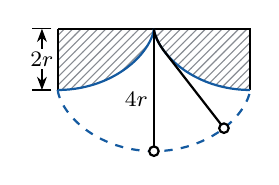
\begin{tikzpicture}[scale=0.67, >=Stealth, font=\footnotesize]
    \def\r{0.58}
    \def\th{1.32}
    \pgfmathsetmacro{\mx}{\r*(\th - sin(\th r))}
    \pgfmathsetmacro{\my}{-\r*(1 - cos(\th r))}
    \pgfmathsetmacro{\nx}{\r*(\th + sin(\th r))}
    \pgfmathsetmacro{\ny}{-2*\r - \r*(1 + cos(\th r))}

    % 左侧摆线挡板
    \fill[pattern=north east lines, pattern color=mutedgray!75]
      ({-\r*pi}, 0) -- (0, 0)
      plot[domain=0:pi, samples=50] ({-\r*(\x - sin(\x r))}, {-\r*(1 - cos(\x r))})
      -- ({-\r*pi}, 0);
    \draw[thick] ({-\r*pi}, 0) -- (0, 0);
    \draw[thick] ({-\r*pi}, 0) -- ({-\r*pi}, {-2*\r});
    \draw[thick, curveblue, smooth, domain=0:pi, samples=50]
      plot ({-\r*(\x - sin(\x r))}, {-\r*(1 - cos(\x r))});

    % 右侧摆线挡板
    \fill[pattern=north east lines, pattern color=mutedgray!75]
      (0, 0) -- ({\r*pi}, 0) -- ({\r*pi}, {-2*\r})
      plot[domain=pi:0, samples=50] ({\r*(\x - sin(\x r))}, {-\r*(1 - cos(\x r))})
      -- cycle;
    \draw[thick] (0, 0) -- ({\r*pi}, 0) -- ({\r*pi}, {-2*\r});
    \draw[thick, curveblue, smooth, domain=0:pi, samples=50]
      plot ({\r*(\x - sin(\x r))}, {-\r*(1 - cos(\x r))});

    % 左侧 2r 高度标记
    \draw[thin] ({-\r*pi - 0.12}, 0) -- ({-\r*pi - 0.48}, 0);
    \draw[thin] ({-\r*pi - 0.12}, {-2*\r}) -- ({-\r*pi - 0.48}, {-2*\r});
    \draw[<->, thin] ({-\r*pi - 0.30}, 0) -- ({-\r*pi - 0.30}, {-2*\r})
      node[midway, fill=white, inner sep=1pt] {$2r$};

    % 摆锤虚线摆线轨迹
    \draw[thick, dashed, curveblue, smooth, domain=-pi:pi, samples=80]
      plot ({\r*(\x + sin(\x r))}, {-2*\r - \r*(1 + cos(\x r))});

    % 铅垂悬线（长 4r）与最低点摆锤
    \draw[thick] (0, 0) -- (0, {-4*\r});
    \node[left, inner sep=2pt] at (0, {-2.3*\r}) {$4r$};
    \filldraw[fill=white, draw=black, thick] (0, {-4*\r}) circle (0.09);

    % 摆向右方的贴合段与切线细线与摆锤
    \draw[thick, smooth, domain=0:\th, samples=25]
      plot ({\r*(\x - sin(\x r))}, {-\r*(1 - cos(\x r))});
    \draw[thick] (\mx, \my) -- (\nx, \ny);
    \filldraw[fill=white, draw=black, thick] (\nx, \ny) circle (0.09);
  \end{tikzpicture}
  \captionof*{figure}{图 17.1}
  \vspace{-6pt}
\end{wrapfigure}
同“滚珠荡秋千”的游戏比较，滚珠相当于这里的摆锤，所以只要设法让摆锤不是沿圆弧摆动，而是沿摆线弧摆动，就能使摆动周期严格保持一定，不受摆幅变化的影响。又根据“利用摆线板画摆线”问题的答案，只要像图 17.1 那样把摆锤悬挂在长为 $4r$（摆线半拱的弧长）的能弯曲但不能伸长的细线上，悬挂点的两边各放一块摆线挡板，使挡板的曲线轮廓是拱高为 $2r$ 的半拱摆线，这样就能保证摆锤沿着图中虚线所示的摆线弧摆动。无论摆幅大小如何，摆锤沿这摆线弧来回摆动一次，所用的时间都是 $4\pi\sqrt{\frac{r}{g}}$。

十七世纪物理学家惠更斯发现了摆线的等时性以后，就用它来设计出这种巧妙的摆线时钟。“摆线”这个名称，正是由于这种曲线被应用于改进钟摆而得来的。

\clearpage

\section{短幅摆线和长幅摆线}
\markboth{18. 短幅摆线和长幅摆线}{18. 短幅摆线和长幅摆线}

当动圆 $C$ 沿着定直线 $l$ 滚动时，固定在圆 $C$ 的平面内但不在圆周上的一点 $M$ 所画出的曲线叫做变幅摆线。变幅摆线可以分成两类：当 $M$ 点固定在圆 $C$ 内部时，曲线称为短幅摆线（图 18.1，上）；当 $M$ 点在圆 $C$ 外部时，曲线称为长幅摆线，又叫做余摆线（图 18.1，下）。

设圆 $C$ 的半径是 $r$，$M$ 点到圆心 $C$ 的距离是 $a$。取定直线 $l$ 为 $x$ 轴，并使动圆位于 $x$ 轴上方。又选取原点的位置，使得当动圆的圆心移动到 $y$ 轴上时，$M$ 点运动到最低位置。

\begin{center}
  \begin{minipage}{\linewidth}
    \centering
    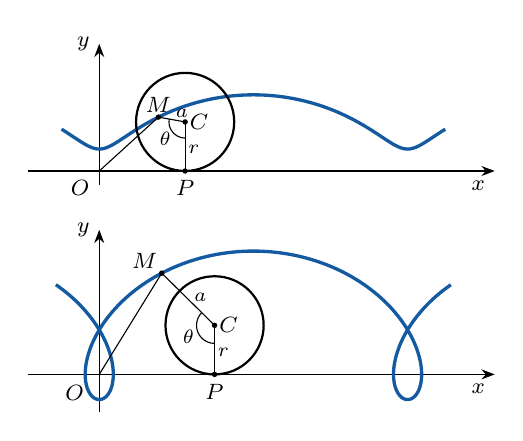
\begin{tikzpicture}[scale=0.82, >=Stealth, font=\footnotesize]
      % 上图：短幅摆线 (a < r)
      \begin{scope}[yshift=3.15cm]
        \def\r{0.76}
        \def\a{0.42}
        \def\th{1.75}
        \pgfmathsetmacro{\cx}{\r*\th}
        \pgfmathsetmacro{\cy}{\r}
        \pgfmathsetmacro{\mx}{\r*\th - \a*sin(\th r)}
        \pgfmathsetmacro{\my}{\r - \a*cos(\th r)}
        \pgfmathsetmacro{\angM}{deg(1.5*pi - \th)}

        \draw[->] (-1.1, 0) -- ({2*pi*\r + 1.35}, 0) node[below left] {$x$};
        \draw[->] (0, -0.22) -- (0, {2*\r + 0.45}) node[left] {$y$};
        \node[below left] at (0, 0) {$O$};

        \draw[very thick, curveblue, smooth, domain=-1.3:{2*pi+1.3}, samples=100]
          plot ({\r*\x - \a*sin(\x r)}, {\r - \a*cos(\x r)});

        \coordinate (O1) at (0, 0);
        \coordinate (C1) at (\cx, \cy);
        \coordinate (P1) at (\cx, 0);
        \coordinate (M1) at (\mx, \my);

        \draw[thick] (C1) circle (\r);
        \draw[thin] (O1) -- (M1);
        \draw[thin] (C1) -- (M1);
        \draw[thin] (C1) -- (P1);
        \draw (C1) ++(270:0.25) arc (270:\angM:0.25);
        \node at ($(C1)+({0.5*(270+\angM)}:0.40)$) {\scriptsize$\theta$};

        \fill (C1) circle (1.2pt) node[right, inner sep=1.5pt] {$C$};
        \fill (M1) circle (1.2pt) node[above, inner sep=1.5pt] {$M$};
        \fill (P1) circle (1.2pt) node[below] {$P$};
        \node[right, inner sep=1pt] at ($(C1)!0.55!(P1)$) {\scriptsize$r$};
        \node[above right, inner sep=0.5pt] at ($(C1)!0.42!(M1)$) {\scriptsize$a$};
      \end{scope}

      % 下图：长幅摆线 (a > r)
      \begin{scope}[yshift=0cm]
        \def\r{0.76}
        \def\a{1.15}
        \def\th{2.35}
        \pgfmathsetmacro{\cx}{\r*\th}
        \pgfmathsetmacro{\cy}{\r}
        \pgfmathsetmacro{\mx}{\r*\th - \a*sin(\th r)}
        \pgfmathsetmacro{\my}{\r - \a*cos(\th r)}
        \pgfmathsetmacro{\angM}{deg(1.5*pi - \th)}

        \draw[->] (-1.1, 0) -- ({2*pi*\r + 1.35}, 0) node[below left] {$x$};
        \draw[->] (0, -0.58) -- (0, {2*\r + 0.72}) node[left] {$y$};
        \node[below] at (-0.38, -0.02) {$O$};

        \draw[very thick, curveblue, smooth, domain=-2.15:{2*pi+2.15}, samples=130]
          plot ({\r*\x - \a*sin(\x r)}, {\r - \a*cos(\x r)});

        \coordinate (O2) at (0, 0);
        \coordinate (C2) at (\cx, \cy);
        \coordinate (P2) at (\cx, 0);
        \coordinate (M2) at (\mx, \my);

        \draw[thick] (C2) circle (\r);
        \draw[thin] (O2) -- (M2);
        \draw[thin] (C2) -- (M2);
        \draw[thin] (C2) -- (P2);
        \draw (C2) ++(270:0.28) arc (270:\angM:0.28);
        \node at ($(C2)+({0.5*(270+\angM)}:0.44)$) {\scriptsize$\theta$};

        \fill (C2) circle (1.2pt) node[right, inner sep=1.5pt] {$C$};
        \fill (M2) circle (1.2pt) node[above left, inner sep=1.5pt] {$M$};
        \fill (P2) circle (1.2pt) node[below] {$P$};
        \node[right, inner sep=1pt] at ($(C2)!0.55!(P2)$) {\scriptsize$r$};
        \node[above right, inner sep=0.5pt] at ($(C2)!0.42!(M2)$) {\scriptsize$a$};
      \end{scope}
    \end{tikzpicture}
    \captionof*{figure}{图 18.1}
  \end{minipage}
\end{center}

利用图 18.1 容易求得变幅摆线的参数方程是
\[
  x = rt - a\sin t,\quad y = r - a\cos t.
\]
当 $a < r$ 时得到短幅摆线，$a > r$ 时得到长幅摆线。又若令 $a = r$，就回到普通摆线的方程。

由于 $|\cos t| \leqslant 1$，所以当 $a < r$ 时恒有 $y > 0$，即短幅摆线与 $x$ 轴无公共点。当 $a > r$ 时 $y$ 的值可以为零，也可以为负，这意味着长幅摆线与 $x$ 轴相交，并且有一部分弧出现在 $x$ 轴下方\footnote{重排校订：原书此处误印作“$y$ 轴下方”，据上下文及参数方程 $y = r - a\cos t$ 订正为“$x$ 轴下方”。}。% 原书此处误印作“y 轴”
从图 18.1 看出，长幅摆线自己绕成许多小圈，叫做绕扣，每个绕扣都被 $x$ 轴分成上下两截，并且长幅摆线与 $x$ 轴的任何交点都在绕扣上。

在日常生活中很容易找到变幅摆线的实例。还是以自行车为例，当一个人推着自行车慢慢往前走时，旁观者就可以看到车轮钢圈内侧的彩色气门帽慢慢地描绘出一条短幅摆线。

\section{直线运动和旋转运动的合成}
\markboth{19. 直线运动和旋转运动的合成}{19. 直线运动和旋转运动的合成}

在摆线和变幅摆线的定义中，$M$ 点的运动是由两种简单运动合成的：一个是圆心 $C$ 沿着 $l$ 的一条平行线作直线运动，另一个是线段 $CM$ 绕 $C$ 点旋转。设直线运动的速度是 $u$，旋转的角速度是 $\omega$，那么由于动圆 $C$ 沿定直线 $l$ 滚动时没有滑动，这里的 $u$ 和 $\omega$ 总是满足关系式 $u = \omega r$。

在日常生活和工农业生产中，还容易看到很多物体，它们一面绕自己的旋转轴作旋转运动，一面又随着汽车、轮船、拖拉机、自行车等作直线运动。这些同时作旋转运动和直线运动的物体，促使我们考虑一个更复杂的轨迹问题：

动点 $C$ 沿直线 $m$ 匀速运动，速度为 $u$，同时有一定长线段 $CM$ 绕 $C$ 点匀速旋转，角速度为 $\omega$，求 $M$ 的轨迹。

注意，这个问题与摆线中 $M$ 点运动的区别在于直线运动的速度 $u$ 和旋转的角速度 $\omega$ 是互相独立的，并不一定满足 $u = \omega r$。通俗地讲，就是在试图形成摆线的过程中，圆 $C$ 与直线产生了滑动。

\noindent
\begin{minipage}[c]{0.43\textwidth}
  \centering
  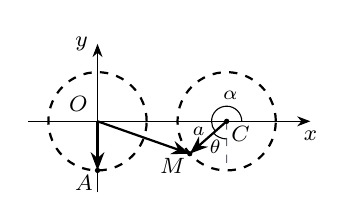
\begin{tikzpicture}[scale=0.80, >=Stealth, font=\footnotesize]
    \def\a{0.78}
    \def\cx{2.05}
    \def\th{0.85}
    \pgfmathsetmacro{\mx}{\cx - \a*sin(\th r)}
    \pgfmathsetmacro{\my}{-\a*cos(\th r)}
    \pgfmathsetmacro{\angM}{deg(1.5*pi - \th)}

    % 坐标轴
    \draw[->] (-1.1, 0) -- ({\cx + \a + 0.55}, 0) node[below] {$x$};
    \draw[->] (0, {-\a - 0.35}) -- (0, {\a + 0.45}) node[left] {$y$};
    \node[above left] at (0, 0) {$O$};

    % 两个辅助虚圆
    \draw[thick, dashed] (0, 0) circle (\a);
    \draw[thick, dashed] (\cx, 0) circle (\a);

    % 向量与辅助线段
    \coordinate (O) at (0, 0);
    \coordinate (A) at (0, -\a);
    \coordinate (C) at (\cx, 0);
    \coordinate (M) at (\mx, \my);

    \draw[->, thick] (O) -- (A);
    \draw[->, thick] (O) -- (M);
    \draw[->, thick] (C) -- (M);
    \draw[dashed, mutedgray] (C) -- (\cx, -\a);

    % 角度 theta 与 alpha
    \draw (C) ++(270:0.28) arc (270:\angM:0.28);
    \node at ($(C)+({0.5*(270+\angM)}:0.44)$) {\scriptsize$\theta$};
    \draw (C) ++(0:0.24) arc (0:\angM:0.24);
    \node at ($(C)+(82:0.42)$) {\scriptsize$\alpha$};

    \fill (A) circle (1.2pt) node[below left, inner sep=1.5pt] {$A$};
    \fill (C) circle (1.2pt) node[below right, inner sep=1.5pt] {$C$};
    \fill (M) circle (1.2pt) node[below left, inner sep=1.5pt] {$M$};
    \node[above left, inner sep=0.8pt] at ($(C)!0.52!(M)$) {\scriptsize$a$};
  \end{tikzpicture}
  \captionof*{figure}{图 19.1}
\end{minipage}\hfill
\begin{minipage}[c]{0.54\textwidth}
  \hspace*{2em}如图 19.1，选取定直线 $m$ 为 $x$ 轴，$C$ 点前进的方向为 $x$ 轴的正向，并且这样选择计算时间 $t$ 的起点：使当 $t = 0$ 时 $C$ 在原点 $O$，同时 $M$ 在 $y$ 轴的负半轴上的点 $A$ 处。记 $CM = a$。又设在时刻 $t$，向量 $\overrightarrow{OA}$ 运动到了图中 $\overrightarrow{CM}$ 的位置。这时 $OC = ut$，$\theta = \omega t$。设 $M$ 点的坐标为 $(x, y)$，则由 $\overrightarrow{OM} = \overrightarrow{OC} + \overrightarrow{CM}$ 及 $\alpha = \frac{3}{2}\pi - \theta$ 得
\end{minipage}
\begin{align*}
  (x, y) &= (ut, 0) + (CM\cos\alpha, CM\sin\alpha) \\
         &= (ut - a\sin\theta, -a\cos\theta).
\end{align*}
记 $\frac{u}{\omega} = r$（注意，这里的 $r$ 不一定等于图 19.1 中的辅助圆的半径），则 $ut = \omega rt = r\theta$，于是 $M$ 点的坐标化为
\[
  x = r\theta - a\sin\theta,\quad y = -a\cos\theta.
\]
再把 $x$ 轴向下平移 $r$（图 19.2），则点 $M$ 在新坐标系中的坐标 $(x', y')$ 为

\noindent
\begin{minipage}[c]{0.55\textwidth}
  \[
    x' = x,\quad y' = y + r,
  \]
  因而曲线方程化为
  \begin{gather*}
    x' = r\theta - a\sin\theta, \\
    y' = r - a\cos\theta.
  \end{gather*}
\end{minipage}\hfill
\begin{minipage}[c]{0.42\textwidth}
  \centering
  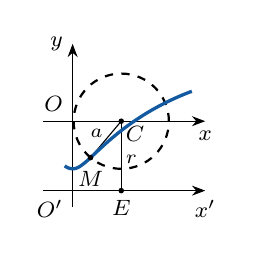
\begin{tikzpicture}[scale=0.84, >=Stealth, font=\footnotesize]
    \def\r{1.05}
    \def\a{0.72}
    \def\th{0.70}
    \pgfmathsetmacro{\cx}{\r*\th}
    \pgfmathsetmacro{\mx}{\r*\th - \a*sin(\th r)}
    \pgfmathsetmacro{\my}{-\a*cos(\th r)}

    % 坐标轴与平移后的 x' 轴
    \draw[->] (-0.45, 0) -- ({\cx + \a + 0.55}, 0) node[below] {$x$};
    \draw[->] (-0.45, -\r) -- ({\cx + \a + 0.55}, -\r) node[below] {$x'$};
    \draw[->] (0, {-\r - 0.25}) -- (0, {\a + 0.45}) node[left] {$y$};
    \node[above left] at (0, 0) {$O$};
    \node[below left] at (0, -\r) {$O'$};

    % 辅助圆与线段
    \draw[thick, dashed] (\cx, 0) circle (\a);
    \coordinate (C) at (\cx, 0);
    \coordinate (M) at (\mx, \my);
    \coordinate (E) at (\cx, -\r);
    \draw[thin] (C) -- (M);
    \draw[thin] (C) -- (E);

    % 轨迹曲线（参数方程精确绘制）
    \draw[very thick, curveblue, smooth, domain=-0.35:2.25, samples=60]
      plot ({\r*\x - \a*sin(\x r)}, {-\a*cos(\x r)});

    \fill (C) circle (1.2pt) node[below right, inner sep=1.5pt] {$C$};
    \fill (M) circle (1.2pt) node[below, yshift=-1.5pt] {$M$};
    \fill (E) circle (1.2pt) node[below] {$E$};
    \node[above left, inner sep=0.8pt] at ($(C)!0.52!(M)$) {\scriptsize$a$};
    \node[right, inner sep=1.5pt] at ($(C)!0.55!(E)$) {\scriptsize$r$};
  \end{tikzpicture}
  \captionof*{figure}{图 19.2}
\end{minipage}
从方程看出，所求的曲线仍为摆线或变幅摆线，式中 $r$ 是辅助量，定义为直线运动速度 $u$ 与旋转角速度 $\omega$ 之比。因而结论是：当 $a = \frac{u}{\omega}$ 时，轨迹是摆线；当 $a < \frac{u}{\omega}$ 时，轨迹是短幅摆线；当 $a > \frac{u}{\omega}$ 时，轨迹是长幅摆线。

\section{农业机械中的长幅摆线}
\markboth{20. 农业机械中的长幅摆线}{20. 农业机械中的长幅摆线}

很多农业机械在工作时，都有一些部件在绕着自己的轴旋转，这些部件又随着整个机具一起向前作匀速直线运动。根据第 19 节的讨论，在这些一边旋转一边前进的部件上，每个点都在空中画出一条摆线或变幅摆线。

农业机械里经常用到长幅摆线，而且主要应用它的绕扣部分。例如，图 20.1 是卧式旋耕机的工作原理示意图\footnote{重排校订：原书图 20.1 中刀片编号“1”位置不清，且四条长幅摆线轨迹起点截断参差不齐；本版重绘时将四条轨迹统一自各刀尖（$t=0$）同步出发，并清晰标出刀片 1～4。}。从图中可以看出，卧式旋耕机的每把刀片画出一条长幅摆线，它的绕扣部分很大。调整旋转轴的高度，可以使刀片在绕扣最宽的地方入土，翻松绕扣下半截的泥土后，再露出地面。四把刀片画出的四条长幅摆线顺次错开，绕扣部分互相重迭，实现了连续翻耕土地的动作。在这种机具上只有利用长幅摆线才行，如果刀尖的运动轨迹不是长幅摆线，而是普通摆线或短幅摆线，那么就不能进行翻土的动作。

\begin{center}
  \begin{tikzpicture}[scale=1.02, >=Stealth, font=\footnotesize]
    \def\r{0.26}
    \def\a{0.64}

    % 水平轴线与中心十字线
    \draw[thin] ({-\a - 0.14}, 0) -- ({3*pi*\r + \a + 0.20}, 0);
    \draw[thin] (0, {-\a - 0.14}) -- (0, {\a + 0.14});

    % 旋耕机圆盘虚线外圈
    \draw[dashed, mutedgray] (0, 0) circle (\a);

    % 四把弯刀片（1 上，2 左，3 下，4 右）
    \foreach \ang in {90, 180, 270, 0} {
      \begin{scope}[rotate=\ang]
        \draw[thick] (0, 0) .. controls ({0.35*\a}, {0.15*\a}) and ({0.65*\a}, {0.35*\a}) .. (\a, 0);
        \draw[thick] (0, 0) .. controls ({0.35*\a}, {-0.05*\a}) and ({0.72*\a}, {0.15*\a}) .. (\a, 0);
      \end{scope}
    }

    % 刀盘中心顺时针旋转弧形箭头（匹配向右行进速度 u）
    \draw[-{Stealth[length=3.6pt, width=2.6pt]}, line width=0.65pt]
      ({0.26*cos(76)}, {0.26*sin(76)}) arc[start angle=76, end angle=14, radius=0.26];

    % 前进方向 u 与刀片标注
    \draw[->] (-0.88, {\a + 0.28}) -- (-0.44, {\a + 0.28});
    \node[above, inner sep=1pt] at (-0.66, {\a + 0.29}) {$u$};
    \node[above] at (0, {\a + 0.16}) {刀片};

    % 四把刀片的长幅摆线轨迹（均从 t=0 各刀尖出发，右端统一整齐收束于最后绕扣 1 对称轴 x=3*pi*r 附近）
    % 刀片 1（90°上）：形成绕扣 1(pi), 1(3pi)，于自交点闭合
    \draw[thick, curveblue, smooth, domain=0:{3.672*pi}, samples=130]
      plot ({\r*\x + \a*sin(\x r)}, {\a*cos(\x r)});
    % 刀片 2（180°左）：形成绕扣 2(1.5pi)，于 x=3*pi*r 处与刀片 4 对称交汇
    \draw[thick, curveblue, smooth, domain=0:{2.648*pi}, samples=100]
      plot ({\r*\x + \a*sin((\x - 0.5*pi) r)}, {\a*cos((\x - 0.5*pi) r)});
    % 刀片 3（270°下）：形成绕扣 3(2pi)，于 x=3*pi*r 处到达波峰收束
    \draw[thick, curveblue, smooth, domain=0:{3.00*pi}, samples=110]
      plot ({\r*\x + \a*sin((\x - pi) r)}, {\a*cos((\x - pi) r)});
    % 刀片 4（0°右）：形成绕扣 4(0.5pi), 4(2.5pi)，于 x=3*pi*r 处与刀片 2 对称交汇
    \draw[thick, curveblue, smooth, domain=0:{3.352*pi}, samples=120]
      plot ({\r*\x + \a*sin((\x - 1.5*pi) r)}, {\a*cos((\x - 1.5*pi) r)});

    % 刀片编号 1~4 置于所有蓝色轨迹之后，加白底遮罩放于刀盘内侧干净空白处
    \node[fill=white, inner sep=0.8pt] at (0.16, 0.48) {1};
    \node[fill=white, inner sep=0.8pt] at (-0.46, 0.16) {2};
    \node[fill=white, inner sep=0.8pt] at (-0.16, -0.46) {3};
    \node[fill=white, inner sep=0.8pt] at (0.45, -0.18) {4};

    % 底部绕扣编号 4 1 2 3 4 1（与全部 6 个绕扣一一严格对应）
    \node[below] at ({\r*0.5*pi}, {-\a - 0.03}) {4};
    \node[below] at ({\r*1.0*pi}, {-\a - 0.03}) {1};
    \node[below] at ({\r*1.5*pi}, {-\a - 0.03}) {2};
    \node[below] at ({\r*2.0*pi}, {-\a - 0.03}) {3};
    \node[below] at ({\r*2.5*pi}, {-\a - 0.03}) {4};
    \node[below] at ({\r*3.0*pi}, {-\a - 0.03}) {1};
  \end{tikzpicture}
  \captionof*{figure}{图 20.1}
\end{center}

又如联合收割机的拨禾板，一面跟随联合收割机前进，一面绕自己的轴旋转。拨禾板要能沿竖直方向插入禾丛，把禾杆引向切割器，并把割断的禾杆向后推送，所以拨禾板的外端也应该描绘长幅摆线，并且在绕扣部分的下半截曲线弧上进行工作。


% --- 批次 3：第 21–30 节 ---
\section{熊猫走钢丝}
\markboth{21. 熊猫走钢丝}{21. 熊猫走钢丝}

\noindent
\begin{minipage}[c]{0.41\textwidth}
  \centering
  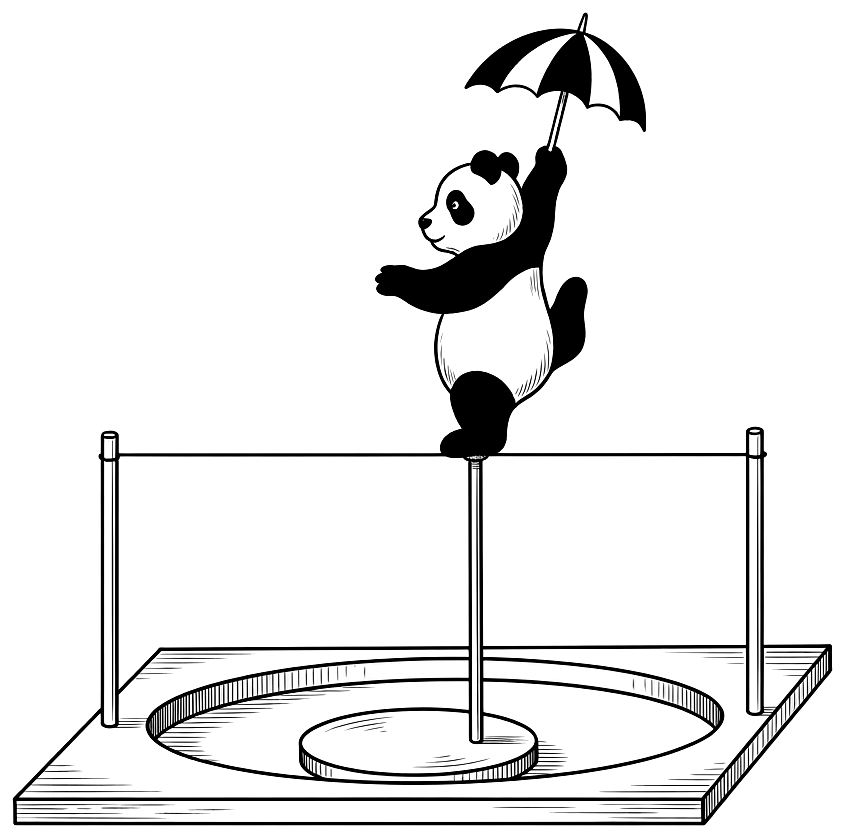
\includegraphics[width=\linewidth]{fig_021_1.png}
  \captionof*{figure}{图\ 21.1}
\end{minipage}\hfill
\begin{minipage}[c]{0.56\textwidth}
  \setlength{\parindent}{2em}\indent
  图 21.1 所画的场面，并不是马戏团表演镜头的真实写照，而只是根据数学原理设计的一个小玩具。玩具的底座上有一个圆洞，洞内有一块圆板，熊猫的模型通过细杆连接在圆板边缘上。把圆板沿圆洞边缘滚动（注意不要有滑动），就会看到细杆上端的熊猫一边沿钢丝滑动，一边还转动着肥胖的身体，非常有趣。
\end{minipage}

如果自己动手做一个这样的玩具，必须注意两个关键：第一，圆洞的直径要正好等于圆板直径的 $2$ 倍；第二，牵钢丝的两根柱子竖立在底座上的位置，应该位于圆洞的一条直径的延长线上。换句话说，钢丝在底座平面内的正射影应该是圆洞的一条直径。这个玩具的基本原理，就是下面的轨迹定理：

当半径为 $r$ 的动圆 $C$ 在半径为 $2r$ 的定圆 $O$ 内无滑动地滚动时，动圆圆周上一点 $M$ 的轨迹是圆 $O$ 的一条直径。

\noindent
\begin{minipage}[c]{0.50\textwidth}
  \setlength{\parindent}{2em}\indent
  现在证明上述事实。如图 21.2，取 $O$ 为坐标原点，并且选取 $x$ 轴，使得动圆的圆心落在 $x$ 轴正半轴上时，动圆 $C$ 上的 $M$ 点到 $O$ 的距离最远，即这时 $M(x, y)$ 将落在圆 $O$ 与 $x$ 轴正半轴的交点 $A$ 处。设动圆 $C$ 继续滚动到图中实线所示位置，这时的圆心为 $C(a, b)$，切点为 $B$，$\angle AOB=\theta$，则
\end{minipage}\hfill
\begin{minipage}[c]{0.47\textwidth}
  \centering
  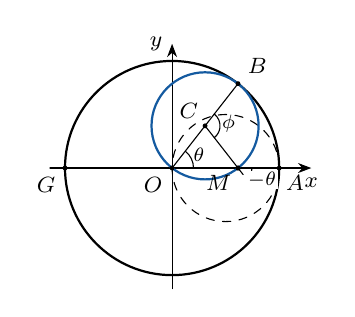
\begin{tikzpicture}[scale=0.68, >=Stealth, line cap=round, line join=round]
    \def\r{1.0}
    \def\th{52}
    \coordinate (O) at (0,0);
    \coordinate (G) at (-2*\r, 0);
    \coordinate (A) at (2*\r, 0);
    \coordinate (B) at ({2*\r*cos(\th)}, {2*\r*sin(\th)});
    \coordinate (C) at ({\r*cos(\th)}, {\r*sin(\th)});
    \coordinate (M) at ({2*\r*cos(\th)}, 0);

    % 坐标轴
    \draw[->] (-2.28, 0) -- (2.60, 0) node[below, font=\footnotesize] {$x$};
    \draw[->] (0, -2.25) -- (0, 2.32) node[left, font=\footnotesize] {$y$};

    % 定圆 O、初始位置虚线圆、动圆 C
    \draw[thick] (O) circle (2*\r);
    \draw[dashed] (\r, 0) circle (\r);
    \draw[thick, curveblue] (C) circle (\r);

    % 线段 OB, CM 及延长线
    \draw (O) -- (B);
    \draw (C) -- (M);
    \draw[thin, dashed] (M) -- ++({-\th}:0.62);

    % 角 theta, phi, -theta
    \draw (0.40, 0) arc (0:\th:0.40);
    \node[font=\scriptsize] at ({0.56*cos(0.5*\th)}, {0.56*sin(0.5*\th)}) {$\theta$};

    \draw ($(C) + (\th:0.28)$) arc (\th:{-\th}:0.28);
    \node[font=\scriptsize] at ($(C) + (0.44, 0.05)$) {$\phi$};

    \draw ($(M) + (0:0.26)$) arc (0:{-\th}:0.26);
    \node[font=\scriptsize, fill=white, inner sep=0.5pt] at ($(M) + (-26:0.50)$) {$-\theta$};

    % 关键点与标签
    \fill (O) circle (1.3pt) node[below left, font=\footnotesize] {$O$};
    \fill (G) circle (1.3pt) node[below left, font=\footnotesize] {$G$};
    \fill (A) circle (1.3pt) node[below right=-1pt, font=\footnotesize] {$A$};
    \fill (B) circle (1.3pt) node[above right, font=\footnotesize] {$B$};
    \fill (C) circle (1.3pt) node[above left=-1pt, font=\footnotesize] {$C$};
    \fill (M) circle (1.4pt) node[below left=-1pt, font=\footnotesize] {$M$};
  \end{tikzpicture}
  \captionof*{figure}{图\ 21.2}
\end{minipage}
\[
  a = r\cos\theta,\quad b = r\sin\theta.
\]

又因为滚动时没有滑动，所以小圆的 $\arc{BM}$ 与大圆的 $\arc{BA}$ 长度相等。所以，如果记 $\angle BCM=\phi$，就有
\begin{align*}
  r\phi &= (2r)\cdot\theta, \\
  \therefore\quad \phi &= 2\theta.
\end{align*}

另一方面，$\angle COM = \angle CMO = \frac{1}{2}\phi = \theta$，所以 $M$ 点必落在 $x$ 轴上，且 $\overrightarrow{CM}$ 的幅角为 $-\theta$，由 $\overrightarrow{OM} = \overrightarrow{OC} + \overrightarrow{CM}$ 得
\begin{align*}
  (x, y) &= (r\cos\theta,\, r\sin\theta) + (r\cos(-\theta),\, r\sin(-\theta)) \\
         &= (2r\cos\theta,\, 0).
\end{align*}
这样就证明了点 $M(x, y)$ 的轨迹是 $x$ 轴上的线段 $-2r\leqslant x\leqslant 2r$，即定圆 $O$ 的直径 $GA$。

\section{卡丹的转盘问题}
\markboth{22. 卡丹的转盘问题}{22. 卡丹的转盘问题}

意大利数学家卡丹（1501～1576）曾经提出如下的转盘问题：当一个圆盘沿着一个半径是它的两倍的圆盘内壁无滑动地旋转时，小圆盘上一点画出怎样的图形？

根据第 21 节的讨论，我们可以知道，小圆盘边缘上任一点的轨迹是大圆盘的一条直径。现在进而证明，小圆盘内部任一点的轨迹是一个椭圆。

\noindent
\begin{minipage}[c]{0.42\textwidth}
  \centering
  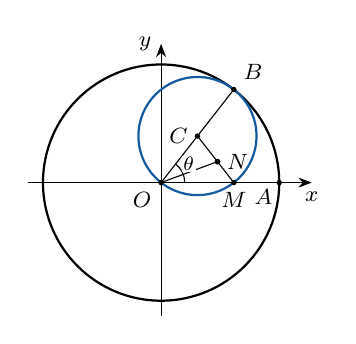
\begin{tikzpicture}[scale=0.75, >=Stealth, line cap=round, line join=round]
    % 参数 r = 1.0, 定圆半径 2r = 2.0, theta = 52 deg, h = 0.55
    \def\r{1.0}
    \def\th{52}
    \def\h{0.55}
    \coordinate (O) at (0,0);
    \coordinate (A) at (2*\r, 0);
    \coordinate (B) at ({2*\r*cos(\th)}, {2*\r*sin(\th)});
    \coordinate (C) at ({\r*cos(\th)}, {\r*sin(\th)});
    \coordinate (M) at ({2*\r*cos(\th)}, 0);
    \coordinate (N) at ({\r*cos(\th) + \h*cos(-\th)}, {\r*sin(\th) + \h*sin(-\th)});

    % 坐标轴
    \draw[->] (-2.25, 0) -- (2.55, 0) node[below, font=\footnotesize] {$x$};
    \draw[->] (0, -2.25) -- (0, 2.35) node[left, font=\footnotesize] {$y$};

    % 定圆 O 与动圆 C
    \draw[thick] (O) circle (2*\r);
    \draw[thick, curveblue] (C) circle (\r);

    % 辅助线段
    \draw (O) -- (B);
    \draw (C) -- (M);
    \draw (O) -- (N);

    % 角度标注 theta
    \draw (0.40, 0) arc (0:\th:0.40);
    \node[font=\scriptsize, fill=white, inner sep=0.5pt] at ({0.56*cos(0.65*\th)}, {0.56*sin(0.65*\th)}) {$\theta$};

    % 关键点与标签
    \fill (O) circle (1.3pt) node[below left, font=\footnotesize] {$O$};
    \fill (A) circle (1.3pt) node[below left=-1pt, font=\footnotesize] {$A$};
    \fill (B) circle (1.3pt) node[above right, font=\footnotesize] {$B$};
    \fill (C) circle (1.3pt) node[left, font=\footnotesize] {$C$};
    \fill (M) circle (1.3pt) node[below, font=\footnotesize] {$M$};
    \fill (N) circle (1.4pt) node[right, font=\footnotesize] {$N$};
  \end{tikzpicture}
  \captionof*{figure}{图\ 22.1}
\end{minipage}
\hfill
\begin{minipage}[c]{0.55\textwidth}
  \setlength{\parindent}{2em}\indent
  如图 22.1，设动圆 $C$ 的半径是 $r$，定圆 $O$ 的半径是 $2r$，$N$ 是圆 $C$ 内部与圆 $C$ 固定连结的点，$CN=h$，射线 $CN$ 交圆 $C$ 于 $M$。设在圆 $C$ 滚动的某一瞬间，$M$ 落到圆 $O$ 上的 $A$ 点，取 $OA$ 为 $x$ 轴正方向，$O$ 为原点。当圆 $C$ 继续滚动到图中位置时，由 21 节知，$\overrightarrow{CN}$ 的幅角为 $-\theta$，所以由 $\overrightarrow{ON}=\overrightarrow{OC}+\overrightarrow{CN}$ 可得向量 $\overrightarrow{ON}$ 的坐标表示式为：
\end{minipage}
\begin{align*}
  (x, y) &= (r\cos\theta,\, r\sin\theta) + (h\cos(-\theta),\, h\sin(-\theta)) \\
         &= ((r+h)\cos\theta,\, (r-h)\sin\theta)
\end{align*}
所以 $N$ 点的坐标为
\begin{align*}
  x &= (r+h)\cos\theta, \\
  y &= (r-h)\sin\theta.
\end{align*}

由于点 $N$ 在圆 $C$ 内部，所以 $h<r$，可从上式消去 $\theta$，得到
\[
  \frac{x^2}{(r+h)^2} + \frac{y^2}{(r-h)^2} = 1,
\]
这说明 $N$ 的轨迹是一个椭圆。

顺便看出，若 $N$ 在圆 $C$ 外部，即 $h>r$，则上列推理全部适用，最后得到 $N$ 的轨迹仍为椭圆，其方程为
\[
  \frac{x^2}{(h+r)^2} + \frac{y^2}{(h-r)^2} = 1.
\]

由于卡丹的转盘问题主要研究两个圆，其中的小圆在大圆内部无滑动地滚动，并且大圆半径恰好是小圆半径的两倍，所以有时也把这样的一对圆叫做卡丹圆偶。

\section{机器的“护身符”}
\markboth{23. 机器的“护身符”}{23. 机器的“护身符”}

卡丹圆偶可以使转动变成往返直线运动，而且从 $x=2r\cos\theta$ 看出，这种往返直线运动是遵循余弦规律的。这一特点可应用于机械设计。

我们知道对于沿一线段 $AG$ 作往返直线运动的物体，在它到达行程的端点 $A$ 或 $G$ 时，速度要改变方向，因而产生撞击力。在端点的速度越大，撞击力越强。特别是当机器运转很快时，这种撞击力的影响尤其明显，可以造成机器的某些部件迅速损坏。所以在设计机器时，对于作往返直线运动的部件，尤其是高速运动的部件，常需设法使它在行程端点的速度尽量小些，最好在端点的速度为零。

对于由卡丹圆偶产生的往返直线运动，位移规律是
\[
  x = 2r\cos\omega t,
\]
这里 $t$ 是时间，$\omega = \dfrac{\theta}{t}$ 是动圆圆心 $C$ 绕定圆圆心 $O$ 旋转的角速度。现在我们来看看它是否能满足上述要求。

将上式对 $t$ 求导两次，顺次得到在时刻 $t$ 的速度 $v$ 和加速度 $a$ 分别是
\begin{align*}
  v &= x' = -2r\omega\sin\omega t, \\
  a &= v' = -2r\omega^2\cos\omega t.
\end{align*}

在行程的中点处 $x=0$，因而 $\cos\omega t=0$，$\sin\omega t=\pm 1$，这时 $a=0$，$|v|$ 最大。随着动点逐渐向行程端点移动，$\cos\omega t$ 的绝对值逐渐增大，$\sin\omega t$ 的绝对值逐渐减小，因而速度 $v$ 逐渐减慢。直到到达行程端点时，$x=\pm 2r$，$\cos\omega t=\pm 1$，因而 $\sin\omega t=0$，$v=0$。这时加速度最大，速度为零，因而使撞击力大大削弱。由此看来，这“$\cos$”还是机器的“护身符”呢。

在机械设计中有很多种获得按余弦规律作往返直线运动的方法，利用卡丹圆偶只是其中的一种方法。

\section{内摆线}
\markboth{24. 内摆线}{24. 内摆线}

已知半径为 $R$ 的定圆 $O$ 和半径为 $r$ 的动圆 $O_1$，这里 $r<R$。当圆 $O_1$ 在圆 $O$ 内无滑动地滚动时，圆 $O_1$ 上一点 $M$ 的轨迹叫做内摆线。

\noindent
\begin{minipage}[c]{0.54\textwidth}
  \setlength{\parindent}{2em}\indent
  现在推导内摆线的方程。如图 24.1，选取直角坐标系，使定圆的圆心 $O$ 为原点，并且使圆 $O$ 与 $x$ 轴正半轴的交点 $A$ 是轨迹上的一点。当圆 $O_1$ 滚动到图中的任意位置时，点 $M$ 从初始位置 $A(R, 0)$ 移到位置 $(x, y)$。设这时两圆接触点为 $N$，则因为 $r<R$，点 $O_1$ 必在线段 $ON$ 上。记 $\angle NO_1M=t$，则大圆的 $\arc{NA}$ 和小圆的 $\arc{NM}$ 的长度都是 $rt$。$\angle AON = \frac{rt}{R}$，$\overrightarrow{O_1M}$ 的幅角 $\alpha = \frac{r}{R}t - t$，由 $\overrightarrow{OM} = \overrightarrow{OO_1} + \overrightarrow{O_1M}$，得到向量 $\overrightarrow{OM}$ 的坐标表示式为
\end{minipage}
\hfill
\begin{minipage}[c]{0.43\textwidth}
  \centering
  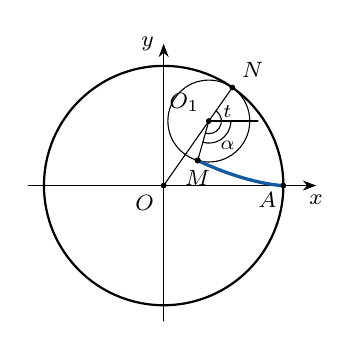
\begin{tikzpicture}[scale=0.80, >=Stealth, line cap=round, line join=round]
    % R = 1.9, r = 0.65, angle(AON) = 55 deg => t = (R/r)*55 = 160.77 deg
    \def\R{1.9}
    \def\r{0.65}
    \def\angAON{55}
    \pgfmathsetmacro{\tdeg}{\R/\r*\angAON}
    \pgfmathsetmacro{\alp}{\angAON - \tdeg}
    \coordinate (O) at (0,0);
    \coordinate (A) at (\R, 0);
    \coordinate (N) at ({\R*cos(\angAON)}, {\R*sin(\angAON)});
    \coordinate (O1) at ({(\R-\r)*cos(\angAON)}, {(\R-\r)*sin(\angAON)});
    \coordinate (M) at ({(\R-\r)*cos(\angAON) + \r*cos(\alp)}, {(\R-\r)*sin(\angAON) + \r*sin(\alp)});

    % 坐标轴
    \draw[->] (-2.15, 0) -- (2.42, 0) node[below, font=\footnotesize] {$x$};
    \draw[->] (0, -2.15) -- (0, 2.25) node[left, font=\footnotesize] {$y$};

    % 定圆与动圆
    \draw[thick] (O) circle (\R);
    \draw (O1) circle (\r);

    % 轨迹弧 AM (精确参数方程)
    \draw[very thick, curveblue, domain=0:\tdeg, samples=80, variable=\s]
      plot ({(\R-\r)*cos(\r/\R*\s) + \r*cos(\s - \r/\R*\s)},
            {(\R-\r)*sin(\r/\R*\s) - \r*sin(\s - \r/\R*\s)});

    % 辅助线段与角度
    \draw (O) -- (N);
    \draw (O1) -- (M);
    \draw[thin] (O1) -- ++(0.78, 0);

    % 角 t (从 O1N 顺时针到 O1M)
    \draw ($(O1) + (\angAON:0.20)$) arc (\angAON:\alp:0.20);
    \node[font=\scriptsize] at ($(O1) + (27:0.33)$) {$t$};

    % 角 alpha (从水平右射线顺时针到 O1M)
    \draw ($(O1) + (0:0.35)$) arc (0:\alp:0.35);
    \node[font=\scriptsize] at ($(O1) + ({0.5*\alp}:0.49)$) {$\alpha$};

    % 关键点与标签
    \fill (O) circle (1.3pt) node[below left, font=\footnotesize] {$O$};
    \fill (A) circle (1.3pt) node[below left=-1pt, font=\footnotesize] {$A$};
    \fill (N) circle (1.3pt) node[above right, font=\footnotesize] {$N$};
    \fill (O1) circle (1.3pt) node[above left, font=\footnotesize] {$O_1$};
    \fill (M) circle (1.4pt) node[below, font=\footnotesize] {$M$};
  \end{tikzpicture}
  \captionof*{figure}{图\ 24.1}
\end{minipage}
\begin{align*}
  (x, y) &= \bigl((R-r)\cos\angle AON,\, (R-r)\sin\angle AON\bigr) \\
         &\quad + (r\cos\alpha,\, r\sin\alpha) \\
         &= \biggl((R-r)\cos\frac{r}{R}t + r\cos\Bigl(t - \frac{r}{R}t\Bigr), \\
         &\qquad\ (R-r)\sin\frac{r}{R}t - r\sin\Bigl(t - \frac{r}{R}t\Bigr)\biggr)
\end{align*}
令 $\frac{r}{R}=m$，就得到内摆线的参数方程是
\[
  \begin{aligned}
    x &= (R-mR)\cos mt + mR\cos(t-mt), \\
    y &= (R-mR)\sin mt - mR\sin(t-mt).
  \end{aligned}
  \quad (0<m<1)
\]

当 $m$ 取 $0$ 与 $1$ 之间的不同数值时，可以得到各种不同形状的内摆线。图 24.2 画出了其中的几种情形\footnote{重排校订：原书图 24.2 中 $m=\frac{2}{3}$ 一图误绘为带三个绕扣的闭合圆环；按内摆线参数方程（半径比 $m=\frac{r}{R}=\frac{2}{3}$），动圆滚过三周闭合，轨迹实为与 $m=\frac{1}{3}$ 同构的三尖内摆线（三尖瓣线，有三个尖点而无绕扣），本版据正确数学方程重绘。}。图中 $m=\frac{1}{2}$ 的情形在第 21 节已详细讨论过。

\begin{figure}[htbp]
  \centering
  \begin{minipage}[t]{0.42\textwidth}
    \centering
    {\footnotesize $m=\dfrac{1}{4}$}\\[2pt]
    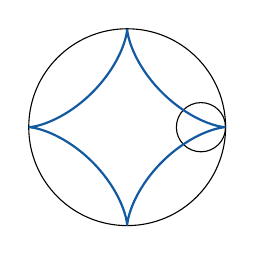
\begin{tikzpicture}[scale=1.25]
      \draw (0,0) circle (1);
      \draw (0.75, 0) circle (0.25);
      \draw[thick, curveblue, domain=0:1440, samples=200, variable=\t]
        plot ({0.75*cos(0.25*\t) + 0.25*cos(0.75*\t)},
              {0.75*sin(0.25*\t) - 0.25*sin(0.75*\t)});
    \end{tikzpicture}
  \end{minipage}
  \hspace{6mm}
  \begin{minipage}[t]{0.42\textwidth}
    \centering
    {\footnotesize $m=\dfrac{2}{5}$}\\[2pt]
    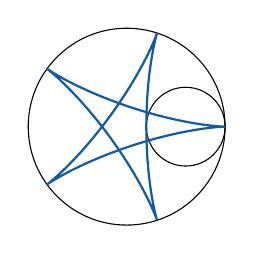
\begin{tikzpicture}[scale=1.25]
      \draw (0,0) circle (1);
      \draw (0.6, 0) circle (0.4);
      \draw[thick, curveblue, domain=0:1800, samples=260, variable=\t]
        plot ({0.6*cos(0.4*\t) + 0.4*cos(0.6*\t)},
              {0.6*sin(0.4*\t) - 0.4*sin(0.6*\t)});
    \end{tikzpicture}
  \end{minipage}

  \vspace{4mm}

  \begin{minipage}[t]{0.42\textwidth}
    \centering
    {\footnotesize $m=\dfrac{1}{2}$}\\[2pt]
    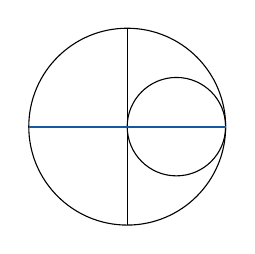
\begin{tikzpicture}[scale=1.25]
      \draw (0,0) circle (1);
      \draw (0.5, 0) circle (0.5);
      \draw (0, -1) -- (0, 1);
      \draw[thick, curveblue] (-1, 0) -- (1, 0);
    \end{tikzpicture}
  \end{minipage}
  \hspace{6mm}
  \begin{minipage}[t]{0.42\textwidth}
    \centering
    {\footnotesize $m=\dfrac{2}{3}$}\\[2pt]
    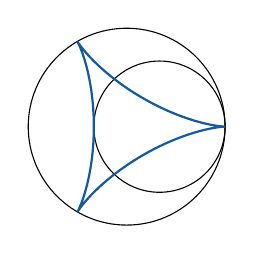
\begin{tikzpicture}[scale=1.25]
      \draw (0,0) circle (1);
      \draw (0.3333, 0) circle (0.6667);
      \draw[thick, curveblue, domain=0:1080, samples=220, variable=\t]
        plot ({0.3333*cos(0.6667*\t) + 0.6667*cos(0.3333*\t)},
              {0.3333*sin(0.6667*\t) - 0.6667*sin(0.3333*\t)});
    \end{tikzpicture}
  \end{minipage}
  \caption*{图\ 24.2}
\end{figure}

\section{曲线之星}
\markboth{25. 曲线之星}{25. 曲线之星}

当 $r=\frac{1}{4}R$ 时的内摆线有四个尖角，如图 25.1，像夜空中一颗光芒四射的星，因此叫做星形线。

\begin{figure}[htbp]
  \centering
  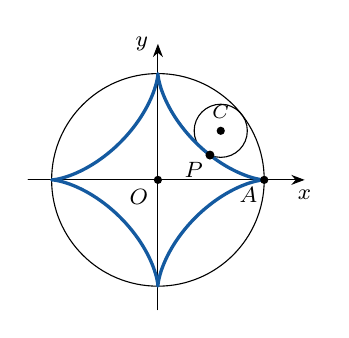
\begin{tikzpicture}[scale=1.35, >=Stealth, line cap=round, line join=round]
    \def\R{1.0}
    \def\phi{38}
    \coordinate (O) at (0,0);
    \coordinate (A) at (\R, 0);
    \coordinate (C) at ({0.75*\R*cos(\phi)}, {0.75*\R*sin(\phi)});
    \coordinate (P) at ({\R*(cos(\phi))^3}, {\R*(sin(\phi))^3});

    \draw[->] (-1.22, 0) -- (1.38, 0) node[below, font=\footnotesize] {$x$};
    \draw[->] (0, -1.22) -- (0, 1.28) node[left, font=\footnotesize] {$y$};

    \draw (O) circle (\R);
    \draw (C) circle (0.25*\R);

    \draw[very thick, curveblue, domain=0:360, samples=200, variable=\u]
      plot ({\R*(cos(\u))^3}, {\R*(sin(\u))^3});

    \fill (O) circle (1.1pt) node[below left, font=\footnotesize] {$O$};
    \fill (A) circle (1.1pt) node[below left=-1pt, font=\footnotesize] {$A$};
    \fill (C) circle (1.1pt) node[above=1pt, font=\scriptsize] {$C$};
    \fill (P) circle (1.2pt) node[below left=-1pt, font=\footnotesize] {$P$};
  \end{tikzpicture}
  \caption*{图\ 25.1}
\end{figure}

根据第 24 节，内摆线的参数方程是
\begin{align*}
  x &= (R-mR)\cos mt + mR\cos(t-mt), \\
  y &= (R-mR)\sin mt - mR\sin(t-mt),
\end{align*}
其中 $m=\frac{r}{R}$。以 $m=\frac{1}{4}$ 代入，就得到星形线的参数方程
\begin{align*}
  x &= \frac{3}{4}R\cos\frac{t}{4} + \frac{R}{4}\cos\frac{3t}{4}, \\
  y &= \frac{3}{4}R\sin\frac{t}{4} - \frac{R}{4}\sin\frac{3t}{4}.
\end{align*}
令 $t=4\varphi$，并且利用三倍角公式
\begin{align*}
  \cos 3\varphi &= 4\cos^3\varphi - 3\cos\varphi, \\
  \sin 3\varphi &= 3\sin\varphi - 4\sin^3\varphi,
\end{align*}
可将星形线的参数方程简化成
\[
  x = R\cos^3\varphi,\quad y = R\sin^3\varphi.
\]

由此又可消去参数 $\varphi$，得到星形线的直角坐标方程
\[
  x^{\frac{2}{3}} + y^{\frac{2}{3}} = R^{\frac{2}{3}}.
\]

设星形线在任意点 $P(x, y)$ 的切线斜率为 $k$，则
\[
  k = \frac{\dd y}{\dd x} = \frac{y'\dd\varphi}{x'\dd\varphi} = \frac{3R\cos\varphi\sin^2\varphi}{-3R\sin\varphi\cos^2\varphi} = -\tg\varphi.
\]
利用点斜式写出过 $P$ 的切线的方程，得到
\[
  Y - R\sin^3\varphi = -\tg\varphi\,(X - R\cos^3\varphi),
\]
这里 $X$、$Y$ 是切线上任意点的坐标。化简得
\[
  X\tg\varphi + Y = R\sin\varphi.
\]
两边同除以 $R\sin\varphi$，化为截距式
\[
  \frac{X}{R\cos\varphi} + \frac{Y}{R\sin\varphi} = 1.
\]
由此知道切线在两个坐标轴上的截距分别是
\[
  p = R\cos\varphi,\quad q = R\sin\varphi.
\]
因而切线夹在两坐标轴间的线段长为
\[
  d = \sqrt{p^2+q^2} = \sqrt{(R\cos\varphi)^2 + (R\sin\varphi)^2} = R.
\]

这样就证明了，星形线 $x=R\cos^3\varphi$，$y=R\sin^3\varphi$ 的任意切线夹在两坐标轴间的线段等于定长 $R$。由此可得到星形线的一种简便画法：

\noindent
\begin{minipage}[c]{0.42\textwidth}
  \centering
  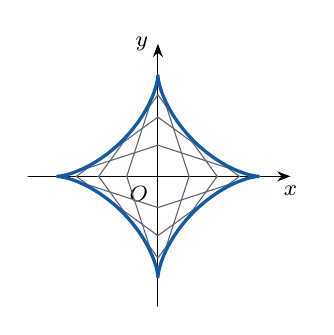
\begin{tikzpicture}[scale=1.22, >=Stealth, line cap=round, line join=round]
    \def\R{1.05}
    \draw[->] (-1.35, 0) -- (1.38, 0) node[below, font=\footnotesize] {$x$};
    \draw[->] (0, -1.35) -- (0, 1.38) node[left, font=\footnotesize] {$y$};
    \node[below left, font=\footnotesize] at (0,0) {$O$};

    % 四个象限的等长切线段族
    \foreach \ang in {18, 36, 54, 72} {
      \draw[thin, mutedgray] ({\R*cos(\ang)}, 0) -- (0, {\R*sin(\ang)});
      \draw[thin, mutedgray] ({-\R*cos(\ang)}, 0) -- (0, {\R*sin(\ang)});
      \draw[thin, mutedgray] ({-\R*cos(\ang)}, 0) -- (0, {-\R*sin(\ang)});
      \draw[thin, mutedgray] ({\R*cos(\ang)}, 0) -- (0, {-\R*sin(\ang)});
    }

    % 包络星形线
    \draw[very thick, curveblue, domain=0:360, samples=200, variable=\u]
      plot ({\R*(cos(\u))^3}, {\R*(sin(\u))^3});
  \end{tikzpicture}
  \captionof*{figure}{图\ 25.2}
\end{minipage}
\hfill
\begin{minipage}[c]{0.55\textwidth}
  \setlength{\parindent}{2em}\indent
  如图 25.2，任意作若干条长度为 $R$ 的线段，使它们的两端分别在 $x$ 轴和 $y$ 轴上；然后在每个象限里画一段光滑曲线弧，使它们与这些线段相切，就得到所要画的星形线。

  如果一条曲线弧与一族直线中的每条直线都相切，并且曲线弧上每一点都是一个切点，就说这曲线弧是这族直线的包络。本书第 1、2、8、9 节画出的抛物线和椭圆，以及图 25.2 所画出的星形线，都是某一直线族的包络。
\end{minipage}

\section{公共汽车的门与星形线}
\markboth{26. 公共汽车的门与星形线}{26. 公共汽车的门与星形线}

\noindent
\begin{minipage}[c]{0.55\textwidth}
  \setlength{\parindent}{2em}\indent
  普通房门是完整的一扇，大门是对开的两扇，唯有公共汽车的门最特殊：它不但是对开的两扇，而且每一扇都由相同的两半用铰链铰接而成。开门和关门时，靠门轴的半扇绕着门轴旋转，另外半扇的外端沿着连接两个门轴的滑槽滑动。开门时一扇车门折拢成为半扇，关门时又重新伸展成为一扇。
\end{minipage}
\hfill
\begin{minipage}[c]{0.42\textwidth}
  \centering
  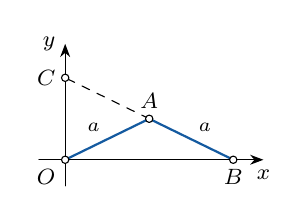
\begin{tikzpicture}[scale=0.95, >=Stealth, line cap=round, line join=round]
    \def\a{1.25}
    \def\ang{26}
    \coordinate (O) at (0,0);
    \coordinate (A) at ({\a*cos(\ang)}, {\a*sin(\ang)});
    \coordinate (B) at ({2*\a*cos(\ang)}, 0);
    \coordinate (C) at (0, {2*\a*sin(\ang)});

    \draw[->] (-0.35, 0) -- (2.65, 0) node[below, font=\footnotesize] {$x$};
    \draw[->] (0, -0.35) -- (0, 1.55) node[left, font=\footnotesize] {$y$};

    \draw[thick, curveblue] (O) -- (A) node[midway, above left=-1pt, font=\scriptsize, text=black] {$a$}
                           -- (B) node[midway, above right=-1pt, font=\scriptsize, text=black] {$a$};
    \draw[dashed] (A) -- (C);

    \fill[white] (O) circle (1.4pt); \draw (O) circle (1.4pt) node[below left, font=\footnotesize] {$O$};
    \fill[white] (A) circle (1.4pt); \draw (A) circle (1.4pt) node[above, font=\footnotesize] {$A$};
    \fill[white] (B) circle (1.4pt); \draw (B) circle (1.4pt) node[below, font=\footnotesize] {$B$};
    \fill[white] (C) circle (1.4pt); \draw (C) circle (1.4pt) node[left, font=\footnotesize] {$C$};
  \end{tikzpicture}
  \captionof*{figure}{图\ 26.1}
\end{minipage}

公共汽车采用这种折迭式的车门，有一个明显的优点，就是车门开、关所需的活动范围比较小，因而在乘车高峰时能够多载运乘客。要计算采用折迭式车门究竟节省多少地方，就必须同星形线打交道了。

如图 26.1，设折线 $OAB$ 是一扇折迭式车门，$O$ 是门轴，$OA=AB=a$。取 $O$ 为坐标原点，滑槽 $OB$ 为 $x$ 轴，延长 $BA$ 交 $y$ 轴于 $C$。在 $\triangle AOB$ 中，$AO=AB$，所以 $\angle AOB=\angle B$。又因为 $\angle BOC$ 是直角，所以 $\triangle BOC$ 是直角三角形，由此推出
\[
  \angle AOC = 90^\circ - \angle AOB = 90^\circ - \angle B = \angle C,
\]
所以从 $\triangle AOC$ 得到 $AC=AO=a$，因而
\[
  CB = 2a.\quad \text{（定长）}
\]

根据第 25 节星形线的画法，当定长线段 $BC$ 的两端分别沿 $x$ 轴和 $y$ 轴滑动时，其一切位置的包络是星形线
\[
  x = 2a\cos^3\varphi,\quad y = 2a\sin^3\varphi.
\]

\begin{figure}[htbp]
  \centering
  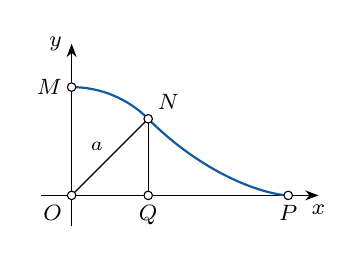
\begin{tikzpicture}[scale=1.1, >=Stealth, line cap=round, line join=round]
    \def\a{1.25}
    \coordinate (O) at (0,0);
    \coordinate (M) at (0, \a);
    \coordinate (N) at ({0.7071*\a}, {0.7071*\a});
    \coordinate (Q) at ({0.7071*\a}, 0);
    \coordinate (P) at ({2*\a}, 0);

    \draw[->] (-0.35, 0) -- (2.85, 0) node[below, font=\footnotesize] {$x$};
    \draw[->] (0, -0.35) -- (0, 1.75) node[left, font=\footnotesize] {$y$};

    % 圆弧 MN 与星形线弧 NP
    \draw[thick, curveblue] (M) arc (90:45:\a);
    \draw[thick, curveblue, domain=45:0, samples=80, variable=\u]
      plot ({2*\a*(cos(\u))^3}, {2*\a*(sin(\u))^3});

    % 辅助线 ON, NQ
    \draw (O) -- (N) node[midway, above left=-1pt, font=\scriptsize] {$a$};
    \draw (N) -- (Q);

    \fill[white] (O) circle (1.4pt); \draw (O) circle (1.4pt) node[below left, font=\footnotesize] {$O$};
    \fill[white] (M) circle (1.4pt); \draw (M) circle (1.4pt) node[left, font=\footnotesize] {$M$};
    \fill[white] (N) circle (1.4pt); \draw (N) circle (1.4pt) node[above right, font=\footnotesize] {$N$};
    \fill[white] (Q) circle (1.4pt); \draw (Q) circle (1.4pt) node[below, font=\footnotesize] {$Q$};
    \fill[white] (P) circle (1.4pt); \draw (P) circle (1.4pt) node[below, font=\footnotesize] {$P$};
  \end{tikzpicture}
  \caption*{图\ 26.2}
\end{figure}

由于车门只在第一象限活动，所以动线段 $BC$ 的包络只是这个星形线位于第一象限内的一段。这段弧又被第一象限的分角线分成上下两部分，根据对称性，半截车门 $AB$ 活动时的包络只是这星形线弧的下半部分。

由此知道，一扇折迭式车门所需要的活动范围，在水平面内的投影，是由图 26.2 中的圆弧 $\arc{MN}$、星形线弧 $\arc{NP}$ 和坐标轴围成的区域。这个区域可以划分成三个较简单的部分：扇形 $OMN$、等腰直角三角形 $OQN$ 和曲边三角形 $QNP$。把这三部分的面积顺次记成 $S_1$、$S_2$、$S_3$，三部分面积的和记成 $S$。由于 $ON=a$，$\angle MON=45^\circ$，容易得到
\[
  S_1 = \frac{1}{8}\pi a^2,\quad S_2 = \frac{1}{2}\biggl(\frac{\sqrt{2}}{2}a\biggr)^2 = \frac{1}{4}a^2.
\]

星形线弧 $\arc{NP}$ 的两个端点的坐标是 $N\Bigl(\dfrac{\sqrt{2}}{2}a,\, \dfrac{\sqrt{2}}{2}a\Bigr)$，$P(2a, 0)$。代入星形线的方程
\[
  x = 2a\cos^3\varphi,\quad y = 2a\sin^3\varphi,
\]
求得点 $N$ 的参数值是 $\varphi = \dfrac{\pi}{4}$，$P$ 的参数值是 $\varphi = 0$。所以
\begin{align*}
  S_3 &= \int_{\frac{\sqrt{2}}{2}a}^{2a} y\dd x \\
      &= \int_{\frac{\pi}{4}}^{0} 2a\sin^3\varphi \cdot (-6a)\cos^2\varphi\sin\varphi\dd\varphi \\
      &= 12a^2\int_{0}^{\frac{\pi}{4}} \sin^4\varphi\cos^2\varphi\dd\varphi \\
      &= 3a^2\int_{0}^{\frac{\pi}{4}} \sin^2 2\varphi \sin^2\varphi\dd\varphi \\
      &= \frac{3}{2}a^2\int_{0}^{\frac{\pi}{4}} \sin^2 2\varphi\,(1-\cos 2\varphi)\dd\varphi \\
      &= \frac{3}{2}a^2\biggl[\int_{0}^{\frac{\pi}{4}} \frac{1-\cos 4\varphi}{2}\dd\varphi \\
      &\qquad\qquad - \frac{1}{2}\int_{0}^{\frac{\pi}{4}} \sin^2 2\varphi\dd(\sin 2\varphi)\biggr] \\
      &= \frac{3}{2}a^2\biggl[\frac{1}{2}\varphi - \frac{1}{8}\sin 4\varphi
         - \frac{1}{2}\cdot\frac{\sin^3 2\varphi}{3}\biggr]\biggr|_{0}^{\frac{\pi}{4}} \\
      &= \frac{3}{2}a^2\biggl[\frac{\pi}{8} - \frac{1}{6}\biggr]
       = \frac{3}{16}\pi a^2 - \frac{1}{4}a^2
\end{align*}
\begin{align*}
  \therefore\quad S &= S_1 + S_2 + S_3 \\
                    &= \frac{1}{8}\pi a^2 + \frac{1}{4}a^2 + \biggl(\frac{3}{16}\pi a^2 - \frac{1}{4}a^2\biggr) \\
                    &= \frac{5}{16}\pi a^2.
\end{align*}

这就是说，一扇总宽度为 $2a$ 的折迭式车门，所需的活动面积为 $\frac{5}{16}\pi a^2$。而一扇宽度为 $2a$ 的普通门所需的面积为 $\pi a^2$（圆的 $\frac{1}{4}$），因而一扇折迭式活门所占的地方只有普通门的 $\frac{5}{16}$。

\section{外摆线}
\markboth{27. 外摆线}{27. 外摆线}

已知半径为 $R$ 的定圆 $O$ 和半径为 $r$ 的动圆 $O_1$。当圆 $O_1$ 在圆 $O$ 外无滑动地滚动时，圆 $O_1$ 上一点 $M$ 的轨迹叫做外摆线。

\noindent
\begin{minipage}[c]{0.53\textwidth}
  \setlength{\parindent}{2em}\indent
  现在推导外摆线的方程。如图 27.1，选取直角坐标系，使定圆的圆心 $O$ 为原点，并且使圆 $O$ 与 $x$ 轴正半轴的交点 $A$ 是轨迹上的一点。当圆 $O_1$ 滚动到图中的任意位置时，点 $M$ 从初始位置 $A(R, 0)$ 移到位置 $(x, y)$。设这时两圆接触点为 $N$，记 $\angle NO_1M=t$，则 $\arc{NA}$ 和 $\arc{NM}$ 的长度都是 $rt$，因而 $\angle AON = \frac{rt}{R}$，$\overrightarrow{O_1M}$ 的幅角 $\alpha = \frac{r}{R}t - \pi + t$，由 $\overrightarrow{OM} = \overrightarrow{OO_1} + \overrightarrow{O_1M}$ 可得向量 $\overrightarrow{OM}$ 的坐标表示式为
\end{minipage}
\hfill
\begin{minipage}[c]{0.44\textwidth}
  \centering
  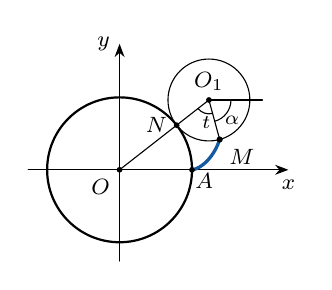
\begin{tikzpicture}[scale=0.80, >=Stealth, line cap=round, line join=round]
    % R = 1.15, r = 0.65, angle(AON) = 38 deg => t = (R/r)*38 = 67.23 deg
    \def\R{1.15}
    \def\r{0.65}
    \def\angAON{38}
    \pgfmathsetmacro{\tdeg}{\R/\r*\angAON}
    \pgfmathsetmacro{\alp}{\angAON - 180 + \tdeg}
    \coordinate (O) at (0,0);
    \coordinate (A) at (\R, 0);
    \coordinate (N) at ({\R*cos(\angAON)}, {\R*sin(\angAON)});
    \coordinate (O1) at ({(\R+\r)*cos(\angAON)}, {(\R+\r)*sin(\angAON)});
    \coordinate (M) at ({(\R+\r)*cos(\angAON) + \r*cos(\alp)}, {(\R+\r)*sin(\angAON) + \r*sin(\alp)});

    \draw[->] (-1.45, 0) -- (2.68, 0) node[below, font=\footnotesize] {$x$};
    \draw[->] (0, -1.45) -- (0, 2.00) node[left, font=\footnotesize] {$y$};

    \draw[thick] (O) circle (\R);
    \draw (O1) circle (\r);

    % 外摆线弧 AM
    \draw[very thick, curveblue, domain=0:\tdeg, samples=80, variable=\s]
      plot ({(\R+\r)*cos(\r/\R*\s) - \r*cos(\s + \r/\R*\s)},
            {(\R+\r)*sin(\r/\R*\s) - \r*sin(\s + \r/\R*\s)});

    \draw (O) -- (O1);
    \draw (O1) -- (M);
    \draw[thin] (O1) -- ++(0.85, 0);

    % 角 t (从 O1N 逆时针到 O1M)
    \draw ($(O1) + ({\angAON-180}:0.22)$) arc ({\angAON-180}:\alp:0.22);
    \node[font=\scriptsize] at ($(O1) + ({0.5*(\angAON-180+\alp)+12}:0.36)$) {$t$};

    % 角 alpha (从水平右射线顺时针到 O1M)
    \draw ($(O1) + (0:0.35)$) arc (0:\alp:0.35);
    \node[font=\scriptsize] at ($(O1) + ({0.5*\alp-4}:0.49)$) {$\alpha$};

    \fill (O) circle (1.3pt) node[below left, font=\footnotesize] {$O$};
    \fill (A) circle (1.3pt) node[below right=0.5pt, fill=white, inner sep=0.5pt, font=\footnotesize] {$A$};
    \fill (N) circle (1.3pt) node[left, font=\footnotesize] {$N$};
    \fill (O1) circle (1.3pt) node[above, font=\footnotesize] {$O_1$};
    \fill (M) circle (1.4pt) node[below right, font=\footnotesize] {$M$};
  \end{tikzpicture}
  \captionof*{figure}{图\ 27.1}
\end{minipage}
\begin{align*}
  (x, y) &= \bigl((R+r)\cos\angle AON,\, (R+r)\sin\angle AON\bigr) \\
         &\quad + (r\cos\alpha,\, r\sin\alpha) \\
         &= \biggl((R+r)\cos\frac{r}{R}t - r\cos\Bigl(t + \frac{r}{R}t\Bigr), \\
         &\qquad\ (R+r)\sin\frac{r}{R}t - r\sin\Bigl(t + \frac{r}{R}t\Bigr)\biggr).
\end{align*}
令 $\frac{r}{R}=m$，就得到外摆线的参数方程是
\begin{align*}
  x &= (R+mR)\cos mt - mR\cos(t+mt), \\
  y &= (R+mR)\sin mt - mR\sin(t+mt),
\end{align*}
其中 $m$ 可取任意正数。当 $m$ 取不同数值时，得到不同形状的外摆线。图 27.2 画出其中 $m=2$ 和 $m=\frac{3}{5}$ 的两种情形。$m=\frac{3}{5}$ 时的外摆线构成一幅美丽的图案。

\begin{figure}[htbp]
  \centering
  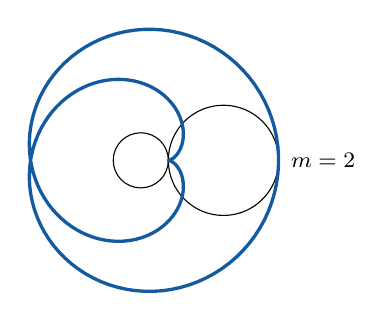
\begin{tikzpicture}[scale=0.35, line cap=round, line join=round]
    % m = 2, R = 1
    \draw (0,0) circle (1);
    \draw (3,0) circle (2);
    \draw[very thick, curveblue, domain=0:360, samples=220, variable=\t]
      plot ({3*cos(2*\t) - 2*cos(3*\t)},
            {3*sin(2*\t) - 2*sin(3*\t)});
    \node[right, font=\footnotesize] at (5.1, 0) {$m=2$};
  \end{tikzpicture}
  \hspace{6mm}
  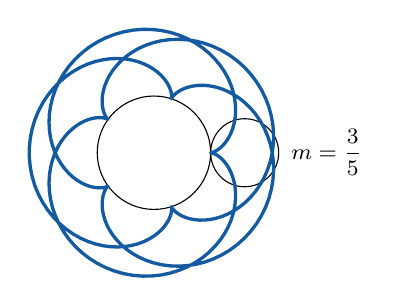
\begin{tikzpicture}[scale=0.72, line cap=round, line join=round]
    % m = 3/5, R = 1
    \draw (0,0) circle (1);
    \draw (1.6,0) circle (0.6);
    \draw[very thick, curveblue, domain=0:1800, samples=360, variable=\t]
      plot ({1.6*cos(0.6*\t) - 0.6*cos(1.6*\t)},
            {1.6*sin(0.6*\t) - 0.6*sin(1.6*\t)});
    \node[right, font=\footnotesize] at (2.25, 0) {$m=\dfrac{3}{5}$};
  \end{tikzpicture}
  \caption*{图\ 27.2}
\end{figure}

\section{曲线之心}
\markboth{28. 曲线之心}{28. 曲线之心}

当动圆半径与定圆半径相等时，外摆线的形状像一颗心脏（图 28.1），叫做心脏线。心脏线的发现者是荷兰数学家考尔斯玛（十七世纪末），命名者是意大利学者卡斯提龙（十八世纪）。

用手指按住一枚分币不动，并使另一枚同样大小的分币绕着它滚动，第二枚分币边缘上的每一点都画出一条心脏线。

在第 27 节导出的外摆线的参数方程中令 $R=r$，$m=1$，就得到心脏线的参数方程：
\[
  x = 2r\cos t - r\cos 2t,\quad y = 2r\sin t - r\sin 2t.
\]

心脏线的方程可以化成很简单的形式。为此，首先平移坐标轴，把坐标原点移到点 $A(r, 0)$。因而曲线上任意点 $M(x, y)$ 在新坐标系中的坐标成为 $(X, Y)$，这里
\begin{align*}
  X &= x - r = 2r\cos t - r\cos 2t - r \\
    &= 2r\cos t - 2r\cos^2 t \\
    &= 2r\cos t\,(1-\cos t), \\
  Y &= y = 2r\sin t - r\sin 2t \\
    &= 2r\sin t - 2r\sin t\cos t \\
    &= 2r\sin t\,(1-\cos t).
\end{align*}
由此得到
\begin{gather*}
  \frac{Y}{X} = \tg t, \\
  X^2 + Y^2 = 4r^2(1-\cos t)^2.
\end{gather*}
再化到极坐标 $(\rho, \theta)$，由于
\[
  \tg\theta = \frac{Y}{X},\quad \rho = \sqrt{X^2+Y^2},
\]
就得到心脏线的极坐标方程是
\[
  \rho = 2r(1-\cos\theta).
\]
这时极坐标系的极点是图 28.1 中的尖点 $A$，极轴是图中的射线 $Ax$。

有时也把极轴旋转 $180^\circ$，即极点还是 $A$，极轴改为射线 $AO$。这时要把 $\theta$ 换成 $\pi+\theta$，因而 $\cos\theta$ 换成 $-\cos\theta$，心脏线的极坐标方程变成
\[
  \rho = 2r(1+\cos\theta).
\]

\begin{figure}[htbp]
  \centering
  \begin{minipage}[b]{0.47\textwidth}
    \centering
    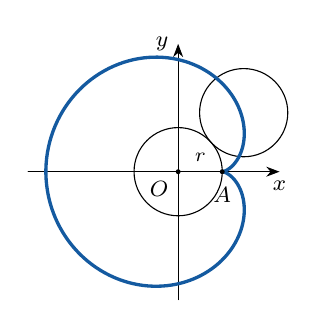
\begin{tikzpicture}[scale=0.56, >=Stealth, line cap=round, line join=round]
      \def\r{1.0}
      \def\ang{42}
      \draw[->] (-3.4, 0) -- (2.3, 0) node[below, font=\footnotesize] {$x$};
      \draw[->] (0, -2.9) -- (0, 2.9) node[left, font=\footnotesize] {$y$};

      \draw (0,0) circle (\r);
      \draw ({2*\r*cos(\ang)}, {2*\r*sin(\ang)}) circle (\r);

      \draw[very thick, curveblue, domain=0:360, samples=200, variable=\t]
        plot ({2*\r*cos(\t) - \r*cos(2*\t)},
              {2*\r*sin(\t) - \r*sin(2*\t)});

      \fill (0,0) circle (1.6pt) node[below left, font=\footnotesize] {$O$};
      \fill (\r, 0) circle (1.6pt) node[below=2pt, font=\footnotesize] {$A$};
      \node[above, font=\scriptsize] at (0.5*\r, 0) {$r$};
    \end{tikzpicture}
    \caption*{图\ 28.1}
  \end{minipage}
  \hfill
  \begin{minipage}[b]{0.47\textwidth}
    \centering
    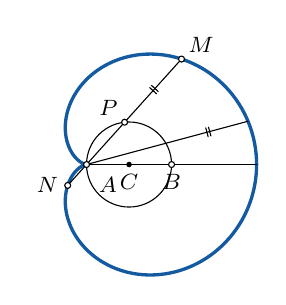
\begin{tikzpicture}[scale=0.72, >=Stealth, line cap=round, line join=round]
      \def\r{0.75}
      \def\th{48}
      \def\thb{15}
      \coordinate (A) at (0,0);
      \coordinate (C) at (\r, 0);
      \coordinate (B) at (2*\r, 0);
      \coordinate (P) at ({2*\r*cos(\th)*cos(\th)}, {2*\r*cos(\th)*sin(\th)});
      \coordinate (M) at ({2*\r*(1+cos(\th))*cos(\th)}, {2*\r*(1+cos(\th))*sin(\th)});
      \coordinate (N) at ({2*\r*(1-cos(\th))*cos(\th+180)}, {2*\r*(1-cos(\th))*sin(\th+180)});
      \coordinate (P2) at ({2*\r*cos(\thb)*cos(\thb)}, {2*\r*cos(\thb)*sin(\thb)});
      \coordinate (M2) at ({2*\r*(1+cos(\thb))*cos(\thb)}, {2*\r*(1+cos(\thb))*sin(\thb)});

      % 心脏线 rho = 2r(1 + cos theta)
      \draw[very thick, curveblue, domain=0:360, samples=200, variable=\t]
        plot ({2*\r*(1+cos(\t))*cos(\t)}, {2*\r*(1+cos(\t))*sin(\t)});

      % 圆 C 与直径射线
      \draw (C) circle (\r);
      \draw (A) -- ({4*\r}, 0);
      \draw (N) -- (M);
      \draw (A) -- (M2);

      % 等长双短线记号 (PM 与 P2M2 与直径)
      \coordinate (midPM) at ($(P)!0.5!(M)$);
      \draw ($(midPM)+(\th+90:0.08)$) -- ($(midPM)+(\th-90:0.08)$);
      \draw ($(midPM)+(\th:0.05)+(\th+90:0.08)$) -- ($(midPM)+(\th:0.05)+(\th-90:0.08)$);

      \coordinate (midPMb) at ($(P2)!0.5!(M2)$);
      \draw ($(midPMb)+(\thb+90:0.08)$) -- ($(midPMb)+(\thb-90:0.08)$);
      \draw ($(midPMb)+(\thb:0.05)+(\thb+90:0.08)$) -- ($(midPMb)+(\thb:0.05)+(\thb-90:0.08)$);

      \fill[white] (A) circle (1.5pt); \draw (A) circle (1.5pt) node[below right=1pt, font=\footnotesize] {$A$};
      \fill (C) circle (1.4pt) node[below, font=\footnotesize] {$C$};
      \fill[white] (B) circle (1.5pt); \draw (B) circle (1.5pt) node[below, font=\footnotesize] {$B$};
      \fill[white] (P) circle (1.5pt); \draw (P) circle (1.5pt) node[above left=-1pt, font=\footnotesize] {$P$};
      \fill[white] (M) circle (1.5pt); \draw (M) circle (1.5pt) node[above right=-1pt, font=\footnotesize] {$M$};
      \fill[white] (N) circle (1.5pt); \draw (N) circle (1.5pt) node[left, font=\footnotesize] {$N$};
    \end{tikzpicture}
    \caption*{图\ 28.2}
  \end{minipage}
\end{figure}

从极坐标方程可得到心脏线的一种简便画法。如图 28.2，作圆 $C$，使它的半径为 $r$。在圆周上取一个定点 $A$。过 $A$ 任意作直线，交圆 $C$ 于点 $P$。在直线 $AP$ 上向 $P$ 点两侧取 $PM=PN=AB$，这里 $AB$ 是圆 $C$ 的直径，则 $M$ 和 $N$ 是心脏线上的两个点。继续这样作出若干个点，便可根据它们描出心脏线来。

\section{利用三角板画心脏线}
\markboth{29. 利用三角板画心脏线}{29. 利用三角板画心脏线}

只要先画一个辅助圆，就能利用三角板画出一条心脏线来。

\noindent
\begin{minipage}[c]{0.42\textwidth}
  \centering
  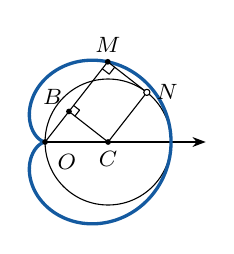
\begin{tikzpicture}[scale=0.80, >=Stealth, line cap=round, line join=round]
    % 圆 C 半径 2r = 1.0, O=(0,0), C=(1.0, 0), theta = 52 deg
    \def\rr{1.0}
    \def\th{52}
    \coordinate (O) at (0,0);
    \coordinate (C) at (\rr, 0);
    \coordinate (B) at ({\rr*cos(\th)*cos(\th)}, {\rr*cos(\th)*sin(\th)});
    \coordinate (M) at ({\rr*(1+cos(\th))*cos(\th)}, {\rr*(1+cos(\th))*sin(\th)});
    \coordinate (N) at ({\rr*(1+cos(\th))}, {\rr*sin(\th)});

    % 极轴
    \draw[->] (O) -- (2.55, 0);

    % 辅助圆 C 与心脏线
    \draw (C) circle (\rr);
    \draw[very thick, curveblue, domain=0:360, samples=200, variable=\t]
      plot ({\rr*(1+cos(\t))*cos(\t)}, {\rr*(1+cos(\t))*sin(\t)});

    % 矩形 CBMN 与线段 OM
    \draw (O) -- (M);
    \draw (C) -- (B);
    \draw (M) -- (N);
    \draw (C) -- (N);

    % 直角记号 (直角顶点 M 与垂足 B)
    \draw ($(M)+({\th-180}:0.14)$) -- ($(M)+({\th-180}:0.14)+({\th-90}:0.14)$) -- ($(M)+({\th-90}:0.14)$);
    \draw ($(B)+(\th:0.12)$) -- ($(B)+(\th:0.12)+({\th-90}:0.12)$) -- ($(B)+({\th-90}:0.12)$);

    % 关键点与标签
    \fill (O) circle (1.3pt) node[below right=1pt, font=\footnotesize] {$O$};
    \fill (C) circle (1.3pt) node[below, font=\footnotesize] {$C$};
    \fill (B) circle (1.3pt) node[above left=-1pt, font=\footnotesize] {$B$};
    \fill (M) circle (1.3pt) node[above, font=\footnotesize] {$M$};
    \fill[white] (N) circle (1.4pt); \draw (N) circle (1.4pt) node[right, font=\footnotesize] {$N$};
  \end{tikzpicture}
  \captionof*{figure}{图\ 29.1}
\end{minipage}
\hfill
\begin{minipage}[c]{0.55\textwidth}
  \setlength{\parindent}{2em}\indent
  如图 29.1，设辅助圆为圆 $C$。在圆周上任取一点 $O$。让三角板的一条直角边通过 $O$ 点，另一条直角边与圆 $C$ 相切，这时三角板的直角顶点 $M$ 就是心脏线的一个点。继续这样作出心脏线上的若干个点，最后只要用光滑曲线把这些点连起来就行了（但 $O$ 点处有一个尖角）。
\end{minipage}

为了证明上述画法的正确性，我们取 $O$ 为极点，$OC$ 为极轴，并设圆 $C$ 的半径为 $2r$。设三角板的一条直角边沿 $MN$ 与圆 $C$ 相切，切点是 $N$。作 $CB\perp OM$，垂足为 $B$（图 29.1），则 $CBMN$ 是矩形。因而
\begin{align*}
  \rho = OM &= OB + BM \\
            &= OC\cos\theta + CN \\
            &= 2r\cos\theta + 2r,
\end{align*}
即
\[
  \rho = 2r(1+\cos\theta),
\]
这正是心脏线的极坐标方程（见第 28 节）。

利用第 10 节中介绍的垂足曲线概念，上面所证明的事实可以叙述成：心脏线是一个圆关于圆周上一点的垂足曲线。

\section{帕斯卡的蜗牛}
\markboth{30. 帕斯卡的蜗牛}{30. 帕斯卡的蜗牛}

在用英语写就的数学书里，有一种曲线被叫做 Pascal's limaçon，但是这里的 limaçon 却不是一个英语单词，而是一个法语单词，意思是“蜗牛”。蜗牛是法国人爱吃的一种佳肴，这里是指曲线的形状像蜗牛。这里的 Pascal 不是十七世纪著名的法国数学家和物理学家布来兹·帕斯卡，而是他的父亲爱田·帕斯卡。如果从字面上直译，这种曲线的名称就成为“帕斯卡的蜗牛”，不过作为数学术语，却要把它译成帕斯卡蜗线，简称蜗线；也有很多人把它译成“蚶线”。这种曲线的极坐标方程可以写成
\[
  \rho = 2r\cos\theta + l,
\]
其中 $r$ 和 $l$ 是两个正数。当 $l=2r$ 时，上述方程就成为 $\rho = 2r(1+\cos\theta)$，这是心脏线的方程（见第 28 节），所以心脏线是蜗线的特例。

蜗线可以用下面的几何方式来定义：已知半径为 $r$ 的定圆，$O$ 是这个圆上的一个定点。过 $O$ 点任意作直线交这圆于第二点 $N$，在直线 $ON$ 上向 $N$ 点两侧截取 $NM = NM_1 = l$，其中 $l$ 为定长，则点 $M$ 和 $M_1$ 的轨迹叫做帕斯卡蜗线。

\begin{figure}[htbp]
  \centering
  \begin{minipage}[b]{0.32\textwidth}
    \centering
    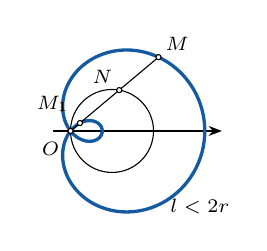
\begin{tikzpicture}[scale=0.62, >=Stealth, line cap=round, line join=round]
      \def\r{0.85}
      \def\l{1.05}
      \def\th{40}
      \coordinate (O) at (0,0);
      \coordinate (N) at ({2*\r*cos(\th)*cos(\th)}, {2*\r*cos(\th)*sin(\th)});
      \coordinate (M) at ({(2*\r*cos(\th)+\l)*cos(\th)}, {(2*\r*cos(\th)+\l)*sin(\th)});
      \coordinate (M1) at ({(2*\r*cos(\th)-\l)*cos(\th)}, {(2*\r*cos(\th)-\l)*sin(\th)});

      \draw[->] (-0.35, 0) -- (3.1, 0);
      \draw (\r, 0) circle (\r);
      \draw[very thick, curveblue, domain=0:360, samples=220, variable=\t]
        plot ({(2*\r*cos(\t)+\l)*cos(\t)}, {(2*\r*cos(\t)+\l)*sin(\t)});
      \draw (O) -- (M);

      \fill[white] (O) circle (1.5pt); \draw (O) circle (1.5pt) node[below left=0.5pt, font=\scriptsize] {$O$};
      \fill[white] (N) circle (1.5pt); \draw (N) circle (1.5pt) node[above left=-1pt, font=\scriptsize] {$N$};
      \fill[white] (M) circle (1.5pt); \draw (M) circle (1.5pt) node[above right=-1pt, font=\scriptsize] {$M$};
      \fill[white] (M1) circle (1.5pt); \draw (M1) circle (1.5pt) node[above left=0.5pt, font=\scriptsize] {$M_1$};
      \node[font=\scriptsize] at (2.65, -1.55) {$l<2r$};
    \end{tikzpicture}
    \caption*{图\ 30.1}
  \end{minipage}
  \hfill
  \begin{minipage}[b]{0.32\textwidth}
    \centering
    \begin{tikzpicture}[scale=0.55, >=Stealth, line cap=round, line join=round]
      \def\r{0.72}
      \def\l{1.44}
      \def\th{42}
      \coordinate (O) at (0,0);
      \coordinate (N) at ({2*\r*cos(\th)*cos(\th)}, {2*\r*cos(\th)*sin(\th)});
      \coordinate (M) at ({(2*\r*cos(\th)+\l)*cos(\th)}, {(2*\r*cos(\th)+\l)*sin(\th)});
      \coordinate (M1) at ({(2*\r*cos(\th)-\l)*cos(\th)}, {(2*\r*cos(\th)-\l)*sin(\th)});

      \draw[->] (-0.75, 0) -- (3.25, 0);
      \draw (\r, 0) circle (\r);
      \draw[very thick, curveblue, domain=0:360, samples=220, variable=\t]
        plot ({(2*\r*cos(\t)+\l)*cos(\t)}, {(2*\r*cos(\t)+\l)*sin(\t)});
      \draw (M1) -- (M);

      \fill[white] (O) circle (1.6pt); \draw (O) circle (1.6pt) node[below right=-1pt, font=\scriptsize] {$O$};
      \fill[white] (N) circle (1.6pt); \draw (N) circle (1.6pt) node[above left=-1pt, font=\scriptsize] {$N$};
      \fill[white] (M) circle (1.6pt); \draw (M) circle (1.6pt) node[above right=-1pt, font=\scriptsize] {$M$};
      \fill[white] (M1) circle (1.6pt); \draw (M1) circle (1.6pt) node[left, font=\scriptsize] {$M_1$};
      \node[font=\scriptsize] at (2.75, -1.65) {$l=2r$};
    \end{tikzpicture}
    \caption*{图\ 30.2}
  \end{minipage}
  \hfill
  \begin{minipage}[b]{0.32\textwidth}
    \centering
    \begin{tikzpicture}[scale=0.52, >=Stealth, line cap=round, line join=round]
      \def\r{0.62}
      \def\l{1.75}
      \def\th{42}
      \coordinate (O) at (0,0);
      \coordinate (N) at ({2*\r*cos(\th)*cos(\th)}, {2*\r*cos(\th)*sin(\th)});
      \coordinate (M) at ({(2*\r*cos(\th)+\l)*cos(\th)}, {(2*\r*cos(\th)+\l)*sin(\th)});
      \coordinate (M1) at ({(2*\r*cos(\th)-\l)*cos(\th)}, {(2*\r*cos(\th)-\l)*sin(\th)});

      \draw[->] (-1.15, 0) -- (3.35, 0);
      \draw (\r, 0) circle (\r);
      \draw[very thick, curveblue, domain=0:360, samples=220, variable=\t]
        plot ({(2*\r*cos(\t)+\l)*cos(\t)}, {(2*\r*cos(\t)+\l)*sin(\t)});
      \draw (M1) -- (M);

      \fill[white] (O) circle (1.6pt); \draw (O) circle (1.6pt) node[below right=-1pt, font=\scriptsize] {$O$};
      \fill[white] (N) circle (1.6pt); \draw (N) circle (1.6pt) node[above left=-1pt, font=\scriptsize] {$N$};
      \fill[white] (M) circle (1.6pt); \draw (M) circle (1.6pt) node[above right=-1pt, font=\scriptsize] {$M$};
      \fill[white] (M1) circle (1.6pt); \draw (M1) circle (1.6pt) node[left, font=\scriptsize] {$M_1$};
      \node[font=\scriptsize] at (2.85, -1.75) {$l>2r$};
    \end{tikzpicture}
    \caption*{图\ 30.3}
  \end{minipage}
\end{figure}

当 $l<2r$ 时，曲线的形状如图 30.1，带有一个绕扣。当 $l=2r$ 时，曲线化为心脏线（图 30.2），带有一个尖点。当 $l>2r$ 时，曲线的形状如图 30.3，既没有绕扣，也没有尖点。

\noindent
\begin{minipage}[c]{0.40\textwidth}
  \centering
  \begin{tikzpicture}[scale=0.68, >=Stealth, line cap=round, line join=round]
    % 凸轮轮廓：蜗线 rho = 2r*cos(theta - theta0) + l (2r < l < 4r 明显呈现凹弧特征)
    \def\twoR{0.84}
    \def\Lcam{1.22}
    \def\thzero{120}
    \pgfmathsetmacro{\rhoM}{\twoR*cos(90-\thzero) + \Lcam}

    % 凸轮轮廓曲线
    \draw[very thick, curveblue, domain=0:360, samples=220, variable=\t]
      plot ({(\twoR*cos(\t-\thzero)+\Lcam)*cos(\t)},
            {(\twoR*cos(\t-\thzero)+\Lcam)*sin(\t)});

    % 转轴中心与圆环
    \fill (0,0) circle (2.2pt);
    \draw (0,0) circle (0.16);

    % 极轴射线 S
    \draw (0,0) -- ({\thzero}:{\twoR+\Lcam});
    \node[left, font=\footnotesize] at ({\thzero}:{0.76*(\twoR+\Lcam)}) {$S$};

    % 竖直尖顶从动杆与导向套（尖端正抵 M 点）
    \draw[densely dashed] (0,0) -- (0, \rhoM);
    \fill (0, \rhoM) circle (1.3pt);
    \draw[thick, fill=white] (0, \rhoM) -- (-0.06, \rhoM+0.14) -- (-0.06, \rhoM+1.05) -- (0.06, \rhoM+1.05) -- (0.06, \rhoM+0.14) -- cycle;
    \draw[thick] (-0.32, \rhoM+0.44) -- (-0.06, \rhoM+0.44);
    \draw[thick] (0.06, \rhoM+0.44) -- (0.32, \rhoM+0.44);
    \draw[thick] (-0.32, \rhoM+0.80) -- (-0.06, \rhoM+0.80);
    \draw[thick] (0.06, \rhoM+0.80) -- (0.32, \rhoM+0.80);
    \node[right, font=\footnotesize] at (0.08, \rhoM+0.10) {$M$};

    % 角度 omega t
    \draw (0, 0.72) arc (90:\thzero:0.72);
    \node[font=\scriptsize, fill=white, inner sep=0.4pt] at (105:1.05) {$\omega t$};

    % 凸轮逆时针旋转指示弧箭头（不穿刺凸轮实体）
    \draw[->, thin] (-22:0.46) arc (-22:55:0.46);
  \end{tikzpicture}
  \captionof*{figure}{图\ 30.4}
\end{minipage}
\hfill
\begin{minipage}[c]{0.57\textwidth}
  \setlength{\parindent}{2em}\indent
  机器上的凸轮机构有时采用蜗线作为凸轮的轮廓曲线（图 30.4）。采用这样的凸轮轮廓曲线，当凸轮以角速度 $\omega$ 匀速旋转时，有
  \[
    \rho = 2r\cos\omega t + l,
  \]
  因而带动图中上部的从动杆沿着它所在的直线按余弦规律往返运动。在第 23 节中已经证明过，按余弦规律的往返直线运动可以减小撞击力。
\end{minipage}


% --- 批次 4：第 31–40 节 ---
\section{利用三角板画蜗线}
\markboth{31. 利用三角板画蜗线}{31. 利用三角板画蜗线}

\noindent
\begin{minipage}[t]{0.53\textwidth}
  \vspace{0pt}
  \hspace{2em}如图 31.1，先作一个半径为 $l$ 的辅助圆，设圆心为 $A$。再在平面内取一点 $O$，设 $OA=2r$。让三角板的一条直角边与圆 $A$ 相切（切点为 $D$），另一条直角边通过 $O$ 点，则三角板的直角顶点 $M$ 就是蜗线 $\rho=2r\cos\theta+l$ 上的一个点。继续这样求出若干点后，就可根据它们描出蜗线来了。
\end{minipage}
\hfill
\begin{minipage}[t]{0.44\textwidth}
  \vspace{0pt}
  \centering
  \begin{tikzpicture}[scale=0.80, >=Stealth, line cap=round, line join=round]
    % 2r = 1.38, l = 0.82, theta = 32 deg
    \def\twoR{1.38}
    \def\l{0.82}
    \def\th{32}
    \coordinate (O) at (0,0);
    \coordinate (A) at (\twoR, 0);
    \coordinate (N) at ({\twoR*cos(\th)*cos(\th)}, {\twoR*cos(\th)*sin(\th)});
    \coordinate (M) at ({(\twoR*cos(\th)+\l)*cos(\th)}, {(\twoR*cos(\th)+\l)*sin(\th)});
    \coordinate (M1) at ({(\twoR*cos(\th)-\l)*cos(\th)}, {(\twoR*cos(\th)-\l)*sin(\th)});
    \coordinate (D) at ({\twoR + \l*cos(\th)}, {\l*sin(\th)});
    \coordinate (D1) at ({\twoR - \l*cos(\th)}, {-\l*sin(\th)});

    % 极轴射线（从 O 点向右）
    \draw[->] (O) -- (2.72, 0);

    % 辅助圆 A (半径 l)
    \draw (A) circle (\l);

    % 帕斯卡蜗线 rho = 2r cos theta + l
    \draw[very thick, curveblue, domain=0:360, samples=220, variable=\t]
      plot ({(\twoR*cos(\t)+\l)*cos(\t)}, {(\twoR*cos(\t)+\l)*sin(\t)});

    % 辅助连线：OM, AN, D1-A-D, MD, M1D1
    \draw (O) -- (M);
    \draw (A) -- (N);
    \draw (D1) -- (D);
    \draw (M) -- (D);
    \draw (M1) -- (D1);

    % 直角记号 (AN perp OM, MD perp AD)
    \draw ($(N)!0.12!(O)$) -- ($($(N)!0.12!(O)$) + ($(N)!0.12!(A)$) - (N)$) -- ($(N)!0.12!(A)$);
    \draw ($(D)!0.12!(M)$) -- ($($(D)!0.12!(M)$) + ($(D)!0.12!(A)$) - (D)$) -- ($(D)!0.12!(A)$);

    % 关键点与标签
    \fill (O) circle (1.3pt) node[left=1pt, font=\footnotesize] {$O$};
    \fill (A) circle (1.3pt) node[below, font=\footnotesize] {$A$};
    \fill (N) circle (1.3pt) node[above left=-1pt, font=\footnotesize] {$N$};
    \fill (M) circle (1.4pt) node[above right=-1pt, font=\footnotesize] {$M$};
    \fill (M1) circle (1.4pt) node[above left=0.5pt, fill=white, inner sep=0.4pt, font=\footnotesize] {$M_1$};
    \fill (D) circle (1.3pt) node[below right=-2pt, font=\footnotesize] {$D$};
    \fill (D1) circle (1.3pt) node[below left=-2pt, font=\footnotesize] {$D_1$};
  \end{tikzpicture}
  \captionof*{figure}{图\ 31.1}
\end{minipage}

\medskip

为了证明上述作法的正确性，可作 $AN\perp OM$，垂足为 $N$。设 $\angle AOM=\theta$。若 $N$ 在 $O$ 与 $M$ 之间，则
\begin{align*}
  \rho = OM &= ON + NM = OA\cos\theta + AD \\
            &= 2r\cos\theta + l,
\end{align*}
所以 $M(\rho,\theta)$ 是蜗线 $\rho=2r\cos\theta+l$ 上的点。若 $M_1$ 在 $O$ 与 $N$ 之间（图 31.1），则把 $M_1$ 的极角看成 $\theta_1=\theta+\pi$，因而它的极半径 $\rho_1$ 是负的：
\begin{align*}
  \rho_1 = -OM_1 &= -ON + M_1N = -OA\cos\theta + D_1A \\
                 &= -2r\cos\theta + l = 2r\cos(\theta+\pi) + l \\
                 &= 2r\cos\theta_1 + l,
\end{align*}
所以 $M_1(\rho_1,\theta_1)$ 也是蜗线 $\rho=2r\cos\theta+l$ 上的点。

利用垂足曲线的概念（第 10 节），可以把上面证明的事实叙述成：定圆关于它所在平面内任一定点的垂足曲线是帕斯卡蜗线。当定点在圆外时（$2r>l$），得到有绕扣的蜗线；当定点在圆周上时（$2r=l$），得到有尖点的蜗线，即心脏线；当定点在圆内时（$2r<l$），得到无绕扣又无尖点的蜗线。当定点为圆心这一特殊情形时，$r=0$，垂足曲线仍为原来的圆 $\rho=l$。

\section{柴油机与垂足曲线}
\markboth{32. 柴油机与垂足曲线}{32. 柴油机与垂足曲线}

为了说明在柴油机中怎样巧妙地利用曲线的性质，需要简短地回顾几项已经知道的事实：第一，当机器中的某个部件需要以很快的节奏作往返直线运动时，为了在改变运动方向时减小撞击力，最好使它的位移按余弦规律变化（第 23 节）；第二，对于帕斯卡蜗线 $\rho=2r\cos\theta+l$（第 30 节），当极角 $\theta$ 随时间匀速变化时，极半径 $\rho$ 按余弦规律变化；第三，圆 $O$ 关于任意点 $F$ 的垂足曲线是帕斯卡蜗线，只有当点 $F$ 与圆心 $O$ 重合时，垂足曲线仍为圆 $O$（第 31 节）。

我们知道，柴油发动机工作情形是周而复始的，每个周期由进气、压缩、做功、排气四个步骤组成，这四步叫做四个冲程。为了保证这四个冲程能顺次衔接，循环不已，柴油机的进气阀门和排气阀门必须按一定规律周期性地定时开闭。阀门打开或关闭，是靠一根挺杆沿直线往返运动，从而顶起或放下阀门。由于柴油机转速很快，所以为了减小撞击力，挺杆沿直线往返运动时的行程最好能按余弦规律变化。在柴油机中利用如图 32.1 所示的凸轮来控制挺杆的运动。

\begin{figure}[htbp]
  \centering
  \begin{minipage}[b]{0.48\textwidth}
    \centering
    \begin{tikzpicture}[scale=1.05, line cap=round, line join=round]
      % 四段光滑圆弧凸轮几何参数
      \def\rO{0.68}
      \def\dM{1.42}
      \def\th{12}
      \def\hP{0.62}
      \pgfmathsetmacro{\Mx}{-\dM*cos(\th)}
      \pgfmathsetmacro{\My}{-\dM*sin(\th)}
      \pgfmathsetmacro{\RM}{\dM + \rO}
      \pgfmathsetmacro{\phiD}{atan2(\hP - \My, -\Mx)}
      \pgfmathsetmacro{\MP}{veclen(-\Mx, \hP - \My)}
      \pgfmathsetmacro{\RP}{\RM - \MP}

      \coordinate (O) at (0,0);
      \coordinate (B) at (0, -\rO);
      \coordinate (P) at (0, \hP);
      \coordinate (E) at (0, \hP + \RP);
      \coordinate (M) at (\Mx, \My);
      \coordinate (N) at (-\Mx, \My);
      \coordinate (C) at ({\rO*cos(\th)}, {\rO*sin(\th)});
      \coordinate (A) at ({-\rO*cos(\th)}, {\rO*sin(\th)});
      \coordinate (D) at ({\Mx + \RM*cos(\phiD)}, {\My + \RM*sin(\phiD)});
      \coordinate (F) at ({-\Mx - \RM*cos(\phiD)}, {\My + \RM*sin(\phiD)});

      % 凸轮四段圆弧轮廓
      \draw[very thick, curveblue]
        (A) arc ({180-\th}:{360+\th}:\rO)
        arc (\th:\phiD:\RM)
        arc (\phiD:{180-\phiD}:\RP)
        arc ({180-\phiD}:{180-\th}:\RM);

      % 虚线辅助射线
      \draw[densely dashed] (B) -- (E);
      \draw[densely dashed] (M) -- (C);
      \draw[densely dashed] (N) -- (A);
      \draw[densely dashed] (M) -- (D);
      \draw[densely dashed] (N) -- (F);

      % 各点标记
      \fill (O) circle (1.2pt) node[left=1pt, yshift=-3pt, font=\scriptsize] {$O$};
      \fill (P) circle (1.2pt) node[right, font=\scriptsize] {$P$};
      \fill (M) circle (1.2pt) node[below, font=\scriptsize] {$M$};
      \fill (N) circle (1.2pt) node[below, font=\scriptsize] {$N$};
      \fill (A) circle (1.1pt) node[left, font=\scriptsize] {$A$};
      \fill (B) circle (1.1pt) node[below, font=\scriptsize] {$B$};
      \fill (C) circle (1.1pt) node[right, font=\scriptsize] {$C$};
      \fill (D) circle (1.1pt) node[above right=-1pt, font=\scriptsize] {$D$};
      \fill (E) circle (1.1pt) node[above right=-1pt, font=\scriptsize] {$E$};
      \fill (F) circle (1.1pt) node[above left=-1pt, font=\scriptsize] {$F$};
    \end{tikzpicture}
    \caption*{图\ 32.1}
  \end{minipage}
  \hfill
  \begin{minipage}[b]{0.48\textwidth}
    \centering
    \begin{tikzpicture}[scale=1.05, line cap=round, line join=round]
      \def\rO{0.68}
      \def\dM{1.42}
      \def\th{12}
      \def\hP{0.62}
      \def\rot{-30}
      \pgfmathsetmacro{\Mx}{-\dM*cos(\th)}
      \pgfmathsetmacro{\My}{-\dM*sin(\th)}
      \pgfmathsetmacro{\RM}{\dM + \rO}
      \pgfmathsetmacro{\phiD}{atan2(\hP - \My, -\Mx)}
      \pgfmathsetmacro{\MP}{veclen(-\Mx, \hP - \My)}
      \pgfmathsetmacro{\RP}{\RM - \MP}
      % 旋转 rot=-30 deg 后弧 DEF 的圆心 P' 与最高接触点 X
      \pgfmathsetmacro{\Px}{-\hP*sin(\rot)}
      \pgfmathsetmacro{\Py}{\hP*cos(\rot)}
      \pgfmathsetmacro{\yTop}{\Py + \RP}

      \coordinate (O) at (0,0);
      \coordinate (Y) at (0, \yTop);
      \coordinate (X) at (\Px, \yTop);

      % 旋转后的凸轮轮廓
      \begin{scope}[rotate=\rot]
        \draw[very thick, curveblue]
          ({-\rO*cos(\th)}, {\rO*sin(\th)}) arc ({180-\th}:{360+\th}:\rO)
          arc (\th:\phiD:\RM)
          arc (\phiD:{180-\phiD}:\RP)
          arc ({180-\phiD}:{180-\th}:\RM);
      \end{scope}

      % 中心线 l 与连线 OX, OY 及直角记号
      \draw (0, -0.95) -- (0, \yTop + 1.05) node[above, font=\scriptsize] {$l$};
      \draw (O) -- (X);
      \draw[thin] (-0.95, 0) -- (0.95, 0);
      \draw (0, \yTop - 0.11) -- (0.11, \yTop - 0.11) -- (0.11, \yTop);

      % 挺杆平底与圆柱杆（带剖面斜线）
      \draw[thick] (-0.75, \yTop) -- (0.75, \yTop);
      \draw[thick] (-0.75, \yTop) -- (-0.65, \yTop + 0.14) -- (-0.18, \yTop + 0.18) -- (-0.18, \yTop + 0.85);
      \draw[thick] (0.75, \yTop) -- (0.65, \yTop + 0.14) -- (0.18, \yTop + 0.18) -- (0.18, \yTop + 0.85);
      \draw[pattern=north east lines, pattern color=mutedgray!70]
        (-0.18, \yTop + 0.45) rectangle (0.18, \yTop + 0.85);

      % 标注
      \fill (O) circle (1.2pt) node[below left=-1pt, font=\scriptsize] {$O$};
      \fill (Y) circle (1.2pt) node[left=0pt, yshift=-4pt, font=\scriptsize] {$Y$};
      \fill (X) circle (1.2pt) node[below right=-1pt, font=\scriptsize] {$X$};
      \node[right, font=\scriptsize] at (0.68, -0.25) {$c$};
    \end{tikzpicture}
    \caption*{图\ 32.2}
  \end{minipage}
\end{figure}

凸轮的轮廓由四段圆弧光滑连接而成：$\arc{ABC}$，圆心是 $O$；$\arc{CD}$，圆心是 $M$；$\arc{DEF}$，圆心是 $P$；$\arc{FA}$，圆心是 $N$。凸轮和挺杆按图 32.2 所示的方式配合：挺杆的中心线 $l$ 通过凸轮的旋转中心 $O$，挺杆的下端是垂直于 $l$ 的一个平面，设这个平面与 $l$ 的交点是 $Y$，与凸轮的接触点是 $X$，则 $XY$ 是凸轮轮廓曲线的切线，并且 $OY\perp XY$。因而当点 $X$ 沿着凸轮的轮廓曲线 $c$ 移动时，对应的点 $Y$ 就画出曲线 $c$ 关于点 $O$ 的垂足曲线。曲线 $c$ 上的圆弧 $\arc{CD}$、$\arc{DEF}$ 和 $\arc{FA}$ 的圆心都不是 $O$，所以这三部分的垂足曲线都是帕斯卡蜗线，随着凸轮绕 $O$ 点匀速旋转，挺杆沿直线 $l$ 按余弦规律作往返运动，完成开阀门和关阀门的动作。曲线 $c$ 上的圆弧 $\arc{ABC}$ 的圆心就是 $O$ 点\footnote{重排校订：原书第 51 页此处误将轮廓曲线记号小写 $c$ 印作大写 $C$，据上文“轮廓曲线 $c$”统一订正为 $c$。}，% 原书此处误印作“C”
因而这段弧关于 $O$ 点的垂足曲线还是它自己，这时点 $Y$ 与 $X$ 重合，当凸轮用这段弧与挺杆接触时，挺杆保持不动，使阀门保持关闭状态。

从上面的分析看出，为了使挺杆能迅速而平稳地完成开门和关门的动作，需要使挺杆中心线上的点 $Y$ 在凸轮平面内的轨迹是帕斯卡蜗线。由于设计者把挺杆与凸轮的接触面做成垂直于 $l$ 的平面，巧妙地利用了垂足曲线的性质，使凸轮的轮廓曲线简化为几段圆弧。制造圆弧轮廓的凸轮，比制造蜗线轮廓的凸轮容易得多了。

\section{蜗线也是外摆线}
\markboth{33. 蜗线也是外摆线}{33. 蜗线也是外摆线}

如图 33.1，设动圆 $C$ 和定圆 $O$ 的半径相等，$P$ 是在动圆平面内与动圆固定连接的一点。当圆 $C$ 在圆 $O$ 外面绕着圆 $O$ 无滑动地滚动时，$P$ 点的轨迹是一条帕斯卡蜗线，证明如下。

\begin{figure}[htbp]
  \centering
  \begin{minipage}[b]{0.47\textwidth}
    \centering
    \begin{tikzpicture}[scale=0.92, >=Stealth, line cap=round, line join=round]
      % l/2 = 0.45, l = 0.90, r = 0.68, theta = 36 deg
      \def\l{0.90}
      \def\r{0.68}
      \def\th{36}
      \coordinate (O) at (0,0);
      \coordinate (C) at ({\l*cos(\th)}, {\l*sin(\th)});
      \coordinate (P) at ({\l*cos(\th) + \r*cos(2*\th)}, {\l*sin(\th) + \r*sin(2*\th)});

      % 坐标轴
      \draw[->] (-1.15, 0) -- (1.85, 0) node[below, font=\footnotesize] {$x$};
      \draw[->] (0, -1.65) -- (0, 1.65) node[left, font=\footnotesize] {$y$};

      % 定圆 O 与动圆 C
      \draw (O) circle (0.5*\l);
      \draw (C) circle (0.5*\l);
      \draw (O) -- (C) -- (P);

      % 帕斯卡蜗线轨迹
      \draw[very thick, curveblue, domain=0:360, samples=220, variable=\t]
        plot ({\l*cos(\t) + \r*cos(2*\t)}, {\l*sin(\t) + \r*sin(2*\t)});

      \fill (O) circle (1.2pt) node[below right=-1pt, font=\footnotesize] {$O$};
      \fill (C) circle (1.2pt) node[below right=-1pt, font=\footnotesize] {$C$};
      \fill (P) circle (1.4pt) node[above right=-1pt, font=\footnotesize] {$P$};
    \end{tikzpicture}
    \caption*{图\ 33.1}
  \end{minipage}
  \hfill
  \begin{minipage}[b]{0.49\textwidth}
    \centering
    \begin{tikzpicture}[scale=0.88, >=Stealth, line cap=round, line join=round]
      % l/2 = 0.65 => l = 1.30, r = 0.85, theta = 40 deg
      \def\l{1.30}
      \def\r{0.85}
      \def\th{40}
      \pgfmathsetmacro{\Cx}{\l*cos(\th)}
      \pgfmathsetmacro{\Cy}{\l*sin(\th)}
      \pgfmathsetmacro{\Gx}{\Cx - \Cy*cos(2*\th)/sin(2*\th)}
      \coordinate (O) at (0,0);
      \coordinate (O1) at (-\r, 0);
      \coordinate (E) at (0.5*\l, 0);
      \coordinate (C0) at (\l, 0);
      \coordinate (P0) at (\l+\r, 0);
      \coordinate (D) at ({0.5*\l*cos(\th)}, {0.5*\l*sin(\th)});
      \coordinate (C) at (\Cx, \Cy);
      \coordinate (F) at ({\Cx - 0.5*\l*cos(2*\th)}, {\Cy - 0.5*\l*sin(2*\th)});
      \coordinate (G) at (\Gx, 0);
      \coordinate (P) at ({\Cx + \r*cos(2*\th)}, {\Cy + \r*sin(2*\th)});

      % 坐标轴
      \draw[->] (-1.15, 0) -- (2.45, 0) node[below, font=\footnotesize] {$x$};
      \draw[->] (0, -0.95) -- (0, 1.95) node[left, font=\footnotesize] {$y$};

      % 定圆 O、初始圆 C0（虚线）与当前动圆 C
      \draw (O) circle (0.5*\l);
      \draw[densely dashed] (C0) circle (0.5*\l);
      \draw (C) circle (0.5*\l);

      % 辅助线段
      \draw (O) -- (C) -- (P);
      \draw (O1) -- (P);
      \draw (C) -- (G);
      \draw[densely dashed] (C) -- ++(0.72, 0);

      % 角度标注
      \draw (0.34, 0) arc (0:\th:0.34);
      \node[font=\scriptsize] at ({0.5*\th}:0.49) {$\theta$};

      \draw ($(C) + ({180+\th}:0.28)$) arc ({180+\th}:{180+2*\th}:0.28);
      \node[font=\scriptsize, fill=white, inner sep=0.4pt] at ($(C) + ({180+1.5*\th}:0.47)$) {$\theta$};

      \draw ($(C) + (0:0.30)$) arc (0:{2*\th}:0.30);
      \node[font=\scriptsize] at ($(C) + (\th:0.46)$) {$\alpha$};

      % 关键点与标签
      \fill (O) circle (1.1pt) node[below left=-1pt, font=\scriptsize] {$O$};
      \fill (O1) circle (1.1pt) node[below, font=\scriptsize] {$O_1$};
      \fill (E) circle (1.1pt) node[below right=-1.5pt, fill=white, inner sep=0.3pt, font=\scriptsize] {$E$};
      \fill (G) circle (1.1pt) node[below=-1pt, font=\scriptsize] {$G$};
      \fill (C0) circle (1.1pt) node[below right=-2pt, font=\scriptsize] {$C_0$};
      \fill (P0) circle (1.1pt) node[below, font=\scriptsize] {$P_0$};
      \fill (D) circle (1.1pt) node[above left=0.5pt, fill=white, inner sep=0.3pt, font=\scriptsize] {$D$};
      \fill (C) circle (1.1pt) node[above left=-2pt, font=\scriptsize] {$C$};
      \fill (F) circle (1.1pt) node[above right=-2pt, font=\scriptsize] {$F$};
      \fill (P) circle (1.3pt) node[above, font=\scriptsize] {$P$};
    \end{tikzpicture}
    \caption*{图\ 33.2}
  \end{minipage}
\end{figure}

设圆 $O$ 和圆 $C$ 的半径为 $\frac{l}{2}$，$CP=r$。如图 33.2，$C$ 和 $P$ 的初始位置 $C_0$ 和 $P_0$ 在 $x$ 轴上，$E$ 是圆 $O$ 和圆 $C_0$ 的切点。当圆 $C$ 滚动到图 33.2 的位置时，因为圆 $C$ 和圆 $O$ 相等，$\arc{DE}=\arc{DF}$，所以可设 $\angle COE=\angle OCF=\theta$，于是 $\overrightarrow{CP}$ 的幅角 $\alpha=2\theta$，由 $\overrightarrow{OP}=\overrightarrow{OC}+\overrightarrow{CP}$ 得向量 $\overrightarrow{OP}$ 的坐标表示式为
\begin{align*}
  (x, y) &= (l\cos\theta,\, l\sin\theta) + (r\cos\alpha,\, r\sin\alpha) \\
         &= (l\cos\theta + r\cos 2\theta,\, l\sin\theta + r\sin 2\theta).
\end{align*}
在图 33.2 中，取 $OO_1=CP=r$，把坐标原点平移到 $O_1$，得到 $P$ 点的新坐标为
\begin{align*}
  X &= l\cos\theta + r\cos 2\theta + r, \\
  Y &= l\sin\theta + r\sin 2\theta.
\end{align*}
取 $O_1$ 为极点，$O_1O$ 为极轴，设 $P$ 点的极坐标为 $(\rho, \theta)$，则易证
\[
  \angle OO_1P = \theta,\quad O_1P = \rho = \sqrt{X^2+Y^2} = 2r\cos\theta + l.
\]
这就证明了 $P$ 点的轨迹是帕斯卡蜗线 $\rho=2r\cos\theta+l$。

当 $P$ 点在动圆外部时，$P$ 到圆心 $C$ 的距离 $r$ 大于圆 $C$ 的半径 $\frac{l}{2}$，即 $2r>l$，这时得到带绕扣的蜗线。当 $P$ 在动圆的圆周上时，$r=\frac{l}{2}$，即 $2r=l$，这时得到带尖点的蜗线，即心脏线。当 $P$ 在动圆内部时，$r<\frac{l}{2}$，即 $2r<l$，这时得到无绕扣又无尖点的蜗线。

\section{变幅外摆线}
\markboth{34. 变幅外摆线}{34. 变幅外摆线}

设圆 $O$ 是一个定圆，圆 $O_1$ 是与圆 $O$ 相切的动圆，$M$ 是固定在圆 $O_1$ 平面内的一点，但不在圆 $O_1$ 的圆周上。当圆 $O_1$ 在圆 $O$ 外面绕圆 $O$ 无滑动地滚动时，$M$ 的轨迹叫做变幅外摆线。

变幅外摆线可分成两类：当 $M$ 在动圆 $O_1$ 内部时，曲线叫做短幅外摆线；当 $M$ 在动圆 $O_1$ 外部时，曲线叫做长幅外摆线。

例如，当动圆与定圆相等时，根据第 33 节可知长幅外摆线成为带绕扣的帕斯卡蜗线，短幅外摆线是无绕扣又无尖点的蜗线，而外摆线则是带尖点的蜗线，即心脏线。

\noindent
\begin{minipage}[t]{0.44\textwidth}
  \vspace{0pt}
  \centering
  \begin{tikzpicture}[scale=0.80, >=Stealth, line cap=round, line join=round]
    % R = 1.15, r = 0.55, h = 0.34, angle(AON) = 45 deg
    \def\R{1.15}
    \def\r{0.55}
    \def\h{0.34}
    \def\angAON{45}
    \pgfmathsetmacro{\tdeg}{\R/\r*\angAON}
    \pgfmathsetmacro{\alp}{\angAON - 180 + \tdeg}
    \coordinate (O) at (0,0);
    \coordinate (O1) at ({(\R+\r)*cos(\angAON)}, {(\R+\r)*sin(\angAON)});
    \coordinate (M) at ({(\R+\r)*cos(\angAON) + \h*cos(\alp)}, {(\R+\r)*sin(\angAON) + \h*sin(\alp)});

    \draw[->] (-1.35, 0) -- (2.45, 0) node[below, font=\footnotesize] {$x$};
    \draw[->] (0, -1.35) -- (0, 2.05) node[left, font=\footnotesize] {$y$};

    % 定圆 O，当前动圆 O1，初始动圆（虚线）
    \draw[thick] (O) circle (\R);
    \draw (O1) circle (\r);
    \draw[densely dashed] (\R+\r, 0) circle (\r);
    \fill (\R+\r, 0) circle (1.2pt);
    \fill (\R+\r-\h, 0) circle (1.2pt);

    % 连线与半径标示
    \draw (O) -- (O1) node[midway, above left=-2pt, font=\scriptsize] {$R$};
    \draw (O1) -- (M);
    \draw[thin] (O1) -- ++(0.65, 0);
    \draw (O1) -- ($(O1) + (75:\r)$) node[midway, left=-1pt, font=\scriptsize] {$r$};

    % 角 t 与 角 alpha
    \draw ($(O1) + ({\angAON-180}:0.18)$) arc ({\angAON-180}:\alp:0.18);
    \node[font=\scriptsize] at ($(O1) + ({0.5*(\angAON-180+\alp)}:0.29)$) {$t$};
    \draw ($(O1) + (0:0.28)$) arc (0:\alp:0.28);
    \node[font=\scriptsize] at ($(O1) + ({0.5*\alp}:0.42)$) {$\alpha$};

    \fill (O) circle (1.3pt) node[below left, font=\footnotesize] {$O$};
    \fill (O1) circle (1.3pt) node[above left=-2pt, font=\footnotesize] {$O_1$};
    \fill (M) circle (1.4pt) node[below=-1pt, font=\footnotesize] {$M$};
  \end{tikzpicture}
  \captionof*{figure}{图\ 34.1}
\end{minipage}
\hfill
\begin{minipage}[t]{0.53\textwidth}
  \vspace{0pt}
  \hspace{2em}如图 34.1，设定圆 $O$ 的半径为 $R$，动圆 $O_1$ 的半径为 $r$，点 $M$ 到 $O_1$ 的距离为 $h$。取 $O$ 为坐标原点，并且选取 $x$ 轴，使当 $O_1$ 转动到 $x$ 轴正半轴上时，射线 $O_1M$ 与 $O_1O$ 同向。又设当圆 $O_1$ 滚动到图 34.1 中的任意位置时，点 $M$ 的坐标为 $(x, y)$，$\angle OO_1M = t$。仿照 27 节外摆线的求法，知 $\overrightarrow{O_1M}$ 的幅角 $\alpha = \frac{r}{R}t - \pi + t$。因为 $\overrightarrow{OM} = \overrightarrow{OO_1} + \overrightarrow{O_1M}$，所以向量 $\overrightarrow{OM}$ 的坐标表示式为
\end{minipage}

\begin{align*}
  (x, y) &= \Bigl((R+r)\cos\frac{r}{R}t,\, (R+r)\sin\frac{r}{R}t\Bigr) + (h\cos\alpha,\, h\sin\alpha) \\
         &= \biggl((R+r)\cos\frac{r}{R}t - h\cos\Bigl(t + \frac{r}{R}t\Bigr), \\
         &\qquad\ (R+r)\sin\frac{r}{R}t - h\sin\Bigl(t + \frac{r}{R}t\Bigr)\biggr).
\end{align*}
令 $\frac{r}{R}=m$，就得到曲线的参数方程为
\[
  \begin{aligned}
    x &= (R+mR)\cos mt - h\cos(t+mt), \\
    y &= (R+mR)\sin mt - h\sin(t+mt).
  \end{aligned}
  \quad (m>0)
\]
当 $h>mR$ 时曲线为长幅外摆线，$h<mR$ 时为短幅外摆线。若 $h=mR$，则上述方程化为外摆线的方程。

在图 34.2～34.4 中分别画出了 $m=\frac{1}{4}$ 时的长幅外摆线、外摆线和短幅外摆线。

\begin{figure}[htbp]
  \centering
  \begin{minipage}[b]{0.32\textwidth}
    \centering
    \begin{tikzpicture}[scale=0.72, line cap=round, line join=round]
      % m = 1/4, R = 1, r = 0.25, h = 0.42 (长幅外摆线)
      \def\R{1.0}
      \def\r{0.25}
      \def\h{0.42}
      \def\ang{28}
      \pgfmathsetmacro{\tdeg}{\R/\r*\ang}
      \pgfmathsetmacro{\alp}{\ang - 180 + \tdeg}
      \draw (0,0) circle (\R);
      \draw ({(\R+\r)*cos(\ang)}, {(\R+\r)*sin(\ang)}) circle (\r);
      \draw ({(\R+\r)*cos(\ang)}, {(\R+\r)*sin(\ang)}) -- ({(\R+\r)*cos(\ang)+\h*cos(\alp)}, {(\R+\r)*sin(\ang)+\h*sin(\alp)});
      \fill ({(\R+\r)*cos(\ang)}, {(\R+\r)*sin(\ang)}) circle (0.9pt);
      \fill ({(\R+\r)*cos(\ang)+\h*cos(\alp)}, {(\R+\r)*sin(\ang)+\h*sin(\alp)}) circle (1.3pt);
      \draw[very thick, curveblue, domain=0:1440, samples=260, variable=\s]
        plot ({(\R+\r)*cos(0.25*\s) - \h*cos(1.25*\s)},
              {(\R+\r)*sin(0.25*\s) - \h*sin(1.25*\s)});
    \end{tikzpicture}
    \caption*{图\ 34.2}
  \end{minipage}
  \hfill
  \begin{minipage}[b]{0.32\textwidth}
    \centering
    \begin{tikzpicture}[scale=0.72, line cap=round, line join=round]
      % m = 1/4, R = 1, r = 0.25, h = 0.25 (外摆线)
      \def\R{1.0}
      \def\r{0.25}
      \def\h{0.25}
      \def\ang{28}
      \pgfmathsetmacro{\tdeg}{\R/\r*\ang}
      \pgfmathsetmacro{\alp}{\ang - 180 + \tdeg}
      \draw (0,0) circle (\R);
      \draw ({(\R+\r)*cos(\ang)}, {(\R+\r)*sin(\ang)}) circle (\r);
      \draw ({(\R+\r)*cos(\ang)}, {(\R+\r)*sin(\ang)}) -- ({(\R+\r)*cos(\ang)+\h*cos(\alp)}, {(\R+\r)*sin(\ang)+\h*sin(\alp)});
      \fill ({(\R+\r)*cos(\ang)}, {(\R+\r)*sin(\ang)}) circle (0.9pt);
      \fill ({(\R+\r)*cos(\ang)+\h*cos(\alp)}, {(\R+\r)*sin(\ang)+\h*sin(\alp)}) circle (1.3pt);
      \draw[very thick, curveblue, domain=0:1440, samples=260, variable=\s]
        plot ({(\R+\r)*cos(0.25*\s) - \h*cos(1.25*\s)},
              {(\R+\r)*sin(0.25*\s) - \h*sin(1.25*\s)});
    \end{tikzpicture}
    \caption*{图\ 34.3}
  \end{minipage}
  \hfill
  \begin{minipage}[b]{0.32\textwidth}
    \centering
    \begin{tikzpicture}[scale=0.72, line cap=round, line join=round]
      % m = 1/4, R = 1, r = 0.25, h = 0.14 (短幅外摆线)
      \def\R{1.0}
      \def\r{0.25}
      \def\h{0.14}
      \def\ang{28}
      \pgfmathsetmacro{\tdeg}{\R/\r*\ang}
      \pgfmathsetmacro{\alp}{\ang - 180 + \tdeg}
      \draw (0,0) circle (\R);
      \draw ({(\R+\r)*cos(\ang)}, {(\R+\r)*sin(\ang)}) circle (\r);
      \draw ({(\R+\r)*cos(\ang)}, {(\R+\r)*sin(\ang)}) -- ({(\R+\r)*cos(\ang)+\h*cos(\alp)}, {(\R+\r)*sin(\ang)+\h*sin(\alp)});
      \fill ({(\R+\r)*cos(\ang)}, {(\R+\r)*sin(\ang)}) circle (0.9pt);
      \fill ({(\R+\r)*cos(\ang)+\h*cos(\alp)}, {(\R+\r)*sin(\ang)+\h*sin(\alp)}) circle (1.3pt);
      \draw[very thick, curveblue, domain=0:1440, samples=260, variable=\s]
        plot ({(\R+\r)*cos(0.25*\s) - \h*cos(1.25*\s)},
              {(\R+\r)*sin(0.25*\s) - \h*sin(1.25*\s)});
    \end{tikzpicture}
    \caption*{图\ 34.4}
  \end{minipage}
\end{figure}

由于变幅外摆线和外摆线的方程可以写成上面的统一形式，所以有时也把它们统称为外摆线族曲线。

\noindent
\begin{minipage}[t]{0.53\textwidth}
  \vspace{0pt}
  \hspace{2em}外摆线族曲线的方程还可写成其它形式。例如，设 $W$ 是与 $M$ 关于 $O_1$ 对称的点，那么 $W$ 的轨迹与 $M$ 的轨迹形状相同，仅仅是位置不同。如图 34.5，有
  \begin{gather*}
    \angle OO_1M = t,\quad O_1W = h, \\
    \text{向量 }\overrightarrow{O_1W}\text{ 的幅角 }\beta = t + \frac{r}{R}t = t + mt,
  \end{gather*}
\end{minipage}
\hfill
\begin{minipage}[t]{0.44\textwidth}
  \vspace{0pt}
  \centering
  \begin{tikzpicture}[scale=0.80, >=Stealth, line cap=round, line join=round]
    % R = 1.15, r = 0.55, h = 0.34, angle(AON) = 45 deg
    \def\R{1.15}
    \def\r{0.55}
    \def\h{0.34}
    \def\angAON{45}
    \pgfmathsetmacro{\tdeg}{\R/\r*\angAON}
    \pgfmathsetmacro{\alp}{\angAON - 180 + \tdeg}
    \pgfmathsetmacro{\bet}{\angAON + \tdeg}
    \coordinate (O) at (0,0);
    \coordinate (O1) at ({(\R+\r)*cos(\angAON)}, {(\R+\r)*sin(\angAON)});
    \coordinate (M) at ({(\R+\r)*cos(\angAON) + \h*cos(\alp)}, {(\R+\r)*sin(\angAON) + \h*sin(\alp)});
    \coordinate (W) at ({(\R+\r)*cos(\angAON) + \h*cos(\bet)}, {(\R+\r)*sin(\angAON) + \h*sin(\bet)});

    \draw[->] (-1.30, 0) -- (2.40, 0) node[below, font=\footnotesize] {$x$};
    \draw[->] (0, -1.30) -- (0, 2.00) node[left, font=\footnotesize] {$y$};

    \draw[thick] (O) circle (\R);
    \draw (O1) circle (\r);
    \draw (O) -- (O1);
    \draw (M) -- (W);
    \draw[thin] (O1) -- ++(0.68, 0);

    % 角 t 与 角 beta
    \draw ($(O1) + ({\angAON-180}:0.20)$) arc ({\angAON-180}:\alp:0.20);
    \node[font=\scriptsize] at ($(O1) + ({0.5*(\angAON-180+\alp)}:0.32)$) {$t$};
    \draw ($(O1) + (0:0.25)$) arc (0:\bet:0.25);
    \node[font=\scriptsize] at ($(O1) + ({0.5*\bet}:0.38)$) {$\beta$};

    \fill (O) circle (1.2pt) node[below left, font=\footnotesize] {$O$};
    \fill (O1) circle (1.2pt) node[left=1pt, font=\footnotesize] {$O_1$};
    \fill (M) circle (1.2pt) node[below, font=\footnotesize] {$M$};
    \fill (W) circle (1.3pt) node[above left=-1pt, font=\footnotesize] {$W$};
  \end{tikzpicture}
  \captionof*{figure}{图\ 34.5}
\end{minipage}

\noindent
所以由 $\overrightarrow{OW}=\overrightarrow{OO_1}+\overrightarrow{O_1W}$ 可以得到点 $W$ 的坐标是
\[
  \begin{aligned}
    x &= (R+mR)\cos mt + h\cos(t+mt), \\
    y &= (R+mR)\sin mt + h\sin(t+mt).
  \end{aligned}
  \quad (m>0)
\]

\section{变幅内摆线}
\markboth{35. 变幅内摆线}{35. 变幅内摆线}

设 $r<R$，当半径为 $r$ 的动圆 $O_1$ 在半径为 $R$ 的定圆 $O$ 内无滑动地滚动时，在圆 $O_1$ 平面内与圆 $O_1$ 固定连结但不在 $O_1$ 圆周上的一点 $M$ 的轨迹叫做变幅内摆线。

变幅内摆线可分成两类：当 $M$ 在圆 $O_1$ 外部时，曲线称为长幅内摆线；而当 $M$ 在圆 $O_1$ 内部时，称为短幅内摆线。

如果 $M$ 在圆 $O_1$ 的圆周上，那么 $M$ 的轨迹成为内摆线，这在前面第 24 节中已经讨论过。内摆线和变幅内摆线统称为内摆线族曲线。

例如，在第 22 节中讨论卡丹的转盘问题时，我们实际上已经证明了，当动圆半径等于定圆半径的一半时，长幅内摆线和短幅内摆线都是椭圆。

\noindent
\begin{minipage}[t]{0.44\textwidth}
  \vspace{0pt}
  \centering
  \begin{tikzpicture}[scale=0.84, >=Stealth, line cap=round, line join=round]
    % R = 1.52, r = 0.66, h = 0.40, angle(AON) = 52 deg
    \def\R{1.52}
    \def\r{0.66}
    \def\h{0.40}
    \def\angAON{52}
    \pgfmathsetmacro{\tdeg}{\R/\r*\angAON}
    \pgfmathsetmacro{\alp}{\angAON - \tdeg}
    \coordinate (O) at (0,0);
    \coordinate (N) at ({\R*cos(\angAON)}, {\R*sin(\angAON)});
    \coordinate (O1) at ({(\R-\r)*cos(\angAON)}, {(\R-\r)*sin(\angAON)});
    \coordinate (M) at ({(\R-\r)*cos(\angAON) + \h*cos(\alp)}, {(\R-\r)*sin(\angAON) + \h*sin(\alp)});

    \draw[->] (-1.70, 0) -- (1.88, 0) node[below, font=\footnotesize] {$x$};
    \draw[->] (0, -1.70) -- (0, 1.88) node[left, font=\footnotesize] {$y$};

    \draw[thick] (O) circle (\R);
    \draw (O1) circle (\r);

    \draw (O) -- (N);
    \draw (O1) -- (M);
    \draw[thin] (O1) -- ++(0.72, 0);

    % 角 t 与 角 alpha
    \draw ($(O1) + (\angAON:0.24)$) arc (\angAON:\alp:0.24);
    \node[font=\scriptsize] at ($(O1) + (26:0.38)$) {$t$};
    \draw ($(O1) + (0:0.32)$) arc (0:\alp:0.32);
    \node[font=\scriptsize] at ($(O1) + ({0.5*\alp}:0.48)$) {$\alpha$};

    \fill (O) circle (1.2pt) node[below left, font=\footnotesize] {$O$};
    \fill (N) circle (1.2pt) node[above right=-1pt, font=\footnotesize] {$N$};
    \fill (O1) circle (1.2pt) node[above left=-1pt, font=\footnotesize] {$O_1$};
    \fill (M) circle (1.3pt) node[right=2pt, font=\footnotesize] {$M$};
  \end{tikzpicture}
  \captionof*{figure}{图\ 35.1}
\end{minipage}
\hfill
\begin{minipage}[t]{0.53\textwidth}
  \vspace{0pt}
  \hspace{2em}下面推导变幅内摆线的方程。如图 35.1，取定圆的圆心 $O$ 为坐标原点，并且选取 $x$ 轴的方向，使动圆的圆心落在 $x$ 轴正半轴上时，$M$ 的位置离 $O$ 点最远。设动圆 $O_1$ 滚动到图 35.1 中的任意位置，这时 $M$ 的坐标是 $(x, y)$，并且两圆的切点是 $N$。仿 24 节内摆线的求法，设
  \[
    \angle MO_1N = t,
  \]
\end{minipage}

\noindent
则 $\overrightarrow{O_1M}$ 的幅角 $\alpha=\frac{r}{R}t-t$，记 $O_1M=h$，由 $\overrightarrow{OM}=\overrightarrow{OO_1}+\overrightarrow{O_1M}$ 得
\begin{align*}
  (x, y) &= \Bigl((R-r)\cos\frac{r}{R}t,\, (R-r)\sin\frac{r}{R}t\Bigr) + (h\cos\alpha,\, h\sin\alpha) \\
         &= \biggl((R-r)\cos\frac{r}{R}t + h\cos\Bigl(t - \frac{r}{R}t\Bigr), \\
         &\qquad\ (R-r)\sin\frac{r}{R}t - h\sin\Bigl(t - \frac{r}{R}t\Bigr)\biggr).
\end{align*}
令 $\frac{r}{R}=m$，就得到曲线的参数方程为
\[
  \begin{aligned}
    x &= (R-mR)\cos mt + h\cos(t-mt), \\
    y &= (R-mR)\sin mt - h\sin(t-mt).
  \end{aligned}
  \quad (0<m<1)
\]
这里，由于 $0<r<R$，所以 $0<m<1$。当 $h>mR$ 时得到长幅内摆线，$h<mR$ 时得到短幅内摆线。若 $h=mR$，则得到内摆线。所以上述方程是内摆线族曲线的统一方程。

在图 35.2～35.4 中分别画出了 $m=\frac{1}{4}$ 时的长幅内摆线、内摆线（星形线）和短幅内摆线。

\begin{figure}[htbp]
  \centering
  \begin{minipage}[b]{0.32\textwidth}
    \centering
    \begin{tikzpicture}[scale=1.08, line cap=round, line join=round]
      % m = 1/4, R = 1, r = 0.25, h = 0.45 (长幅内摆线)
      \def\R{1.0}
      \def\r{0.25}
      \def\h{0.45}
      \def\ang{38}
      \pgfmathsetmacro{\tdeg}{\R/\r*\ang}
      \pgfmathsetmacro{\alp}{\ang - \tdeg}
      \draw (0,0) circle (\R);
      \draw ({(\R-\r)*cos(\ang)}, {(\R-\r)*sin(\ang)}) circle (\r);
      \draw ({(\R-\r)*cos(\ang)}, {(\R-\r)*sin(\ang)}) -- ({(\R-\r)*cos(\ang)+\h*cos(\alp)}, {(\R-\r)*sin(\ang)+\h*sin(\alp)});
      \fill ({(\R-\r)*cos(\ang)}, {(\R-\r)*sin(\ang)}) circle (0.9pt);
      \fill ({(\R-\r)*cos(\ang)+\h*cos(\alp)}, {(\R-\r)*sin(\ang)+\h*sin(\alp)}) circle (1.1pt);
      \draw[very thick, curveblue, domain=0:1440, samples=260, variable=\s]
        plot ({(\R-\r)*cos(0.25*\s) + \h*cos(0.75*\s)},
              {(\R-\r)*sin(0.25*\s) - \h*sin(0.75*\s)});
    \end{tikzpicture}
    \caption*{图\ 35.2}
  \end{minipage}
  \hfill
  \begin{minipage}[b]{0.32\textwidth}
    \centering
    \begin{tikzpicture}[scale=1.08, line cap=round, line join=round]
      % m = 1/4, R = 1, r = 0.25, h = 0.25 (内摆线/星形线)
      \def\R{1.0}
      \def\r{0.25}
      \def\h{0.25}
      \def\ang{38}
      \pgfmathsetmacro{\tdeg}{\R/\r*\ang}
      \pgfmathsetmacro{\alp}{\ang - \tdeg}
      \draw (0,0) circle (\R);
      \draw ({(\R-\r)*cos(\ang)}, {(\R-\r)*sin(\ang)}) circle (\r);
      \draw ({(\R-\r)*cos(\ang)}, {(\R-\r)*sin(\ang)}) -- ({(\R-\r)*cos(\ang)+\h*cos(\alp)}, {(\R-\r)*sin(\ang)+\h*sin(\alp)});
      \fill ({(\R-\r)*cos(\ang)}, {(\R-\r)*sin(\ang)}) circle (0.9pt);
      \fill ({(\R-\r)*cos(\ang)+\h*cos(\alp)}, {(\R-\r)*sin(\ang)+\h*sin(\alp)}) circle (1.1pt);
      \draw[very thick, curveblue, domain=0:1440, samples=260, variable=\s]
        plot ({(\R-\r)*cos(0.25*\s) + \h*cos(0.75*\s)},
              {(\R-\r)*sin(0.25*\s) - \h*sin(0.75*\s)});
    \end{tikzpicture}
    \caption*{图\ 35.3}
  \end{minipage}
  \hfill
  \begin{minipage}[b]{0.32\textwidth}
    \centering
    \begin{tikzpicture}[scale=1.08, line cap=round, line join=round]
      % m = 1/4, R = 1, r = 0.25, h = 0.13 (短幅内摆线)
      \def\R{1.0}
      \def\r{0.25}
      \def\h{0.13}
      \def\ang{38}
      \pgfmathsetmacro{\tdeg}{\R/\r*\ang}
      \pgfmathsetmacro{\alp}{\ang - \tdeg}
      \draw (0,0) circle (\R);
      \draw ({(\R-\r)*cos(\ang)}, {(\R-\r)*sin(\ang)}) circle (\r);
      \draw ({(\R-\r)*cos(\ang)}, {(\R-\r)*sin(\ang)}) -- ({(\R-\r)*cos(\ang)+\h*cos(\alp)}, {(\R-\r)*sin(\ang)+\h*sin(\alp)});
      \fill ({(\R-\r)*cos(\ang)}, {(\R-\r)*sin(\ang)}) circle (0.9pt);
      \fill ({(\R-\r)*cos(\ang)+\h*cos(\alp)}, {(\R-\r)*sin(\ang)+\h*sin(\alp)}) circle (1.1pt);
      \draw[very thick, curveblue, domain=0:1440, samples=260, variable=\s]
        plot ({(\R-\r)*cos(0.25*\s) + \h*cos(0.75*\s)},
              {(\R-\r)*sin(0.25*\s) - \h*sin(0.75*\s)});
    \end{tikzpicture}
    \caption*{图\ 35.4}
  \end{minipage}
\end{figure}

\section{内外摆线本是一家}
\markboth{36. 内外摆线本是一家}{36. 内外摆线本是一家}

在第 35 节中，我们刚刚导出了内摆线族曲线的参数方程
\begin{align*}
  x &= (R-mR)\cos mt + h\cos(t-mt), \\
  y &= (R-mR)\sin mt - h\sin(t-mt),
\end{align*}
并且强调其中的 $m$ 值应该在 $0$ 与 $1$ 之间。现在我们倒过来考虑，从上面的参数方程出发，给定了常数 $R$、$h$ 和 $m$ 之后，就可用描点法画出对应的曲线。如果我们在这方程中令 $m$ 取大于 $1$ 的数值，结果画出的曲线会具有怎样的形状呢？

为了解答这个问题，我们限定
\[
  m > 1,
\]
并且令
\[
  m_1 = m - 1,\quad h_1 = mR - R,\quad R_1 = \frac{h}{m},
\]
则有 $m_1 > 0$，$h_1 > 0$，$R_1 > 0$，并且
\[
  m = m_1 + 1,\quad h = mR_1 = R_1 + m_1R_1.
\]
将这些关系式代入上面的参数方程，得到
\begin{align*}
  x &= -h_1\cos(t + m_1t) + (R_1 + m_1R_1)\cos(-m_1t), \\
  y &= -h_1\sin(t + m_1t) - (R_1 + m_1R_1)\sin(-m_1t),
\end{align*}
即
\begin{align*}
  x &= (R_1 + m_1R_1)\cos m_1t - h_1\cos(t + m_1t), \\
  y &= (R_1 + m_1R_1)\sin m_1t - h_1\sin(t + m_1t),
\end{align*}
其中 $R_1$、$h_1$ 和 $m_1$ 都是正数。这正是第 34 节中导出的外摆线族曲线的方程。

进而，当 $h = mR$ 时，有
\begin{gather*}
  R_1 = \frac{h}{m} = \frac{mR}{m} = R, \\
  h_1 = mR - R = (m-1)R = m_1R_1,
\end{gather*}
因而这时得到外摆线。

当 $h > mR$ 时，有
\begin{gather*}
  R_1 = \frac{h}{m} > \frac{mR}{m} = R, \\
  h_1 = (m-1)R = m_1R < m_1R_1,
\end{gather*}
因而这时得到短幅外摆线。

当 $h < mR$ 时，有
\begin{gather*}
  R_1 = \frac{h}{m} < \frac{mR}{m} = R, \\
  h_1 = (m-1)R = m_1R > m_1R_1,
\end{gather*}
因而这时得到长幅外摆线。

由此可见，内摆线族曲线和外摆线族曲线都属于一个更大的曲线族，它们的方程可以统一写成
\begin{align*}
  x &= (R-mR)\cos mt + h\cos(t-mt), \\
  y &= (R-mR)\sin mt - h\sin(t-mt),
\end{align*}
其中 $R$、$h$、$m$ 都是正数。当 $0 < m < 1$ 时得到内摆线族曲线，$m > 1$ 时得到外摆线族曲线，当 $m = 1$ 时曲线退缩为一点 $(h, 0)$。特别，内摆线和外摆线的方程可以统一写成形式
\begin{align*}
  x &= (R-mR)\cos mt + mR\cos(t-mt), \\
  y &= (R-mR)\sin mt - mR\sin(t-mt),
\end{align*}
当 $0 < m < 1$ 时为内摆线，$m > 1$ 时为外摆线。

\section{套藤圈}
\markboth{37. 套藤圈}{37. 套藤圈}

\noindent
\begin{minipage}[t]{0.38\textwidth}
  \vspace{0pt}
  \centering
  \begin{tikzpicture}[scale=0.86, >=Stealth, line cap=round, line join=round]
    % 底座圆盘（椭圆透视及厚度）
    \draw[thick] (-0.75, -1.05) arc (180:360:0.75 and 0.25);
    \draw[thick, fill=white] (0, -0.96) ellipse (0.75 and 0.25);
    \draw[thick] (-0.75, -0.96) -- (-0.75, -1.05);
    \draw[thick] (0.75, -0.96) -- (0.75, -1.05);

    % 藤圈后半段（内切于小圆柱右内侧，被圆柱遮挡部分先画）
    \begin{scope}[shift={(-0.48, 0.35)}, rotate=-12]
      \draw[very thick, curveblue] (20:0.60 and 0.24) arc (20:195:0.60 and 0.24);
    \end{scope}

    % 小圆柱（白底遮挡藤圈后段）
    \fill[white] (-0.055, -0.96) rectangle (0.055, 1.38);
    \draw[thick] (-0.055, -0.96) -- (-0.055, 1.38);
    \draw[thick] (0.055, -0.96) -- (0.055, 1.38);
    \draw[thick] (0, 1.38) ellipse (0.055 and 0.02);
    \draw[thick] (-0.055, -0.96) arc (180:360:0.055 and 0.025);

    % 藤圈前半段（在圆柱前方绕过）
    \begin{scope}[shift={(-0.48, 0.35)}, rotate=-12]
      \draw[very thick, curveblue] (195:0.60 and 0.24) arc (195:380:0.60 and 0.24);
    \end{scope}

    % 旋转方向箭头（依原书在小圆柱右侧顺时针向下环绕）
    \draw[->, thick] ($(0.05, 0.35) + (65:0.16 and 0.22)$) arc (65:-45:0.16 and 0.22);
  \end{tikzpicture}
  \captionof*{figure}{图\ 37.1}
\end{minipage}
\hfill
\begin{minipage}[t]{0.58\textwidth}
  \vspace{0pt}
  \hspace{2em}在节日游艺会上常常做套藤圈的游戏，在地上竖几个小圆柱，手里拿一把藤圈，一只一只地对准小圆柱掷过去。如果有一只藤圈套中小圆柱，这只藤圈就会借着运动的惯性在圆柱周围绕上若干圈（图 37.1）。这种有趣的现象，引起下面一个轨迹问题：
\end{minipage}

\medskip

设动圆 $C$ 的半径大于定圆 $O$ 的半径。当动圆 $C$ 保持与定圆 $O$ 内切，并且绕圆 $O$ 无滑动地滚动时，圆 $C$ 的圆周上一点 $B$ 画出什么曲线？动圆 $C$ 的平面内与圆 $C$ 固定连结的一点 $M$ 画出什么曲线？

这个问题解决了，就可以想象出当藤圈套在小圆柱外面绕圈子的时候，藤圈上的一点画出的是什么曲线。

前面在讨论内摆线族曲线时，动圆总是在定圆的内部，而现在动圆 $C$ 却在定圆 $O$ 的外部，看来所求的轨迹不大像是内摆线族曲线。

前面在讨论外摆线族曲线时，不但动圆的圆周在定圆外部，而且动圆所包围的圆形区域也整个地位于定圆外部，动圆与定圆的接触方式是外切；而现在的情形，虽然动圆 $C$ 的圆周在定圆 $O$ 的外部，但是动圆 $C$ 所包围的圆形区域却有一部分出现在定圆 $O$ 的内部，动圆 $C$ 与定圆 $O$ 的接触方式是内切。所以，也很难贸然断定所求的轨迹一定是外摆线族曲线。

\noindent
\begin{minipage}[t]{0.52\textwidth}
  \vspace{0pt}
  \hspace{2em}如图 37.2，设圆 $O$ 的半径是 $R$，圆 $C$ 的半径是 $mR$，这里 $m>1$。又设 $\angle NCB=t$，则从圆 $C$ 的 $\arc{NB}$ 的长度等于圆 $O$ 的 $\arc{NA}$ 的长度，得到
  \begin{gather*}
    \angle AON = mt, \\
    \overrightarrow{OC}\text{ 的幅角 }\alpha = mt - \pi, \\
    \overrightarrow{CM}\text{ 的幅角 }\beta = mt - t.
  \end{gather*}
\end{minipage}
\hfill
\begin{minipage}[t]{0.45\textwidth}
  \vspace{0pt}
  \centering
  \begin{tikzpicture}[scale=0.84, >=Stealth, line cap=round, line join=round]
    % R = 0.46, m = 3.13 => mR = 1.44, mt = 58 deg, t = 15 deg, h = 1.80
    \def\R{0.46}
    \def\mR{1.44}
    \def\mt{58}
    \def\tdeg{15}
    \def\h{1.80}
    \pgfmathsetmacro{\alp}{\mt - 180}
    \pgfmathsetmacro{\bet}{\mt - \tdeg}
    \coordinate (O) at (0,0);
    \coordinate (A) at (\R, 0);
    \coordinate (N) at ({\R*cos(\mt)}, {\R*sin(\mt)});
    \coordinate (C) at ({(\mR-\R)*cos(\alp)}, {(\mR-\R)*sin(\alp)});
    \coordinate (B) at ({(\mR-\R)*cos(\alp) + \mR*cos(\bet)}, {(\mR-\R)*sin(\alp) + \mR*sin(\bet)});
    \coordinate (M) at ({(\mR-\R)*cos(\alp) + \h*cos(\bet)}, {(\mR-\R)*sin(\alp) + \h*sin(\bet)});

    % 坐标轴
    \draw[->] (-2.10, 0) -- (1.25, 0) node[below, font=\footnotesize] {$x$};
    \draw[->] (0, -2.40) -- (0, 0.95) node[left, font=\footnotesize] {$y$};

    % 定圆 O 与动圆 C
    \draw[thick] (O) circle (\R);
    \draw (C) circle (\mR);

    % 射线 CN, CM 与水平辅助线
    \draw (C) -- (N);
    \draw (C) -- (M);
    \draw[thin] (C) -- ++(0.75, 0);

    % 角度 alpha 与 beta
    \draw (0.17, 0) arc (0:\alp:0.17);
    \node[font=\scriptsize, fill=white, inner sep=0.3pt] at (-52:0.32) {$\alpha$};
    \draw ($(C) + (0:0.25)$) arc (0:\bet:0.25);
    \node[font=\scriptsize] at ($(C) + ({0.5*\bet}:0.43)$) {$\beta$};

    % 关键点与标签
    \fill (O) circle (1.3pt) node[above left=-1pt, font=\scriptsize] {$O$};
    \fill (A) circle (1.3pt) node[below right=-2pt, font=\scriptsize] {$A$};
    \fill (N) circle (1.3pt) node[above right=-2pt, font=\scriptsize] {$N$};
    \fill (C) circle (1.3pt) node[below left=-1pt, font=\scriptsize] {$C$};
    \fill (B) circle (1.3pt) node[right=1pt, font=\scriptsize] {$B$};
    \fill (M) circle (1.4pt) node[above right=-2pt, font=\scriptsize] {$M$};
  \end{tikzpicture}
  \captionof*{figure}{图\ 37.2}
\end{minipage}

\noindent
设 $CM=h$，$M$ 点的坐标为 $(x, y)$，由 $\overrightarrow{OM}=\overrightarrow{OC}+\overrightarrow{CM}$，得到向量 $\overrightarrow{OM}$ 的坐标表示式为
\begin{align*}
  (x, y) &= \bigl((mR-R)\cos\alpha,\, (mR-R)\sin\alpha\bigr) + (h\cos\beta,\, h\sin\beta) \\
         &= \bigl(-(mR-R)\cos mt,\, -(mR-R)\sin mt\bigr) \\
         &\quad + \bigl(h\cos(mt-t),\, h\sin(mt-t)\bigr).
\end{align*}
所以
\[
  \begin{aligned}
    x &= (R-mR)\cos mt + h\cos(t-mt), \\
    y &= (R-mR)\sin mt - h\sin(t-mt).
  \end{aligned}
  \quad (m>1)
\]
从方程的形式（与 59 页的形式一致）% 原书 59 页对应第 36 节
和条件 $m>1$，知道所求的轨迹是外摆线族曲线。特别，当 $h=mR$，即 $M$ 点在动圆圆周上时，轨迹是外摆线（只要令 $m'=m-1$，就可从上面的参数方程得出 44 页上的外摆线参数方程）。% 原书 44 页对应第 27 节

上面的轨迹问题，虽然是从套藤圈的游戏说起的，但在工业生产中却有很具体的应用价值。从这个问题知道，有两种不同的形成外摆线族曲线的方法：一种是让动圆在滚动过程中保持与定圆外切，叫做无包心形成法，因为用这种方法形成曲线时，定圆的圆心始终不会包含在动圆内部；另一种是动圆比定圆大，并且使动圆在滚动过程中保持与定圆内切，叫做包心形成法，因为用这种方法形成曲线时，定圆的圆心始终包含在动圆内部。

工厂里制造具有外摆线轮廓的零件时，常需根据具体情况，适当选用包心形成法或无包心形成法。

\section{美丽的玫瑰线}
\markboth{38. 美丽的玫瑰线}{38. 美丽的玫瑰线}

意大利数学家格兰弟（1671～1742）发现了一种象花朵一样美丽的曲线，叫做玫瑰线。他在 1713 年写给莱布尼兹的信中，用语言描述了这种曲线的作法。

玫瑰线的极坐标方程可以写成
\[
  \rho = a\sin b\theta,
\]
其中常数 $a$ 和 $b$ 都是任意正数。玫瑰线的形状由 $b$ 的数值决定。图 38.1 中分别画出了 $b=3$、$2$、$\frac{5}{3}$、$\frac{4}{3}$ 时的玫瑰线\footnote{重排校订：原书图 38.1(3)（$b=\frac{5}{3}$）五叶玫瑰线方位上下颠倒（竖直一瓣朝上）；按极坐标方程 $\rho = a\sin\frac{5}{3}\theta$，$\theta=\frac{3\pi}{2}$ 时 $\rho=a$ 对应正下方（$270^\circ$），本版据方程真实方位重绘。}。

\begin{figure}[htbp]
  \centering
  \begin{minipage}[b]{0.23\textwidth}
    \centering
    \begin{tikzpicture}[scale=0.92, line cap=round, line join=round]
      \draw[thick, curveblue, domain=0:180, samples=180, variable=\t]
        plot ({sin(3*\t)*cos(\t)}, {sin(3*\t)*sin(\t)});
    \end{tikzpicture}
    \\[2pt]{\footnotesize (1)}
  \end{minipage}
  \hfill
  \begin{minipage}[b]{0.23\textwidth}
    \centering
    \begin{tikzpicture}[scale=0.92, line cap=round, line join=round]
      \draw[thick, curveblue, domain=0:360, samples=240, variable=\t]
        plot ({sin(2*\t)*cos(\t)}, {sin(2*\t)*sin(\t)});
    \end{tikzpicture}
    \\[2pt]{\footnotesize (2)}
  \end{minipage}
  \hfill
  \begin{minipage}[b]{0.23\textwidth}
    \centering
    \begin{tikzpicture}[scale=0.92, line cap=round, line join=round]
      \draw[thick, curveblue, domain=0:540, samples=300, variable=\t]
        plot ({sin(5/3*\t)*cos(\t)}, {sin(5/3*\t)*sin(\t)});
    \end{tikzpicture}
    \\[2pt]{\footnotesize (3)}
  \end{minipage}
  \hfill
  \begin{minipage}[b]{0.23\textwidth}
    \centering
    \begin{tikzpicture}[scale=0.92, line cap=round, line join=round]
      \draw[thick, curveblue, domain=0:1080, samples=420, variable=\t]
        plot ({sin(4/3*\t)*cos(\t)}, {sin(4/3*\t)*sin(\t)});
    \end{tikzpicture}
    \\[2pt]{\footnotesize (4)}
  \end{minipage}
  \caption*{图\ 38.1}
\end{figure}

从图中看出，$b=3$ 的玫瑰线有三个花瓣，叫做三叶玫瑰线；$b=2$ 的玫瑰线有四个花瓣，叫做四叶玫瑰线。三叶玫瑰线和四叶玫瑰线的方程和图形都比较简单，所以人们谈到玫瑰线时，常用三叶玫瑰线和四叶玫瑰线做例子。

玫瑰线的一个花瓣叫做一叶。常数 $b$ 的数值可以决定玫瑰线的叶数：

若 $b$ 为奇数，则 $\rho = a\sin b\theta$ 有 $b$ 叶；

若 $b$ 为偶数，则 $\rho = a\sin b\theta$ 有 $2b$ 叶；

若 $b$ 可化为既约分数 $\frac{n}{m}$，则当 $n$ 和 $m$ 都是奇数时，$\rho = a\sin b\theta$ 有 $n$ 叶，当 $n$ 和 $m$ 一奇一偶时，$\rho = a\sin b\theta$ 有 $2n$ 叶；

若 $b$ 为无理数，则 $\rho = a\sin b\theta$ 有无穷多叶。

例如 $\rho = a\sin 3\theta$、$\rho = a\sin\frac{3\theta}{5}$ 等有 3 叶（不过习惯上已把“三叶玫瑰线”作为 $\rho = a\sin 3\theta$ 的专用名词了）；$\rho = a\sin 2\theta$、$\rho = a\sin\frac{2\theta}{3}$、$\rho = a\sin\frac{2\theta}{5}$ 等有四叶；$\rho = a\sin\sqrt{2}\theta$、$\rho = a\sin\pi\theta$ 等有无穷多叶。

为了证明上述计算叶数的法则的正确性，我们注意玫瑰线 $\rho = a\sin b\theta$ 的每一叶上有且仅有一个点到极点的距离等于 $a$。要计算这条曲线有几叶，只需看曲线上有多少个点满足 $|\rho|=a$，即 $\sin b\theta = \pm 1$。这些点所对应的 $\theta$ 值应满足
\[
  b\theta = k\pi + \frac{\pi}{2},\quad \text{（$k$ 为整数）}
\]
由此得到
\[
  \theta = \frac{2k+1}{2b}\pi.\quad \text{（$k$ 为整数）}
\]
上式决定的 $\theta$ 值有无穷多个。但是由于不同的极坐标 $(\rho, \theta)$ 可能对应于同一个点，所以还要判断这些 $\theta$ 值究竟对应于曲线上多少个不同的点。考虑到直角坐标 $(x, y)$ 与平面上的点一一对应，所以我们试把极坐标化成直角坐标：
\begin{align*}
  x &= \rho\cos\theta = a\sin b\theta\cos\theta \\
    &= \frac{a}{2}[\sin(b+1)\theta + \sin(b-1)\theta], \\
  y &= \rho\sin\theta = a\sin b\theta\sin\theta \\
    &= \frac{a}{2}[\cos(b-1)\theta - \cos(b+1)\theta].
\end{align*}
函数 $\sin(b+1)\theta$ 和 $\cos(b+1)\theta$ 的周期都是
\[
  T_1 = \frac{2\pi}{b+1},
\]
函数 $\sin(b-1)\theta$ 和 $\cos(b-1)\theta$ 的周期是
\[
  T_2 = \frac{2\pi}{|b-1|}.
\]
如果 $\frac{T_1}{T_2}$ 是有理数，把它表示成既约分数 $\frac{q}{p}$，令
\[
  T = pT_1 = qT_2,\quad \text{（$p$ 与 $q$ 互质）}
\]
则 $x$ 和 $y$ 都是以 $T$ 为周期的函数，因而只要看从 $0$ 到 $T$ 这一个周期内有多少个形如 $\frac{2k+1}{2b}\pi$ 的 $\theta$ 值，就能知道曲线有多少叶。如果 $\frac{T_1}{T_2}$ 是无理数，那么 $x$ 和 $y$ 不是周期函数，因而每个形如 $\frac{2k+1}{2b}\pi$ 的 $\theta$ 值都对应于曲线的一叶，共有无穷多叶。

如果 $b$ 是无理数，那么 $\frac{T_1}{T_2}$ 不可能是有理数。这是因为如果 $\frac{T_1}{T_2}$ 是有理数 $\frac{q}{p}$（既约分数）的话，那么从
\[
  \frac{q}{p} = \frac{T_1}{T_2} = \frac{|b-1|}{b+1},
\]
可得出 $b$ 也是个有理数，矛盾。所以这时 $\frac{T_1}{T_2}$ 是无理数，从而玫瑰线有无穷多叶。

如果 $b$ 是奇数，由于
\[
  \frac{q}{p} = \frac{T_1}{T_2} = \frac{|b-1|}{b+1} = \frac{|(b+1)-2|}{b+1},
\]
上式右端分子分母的最大公约数是 $2$，约简成既约分数后得到
\[
  p = \frac{b+1}{2},\quad q = \frac{|b-1|}{2},
\]
\[
  \therefore\ T = pT_1 = \frac{b+1}{2}\cdot\frac{2\pi}{b+1} = \pi.
\]
满足 $0 \leqslant \theta < \pi$，且形如 $\frac{2k+1}{2b}\pi$ 的 $\theta$ 值共有 $b$ 个（$k=0, 1, \cdots, b-1$），因而这时玫瑰线有 $b$ 叶。

如果 $b$ 是偶数，则 $\frac{|b-1|}{b+1}$ 的分子与分母互质，所以
\[
  p = b+1,\quad q = |b-1|,
\]
\[
  \therefore\ T = pT_1 = (b+1)\cdot\frac{2\pi}{b+1} = 2\pi.
\]
满足 $0 \leqslant \theta < 2\pi$，并且形如 $\frac{2k+1}{2b}\pi$ 的 $\theta$ 值共有 $2b$ 个（$k=0, 1, \cdots, 2b-1$），因而这时玫瑰线共有 $2b$ 叶。

如果 $b$ 不是整数，但是能表示成既约分数 $\frac{n}{m}$，我们同样能证明法则的正确，不过在这个细节处，我们不想多花笔墨了，喜欢寻根究底的读者不妨自己试着证一证。

\section{四叶玫瑰线与星形线}
\markboth{39. 四叶玫瑰线与星形线}{39. 四叶玫瑰线与星形线}

考虑一个简单的轨迹问题：

定长线段 $AB$ 的两端分别在 $x$ 轴和 $y$ 轴上滑动，由原点 $O$ 作这线段的垂线，求垂足 $M$ 的轨迹。

\noindent
\begin{minipage}[t]{0.42\textwidth}
  \vspace{0pt}
  \centering
  \begin{tikzpicture}[scale=0.92, >=Stealth, line cap=round, line join=round]
    % 2a = 2.50, phi = 36 deg => A = (2.02, 0), B = (0, 1.47)
    \def\lenAB{2.50}
    \def\ang{36}
    \pgfmathsetmacro{\Ax}{\lenAB*cos(\ang)}
    \pgfmathsetmacro{\By}{\lenAB*sin(\ang)}
    % M = (lenAB * sin^2 * cos, lenAB * sin * cos^2)
    \pgfmathsetmacro{\Mx}{\lenAB*sin(\ang)*sin(\ang)*cos(\ang)}
    \pgfmathsetmacro{\My}{\lenAB*sin(\ang)*cos(\ang)*cos(\ang)}
    \coordinate (O) at (0,0);
    \coordinate (A) at (\Ax, 0);
    \coordinate (B) at (0, \By);
    \coordinate (M) at (\Mx, \My);
    \coordinate (P) at (\Mx, 0);

    \draw[->] (-0.35, 0) -- (2.40, 0) node[below, font=\footnotesize] {$x$};
    \draw[->] (0, -0.30) -- (0, 1.75) node[left, font=\footnotesize] {$y$};

    \draw[thick] (B) -- (A);
    \draw (O) -- (M);
    \draw (M) -- (P);

    % 直角符号（OM perp AB, MP perp OA）
    \draw ($(M)!0.13!(O)$) -- ($($(M)!0.13!(O)$) + ($(M)!0.13!(A)$) - (M)$) -- ($(M)!0.13!(A)$);
    \draw ($(P)+(0, 0.12)$) -- ++(0.12, 0) -- ++(0, -0.12);

    \fill (O) circle (1.2pt) node[below left=-1pt, font=\footnotesize] {$O$};
    \fill (A) circle (1.2pt) node[below, font=\footnotesize] {$A$};
    \fill (B) circle (1.2pt) node[left, font=\footnotesize] {$B$};
    \fill (M) circle (1.3pt) node[above right=-1pt, font=\footnotesize] {$M$};
    \fill (P) circle (1.2pt) node[below, font=\footnotesize] {$P$};

    \node[below, font=\scriptsize] at ({0.5*\Mx}, 0) {$x$};
    \node[right, font=\scriptsize] at (\Mx, {0.5*\My}) {$y$};
  \end{tikzpicture}
  \captionof*{figure}{图\ 39.1}
\end{minipage}
\hfill
\begin{minipage}[t]{0.55\textwidth}
  \vspace{0pt}
  \hspace{2em}如图 39.1，设垂足为 $M(x, y)$。先考虑 $M$ 在第一象限的情形。作 $MP\perp OA$，垂足为 $P$，则 $OP=x$，$PM=y$，因而从直角三角形 $OMA$ 得到 $y^2 = x\cdot PA$，所以
  \[
    PA = \frac{y^2}{x},
  \]
\end{minipage}

\[
  MA = \sqrt{y^2 + PA^2} = \sqrt{y^2 + \frac{y^4}{x^2}} = \frac{y}{x}\sqrt{x^2 + y^2}.
\]
又从 $PM \parallel OB$，得到
\[
  \frac{MA}{BA} = \frac{PA}{OA}.
\]
记 $AB = 2a$，并将各有关线段的表达式代入，得
\[
  \frac{\dfrac{y}{x}\sqrt{x^2+y^2}}{2a} = \frac{\dfrac{y^2}{x}}{x + \dfrac{y^2}{x}},
\]
化简后得到
\[
  (\sqrt{x^2+y^2})^3 = 2axy.
\]
化为极坐标方程，得到
\[
  \rho^3 = 2a\cdot\rho\cos\theta\cdot\rho\sin\theta,
\]
即
\[
  \rho = a\sin 2\theta,
\]
上式正是四叶玫瑰线的方程（见第 38 节），可见轨迹在第一象限内的部分是四叶玫瑰线的一叶，因而整个轨迹就是四叶玫瑰线。

另一方面，根据星形线的性质（第 25 节），两端在坐标轴上且有定长 $2a$ 的线段 $AB$，是星形线 $x=2a\cos^3\varphi$，$y=2a\sin^3\varphi$ 的切线。所以从上面的轨迹问题推出，四叶玫瑰线 $\rho = a\sin 2\theta$ 是星形线 $x=2a\cos^3\varphi$，$y=2a\sin^3\varphi$ 关于其对称中心的垂足曲线。

\section{电子探针中的四叶玫瑰线}
\markboth{40. 电子探针中的四叶玫瑰线}{40. 电子探针中的四叶玫瑰线}

1949 年以后，出现了一种分析物质中化学元素成分的精密仪器，叫做“电子探针 X 射线显微分析仪”，简称“电子探针”。只要从样品上取出直径为千分之一毫米的微尘，用一束电子作为“探针”射到微尘上，使它激发出 X 光，然后对这 X 光进行光谱分析，就能知道样品中含有哪些化学元素。

在一些电子探针的仪器内部可以看到两条曲线槽，其中的一条是圆弧槽，另一条就是四叶玫瑰线的一段弧。这两条曲线槽的形状，是根据下面的轨迹问题确定的：

设四边形 $OAMN$ 的一个顶点 $O$ 是定点，边 $ON$、$MN$ 和对角线 $AN$ 都等于定长 $R$，$AM=AO$，顶点 $A$ 在定直线 $OX$ 上滑动，求点 $N$ 的轨迹和 $M$ 的轨迹（参见图 40.1）。

由于 $O$ 为定点，$ON$ 为定长 $R$，立刻知道 $N$ 的轨迹是圆。电子探针中的圆弧槽，就是从这里得来的。

为了求 $M$ 的轨迹，如图 40.1，选取极坐标系，使 $O$ 为极点，$OX$ 为极轴。设 $M$ 的极坐标为 $(\rho, \theta)$，则
\[
  OM = \rho,\quad \angle XOM = \theta.
\]

\noindent
\begin{minipage}[t]{0.44\textwidth}
  \vspace{0pt}
  \centering
  \begin{tikzpicture}[scale=1.12, >=Stealth, line cap=round, line join=round]
    % R = 1.65, theta = 23 deg
    \def\R{1.65}
    \def\th{23}
    \pgfmathsetmacro{\Ax}{2*\R*sin(\th)}
    \pgfmathsetmacro{\Nx}{\R*sin(\th)}
    \pgfmathsetmacro{\Ny}{\R*cos(\th)}
    \pgfmathsetmacro{\Mx}{2*\R*sin(2*\th)*cos(\th)}
    \pgfmathsetmacro{\My}{2*\R*sin(2*\th)*sin(\th)}
    \pgfmathsetmacro{\Dx}{\R*sin(2*\th)*cos(\th)}
    \pgfmathsetmacro{\Dy}{\R*sin(2*\th)*sin(\th)}

    \coordinate (O) at (0,0);
    \coordinate (A) at (\Ax, 0);
    \coordinate (N) at (\Nx, \Ny);
    \coordinate (M) at (\Mx, \My);
    \coordinate (D) at (\Dx, \Dy);

    % 极轴 OX
    \draw (O) -- (2.15, 0);

    % 四叶玫瑰线局部虚线轨迹 rho = 2R sin(2*t)
    \draw[densely dashed, thick, curveblue, domain=0:28, samples=60, variable=\t]
      plot ({2*\R*sin(2*\t)*cos(\t)}, {2*\R*sin(2*\t)*sin(\t)});

    % 四边形与对角线
    \draw[thick] (O) -- (N) -- (M) -- (A) -- cycle;
    \draw (N) -- (A);
    \draw (O) -- (M);

    % 角度 theta
    \draw (0.44, 0) arc (0:\th:0.44);
    \node[font=\scriptsize] at ({0.52*\th}:0.68) {$\theta$};

    \fill (O) circle (1.1pt) node[below left=-1pt, font=\footnotesize] {$O$};
    \fill (A) circle (1.1pt) node[below, font=\footnotesize] {$A$};
    \fill (N) circle (1.1pt) node[above, font=\footnotesize] {$N$};
    \fill (M) circle (1.1pt) node[right, font=\footnotesize] {$M$};
    \fill (D) circle (1.1pt) node[above left=-2pt, font=\footnotesize] {$D$};
    \node[below, font=\footnotesize] at (2.10, 0) {$X$};
  \end{tikzpicture}
  \captionof*{figure}{图\ 40.1}
\end{minipage}
\hfill
\begin{minipage}[t]{0.53\textwidth}
  \vspace{0pt}
  \hspace{2em}由于 $AM=AO$，所以
  \[
    \angle AMO = \angle AOM = \theta.
  \]
  又因为 $NO=NA=NM=R$，所以 $O$、$A$、$M$ 三点都在以 $N$ 为圆心、$R$ 为半径的圆上。在圆 $N$ 中，$\arc{AM}$ 所对的圆周角是 $\angle AOM$，圆心角是 $\angle ANM$，所以
  \[
    \angle ANM = 2\angle AOM = 2\theta.
  \]
\end{minipage}

\medskip
\noindent
设弦 $OM$ 与半径 $NA$ 的交点为 $D$，从直角三角形 $NDM$ 得到
\begin{gather*}
  DM = NM\sin 2\theta = R\sin 2\theta, \\
  \therefore\ OM = 2DM = 2R\sin 2\theta,
\end{gather*}
即
\[
  \rho = 2R\sin 2\theta.
\]
上述方程表明，$M$ 的轨迹是四叶玫瑰线。电子探针里的四叶玫瑰线槽就是从这里来的。

至于在电子探针里为什么要考虑上面的轨迹问题，那就牵涉到物理学中关于光的衍射理论的某些比较专门的知识，不能在这里介绍了。


% --- 批次 5：第 41–50 节 ---
\section{利用滚动得到玫瑰线}
\markboth{41. 利用滚动得到玫瑰线}{41. 利用滚动得到玫瑰线}

玫瑰线是变幅内摆线和变幅外摆线的特殊情形。要证明这个事实并不困难。先看变幅内摆线，在第 35 节的推导过程中，我们取 $h=R-mR=R-r$ 的特殊情形。如图 41.1，设定圆半径为 $R$，动圆半径为 $r$，$\frac{r}{R}=m$，$O_1M=OO_1=R-r=h$，$\angle MO_1N=t$，$\angle xON=mt$，若设 $O$ 点为极点，$Ox$ 轴为极轴，$M$ 点的极坐标为 $(\rho,\theta)$，则

\noindent
\begin{minipage}[c]{0.54\textwidth}
\begin{align*}
  \rho = OM &= 2OO_1\cos\angle O_1OM \\
            &= 2(R-r)\cos\frac{t}{2} = 2h\cos\frac{t}{2}.
\end{align*}
\end{minipage}%
\hfill
\begin{minipage}[c]{0.43\textwidth}
  \centering
  \begin{tikzpicture}[scale=0.82, >=Stealth, line cap=round, line join=round]
    \def\R{1.50}
    \def\r{0.52}
    \def\mt{58}
    \def\tang{82}
    \pgfmathsetmacro{\h}{\R-\r}
    \coordinate (O) at (0,0);
    \coordinate (O1) at ({\h*cos(\mt)}, {\h*sin(\mt)});
    \coordinate (N) at ({\R*cos(\mt)}, {\R*sin(\mt)});
    \coordinate (M) at ($ (O1) + ({\mt-\tang}:\h) $);

    % 坐标轴
    \draw[->] (-1.75, 0) -- (1.85, 0) node[below, font=\scriptsize] {$x$};
    \draw[->] (0, -1.75) -- (0, 1.85) node[left, font=\scriptsize] {$y$};

    % 定圆与动圆（r = 0.52 < h = R - r = 0.98，非奇异态，动圆既不过 O 也不过 M）
    \draw[thick] (O) circle (\R);
    \draw[thick, curveblue] (O1) circle (\r);

    % 连线（OO1 = O1M = h 构成严格等腰三角形）
    \draw (O) -- (N);
    \draw (O1) -- (M);
    \draw[thick] (O) -- (M);

    % 角度弧（mt、t、theta 彻底分离无压线）
    \draw (0.28, 0) arc (0:\mt:0.28);
    \node[font=\scriptsize, fill=white, inner sep=0.4pt] at (38:0.46) {$mt$};

    \draw ($(O1)+(\mt:0.22)$) arc (\mt:{\mt-\tang}:0.22);
    \node[font=\scriptsize] at ($(O1)+({\mt-\tang/2}:0.36)$) {$t$};

    \pgfmathsetmacro{\th}{\mt-\tang/2}
    \draw (0.72, 0) arc (0:\th:0.72);
    \node[font=\scriptsize] at ({0.5*\th}:0.94) {$\theta$};

    % 标点与标签（O1 置于动圆内部左侧纯空白区，远离 y 轴与蓝圆）
    \fill (O) circle (1.2pt) node[below left=-1pt, font=\scriptsize] {$O$};
    \fill (O1) circle (1.3pt) node[left=1.5pt, font=\scriptsize] {$O_1$};
    \fill (N) circle (1.2pt) node[above right=-1pt, font=\scriptsize] {$N$};
    \fill (M) circle (1.3pt) node[below=1pt, font=\scriptsize] {$M$};
  \end{tikzpicture}
  \captionof*{figure}{图\ 41.1}
\end{minipage}

因为 $\theta=\angle xOM=mt-\frac{t}{2}$，所以 $\frac{t}{2}=\frac{\theta}{2m-1}$。记 $b=\frac{1}{2m-1}$，得 $\rho=2h\cos b\theta$。再旋转极轴，使新坐标系中的极角 $\theta_1$ 由下式决定：
\[
  \theta_1=\theta+\frac{\pi}{2b},
\]
就使曲线方程化成
\[
  \rho=2h\sin b\theta_1,
\]
可见曲线是玫瑰线。由于这时 $0<m<1$，所以从 $b=\frac{1}{2m-1}$ 得到对应的 $|b|>1$。

\noindent
\begin{minipage}[c]{0.43\textwidth}
  \centering
  \begin{tikzpicture}[scale=0.78, >=Stealth, line cap=round, line join=round]
    \def\R{0.75}
    \def\r{0.45}
    \pgfmathsetmacro{\h}{\R+\r}
    \def\mt{66}
    \def\tang{88}
    \coordinate (O) at (0,0);
    \coordinate (O1) at ({\h*cos(\mt)}, {\h*sin(\mt)});
    \coordinate (M) at ($ (O1) + ({\mt+180+\tang}:\h) $);

    % 坐标轴
    \draw[->] (-1.00, 0) -- (2.05, 0) node[below, font=\scriptsize] {$x$};
    \draw[->] (0, -1.00) -- (0, 1.80) node[left, font=\scriptsize] {$y$};

    % 圆 O 与圆 O1 (外切)
    \draw[thick] (O) circle (\R);
    \draw[thick, curveblue] (O1) circle (\r);

    % 连线
    \draw (O) -- (O1) -- (M);
    \draw[thick] (O) -- (M);

    % 角度弧（与正文 theta = mt + t/2 - pi/2 严格一致）
    \draw (0.32, 0) arc (0:\mt:0.32);
    \node[font=\scriptsize, fill=white, inner sep=0.3pt] at (43:0.48) {$mt$};

    \pgfmathsetmacro{\th}{\mt+\tang/2-90}
    \draw (0.95, 0) arc (0:\th:0.95);
    \node[font=\scriptsize] at ({0.5*\th}:1.15) {$\theta$};

    \draw ($(O1)+({\mt+180}:0.22)$) arc ({\mt+180}:{\mt+180+\tang}:0.22);
    \node[font=\scriptsize] at ($(O1)+({\mt+180+\tang/2}:0.34)$) {$t$};

    % 标点与标签
    \fill (O) circle (1.2pt) node[below left=-1pt, font=\scriptsize] {$O$};
    \fill (O1) circle (1.3pt) node[above=1pt, font=\scriptsize] {$O_1$};
    \fill (M) circle (1.3pt) node[right=1pt, font=\scriptsize] {$M$};
  \end{tikzpicture}
  \captionof*{figure}{图\ 41.2}
\end{minipage}%
\hfill
\begin{minipage}[c]{0.54\textwidth}
再看变幅外摆线，在第 34 节的推导过程中，我们取 $h=R+mR=R+r$ 的特殊情形。如图 41.2，$O_1M=OO_1=R+r=h$，$\angle MO_1O=t$，$\frac{r}{R}=m$，$\angle xOO_1=mt$，若设 $O$ 为极点，$Ox$ 为极轴，$M$ 点的极坐标为 $(\rho,\theta)$，则
\end{minipage}
\[
  \rho = OM = 2OO_1\sin\frac{t}{2} = 2h\sin\frac{t}{2}.
\]

因为 $mt-\theta=\frac{\pi}{2}-\frac{t}{2}$，所以
\[
  \theta=mt+\frac{t}{2}-\frac{\pi}{2},\qquad \frac{t}{2}=\frac{\pi+2\theta}{2(2m+1)},
\]
记 $b=\frac{1}{2m+1}$，得 $\rho=2h\sin\left(\frac{b\pi}{2}+b\theta\right)$，再旋转极轴，使新坐标系中的极角 $\theta_1=\frac{\pi}{2}+\theta$，就使曲线方程化成
\[
  \rho=2h\sin b\theta_1,
\]
所以这时也得到玫瑰线。由于现在 $m>0$，所以从 $b=\frac{1}{2m+1}$ 得到 $0<b<1$。

因而最后结论是：玫瑰线 $\rho=a\sin b\theta$，当 $0<b<1$ 时是变幅外摆线，$b>1$ 时是变幅内摆线。当 $b=1$ 时曲线化为圆周 $\rho=a\sin\theta$。

例如，最常见的三叶玫瑰线（$b=3$）和四叶玫瑰线（$b=2$）都是变幅内摆线。

\section{繁花规}
\markboth{42. 繁花规}{42. 繁花规}

从百货公司可以买到一种价廉物美的儿童玩具，叫做繁花规。繁花规由一套彩色塑料齿轮组成。一个大齿轮是环状的，牙齿做在里面；几个小齿轮的牙齿做在外面，小齿轮内部有一些小圆洞和几个其他形状的较大的洞。玩的时候，用左手按住大齿轮，让它紧贴在纸上，不能移动，在大齿轮里放一只小齿轮，如图 42.1(1) 所示，把笔尖插进小齿轮的某一个洞里，让小齿轮紧贴大齿轮内壁滚动，笔尖就会在纸上画出美丽的曲线花纹。利用不同的小齿轮和小齿轮上不同的洞，可以画出很多不同形状的复杂精巧的花纹。图 42.1(2) $\sim$ (5) 就是用繁花规画出的几幅花纹图案，它们都是变幅内摆线，不过为了美观，有几幅图中的变幅内摆线只画了一部分。

\begin{figure}[htbp]
  \centering
  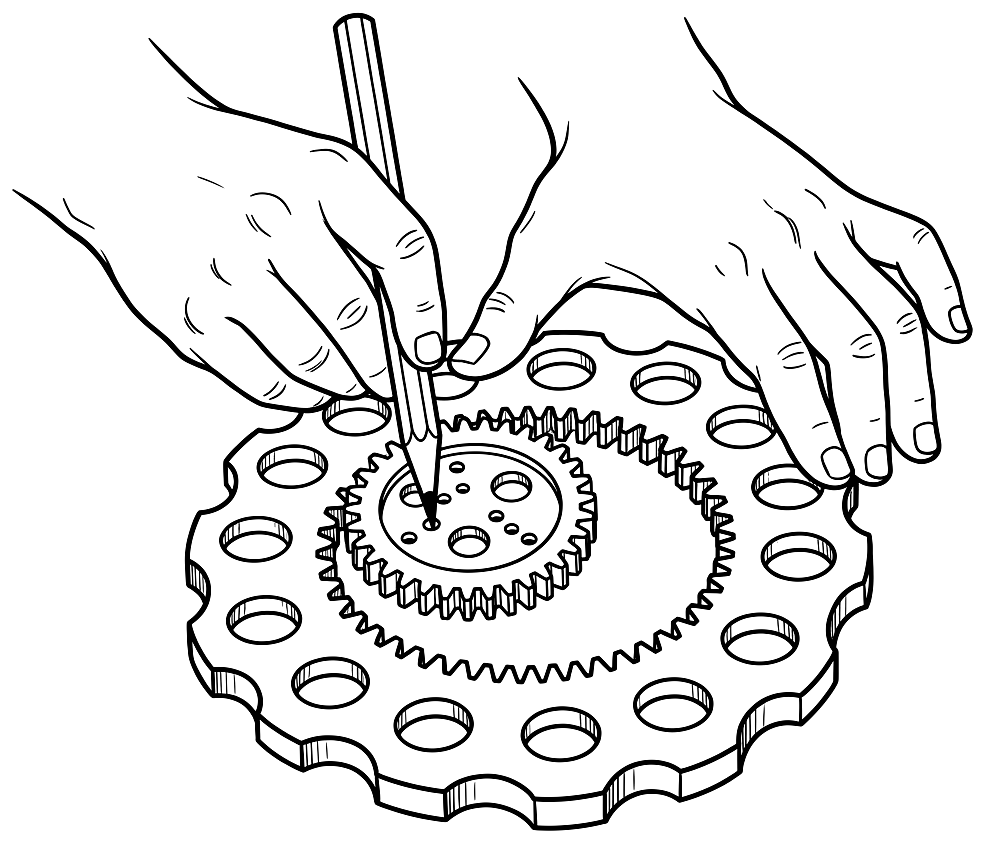
\includegraphics[width=0.48\textwidth]{fig_042_1.png}
  \par\vspace{2pt}
  {\footnotesize (1)}

  \vspace{6pt}
  \begin{minipage}[b]{0.48\textwidth}
    \centering
    \begin{tikzpicture}[scale=1.48, line cap=round, line join=round]
      % (2) 18 瓣四层套叠繁花规花环 (m = 5/18, 1-m = 13/18, k = 13/5 = 2.6)
      \def\om{0.722222}
      \def\kval{2.6}
      \foreach \h/\ph in {0.56/0, 0.51/3, 0.46/6, 0.41/9} {
        \foreach \n in {0,1,2,3,4} {
          \pgfmathsetmacro{\ta}{360*\n}
          \pgfmathsetmacro{\tb}{360*(\n+1)}
          \draw[line width=0.55pt, curveblue!90!black, domain=\ta:\tb, samples=72, variable=\t]
            plot ({\om*cos(\t)+\h*cos(\kval*\t+\ph)},
                  {\om*sin(\t)-\h*sin(\kval*\t+\ph)});
        }
      }
    \end{tikzpicture}
    \par\vspace{2pt}{\footnotesize (2)}
  \end{minipage}
  \hfill
  \begin{minipage}[b]{0.48\textwidth}
    \centering
    \begin{tikzpicture}[scale=1.51, line cap=round, line join=round]
      % (3) 32 瓣细密放射菊花纹 (m = 11/32, 1-m = 21/32, k = 21/11)
      \def\om{0.65625}
      \def\kval{1.9090909}
      \def\h{0.60}
      \foreach \n in {0,1,...,10} {
        \pgfmathsetmacro{\ta}{360*\n}
        \pgfmathsetmacro{\tb}{360*(\n+1)}
        \draw[line width=0.58pt, curveblue!90!black, domain=\ta:\tb, samples=72, variable=\t]
          plot ({\om*cos(\t)+\h*cos(\kval*\t)},
                {\om*sin(\t)-\h*sin(\kval*\t)});
      }
    \end{tikzpicture}
    \par\vspace{2pt}{\footnotesize (3)}
  \end{minipage}

  \vspace{6pt}
  \begin{minipage}[b]{0.48\textwidth}
    \centering
    \begin{tikzpicture}[scale=3.03, line cap=round, line join=round]
      % (4) 28 瓣圆浑菱形编织网球 (m = 19/28, 1-m = 9/28, k = 9/19)
      \def\om{0.3214286}
      \def\kval{0.4736842}
      \def\h{0.305}
      \foreach \n in {0,1,...,18} {
        \pgfmathsetmacro{\ta}{360*\n}
        \pgfmathsetmacro{\tb}{360*(\n+1)}
        \draw[line width=0.58pt, curveblue!90!black, domain=\ta:\tb, samples=56, variable=\t]
          plot ({\om*cos(\t)+\h*cos(\kval*\t)},
                {\om*sin(\t)-\h*sin(\kval*\t)});
      }
    \end{tikzpicture}
    \par\vspace{2pt}{\footnotesize (4)}
  \end{minipage}
  \hfill
  \begin{minipage}[b]{0.48\textwidth}
    \centering
    \begin{tikzpicture}[scale=1.45, line cap=round, line join=round]
      % (5) 3 叶旋转丝带非闭合变幅内摆线 (m = 21/64, 1-m = 43/64, k = 43/21, 绘制 11 圈)
      \def\om{0.671875}
      \def\kval{2.047619}
      \def\h{0.64}
      \foreach \n in {0,1,...,10} {
        \pgfmathsetmacro{\ta}{360*\n}
        \pgfmathsetmacro{\tb}{360*(\n+1)}
        \draw[line width=0.58pt, curveblue!90!black, domain=\ta:\tb, samples=72, variable=\t]
          plot ({\om*cos(\t)+\h*cos(\kval*\t+18)},
                {\om*sin(\t)-\h*sin(\kval*\t+18)});
      }
    \end{tikzpicture}
    \par\vspace{2pt}{\footnotesize (5)}
  \end{minipage}
  \caption*{图\ 42.1}
\end{figure}

\section{两个旋转运动的合成}
\markboth{43. 两个旋转运动的合成}{43. 两个旋转运动的合成}

设有动点 $A$ 绕定点 $O$ 逆时针匀速旋转，角速度为 $\omega$，同时有一个以 $A$ 为圆心的圆盘绕 $A$ 顺时针匀速旋转，角速度为 $\frac{\omega}{m}$，$m>0$。求圆盘边缘上一点 $M$ 的轨迹。

选取计时起点，使当 $t=0$ 时 $M$ 在线段 $OA$ 的延长线上。再选取坐标系，使 $O$ 为原点，并使 $x$ 轴的正半轴与圆 $O$ 的交点 $D$ 恰好是 $t=0$ 时动点 $A$ 所占据的位置。设在时刻 $t$，点 $A$ 和 $M$ 运动到图 43.1 中的位置，这时 $OA$ 延长线与圆 $A$ 的交点为 $E$。设 $OA=l$，$AM=h$，在这段时间内 $M$ 点顺时针转过的角 $\angle EAM=\theta$，则从 $\theta=\frac{\omega}{m}t=\frac{1}{m}\angle DOA$ 得 $\angle DOA=m\theta$，$\overrightarrow{AM}$ 的幅角 $\alpha=m\theta-\theta$。由 $\overrightarrow{OM}=\overrightarrow{OA}+\overrightarrow{AM}$ 得向量 $\overrightarrow{OM}$ 的坐标表示式为
\begin{align*}
  (x,y) &= (l\cos m\theta,\, l\sin m\theta) + (h\cos\alpha,\, h\sin\alpha) \\
        &= \bigl(l\cos m\theta + h\cos(\theta - m\theta), \\
        &\qquad l\sin m\theta - h\sin(\theta - m\theta)\bigr).
\end{align*}
所以 $M$ 点的坐标为
\begin{align*}
  x &= l\cos m\theta + h\cos(\theta - m\theta), \\
  y &= l\sin m\theta - h\sin(\theta - m\theta).
\end{align*}

\noindent
\begin{minipage}[c]{0.52\textwidth}
在图 43.1 中画出的是 $m>1$ 的情形（$\angle AOD > \angle EAM$），容易验证当 $0<m\leqslant 1$ 时仍有同样结果。

\hspace*{2em}若 $m=1$，则
\[
  x = l\cos\theta + h,\quad y = l\sin\theta,
\]
即
\[
  (x-h)^2 + y^2 = l^2,
\]
这时 $M$ 的轨迹是以点 $(h,0)$ 为圆心、$l$ 为半径的圆。
\end{minipage}%
\hfill
\begin{minipage}[c]{0.45\textwidth}
  \centering
  \begin{tikzpicture}[scale=0.80, >=Stealth, line cap=round, line join=round]
    \def\l{1.25}
    \def\h{0.72}
    \def\mth{60}
    \def\th{42}
    \pgfmathsetmacro{\alp}{\mth-\th}
    \coordinate (O) at (0,0);
    \coordinate (D) at (\l, 0);
    \coordinate (A) at ({\l*cos(\mth)}, {\l*sin(\mth)});
    \coordinate (E) at ($ (A) + (\mth:\h) $);
    \coordinate (M) at ($ (A) + (\alp:\h) $);

    % 坐标轴
    \draw[->] (-1.50, 0) -- (1.75, 0) node[below, font=\scriptsize] {$x$};
    \draw[->] (0, -1.50) -- (0, 2.05) node[left, font=\scriptsize] {$y$};

    % 圆 O 与圆 A
    \draw[thick] (O) circle (\l);
    \draw[thick, curveblue] (A) circle (\h);

    % 连线
    \draw (O) -- (E);
    \draw (A) -- (M);
    \draw[thick] (O) -- (M);
    \draw[thin] (A) -- ++(0.74, 0);

    % 角度弧
    \draw (0.28, 0) arc (0:\mth:0.28);
    \node[font=\scriptsize, fill=white, inner sep=0.3pt] at (20:0.48) {$m\theta$};

    \draw ($(A)+(\alp:0.25)$) arc (\alp:\mth:0.25);
    \node[font=\scriptsize] at ($(A)+({\alp+\th/2}:0.42)$) {$\theta$};

    \draw ($(A)+(0:0.40)$) arc (0:\alp:0.40);
    \node[font=\scriptsize] at ($(A)+({\alp/2}:0.56)$) {$\alpha$};

    % 标点与标签
    \fill (O) circle (1.2pt) node[below left=-1pt, font=\scriptsize] {$O$};
    \fill (D) circle (1.2pt) node[below right=-1pt, font=\scriptsize] {$D$};
    \fill (A) circle (1.3pt) node[above left=-1pt, font=\scriptsize] {$A$};
    \fill (E) circle (1.2pt) node[above, font=\scriptsize] {$E$};
    \fill (M) circle (1.3pt) node[right, font=\scriptsize] {$M$};
  \end{tikzpicture}
  \captionof*{figure}{图\ 43.1}
\end{minipage}

若 $m<1$，则可令 $l=R-mR$，得
\begin{align*}
  x &= (R-mR)\cos m\theta + h\cos(\theta - m\theta), \\
  y &= (R-mR)\sin m\theta - h\sin(\theta - m\theta),
\end{align*}
式中 $R$、$h$ 为正数，$0<m<1$，因而轨迹为内摆线或变幅内摆线，视 $h=mR$ 或 $h\neq mR$ 而定（参考第 35 节）。

若 $m>1$，则可令
\[
  m-1=m_1,\qquad l=h_1,\qquad h=R+m_1 R,
\]
这里 $R$、$h_1$ 和 $m_1$ 都是正数，并且曲线方程化成
\begin{align*}
  x &= h_1\cos(\theta + m_1\theta) + (R+m_1 R)\cos m_1\theta, \\
  y &= h_1\sin(\theta + m_1\theta) + (R+m_1 R)\sin m_1\theta,
\end{align*}
所以这时轨迹是外摆线族曲线（参考第 34 节）。

\section{用三把车刀切削正六边形零件}
\markboth{44. 用三把车刀切削正六边形零件}{44. 用三把车刀切削正六边形零件}

在各种机械中用到很多螺丝钉和螺丝帽，大多数螺丝帽的侧面都具有正六边形的轮廓。在经常生产大批同一规格螺丝帽的地方，只要做一个专门的模具，就能很方便地在螺帽半成品上切削出有固定大小的正六边形轮廓。但是也有一些工厂需要各种不同规格的六角螺帽，而同一规格的需要量又不大，犯不着做很多种不同的模具。为了充分挖掘设备的潜力，提高生产效率，可以设法在车床上加上一个专用夹具，用三把车刀来切削各种小螺丝帽侧面的正六边形轮廓。

螺丝帽的半成品，外部轮廓是一个圆，最后需要保留的轮廓是这个圆的内接正六边形。在车床的主轴上装一个大圆盘，叫做刀盘，在刀盘的圆周上每隔 $120^\circ$ 装一把车刀，共装三把，使刀头沿刀盘的半径方向伸出到刀盘外面，注意使三把车刀露出刀盘的部分的长度相同。做一个夹具，使工件的圆周与刀盘圆周在同一平面内，两个圆心间的距离可以调节，并且当刀盘旋转时，通过齿轮带动工件沿相同方向旋转，刀盘转速是工件转速的二倍。

从图 44.1 中可以看出，用三把车刀切削正六边形的过程，就像用三颗牙齿轮流啃苹果一样，先是第一把车刀 $M$ 在工件圆盘上“啃”掉 $60^\circ$ 的圆弧，得到圆内接正六边形的一边，接着第二把车刀 $N$ 赶上来“啃”出第二边，如此继续。每把车刀“啃”出面对面的两边，因而三把车刀合作，切削出整个正六边形的轮廓。当然，金属比苹果硬得多，不是那么容易啃的，所以实际切削时，不能像图 44.1 那样一刀就切削出一边来，而只能逐步缩短圆心距 $OA$，分若干次进刀，每次进刀后只切削掉薄薄的一层。

\begin{figure}[htbp]
  \centering
  % 公共参数与绘制单个状态的命令
  % #1: 刀盘顺时针转角 (相对于 M 在 196 deg), #2: 工件绘制代码
  \newcommand{\hexpanel}[2]{%
    \begin{tikzpicture}[scale=0.90, >=Stealth, line cap=round, line join=round]
      \def\rw{0.38}
      \def\rd{0.72}
      \def\htip{0.84}
      \def\lOA{1.17}
      \def\phiA{#1}
      \pgfmathsetmacro{\hexrot}{-(\phiA - 16)/2}
      \coordinate (O) at (0,0);
      \coordinate (A) at (\lOA, 0);

      % 中心十字线
      \draw[densely dash dot, thin] (-0.54, 0) -- (2.06, 0);
      \draw[densely dash dot, thin] (0, -0.54) -- (0, 0.54);
      \draw[densely dash dot, thin] (\lOA, -0.90) -- (\lOA, 0.90);

      % 工件内部浅虚线内接正六边形参考线（随工件同步顺时针旋转）
      \draw[densely dashed, thin, black!45]
        ({30+\hexrot}:\rw) -- ({90+\hexrot}:\rw) -- ({150+\hexrot}:\rw)
        -- ({210+\hexrot}:\rw) -- ({270+\hexrot}:\rw) -- ({330+\hexrot}:\rw) -- cycle;

      % 工件轮廓
      #2

      % 刀盘圆
      \draw[thick] (A) circle (\rd);

      % 三把车刀 (M, N, P 顺时针相隔 120 度)
      \pgfmathsetmacro{\angM}{196 - \phiA}
      \pgfmathsetmacro{\angN}{196 + 120 - \phiA}
      \pgfmathsetmacro{\angP}{196 - 120 - \phiA}
      \foreach \ang/\lbl in {\angM/M, \angN/N, \angP/P} {
        \coordinate (Tb1) at ($(A)+({\ang-5}:\rd)$);
        \coordinate (Tb2) at ($(A)+({\ang+5}:\rd)$);
        \coordinate (Ttp) at ($(A)+(\ang:\htip)$);
        \draw[thick, fill=white] (Tb1) -- (Ttp) -- (Tb2) -- cycle;
        % 若刀尖正在左侧 O 处切削 (165..205 deg)，标签置于刀尖外上或外下侧，避免落入圆 O 内
        \pgfmathtruncatemacro{\side}{(\ang > 165 && \ang < 188) ? 1 : ((\ang >= 188 && \ang < 210) ? -1 : 0)}
        \ifnum\side=1
          \node[font=\scriptsize, fill=white, inner sep=0.4pt]
            at ($(A)+(153:{\htip+0.19})$) {$\lbl$};
        \else\ifnum\side=-1
          \node[font=\scriptsize, fill=white, inner sep=0.4pt]
            at ($(A)+(214:{\htip+0.19})$) {$\lbl$};
        \else
          \node[font=\scriptsize, fill=white, inner sep=0.4pt]
            at ($(A)+(\ang:{\htip+0.18})$) {$\lbl$};
        \fi\fi
      }

      % 旋转箭头 omega 与 2omega (均为顺时针)
      \draw[->, thin] ($(O)+(225:0.49)$) arc (225:155:0.49);
      \node[font=\tiny] at ($(O)+(220:0.63)$) {$\omega$};
      \draw[->, thin] ($(A)+(252:0.54)$) arc (252:208:0.54);
      \node[font=\tiny, fill=white, inner sep=0.4pt] at ($(A)+(230:0.39)$) {$2\omega$};

      \fill (O) circle (0.9pt) node[below left=-2pt, font=\scriptsize] {$O$};
      \fill (A) circle (0.9pt) node[below right=-2pt, font=\scriptsize] {$A$};
    \end{tikzpicture}%
  }

  \begin{minipage}[b]{0.48\textwidth}
    \centering
    \hexpanel{0}{%
      \draw[thick, curveblue] (O) circle (\rw);
    }
  \end{minipage}
  \hfill
  \begin{minipage}[b]{0.48\textwidth}
    \centering
    \hexpanel{16}{%
      \draw[densely dashed, thin, black!40] (O) circle (\rw);
      \draw[thick, curveblue] (-30:\rw) -- ({\rw*cos(30)}, 0) -- (0:\rw) arc (0:330:\rw) -- cycle;
    }
  \end{minipage}

  \vspace{4pt}
  \begin{minipage}[b]{0.48\textwidth}
    \centering
    \hexpanel{36}{%
      \draw[densely dashed, thin, black!40] (O) circle (\rw);
      \draw[thick, curveblue] (20:\rw) arc (20:320:\rw) -- cycle;
    }
  \end{minipage}
  \hfill
  \begin{minipage}[b]{0.48\textwidth}
    \centering
    \hexpanel{76}{%
      \draw[densely dashed, thin, black!40] (O) circle (\rw);
      \draw[thick, curveblue] (0:\rw) arc (0:300:\rw) -- cycle;
    }
  \end{minipage}

  \vspace{4pt}
  \begin{minipage}[b]{0.48\textwidth}
    \centering
    \hexpanel{120}{%
      \draw[densely dashed, thin, black!40] (O) circle (\rw);
      \draw[thick, curveblue] (-22:\rw) arc (-22:278:\rw) -- cycle;
    }
  \end{minipage}
  \hfill
  \begin{minipage}[b]{0.48\textwidth}
    \centering
    \hexpanel{136}{%
      \draw[densely dashed, thin, black!40] (O) circle (\rw);
      \draw[thick, curveblue] (-90:\rw) -- (-30:\rw) -- ({\rw*cos(30)}, 0) -- (0:\rw) arc (0:270:\rw) -- cycle;
    }
  \end{minipage}
  \caption*{图\ 44.1}
\end{figure}

从数学角度来看，旋转的车刀在旋转的工件上切削出曲线轮廓，相当于旋转的笔在旋转的纸上画曲线。刀尖 $M$ 相当于笔尖，工件圆盘相当于一张白纸。要能看清旋转的“笔”在旋转的“纸”上画出什么曲线，观察者必须设想自己能够随着“纸”一起绕 $O$ 点旋转。在这样的观察者眼中，就会觉得似乎不是工件绕 $O$ 点以角速度 $\omega$ 顺时针旋转，刀盘中心 $A$ 不动，而好像是工件不动，刀盘中心 $A$ 以角速度 $\omega$ 绕 $O$ 点逆时针旋转。与此同时，刀尖 $M$ 又以角速度 $2\omega$ 绕 $A$ 点顺时针旋转。这样就归结成第 43 节中已经讨论过的情形（这里 $m=\frac{1}{2}$），因而刀尖 $M$ 在工件上切削出的轮廓曲线的方程是
\begin{align*}
  x &= l\cos\frac{\theta}{2} + h\cos\left(\theta - \frac{\theta}{2}\right), \\
  y &= l\sin\frac{\theta}{2} - h\sin\left(\theta - \frac{\theta}{2}\right),
\end{align*}
其中 $l=OA$，$h=AM$，$\frac{\theta}{2}=\omega t$。将上述方程化简，得到
\begin{align*}
  x &= (l+h)\cos\frac{\theta}{2}, \\
  y &= (l-h)\sin\frac{\theta}{2},
\end{align*}
即
\[
  \frac{x^2}{(l+h)^2} + \frac{y^2}{(l-h)^2} = 1.
\]

\noindent
\begin{minipage}[c]{0.44\textwidth}
  \centering
  \begin{tikzpicture}[scale=0.88, line cap=round, line join=round]
    \def\aell{1.45}
    \def\bell{0.19}
    \pgfmathsetmacro{\lOA}{(\aell+\bell)/2}
    \pgfmathsetmacro{\htip}{(\aell-\bell)/2}
    \def\rd{0.50}
    \pgfmathsetmacro{\hexr}{\bell/cos(30)}

    % 中心线
    \draw[densely dash dot, thin] (-1.45, 0) -- (1.55, 0);
    \draw[densely dash dot, thin] (\lOA, -0.75) -- (\lOA, 0.75);

    % 三个错开 60 度的扁椭圆 (长轴分别沿 90, 30, 150 度)
    \foreach \rot in {0, 60, -60} {
      \draw[densely dashed, thick, curveblue, rotate=\rot] (0,0) ellipse ({\bell} and {\aell});
    }

    % 中心正六边形“核”
    \fill[pattern=north east lines, pattern color=mutedgray]
      (30:\hexr) -- (90:\hexr) -- (150:\hexr) -- (210:\hexr) -- (270:\hexr) -- (330:\hexr) -- cycle;
    \draw[thick]
      (30:\hexr) -- (90:\hexr) -- (150:\hexr) -- (210:\hexr) -- (270:\hexr) -- (330:\hexr) -- cycle;

    % 刀盘圆及三把车刀 (位于 180, 60, -60 度)
    \coordinate (A) at (\lOA, 0);
    \draw[thick] (A) circle (\rd);
    \foreach \ang in {180, 60, -60} {
      \draw[thick, fill=white]
        ($(A)+({\ang-6}:\rd)$) -- ($(A)+(\ang:\htip)$) -- ($(A)+({\ang+6}:\rd)$) -- cycle;
    }
  \end{tikzpicture}
  \captionof*{figure}{图\ 44.2}
\end{minipage}%
\hfill
\begin{minipage}[c]{0.53\textwidth}
所以刀尖 $M$ 在工件的平面上画出一个椭圆（图 44.2）。这个椭圆的短半轴 $l-h$ 远远小于长半轴 $l+h$，因而又扁又长，所以这椭圆靠近中心 $O$ 的两小段弧非常接近于一对平行直线上的线段，可作为正六边形的一双对边。三把互相错开 $120^\circ$ 的车刀，画出三个互相错开 $60^\circ$ 的很扁的椭圆，恰好提供了正六边形的三双对边。
\end{minipage}

\section{用一把车刀切削正多边形零件}
\markboth{45. 用一把车刀切削正多边形零件}{45. 用一把车刀切削正多边形零件}

在第 44 节中已经证明了，如果让工件和刀盘在同一平面内沿相同方向转动，并且工件转速是刀盘转速的 $m$ 倍，那么装在刀盘上的任一把车刀的刀尖 $M$ 在工件平面内的轨迹，可用下面的方程表示：
\begin{align*}
  x &= l\cos m\theta + h\cos(\theta - m\theta), \\
  y &= l\sin m\theta - h\sin(\theta - m\theta),
\end{align*}
这里 $l$ 是工件中心与刀盘中心的距离，$h$ 是刀尖 $M$ 到刀盘中心的距离，$0<h<l$，并且 $l-h$ 比 $l+h$ 小得多。在第 44 节中选用 $m=\frac{1}{2}$，因而刀尖在工件平面内的轨迹是狭长的椭圆，三个椭圆才能围出一个六边形区域来。所以选用 $m=\frac{1}{2}$ 时必须用三把车刀才能切削出正六边形。

如果我们在夹具上调换传动齿轮，因而改变工件转速与刀盘转速的比值 $m$，其余条件不变，那么刀尖的轨迹就会变成其它的内摆线族或外摆线族曲线，这时往往一条曲线就能围出一个多边形的“核”来，因而只用一把车刀就能切削正多边形工件。

\begin{figure}[htbp]
  \centering
  \begin{minipage}[b]{0.24\textwidth}
    \centering
    \begin{tikzpicture}[scale=0.58]
      \def\m{1/3}
      \def\h{0.76}
      \draw[thick, curveblue, domain=0:1080, samples=260, variable=\t]
        plot ({cos(\m*\t)+\h*cos((1-\m)*\t)},
              {sin(\m*\t)-\h*sin((1-\m)*\t)});
    \end{tikzpicture}
    \caption*{图\ 45.1}
  \end{minipage}
  \hfill
  \begin{minipage}[b]{0.24\textwidth}
    \centering
    \begin{tikzpicture}[scale=0.58]
      \def\m{3/5}
      \def\h{0.76}
      \draw[thick, curveblue, domain=0:1800, samples=340, variable=\t]
        plot ({cos(\m*\t)+\h*cos((1-\m)*\t)},
              {sin(\m*\t)-\h*sin((1-\m)*\t)});
    \end{tikzpicture}
    \caption*{图\ 45.2}
  \end{minipage}
  \hfill
  \begin{minipage}[b]{0.24\textwidth}
    \centering
    \begin{tikzpicture}[scale=0.58]
      \def\m{1/6}
      \def\h{0.68}
      \draw[thick, curveblue, domain=0:2160, samples=360, variable=\t]
        plot ({cos(\m*\t)+\h*cos((1-\m)*\t)},
              {sin(\m*\t)-\h*sin((1-\m)*\t)});
    \end{tikzpicture}
    \caption*{图\ 45.3}
  \end{minipage}
  \hfill
  \begin{minipage}[b]{0.24\textwidth}
    \centering
    \begin{tikzpicture}[scale=0.58]
      \def\m{3/7}
      \def\h{0.78}
      \draw[thick, curveblue, domain=0:2520, samples=420, variable=\t]
        plot ({cos(\m*\t)+\h*cos((1-\m)*\t)},
              {sin(\m*\t)-\h*sin((1-\m)*\t)});
    \end{tikzpicture}
    \caption*{图\ 45.4}
  \end{minipage}
\end{figure}

在图 45.1 $\sim$ 45.4 中分别画出 $m=\frac{1}{3}$、$\frac{3}{5}$、$\frac{1}{6}$ 和 $\frac{3}{7}$ 的情形\footnote{重排校订：原书图 45.1（$m=\frac{1}{3}$）将极半径极大值（顶点）误绘于正左方，与参数方程 $\theta=0$ 时 $(x,y)=(l+h,0)$ 位于正右方的方位相差 $180^\circ$；本版据参数方程真实方位统一重绘图 45.1～45.4。}，这些曲线的中心都有一个多边形“核”，多边形的边数顺次是 $3$、$5$、$6$、$7$。所以，如果让工件转速是刀盘转速的 $\frac{1}{6}$，只要用一把车刀就能切削螺丝帽侧面的正六边形。而如果想切削正五边形的零件，只要改变转速比，使工件转速是刀盘转速的 $\frac{3}{5}$ 就行了。

一般地，如果想用一把车刀切削正 $n$ 边形，应该怎样选择 $m$ 的值呢？

由于采用齿轮传动，转速比是两个正整数的比，因而比值 $m$ 必为有理数。把 $m$ 表示成既约分数 $\frac{q}{p}$，并且把 $m=\frac{q}{p}$ 代入曲线方程，得到
\begin{align*}
  x &= l\cos\frac{q\theta}{p} + h\cos\frac{(p-q)\theta}{p}, \\
  y &= l\sin\frac{q\theta}{p} - h\sin\frac{(p-q)\theta}{p}.
\end{align*}
因为 $q$ 与 $p$ 互质，所以 $p-q$ 也与 $p$ 互质。由此知道 $2p\pi$ 是函数 $\cos\frac{q\theta}{p}$、$\sin\frac{q\theta}{p}$、$\cos\frac{(p-q)\theta}{p}$ 和 $\sin\frac{(p-q)\theta}{p}$ 的周期，因而 $x$ 和 $y$ 也都是周期为 $2p\pi$ 的函数。只要让参数 $\theta$ 在范围 $0\leqslant\theta<2p\pi$ 内变化，就能得到整个曲线。

从曲线方程又得到
\[
  x^2+y^2 = l^2+h^2+2lh\cos\left(\frac{q\theta}{p}+\frac{(p-q)\theta}{p}\right),
\]
即
\begin{align*}
  x^2+y^2 &= l^2+h^2+2lh\cos\theta \\
          &\geqslant l^2+h^2-2lh \\
          &= (l-h)^2.
\end{align*}
由于 $0<h<l$，所以
\[
  \sqrt{x^2+y^2} \geqslant l-h,
\]
等号当且仅当 $\cos\theta=-1$ 时成立。$\sqrt{x^2+y^2}$ 是曲线上的点到坐标原点的距离，使它取得极小值 $l-h$ 的点，是曲线上离它的中心 $O$ 最近的点，即多边形“核”的某一边的中点。因而，多边形的边数 $n$，恰好等于曲线上使 $\sqrt{x^2+y^2}$ 取极小值的点的个数，即在范围 $0\leqslant\theta<2p\pi$ 内满足 $\cos\theta=-1$ 的 $\theta$ 值的个数。满足这些条件的 $\theta$ 值是
\[
  \theta = \pi + 2k\pi,\quad (k=0,\, 1,\, \cdots,\, p-1)
\]
共有 $p$ 个。所以 $n=p$。

这样一来，我们就得到一个很方便的计算法则：要想用一把车刀切削正 $n$ 边形的小零件，只要选取转速比，使工件的转速是刀盘转速的 $\frac{q}{n}$ 倍，这里 $\frac{q}{n}$ 是一个既约分数。

例如，想用一把车刀切削出正六边形轮廓，$m=\frac{q}{n}=\frac{q}{6}$，$q$ 取 $1$ 或 $5$ 时，$\frac{1}{6}$ 和 $\frac{5}{6}$ 都是既约分数，所以只要使工件转速与刀盘转速的比为 $1:6$ 或 $5:6$，都可以达到目的。

\section{正方形的渐伸线}
\markboth{46. 正方形的渐伸线}{46. 正方形的渐伸线}

蚊香盒的底面是一个正方形，拿一张旧报纸放在桌上，把蚊香盒放在报纸上，盒底的轮廓就在报纸上显示出一个正方形，记为 $ABCD$，并设其边长为 $a$。再取一根细线绕到蚊香盒外侧的下部，线的一端结上一支铅笔，使笔尖正好位于正方形的一个顶点 $A$ 处。然后手执铅笔拉紧细线，并且把线从盒底上逐渐松开，铅笔就在报纸上画出一条螺旋形曲线，这条曲线叫做正方形的渐伸线（图 46.1）。

\begin{wrapfigure}[11]{l}{0.43\textwidth}
  \centering
  \vspace{-4pt}
  \begin{tikzpicture}[scale=0.90, line cap=round, line join=round]
    \def\a{0.38}
    \coordinate (D) at (0, 0);
    \coordinate (C) at (\a, 0);
    \coordinate (B) at (\a, \a);
    \coordinate (A) at (0, \a);
    \coordinate (E) at (\a, {2*\a});
    \coordinate (F) at ({3*\a}, 0);
    \coordinate (G) at (0, {-3*\a});
    \coordinate (H) at ({-4*\a}, \a);

    % 正方形 ABCD
    \draw[thick] (D) -- (C) -- (B) -- (A) -- cycle;

    % 虚线辅助线
    \draw[densely dashed] (B) -- (E);
    \draw[densely dashed] (C) -- (F);
    \draw[densely dashed] (D) -- (G);
    \draw[densely dashed] (A) -- (H);

    % 渐伸线四段圆弧
    \draw[very thick, curveblue]
      (A) arc (180:90:\a)
          arc (90:0:{2*\a})
          arc (0:-90:{3*\a})
          arc (-90:-180:{4*\a});

    % 顶点与字母标签
    \fill (A) circle (1.2pt) node[above left=-1pt, font=\scriptsize] {$A$};
    \fill (B) circle (1.2pt) node[right, font=\scriptsize] {$B$};
    \fill (C) circle (1.2pt) node[below right=-1pt, font=\scriptsize] {$C$};
    \fill (D) circle (1.2pt) node[left, font=\scriptsize] {$D$};
    \node[above, font=\scriptsize] at (E) {$E$};
    \node[right, font=\scriptsize] at (F) {$F$};
    \node[below, font=\scriptsize] at (G) {$G$};
    \node[left, font=\scriptsize] at (H) {$H$};
  \end{tikzpicture}
  \caption*{图\ 46.1}
\end{wrapfigure}

根据作法知道，正方形的渐伸线是由一些不同半径的圆弧光滑连接而成的。例如在图 46.1 中，$\arc{AE}$ 的圆心是 $B$，半径是 $a$；$\arc{EF}$ 的圆心是 $C$，半径是 $2a$；$\arc{FG}$ 的圆心是 $D$，半径是 $3a$，等等。

还可用类似的方法画出圈数更多的螺旋形曲线，而且通过适当选择各个圆心的位置，螺旋形曲线的形状也可以千变万化。例如图 46.2 中画出的螺旋形曲线，也是由一些圆弧光滑地连接而成的，各段圆弧的圆心顺次是 $A$、$B$、$C$、$D$ 等等。这种画螺旋形曲线的方法非常简便，在机械制图和建筑工程中常被采用。

\begin{figure}[htbp]
  \centering
  \begin{tikzpicture}[scale=1.12, line cap=round, line join=round]
    % 宽阔平放的饱满蜗壳形四段圆弧螺旋，圆心顺次为 A, B, C, D
    \def\hB{0.72}
    \def\w{0.38}
    \def\hD{0.38}
    \pgfmathsetmacro{\rone}{2*\hB + \w}
    \pgfmathsetmacro{\rtwo}{\rone - \hB}
    \pgfmathsetmacro{\rthree}{\rtwo - \w}
    \pgfmathsetmacro{\rfour}{\hD}

    \coordinate (A) at (0, 0);
    \coordinate (B) at (0, \hB);
    \coordinate (C) at (\w, \hB);
    \coordinate (D) at (\w, \hD);

    % 水平底边及各段圆弧衔接半径辅助线
    \draw[thin] (-\rone, 0) -- (\w, 0);
    \draw[densely dashed, black!65] (A) -- (0, \rone);
    \draw[densely dashed, black!65] (B) -- (\rtwo, \hB);
    \draw[densely dashed, black!65] (C) -- (\w, 0);
    \draw[densely dashed, black!65] (D) -- (0, \hD);

    % 顺次以 A, B, C, D 为圆心光滑连接的四段 90° 圆弧螺旋
    \draw[very thick, curveblue]
      (-\rone, 0) arc (180:90:\rone)
                  arc (90:0:\rtwo)
                  arc (0:-90:\rthree)
                  arc (-90:-180:\rfour);

    % 圆心标记（全部置于清晰空白处，不压任何虚线与曲线）
    \fill (A) circle (1.1pt) node[below=1.5pt, font=\scriptsize] {$A$};
    \fill (B) circle (1.1pt) node[left=1.5pt, font=\scriptsize] {$B$};
    \fill (C) circle (1.1pt) node[above=1.5pt, font=\scriptsize] {$C$};
    \fill (D) circle (1.1pt) node[right=1.5pt, font=\scriptsize] {$D$};
  \end{tikzpicture}
  \caption*{图\ 46.2}
\end{figure}

\section{圆的渐伸线}
\markboth{47. 圆的渐伸线}{47. 圆的渐伸线}

在桌上铺一张白纸，纸上放一只大口瓶的盖子，并且把一端系有铅笔的细线绕在瓶盖的圆周外面，手执铅笔拉紧细线，让线逐渐放开伸直，铅笔就在纸上画出一条螺旋形曲线，这条曲线叫做圆的渐伸线（图 47.1）。瓶盖映在纸上的圆形轮廓，叫做这条曲线的基圆。在工厂里和在制图学课本里，习惯于把这种曲线叫做圆的渐开线。

\begin{figure}[htbp]
  \centering
  \begin{minipage}[b]{0.46\textwidth}
    \centering
    \begin{tikzpicture}[scale=0.88, >=Stealth, line cap=round, line join=round]
      % 瓶盖（透视圆柱体，底面椭圆中心在 (0, 0.26)，半轴 rx=0.28, ry=0.10）
      \def\rx{0.28}
      \def\ry{0.10}
      \def\h{0.16}
      \def\yc{0.26}

      % 透视展开的渐伸线（严格保持与底面椭圆相同的透视投影比例 rx, ry）
      \draw[very thick, curveblue, domain=0:345, samples=140, variable=\t]
        plot ({\rx*(cos(\t)+(\t*pi/180)*sin(\t))},
              {\yc+\ry*(sin(\t)-(\t*pi/180)*cos(\t))});

      % 瓶盖侧面与底面可见轮廓
      \draw[thick, fill=white] (-\rx, {\yc+\h}) -- (-\rx, \yc)
        arc (180:360:{\rx} and {\ry}) -- (\rx, {\yc+\h});
      \draw[densely dashed] (-\rx, \yc) arc (180:0:{\rx} and {\ry});
      \draw[thick, fill=white] (0, {\yc+\h}) ellipse ({\rx} and {\ry});

      % 位置 1（虚线铅笔，t = 205 deg，左上方切线严格等于弧长）
      \pgfmathsetmacro{\ta}{205}
      \pgfmathsetmacro{\tar}{\ta*pi/180}
      \coordinate (Ba) at ({\rx*cos(\ta)}, {\yc+\ry*sin(\ta)});
      \coordinate (Pa) at ({\rx*(cos(\ta)+\tar*sin(\ta))}, {\yc+\ry*(sin(\ta)-\tar*cos(\ta))});
      \draw[densely dashed] (Ba) -- (Pa);
      \draw[densely dashed] (Pa) -- ++(-0.06, 0.18) -- ++(0, 0.25) -- ++(0.12, 0) -- ++(0, -0.25) -- cycle;

      % 位置 2（虚线铅笔，t = 272 deg，左下方切线严格等于弧长）
      \pgfmathsetmacro{\tb}{272}
      \pgfmathsetmacro{\tbr}{\tb*pi/180}
      \coordinate (Bb) at ({\rx*cos(\tb)}, {\yc+\ry*sin(\tb)});
      \coordinate (Pb) at ({\rx*(cos(\tb)+\tbr*sin(\tb))}, {\yc+\ry*(sin(\tb)-\tbr*cos(\tb))});
      \draw[densely dashed] (Bb) -- (Pb);
      \draw[densely dashed] (Pb) -- ++(-0.06, 0.18) -- ++(0, 0.25) -- ++(0.12, 0) -- ++(0, -0.25) -- cycle;

      % 位置 3（当前实线铅笔，t = 345 deg，右下方切线严格等于弧长）
      \pgfmathsetmacro{\tc}{345}
      \pgfmathsetmacro{\tcr}{\tc*pi/180}
      \coordinate (Bc) at ({\rx*cos(\tc)}, {\yc+\ry*sin(\tc)});
      \coordinate (Pc) at ({\rx*(cos(\tc)+\tcr*sin(\tc))}, {\yc+\ry*(sin(\tc)-\tcr*cos(\tc))});
      \draw[thick] (Bc) -- (Pc);
      \draw[thick, fill=white] (Pc) -- ++(-0.07, 0.20) -- ++(0, 0.26) -- ++(0.14, 0) -- ++(0, -0.26) -- cycle;
      \draw[thin] ($(Pc)+(-0.07, 0.20)$) -- ($(Pc)+(-0.025, 0.18)$) -- ($(Pc)+(0.025, 0.20)$) -- ($(Pc)+(0.07, 0.20)$);
      \draw[thin] ($(Pc)+(-0.025, 0.18)$) -- ($(Pc)+(-0.025, 0.46)$);
      \draw[thin] ($(Pc)+(0.025, 0.20)$) -- ($(Pc)+(0.025, 0.46)$);

      % 方向箭头
      \draw[->, thick] (0.48, 0.56) arc (25:65:0.45);
      \draw[->, thick] (-1.22, -0.18) arc (205:240:0.95);
    \end{tikzpicture}
    \caption*{图\ 47.1}
  \end{minipage}
  \hfill
  \begin{minipage}[b]{0.50\textwidth}
    \centering
    \begin{tikzpicture}[scale=0.90, >=Stealth, line cap=round, line join=round]
      \def\a{0.76}
      \def\phideg{56}
      \pgfmathsetmacro{\phirad}{\phideg*pi/180}
      \coordinate (O) at (0,0);
      \coordinate (A) at (\a, 0);
      \coordinate (B) at ({\a*cos(\phideg)}, {\a*sin(\phideg)});
      \coordinate (P) at ({\a*(cos(\phideg)+\phirad*sin(\phideg))},
                          {\a*(sin(\phideg)-\phirad*cos(\phideg))});

      % 坐标轴
      \draw[->] (-1.05, 0) -- (1.85, 0) node[below, font=\scriptsize] {$x$};
      \draw[->] (0, -1.05) -- (0, 2.00) node[left, font=\scriptsize] {$y$};

      % 基圆与渐伸线
      \draw[thick] (O) circle (\a);
      \draw[very thick, curveblue, domain=0:118, samples=80, variable=\t]
        plot ({\a*(cos(\t)+(\t*pi/180)*sin(\t))},
              {\a*(sin(\t)-(\t*pi/180)*cos(\t))});

      % 矢量与切线
      \draw[->] (O) -- (B);
      \draw[->] (B) -- (P);
      \draw[->] (O) -- (P);

      % 直角标志 at B
      \coordinate (Br) at ($(B)+({\phideg-180}:0.12)$);
      \coordinate (Bt) at ($(B)+({\phideg-90}:0.12)$);
      \coordinate (Bc) at ($(Br)+(Bt)-(B)$);
      \draw (Br) -- (Bc) -- (Bt);

      % B 处角 phi 与 phi - pi/2 (错开半径避免遮挡)
      \draw (B) -- ++({\phideg}:0.48);
      \draw (B) -- ++(0.68, 0);
      \draw ($(B)+(0:0.24)$) arc (0:\phideg:0.24);
      \node[font=\scriptsize] at ($(B)+({\phideg/2}:0.39)$) {$\phi$};

      \draw ($(B)+(0:0.42)$) arc (0:{\phideg-90}:0.42);
      \draw[thin] ($(B)+({(\phideg-90)/2}:0.42)$) -- ($(B)+(0.86, 0.34)$)
        node[right, font=\scriptsize] {$\phi-\dfrac{\pi}{2}$};

      % O 处角 phi
      \draw (0.24, 0) arc (0:\phideg:0.24);
      \node[font=\scriptsize] at ({\phideg/2}:0.38) {$\phi$};

      % 标点与标签
      \fill (O) circle (1.2pt) node[below left=-1pt, font=\scriptsize] {$O$};
      \fill (A) circle (1.2pt) node[below right=-1pt, font=\scriptsize] {$A$};
      \fill (B) circle (1.3pt) node[above left=-1pt, font=\scriptsize] {$B$};
      \fill (P) circle (1.3pt) node[right, font=\scriptsize] {$P(x,y)$};
    \end{tikzpicture}
    \caption*{图\ 47.2}
  \end{minipage}
\end{figure}

如图 47.2，设 $P(x,y)$ 是圆的渐伸线上的任意点，$B$ 是基圆 $O$ 上的对应点，$A$ 是圆的渐伸线与圆 $O$ 的交点。根据圆的渐伸线的画法知道，图中的线段 $BP$ 是把 $\arc{BA}$ 拉直而成的，并且 $PB$ 是圆 $O$ 的切线。取 $O$ 为坐标原点，$OA$ 为 $x$ 轴正方向。设圆 $O$ 的半径为 $a$，$\angle AOB=\phi$，则 $\overrightarrow{BP}$ 的幅角为 $\phi-\frac{\pi}{2}$，由 $\overrightarrow{OP}=\overrightarrow{OB}+\overrightarrow{BP}$ 得向量 $\overrightarrow{OP}$ 的坐标表示式为
\begin{align*}
  (x,y) &= (a\cos\phi,\, a\sin\phi) \\
        &\quad + \left(a\phi\cos\left(\phi-\frac{\pi}{2}\right),\, a\phi\sin\left(\phi-\frac{\pi}{2}\right)\right) \\
        &= (a\cos\phi+a\phi\sin\phi,\, a\sin\phi-a\phi\cos\phi).
\end{align*}
所以圆的渐伸线的参数方程为
\begin{align*}
  x &= a(\cos\phi+\phi\sin\phi), \\
  y &= a(\sin\phi-\phi\cos\phi).
\end{align*}

\section{圆的渐伸线的切线和法线}
\markboth{48. 圆的渐伸线的切线和法线}{48. 圆的渐伸线的切线和法线}

\noindent
\begin{minipage}[c]{0.45\textwidth}
  \centering
  \begin{tikzpicture}[scale=1.00, >=Stealth, line cap=round, line join=round]
    \def\a{0.75}
    \def\phideg{58}
    \pgfmathsetmacro{\phirad}{\phideg*pi/180}
    \coordinate (O) at (0,0);
    \coordinate (A) at (\a, 0);
    \coordinate (B) at ({\a*cos(\phideg)}, {\a*sin(\phideg)});
    \coordinate (P) at ({\a*(cos(\phideg)+\phirad*sin(\phideg))},
                        {\a*(sin(\phideg)-\phirad*cos(\phideg))});
    % C 为从 O 向切线 PT 所作垂线的垂足: OC 方向为 phideg - 90, 长度 a*phirad
    \coordinate (C) at ({\a*\phirad*cos(\phideg-90)}, {\a*\phirad*sin(\phideg-90)});
    % T 在 PT 延长线上
    \coordinate (T) at ($(P)+(\phideg:0.52)$);

    % 坐标轴
    \draw[->] (-0.95, 0) -- (1.72, 0) node[below, font=\scriptsize] {$x$};
    \draw[->] (0, -0.95) -- (0, 1.32) node[left, font=\scriptsize] {$y$};

    % 基圆与渐伸线
    \draw[thick] (O) circle (\a);
    \draw[very thick, curveblue, domain=0:94, samples=60, variable=\t]
      plot ({\a*(cos(\t)+(\t*pi/180)*sin(\t))},
            {\a*(sin(\t)-(\t*pi/180)*cos(\t))});

    % 线段 OB, BP, OC, 切线 CT（phi=58° 使 OB 远离 y 轴、OC 更陡，a 与 A 均位于纯空白区）
    \draw (O) -- node[pos=0.58, above left=-1.5pt, font=\scriptsize] {$a$} (B);
    \draw (B) -- (P);
    \draw (O) -- (C);
    \draw[thick] (C) -- (T);

    % C 处直角标记（清晰远离基圆外缘）
    \coordinate (Cu) at ($(C)+({\phideg}:0.095)$);
    \coordinate (Cv) at ($(C)+({\phideg+90}:0.095)$);
    \draw[thin] (Cu) -- ($(Cu)+(Cv)-(C)$) -- (Cv);

    % 角度 phi 与 alpha
    \draw (0.21, 0) arc (0:\phideg:0.21);
    \node[font=\scriptsize] at (29:0.35) {$\varphi$};

    % 切线 PT 与 x 轴交点 Q
    \pgfmathsetmacro{\Qx}{\a*\phirad/sin(\phideg)}
    \coordinate (Q) at (\Qx, 0);
    \draw ($(Q)+(0:0.18)$) arc (0:\phideg:0.18);
    \node[font=\scriptsize] at ($(Q)+(29:0.32)$) {$\alpha$};

    % 标点与标签（A 置于 x 轴下方、基圆外侧且在 OC 上方的纯空白处）
    \fill (O) circle (1.1pt) node[below left=-1pt, font=\scriptsize] {$O$};
    \fill (A) circle (1.1pt) node[below right=1pt, xshift=1pt, font=\scriptsize] {$A$};
    \fill (B) circle (1.2pt) node[above left=-1pt, font=\scriptsize] {$B$};
    \fill (P) circle (1.2pt) node[right=1pt, font=\scriptsize] {$P$};
    \node[above right=-1pt, font=\scriptsize] at (T) {$T$};
    \fill (C) circle (1.1pt) node[below right=-1pt, font=\scriptsize] {$C$};
  \end{tikzpicture}
  \captionof*{figure}{图\ 48.1}
\end{minipage}%
\hfill
\begin{minipage}[c]{0.52\textwidth}
如图 48.1，设 $P(x,y)$ 是圆的渐伸线上的任意点，$B$ 是基圆上的对应点，则 $PB$ 是基圆的切线，因而 $PB$ 垂直于半径 $OB$。又设
\[
  \angle AOB = \varphi,
\]
则由第 47 节的结果得到
\begin{align*}
  x &= a(\cos\varphi + \varphi\sin\varphi), \\
  y &= a(\sin\varphi - \varphi\cos\varphi).
\end{align*}
用撇号表示对参数 $\varphi$ 的导数，对 $\varphi$ 求导得
\end{minipage}
\begin{align*}
  x' &= a(-\sin\varphi + \sin\varphi + \varphi\cos\varphi) \\
     &= a\varphi\cos\varphi, \\
  y' &= a(\cos\varphi - \cos\varphi + \varphi\sin\varphi) \\
     &= a\varphi\sin\varphi.
\end{align*}
设 $PT$ 是圆的渐伸线在点 $P$ 的切线，$PT$ 与 $x$ 轴的夹角为 $\alpha$，则
\[
  \tg\alpha = \frac{dy}{dx} = \frac{y'\dd\varphi}{x'\dd\varphi} = \frac{a\varphi\sin\varphi}{a\varphi\cos\varphi} = \tg\varphi,
\]
所以 $\alpha=\varphi$，由此推出
\[
  PT \parallel OB.
\]

又因 $PB\perp OB$，所以 $PB\perp PT$，这说明 $PB$ 是圆的渐伸线在 $P$ 点的法线。这样就证明了圆的渐伸线的法线的一个基本性质：

圆的渐伸线在任意点的法线，同时也是基圆的切线。

又因为两平行线间的距离处处相等，所以作切线 $PT$ 的垂线 $OC$（图 48.1），必有 $OC=BP$。而 $BP$ 等于 $\arc{BA}$ 的弧长 $a\varphi$，这里 $a$ 是基圆的半径，所以推出 $OC=a\varphi$。这样就证明了圆的渐伸线的切线的一个重要性质：

从基圆圆心到圆的渐伸线在任意点的切线的距离，与该点的参数值 $\varphi$ 成正比，比例系数等于基圆的半径 $a$。

由于参数值 $\varphi$ 等于切线 $PT$ 与 $x$ 轴的夹角（图 48.1），所以上述性质又可叙述成：

从基圆圆心到圆的渐伸线在任意点的切线的距离，与这切线对 $x$ 轴的倾斜角 $\varphi$ 成正比（设 $x$ 轴通过圆的渐伸线与基圆的交点），比例系数等于基圆半径 $a$。

从上面这些性质推出，当圆的渐伸线的法线 $PB$ 绕基圆圆心匀速旋转时，基圆圆心到对应切线的距离 $OC$ 匀速增大或匀速减小，因此，圆的渐伸线用来作为凸轮的轮廓曲线，可以把匀速旋转变成匀速直线运动。例如图 48.2 所示的是捣矿机中的凸轮机构，图中右下方为凸轮，它带有两个像鹦鹉嘴一样的凸起部分，鹦鹉嘴的凸的一面的轮廓曲线是圆的渐伸线。图中左边的杆是捣杆，杆上固定连接着一个台阶，台阶的底面垂直于杆的中心线，并且与凸轮的侧面相切。当凸轮匀速旋转时，鹦鹉嘴上的圆的渐伸线弧顶起台阶，带动捣杆匀速上升；等到鹦鹉嘴转动到脱离台阶以后，捣杆失去支承力，就因自己的重量而落下，捣击矿石。

\begin{center}
  \begin{minipage}{\textwidth}
    \centering
    \begin{tikzpicture}[scale=0.88, >=Stealth, line cap=round, line join=round]
      % 捣矿机凸轮机构（居中排版防溢出，含上下带斜剖面线固定导套、饱满渐开线凸轮及逆时针旋转箭头）
      % 垂直捣杆: x in [-0.30, 0.00], y in [-1.75, 2.08]
      \draw[thick, fill=white] (-0.30, -1.75) -- (-0.30, 2.08)
        .. controls (-0.22, 2.13) and (-0.12, 2.03) .. (0.00, 2.08)
        -- (0.00, -1.75)
        .. controls (-0.08, -1.70) and (-0.18, -1.80) .. (-0.30, -1.75) -- cycle;
      \draw[thick] (-0.30, 2.08) .. controls (-0.22, 2.03) and (-0.12, 2.13) .. (0.00, 2.08);
      \draw[thick] (-0.30, -1.75) .. controls (-0.22, -1.80) and (-0.12, -1.70) .. (0.00, -1.75);

      % 上固定导套（左右对称两块，带 45 度斜剖面线）
      \foreach \xL/\xR in {-0.58/-0.30, 0.00/0.28} {
        \draw[thick, fill=white] (\xL, 1.56) rectangle (\xR, 1.84);
        \begin{scope}
          \clip (\xL, 1.56) rectangle (\xR, 1.84);
          \foreach \s in {-0.40, -0.32, -0.24, -0.16, -0.08, 0.00, 0.08, 0.16, 0.24, 0.32} {
            \draw[thin, black!75] ({\xL+\s}, 1.54) -- ({\xL+\s+0.34}, 1.88);
          }
        \end{scope}
      }

      % 下固定导套（左右对称两块，带 45 度斜剖面线）
      \foreach \xL/\xR in {-0.58/-0.30, 0.00/0.28} {
        \draw[thick, fill=white] (\xL, -1.46) rectangle (\xR, -1.18);
        \begin{scope}
          \clip (\xL, -1.46) rectangle (\xR, -1.18);
          \foreach \s in {-0.40, -0.32, -0.24, -0.16, -0.08, 0.00, 0.08, 0.16, 0.24, 0.32} {
            \draw[thin, black!75] ({\xL+\s}, -1.48) -- ({\xL+\s+0.34}, -1.14);
          }
        \end{scope}
      }

      % 固定在捣杆上的台阶（凸肩），底面 y = 0.88 水平且与凸轮渐开线严格相切
      \draw[thick, fill=white] (-0.42, 0.96) rectangle (0.36, 1.32);
      \draw[thick, fill=white, rounded corners=1.5pt] (-0.48, 0.88) rectangle (0.44, 0.97);
      \draw[thick, fill=white, rounded corners=1.5pt] (-0.48, 1.31) rectangle (0.44, 1.40);
      % 捣杆穿过台阶内部虚线
      \draw[densely dashed] (-0.30, 0.88) -- (-0.30, 1.40);
      \draw[densely dashed] (0.00, 0.88) -- (0.00, 1.40);

      % 凸轮中心 O_c = (0.56, 0)
      \coordinate (Oc) at (0.56, 0);
      \def\rbcam{0.30}
      \def\thcam{12}
      \def\tcamend{176}
      \pgfmathsetmacro{\tipx}{0.56 + \rbcam*(cos(\thcam+\tcamend)+(\tcamend*pi/180)*sin(\thcam+\tcamend))}
      \pgfmathsetmacro{\tipy}{\rbcam*(sin(\thcam+\tcamend)-(\tcamend*pi/180)*cos(\thcam+\tcamend))}

      % 上凸起（厚实饱满的渐开线“鹦鹉嘴”，在 t=168 deg 即 (0.26, 0.88) 处水平顶住台阶）
      \draw[thick, fill=curveblue!10]
        (Oc) --
        plot[domain=44:\tcamend, samples=44, variable=\t]
          ({0.56 + \rbcam*(cos(\thcam+\t)+(\t*pi/180)*sin(\thcam+\t))},
           {\rbcam*(sin(\thcam+\t)-(\t*pi/180)*cos(\thcam+\t))})
        .. controls (0.26, 0.68) and (0.32, 0.48) .. ($(Oc)+(138:0.40)$) -- cycle;
      % 突出描摹外凸渐开线工作面
      \draw[very thick, curveblue, domain=56:\tcamend, samples=44, variable=\t]
        plot ({0.56 + \rbcam*(cos(\thcam+\t)+(\t*pi/180)*sin(\thcam+\t))},
              {\rbcam*(sin(\thcam+\t)-(\t*pi/180)*cos(\thcam+\t))});

      % 下凸起（关于 Oc 严格中心对称 180 度）
      \draw[thick, fill=curveblue!10]
        (Oc) --
        plot[domain=44:\tcamend, samples=44, variable=\t]
          ({0.56 - \rbcam*(cos(\thcam+\t)+(\t*pi/180)*sin(\thcam+\t))},
           {-\rbcam*(sin(\thcam+\t)-(\t*pi/180)*cos(\thcam+\t))})
        .. controls (0.86, -0.68) and (0.80, -0.48) .. ($(Oc)+(318:0.40)$) -- cycle;
      \draw[very thick, curveblue, domain=56:\tcamend, samples=44, variable=\t]
        plot ({0.56 - \rbcam*(cos(\thcam+\t)+(\t*pi/180)*sin(\thcam+\t))},
              {-\rbcam*(sin(\thcam+\t)-(\t*pi/180)*cos(\thcam+\t))});

      % 凸轮圆毂与轴孔
      \draw[thick, fill=white] (Oc) circle (0.40);
      \draw[thick] (Oc) circle (0.20);
      % 中心十字线
      \draw[densely dash dot, thin] (0.04, 0) -- (1.10, 0);
      \draw[densely dash dot, thin] (0.56, -0.56) -- (0.56, 0.56);

      % 凸轮逆时针旋转方向弧形箭头
      \draw[->, thick] ($(Oc)+(10:0.84)$) arc (10:62:0.84);
    \end{tikzpicture}
    \par\vspace{4pt}{\footnotesize 图\ 48.2}
  \end{minipage}
\end{center}

\section{渐开线齿轮}
\markboth{49. 渐开线齿轮}{49. 渐开线齿轮}

常见齿轮的牙齿，侧面轮廓大多做成圆的渐伸线。工厂里把圆的渐伸线叫做圆的渐开线，所以这种齿轮叫做渐开线齿轮。

\begin{wrapfigure}[19]{l}{0.46\textwidth}
  \centering
  \vspace{-4pt}
  \begin{tikzpicture}[scale=0.72, >=Stealth, line cap=round, line join=round]
    % z=8 宽大饱满渐开线齿轮，alpha=25°, ra=2.12 严格满足 2*rp - ra > rb，两齿在 M 精确外切零交叉干涉
    \def\rp{1.95}
    \def\alphaP{25}
    \pgfmathsetmacro{\rb}{\rp*cos(\alphaP)}
    \def\rf{1.70}
    \def\ra{2.12}
    \def\wb{12.968} % z=8: 11.25 + inv(25 deg) in degrees
    \pgfmathsetmacro{\tmax}{sqrt((\ra/\rb)^2 - 1)} % rad ~ 0.6626
    \def\sM{0.28} % 接触点 M 距节点 B 沿公切线左上方向的距离

    \coordinate (O1) at (0, \rp);
    \coordinate (O2) at (0, -\rp);
    \coordinate (B)  at (0, 0);
    \coordinate (M)  at ({-\sM*cos(\alphaP)}, {\sM*sin(\alphaP)});

    % 连心线 O1 O2 与旋转中心十字线
    \draw[densely dash dot] (0, {\rp+0.34}) -- (0, {-\rp-0.34});
    \draw[densely dash dot] (-0.60, \rp) -- (0.60, \rp);
    \draw[densely dash dot] (-0.60, -\rp) -- (0.60, -\rp);

    % 两个基圆弧（虚线）
    \draw[densely dashed] ($(O1)+(222:\rb)$) arc (222:318:\rb);
    \draw[densely dashed] ($(O2)+(42:\rb)$) arc (42:138:\rb);

    % 公切线 MN（向右下充分延长出齿轮 II 外缘，确保 N 位于纯空白区）
    \draw[thick] (-1.58, {1.58*tan(\alphaP)}) -- (1.88, {-1.88*tan(\alphaP)});
    \node[above right=-1pt, font=\scriptsize] at (1.86, {-1.86*tan(\alphaP)}) {$N$};

    % 齿轮 I 齿廓 (z=8, pitch=45 deg；第 2 颗牙右廓面在 M 点与齿轮 II 精确外切无干涉)
    \begin{scope}[shift={(O1)}]
      \foreach \ang [count=\i] in {204.67, 249.67, 294.67, 339.67} {
        \pgfmathsetmacro{\thu}{\ang+\wb}
        \pgfmathsetmacro{\thl}{\ang-\wb}
        \draw[thick, curveblue]
          (\thl:\rf) -- (\thl:\rb)
          -- plot[domain=0:\tmax, samples=14, variable=\t]
            ({\rb*(cos(\thl + \t*180/pi) + \t*sin(\thl + \t*180/pi))},
             {\rb*(sin(\thl + \t*180/pi) - \t*cos(\thl + \t*180/pi))})
          -- plot[domain=\tmax:0, samples=14, variable=\t]
            ({\rb*(cos(\thu - \t*180/pi) - \t*sin(\thu - \t*180/pi))},
             {\rb*(sin(\thu - \t*180/pi) + \t*cos(\thu - \t*180/pi))})
          -- (\thu:\rf);
        \ifnum\i<4
          \pgfmathsetmacro{\nextl}{\ang + 45.0 - \wb}
          \draw[thick, curveblue] (\thu:\rf) arc (\thu:\nextl:\rf);
        \fi
      }
    \end{scope}

    % 齿轮 II 齿廓 (z=8, pitch=45 deg；第 2 颗牙左廓面在 M 点与齿轮 I 精确外切无干涉)
    \begin{scope}[shift={(O2)}]
      \foreach \ang [count=\i] in {42.82, 87.82, 132.82} {
        \pgfmathsetmacro{\thu}{\ang+\wb}
        \pgfmathsetmacro{\thl}{\ang-\wb}
        \draw[thick, curveblue]
          (\thl:\rf) -- (\thl:\rb)
          -- plot[domain=0:\tmax, samples=14, variable=\t]
            ({\rb*(cos(\thl + \t*180/pi) + \t*sin(\thl + \t*180/pi))},
             {\rb*(sin(\thl + \t*180/pi) - \t*cos(\thl + \t*180/pi))})
          -- plot[domain=\tmax:0, samples=14, variable=\t]
            ({\rb*(cos(\thu - \t*180/pi) - \t*sin(\thu - \t*180/pi))},
             {\rb*(sin(\thu - \t*180/pi) + \t*cos(\thu - \t*180/pi))})
          -- (\thu:\rf);
        \ifnum\i<3
          \pgfmathsetmacro{\nextl}{\ang + 45.0 - \wb}
          \draw[thick, curveblue] (\thu:\rf) arc (\thu:\nextl:\rf);
        \fi
      }
    \end{scope}

    % 旋转方向箭头
    \draw[->, thick] ($(O1)+(208:1.26)$) arc (208:250:1.26);
    \draw[->, densely dashed, thick] ($(O2)+(152:1.26)$) arc (152:110:1.26);

    % 标注（接触点 M 与节点 B 均带清晰实心点并引至无线条空白区）
    \fill (O1) circle (1.4pt) node[above right=-1pt, font=\scriptsize] {$O_1$};
    \fill (O2) circle (1.4pt) node[below right=-1pt, font=\scriptsize] {$O_2$};
    \fill (B)  circle (1.5pt);
    \draw[thin, black!70] (B) -- (0.34, 0.30) node[above right=-2pt, font=\scriptsize] {$B$};
    \fill (M)  circle (1.5pt);
    \draw[thin, black!70] (M) -- (-0.54, 0.50) node[left=-1pt, font=\scriptsize] {$M$};
    \node[right, font=\scriptsize] at (0.14, {\rp-0.62}) {齿轮 I};
    \node[right, font=\scriptsize] at (0.14, {-\rp+0.62}) {齿轮 II};
  \end{tikzpicture}
  \caption*{图\ 49.1}
\end{wrapfigure}

图 49.1 所示为一对渐开线齿轮啮合的情形。点 $O_1$ 和 $O_2$ 分别是这两个齿轮的旋转中心，虚线画的圆是基圆。齿轮 I 每个牙齿两侧的轮廓曲线都是圆 $O_1$ 的渐伸线，齿轮 II 牙齿两侧的轮廓曲线是圆 $O_2$ 的渐伸线。设在某一瞬间这两个齿轮在点 $M$ 接触，那么它们的齿廓曲线在点 $M$ 有公共的切线，因而也有公共的法线 $MN$。根据圆的渐伸线的法线的性质（第 48 节），$MN$ 必为基圆 $O_1$ 和 $O_2$ 的公切线，因而是一条定直线。设 $MN$ 与两圆连心线 $O_1O_2$ 的交点为 $B$，则 $B$ 是定点。

当主动齿轮 I 旋转时，在接触点 $M$ 沿齿廓法线 $MN$ 的方向推动齿轮 II，使齿轮 II 跟着它旋转。在旋转的过程中，接触点 $M$ 的位置不断变化，但是齿轮 I 对齿轮 II 的推力却始终通过定点 $B$。这种受力情况，相当于摩擦轮传动：假想有一对橡皮轮，一个的圆心是 $O_1$、半径是 $O_1B$，另一个的圆心是 $O_2$、半径是 $O_2B$，那么当第一个橡皮轮转动时，由于摩擦力的作用，在 $B$ 点处始终有一个推力作用到第二个橡皮轮上，使它跟随着转动。这两个转动的橡皮轮，在接触点 $B$ 的线速度相同，因而旋转的角速度总是与它们的半径成反比。由此推出渐开线齿轮 I 和 II 旋转的角速度之比，也总是等于 $O_2B:O_1B$，这是一个定值，与时间无关。这样就能保证当齿轮 I 匀速旋转时，齿轮 II 的旋转也是匀速的。

主动齿轮旋转的角速度与从动齿轮旋转的角速度的比，叫做传动比。如果齿轮的齿廓曲线没有经过特殊选择，一般说来，在不同瞬间的传动比也是不同的。但是如果选择圆的渐伸线作齿廓曲线，就能得到固定的传动比，使传动过程平稳，并且能得到具有预期的角速度的匀速旋转运动。

\section{摆线齿轮}
\markboth{50. 摆线齿轮}{50. 摆线齿轮}

钟表和某些其它仪表中的齿轮，齿廓曲线不用圆的渐伸线，而是采用外摆线和内摆线。这样的齿轮叫做摆线齿轮。通过研究内摆线和外摆线的法线的性质，就能知道摆线齿轮啮合也能得到固定的传动比。

为此，我们把内摆线和外摆线的参数方程写成下面的统一形式（参考第 36 节）：
\begin{align*}
  x &= (R-mR)\cos m\theta + mR\cos(\theta-m\theta), \\
  y &= (R-mR)\sin m\theta - mR\sin(\theta-m\theta),
\end{align*}
其中当 $0<m<1$ 时为内摆线，$m>1$ 时为外摆线。用撇号表示对参数 $\theta$ 的导数，得到
\begin{align*}
  x' &= -m(R-mR)\sin m\theta - (1-m)mR\sin(\theta-m\theta) \\
     &= m(m-1)R\bigl[\sin m\theta + \sin(\theta-m\theta)\bigr], \\
  y' &= m(R-mR)\cos m\theta - (1-m)mR\cos(\theta-m\theta) \\
     &= m(m-1)R\bigl[-\cos m\theta + \cos(\theta-m\theta)\bigr].
\end{align*}
所以曲线在点 $M(x,y)$ 的切线 $MT$ 的斜率是
\begin{align*}
  k_1 = \frac{dy}{dx} &= \frac{y'\dd\theta}{x'\dd\theta} \\
                      &= \frac{-\cos m\theta + \cos(\theta-m\theta)}{\sin m\theta + \sin(\theta-m\theta)}.
\end{align*}

另一方面，如图 50.1，考虑圆周上的点 $N(R\cos m\theta,\, R\sin m\theta)$，直线 $MN$ 的斜率是
\[
  k_2 = \frac{y - R\sin m\theta}{x - R\cos m\theta}.
\]
把 $x$、$y$ 用参数表达式代入，得到
\begin{align*}
  k_2 &= \frac{[(R-mR)\sin m\theta - mR\sin(\theta-m\theta)] - R\sin m\theta}{[(R-mR)\cos m\theta + mR\cos(\theta-m\theta)] - R\cos m\theta} \\
      &= \frac{-mR[\sin m\theta + \sin(\theta-m\theta)]}{-mR[\cos m\theta - \cos(\theta-m\theta)]} \\
      &= -\frac{1}{k_1},
\end{align*}

\noindent
\begin{minipage}[c]{0.55\textwidth}
所以 $MN\perp MT$，即 $MN$ 是曲线的法线，这说明内摆线和外摆线在任意点 $M$ 的法线一定通过点 $N(R\cos m\theta,\, R\sin m\theta)$，这里 $\theta$ 是点 $M$ 的参数值。令
\[
  m\theta = \omega t,
\]
其中 $\omega$ 为常数，$t$ 为时间变量，那么随着 $t$ 的增大，点 $N$ 将会沿着圆周，以角速度 $\omega$ 绕 $O$ 点匀速旋转。
\end{minipage}%
\hfill
\begin{minipage}[c]{0.42\textwidth}
  \centering
  \begin{tikzpicture}[scale=0.90, >=Stealth, line cap=round, line join=round]
    \def\R{0.82}
    \def\m{2.6}
    \def\th{25} % m*th = 65 deg
    \pgfmathsetmacro{\mth}{\m*\th}
    \coordinate (O) at (0,0);
    \coordinate (B) at (\R, 0);
    \coordinate (N) at ({\R*cos(\mth)}, {\R*sin(\mth)});
    \coordinate (M) at ({\R*((1-\m)*cos(\mth) + \m*cos(\th-\mth))},
                        {\R*((1-\m)*sin(\mth) - \m*sin(\th-\mth))});
    % 切线方向 (dx, dy)
    \pgfmathsetmacro{\tx}{\m*(\m-1)*\R*(sin(\mth) + sin(\th-\mth))}
    \pgfmathsetmacro{\ty}{\m*(\m-1)*\R*(-cos(\mth) + cos(\th-\mth))}
    \pgfmathsetmacro{\tlen}{sqrt(\tx*\tx + \ty*\ty)}
    \pgfmathsetmacro{\ux}{\tx/\tlen}
    \pgfmathsetmacro{\uy}{\ty/\tlen}

    % 坐标轴
    \draw[->] (-1.10, 0) -- (1.75, 0) node[below, font=\scriptsize] {$x$};
    \draw[->] (0, -1.10) -- (0, 1.35) node[left, font=\scriptsize] {$y$};

    % 定圆 O
    \draw[thick] (O) circle (\R);

    % 外摆线弧 (theta from 0 to 46 deg)
    \draw[very thick, curveblue, domain=0:46, samples=60, variable=\t]
      plot ({\R*((1-\m)*cos(\m*\t) + \m*cos(\t-\m*\t))},
            {\R*((1-\m)*sin(\m*\t) - \m*sin(\t-\m*\t))});

    % 半径 ON 与法线 MN 延长线
    \draw (O) -- node[above left=-2pt, font=\scriptsize] {$R$} (N);
    \draw (N) -- ($(M)!-0.45!(N)$);

    % 切线 MT 穿过 M 与 M 处直角符号
    \coordinate (T1) at ($(M) - 0.65*(\ux, \uy)$);
    \coordinate (T2) at ($(M) + 0.55*(\ux, \uy)$);
    \draw[thick] (T1) -- (T2);
    \node[below, font=\scriptsize] at (T1) {$T$};
    \coordinate (Mn) at ($(M)!0.10cm!(N)$);
    \coordinate (Mt) at ($(M)+0.10*({\ux},{\uy})$);
    \draw[thin] (Mn) -- ($(Mn)+(Mt)-(M)$) -- (Mt);

    % 角度 m*theta
    \draw (0.24, 0) arc (0:\mth:0.24);
    \node[font=\scriptsize, fill=white, inner sep=0.3pt] at ({\mth/2}:0.43) {$m\theta$};

    % 标点与标签
    \fill (O) circle (1.2pt) node[below left=-1pt, font=\scriptsize] {$O$};
    \fill (B) circle (1.2pt) node[below right=0.5pt, xshift=-0.5pt, fill=white, inner sep=0.3pt, font=\scriptsize] {$B$};
    \fill (N) circle (1.2pt) node[above, font=\scriptsize] {$N$};
    \fill (M) circle (1.3pt) node[right, font=\scriptsize] {$M$};
  \end{tikzpicture}
  \captionof*{figure}{图\ 50.1}
\end{minipage}

\vspace{4pt}
如果与此同时，我们让图中的曲线和圆周一起绕 $O$ 点以角速度 $\omega$ 沿相反方向旋转，那么这两个相反的旋转就会互相抵消，使 $N$ 点始终停留在一个固定位置，即图中的定点 $B$ 处。因而，如果 $O$ 是一个齿轮的旋转中心，而把齿轮的齿廓曲线做成外摆线或内摆线，那么当这个齿轮以角速度 $\omega$ 旋转时，齿廓上动点 $M$ 处的法线总是通过定点 $B$。由此可设法选择一对摆线齿轮，并且把它们的中心间隔一个适当的距离，使得在传动过程中，这一对齿轮在啮合点处的公共法线总是通过连心线上的一个定点，因而根据第 49 节的讨论，这时一定得到固定的传动比。

从上面十分粗略的介绍中，已经可以看出，摆线齿轮在设计、制造、安装等方面的要求都比渐开线齿轮要高些，因而摆线齿轮的应用范围也不如渐开线齿轮广泛，在研究齿轮原理时，需要对曲线的知识作很多深入的研究。


% --- 批次 6：第 51–60 节 ---
\section{极坐标系中的微分三角形}
\markboth{51. 极坐标系中的微分三角形}{51. 极坐标系中的微分三角形}

在第 12 节曾经介绍微分三角形，这是如图 51.1 所示的一个示意图，从图中可以明显地看出下列关系：

\noindent
\begin{minipage}[c]{0.42\textwidth}
  \centering
  \begin{tikzpicture}[scale=0.88, line cap=round, line join=round]
    \coordinate (M) at (0, 0);
    \coordinate (P) at (2.4, 0);
    \coordinate (N) at (2.4, 1.7);

    \draw[thick] (M) -- (P) -- (N);
    \draw[very thick, curveblue] (M) -- (N);

    % 直角标记
    \draw ($(P)+(-0.16,0)$) -- ($(P)+(-0.16,0.16)$) -- ($(P)+(0,0.16)$);
    % 夹角 alpha
    \pic[draw, angle radius=0.45cm, angle eccentricity=1.38, "\scriptsize$\alpha$"] {angle=P--M--N};

    % 顶点与边标注
    \node[below left=-1pt, font=\scriptsize] at (M) {$M$};
    \node[below right=-1pt, font=\scriptsize] at (P) {$P$};
    \node[above right=-1pt, font=\scriptsize] at (N) {$N$};
    \node[below, font=\scriptsize] at ($(M)!0.5!(P)$) {$dx$};
    \node[right, font=\scriptsize] at ($(P)!0.5!(N)$) {$dy$};
    \node[above left=-1pt, font=\scriptsize] at ($(M)!0.5!(N)$) {$ds$};
  \end{tikzpicture}
  \captionof*{figure}{图\ 51.1}
\end{minipage}%
\hfill
\begin{minipage}[c]{0.55\textwidth}
  \vspace{-4pt}
  \[
    ds^2 = dx^2 + dy^2,
  \]
  \[
    \tg\alpha = \frac{dy}{dx},
  \]
  其中 $\alpha$ 是曲线的切线与 $x$ 轴的夹角。
\end{minipage}

\noindent 当一条曲线由直角坐标方程或参数方程给出时，利用上面两个公式可以计算曲线的弧长和讨论曲线的切线的性质。如果一条曲线由极坐标方程给出，就不能直接利用上面两个公式了。现在我们来推导极坐标系中的对应公式，并且设计一个帮助记忆公式的图形。

利用关系式
\[
  x = \rho\cos\theta,\quad y = \rho\sin\theta,
\]
可得出 $dx$ 及 $dy$。我们把 $x$、$y$、$\rho$、$\theta$ 都看成是参变量 $t$ 的函数，把 $x = \rho\cos\theta$ 的两边对 $t$ 求导，得
\[
  \frac{dx}{dt} = \frac{d\rho}{dt}\cos\theta + \rho\frac{d\cos\theta}{dt} = \frac{1}{dt}(\cos\theta\dd\rho - \rho\sin\theta\dd\theta),
\]
所以
\[
  dx = \cos\theta\dd\rho - \rho\sin\theta\dd\theta,
\]
同理可得
\[
  dy = \sin\theta\dd\rho + \rho\cos\theta\dd\theta.
\]
两式平方后相加，得到
\[
  dx^2 + dy^2 = (d\rho)^2 + \rho^2(d\theta)^2.
\]
代入公式 $ds^2 = dx^2 + dy^2$，并且省略掉 $d\rho$ 和 $d\theta$ 外面的括弧，就得到极坐标系中计算弧长微分的公式
\[
  ds^2 = d\rho^2 + \rho^2\dd\theta^2.
\]
上式可变形为
\[
  \left(\frac{ds}{d\theta}\right)^2 = \left(\frac{d\rho}{d\theta}\right)^2 + \rho^2.
\]
用撇号表示对极角 $\theta$ 的导数，开方后得到
\[
  s' = \sqrt{\rho'^2 + \rho^2}.
\]
由此积分，可知曲线 $\rho = \rho(\theta)$ 在 $\theta = \theta_1$ 和 $\theta = \theta_2$ 的两点间的弧长可用下式算出：
\[
  s = \int_{\theta_1}^{\theta_2} \sqrt{\rho'^2 + \rho^2}\dd\theta.
\]

\noindent
\begin{minipage}[c]{0.52\textwidth}
\hspace*{2em}其次，设曲线在点 $M(\rho,\theta)$ 的切线 $MT$ 与极半径 $OM$ 的夹角为 $\psi$，与 $Ox$ 轴的夹角为 $\alpha$，从图 51.2 中 $\triangle OMT$ 的外角 $\alpha$ 等于两个不相邻的内角 $\theta$、$\psi$ 的和，得到
\[
  \psi = \alpha - \theta,
\]
\end{minipage}%
\hfill
\begin{minipage}[c]{0.45\textwidth}
  \centering
  \begin{tikzpicture}[scale=0.88, >=Stealth, line cap=round, line join=round]
    \coordinate (O) at (0, 0);
    \coordinate (T) at (1.5, 0);
    \coordinate (M) at (2.1, 1.05);

    % 坐标轴
    \draw[->] (-0.4, 0) -- (3.1, 0) node[below, font=\scriptsize] {$x$};
    \draw[->] (0, -0.45) -- (0, 1.9) node[left, font=\scriptsize] {$y$};
    \node[below left=-1pt, font=\scriptsize] at (O) {$O$};

    % 曲线（经 M 点，切线斜率为 1.75）
    \draw[very thick, curveblue, domain=0.65:2.35, samples=60]
      plot (\x, {0.55*(\x-1.2)^2 + 0.65*(\x-1.2) + 0.02});

    % 极半径及其延长线
    \draw[thick] (O) -- ($(O)!1.38!(M)$);
    % 切线 MT 及其延长线
    \draw[thick] (1.33, -0.3) -- (2.52, 1.785);

    % 角度标注 theta, alpha, psi
    \draw (0.45, 0) arc (0:26.565:0.45);
    \node[font=\scriptsize] at (13.3:0.63) {$\theta$};

    \draw (1.80, 0) arc (0:60.255:0.30);
    \node[font=\scriptsize] at ($(T)+(30:0.45)$) {$\alpha$};

    \draw ($(M)+(26.565:0.32)$) arc (26.565:60.255:0.32);
    \node[font=\scriptsize] at ($(M)+(43:0.50)$) {$\psi$};

    \draw ($(M)+(206.565:0.32)$) arc (206.565:240.255:0.32);
    \node[font=\scriptsize] at ($(M)+(228:0.53)$) {$\psi$};

    % 标点
    \fill (M) circle (1.3pt) node[right=1pt, font=\scriptsize] {$M$};
    \node[below right=-1pt, font=\scriptsize] at (T) {$T$};
  \end{tikzpicture}
  \captionof*{figure}{图\ 51.2}
\end{minipage}

\noindent 因而
\begin{align*}
  \tg\psi &= \tg(\alpha - \theta) = \frac{\tg\alpha - \tg\theta}{1 + \tg\alpha\tg\theta} \\
          &= \frac{\dfrac{dy}{dx} - \dfrac{y}{x}}{1 + \dfrac{dy}{dx}\cdot\dfrac{y}{x}} = \frac{x\dd y - y\dd x}{x\dd x + y\dd y}.
\end{align*}
由于
\[
  x\dd x + y\dd y = \frac{1}{2}d(x^2 + y^2) = \frac{1}{2}d(\rho^2) = \rho\dd\rho,
\]
\begin{align*}
  x\dd y - y\dd x &= \rho\cos\theta(\sin\theta\dd\rho + \rho\cos\theta\dd\theta) \\
                  &\quad - \rho\sin\theta(\cos\theta\dd\rho - \rho\sin\theta\dd\theta) = \rho^2\dd\theta,
\end{align*}
代入 $\tg\psi$ 的表达式，约去 $\rho$ 后得到公式
\[
  \tg\psi = \frac{\rho\dd\theta}{d\rho}.
\]
上式右边的分子和分母同除以 $d\theta$，并注意 $\frac{d\rho}{d\theta} = \rho'$，上面的公式化为
\[
  \tg\psi = \frac{\rho}{\rho'}.
\]

\noindent
\begin{minipage}[c]{0.39\textwidth}
  \centering
  \begin{tikzpicture}[scale=0.86, line cap=round, line join=round]
    \def\r{2.25}
    \def\dr{1.35}
    \def\angM{38}
    \def\angN{86}
    \coordinate (O) at (0, 0);
    \coordinate (M) at (\angM:\r);
    \coordinate (P) at (\angN:\r);
    \coordinate (N) at (\angN:{\r+\dr});

    % 射线 OM 及其延长线、ON
    \draw[thick] (O) -- (\angM:{\r+0.82});
    \draw[thick] (O) -- (N);

    % 弧 MP 与弧 MN（含切线延长）
    \draw[thick] (M) arc (\angM:\angN:\r);
    \draw[very thick, curveblue] (M) .. controls ($(M)+(82:0.85)$) and (0.95, 3.15) .. (N);
    \draw[thin] (M) -- ($(M)+(82:1.10)$);
    \draw[thin, densely dashed] (M) -- (P);

    \draw[thin, densely dotted] (M) -- ($(M)+(128:0.78)$);

    % 直角符号
    \coordinate (P1) at ($(P)+(\angN:0.14)$);
    \coordinate (P2) at ($(P)+({\angN-90}:0.14)$);
    \draw (P1) -- ($(P1)+({\angN-90}:0.14)$) -- (P2);

    % 角度标注 dtheta, psi, pi/2 - psi
    \draw (\angM:0.52) arc (\angM:\angN:0.52);
    \node[font=\tiny] at (62:0.76) {$d\theta$};

    \draw ($(M)+(\angM:0.34)$) arc (\angM:82:0.34);
    \node[font=\tiny] at ($(M)+(60:0.52)$) {$\psi$};

    \draw ($(M)+(82:0.40)$) arc (82:128:0.40);
    \node[font=\tiny, fill=white, inner sep=0.3pt] at ($(M)+(108:0.68)$) {$\scriptscriptstyle\frac{\pi}{2}\!-\!\psi$};

    % 点与标签
    \fill (O) circle (1.2pt) node[below, font=\scriptsize] {$O$};
    \fill (M) circle (1.2pt) node[below right=-1pt, font=\scriptsize] {$M$};
    \fill (P) circle (1.2pt) node[left, font=\scriptsize] {$P$};
    \fill (N) circle (1.2pt) node[above, font=\scriptsize] {$N$};

    \node[left=-1pt, font=\scriptsize] at ($(O)!0.52!(P)$) {$\rho$};
    \node[left=-1pt, font=\scriptsize] at ($(P)!0.5!(N)$) {$d\rho$};
    \node[right=1pt, font=\scriptsize] at ($(O)!0.52!(M)$) {$\rho$};
    \node[below, font=\scriptsize] at (62:{\r-0.24}) {$\rho\dd\theta$};
    \node[above right=-1pt, font=\scriptsize] at (1.10, 2.95) {$ds$};
  \end{tikzpicture}
  \captionof*{figure}{图\ 51.3}
\end{minipage}\hfill
\begin{minipage}[c]{0.58\textwidth}
  \hspace*{2em}如图 51.3，设 $M$ 和 $N$ 是曲线上邻近的两点，$O$ 为极点，$\arc{MP}$ 是以 $O$ 为圆心的圆弧，点 $M$ 的极坐标为 $(\rho,\theta)$，曲线在 $M$ 处的切线与极半径 $OM$ 的夹角为 $\psi$。记 $\angle MON$ 为 $d\theta$，则 $\arc{MP}$ 的弧长为 $\rho\dd\theta$。由于圆半径垂直于过其外端所作圆的切线，因而 $\arc{MP}$ 与 $PN$ 正交，$\arc{MP}$ 也与 $OM$ 正交。由此得到曲线弧 $\arc{MN}$ 和圆弧 $\arc{MP}$ 在 $M$ 点的切线的夹角为 $\frac{\pi}{2} - \psi$。设想图中的点 $N$ 和 $M$ 非常靠近，因而曲线弧 $\arc{MN}$ 和圆弧 $\arc{MP}$ 都可近似看成线段，这样就得到一个近似的直角三角形 $MPN$，它的斜边是 $ds$，两条直角边是 $\rho\dd\theta$ 和 $d\rho$，一个锐角等于 $\frac{\pi}{2} - \psi$，在这个直角三角形中用勾股定理和锐角三角函数定义，得到
\end{minipage}

\noindent
\[
  ds^2 = d\rho^2 + (\rho\dd\theta)^2,\quad \tg\psi = \ctg\left(\frac{\pi}{2} - \psi\right) = \frac{\rho\dd\theta}{d\rho},
\]
这正是前面利用微分法严格证明的两个公式。$MPN$ 可称为极坐标系中的微分三角形。

\section{渐开线变压器}
\markboth{52. 渐开线变压器}{52. 渐开线变压器}

\noindent
\begin{minipage}[c]{0.57\textwidth}
  \hspace*{2em}普通变压器中，把若干块矽钢片平行地叠置在一起；但是有一种特殊的变压器，却是把矽钢片弯曲起来，一片紧靠一片地像图 52.1 那样裹在一个圆柱上。应该把矽钢片的中心线弯曲成什么曲线，才能使弯曲后的矽钢片一片紧靠一片地裹紧在圆柱上呢？
\end{minipage}\hfill
\begin{minipage}[c]{0.40\textwidth}
  \centering
  \begin{tikzpicture}[scale=0.78, line cap=round, line join=round]
    \def\r{0.72}
    \def\R{1.48}
    % 渐开线参数 t_max = sqrt((R/r)^2 - 1) = sqrt(3.225) ≈ 1.796
    \pgfmathsetmacro{\tmax}{sqrt((\R/\r)^2 - 1)}

    % 36 片均匀分布的圆渐伸线（矽钢片）
    \foreach \k in {0,10,...,350} {
      \draw[thin, rotate=\k, domain=0:\tmax, samples=22, variable=\t]
        plot ({\r*(cos(\t r) + \t*sin(\t r))},
              {\r*(sin(\t r) - \t*cos(\t r))});
    }

    % 内圆与外圆轮廓
    \draw[thick, fill=white] (0,0) circle (\r);
    \draw[thick] (0,0) circle (\R);
  \end{tikzpicture}
  \captionof*{figure}{图\ 52.1}
\end{minipage}

\medskip

答案是：应该弯曲成圆的渐伸线。

应用工厂里流行的术语来说，就是弯曲成圆的渐开线。正因为如此，这种变压器被取名为渐开线变压器。

为什么要把矽钢片弯曲成圆的渐伸线呢？

为了回答这个问题，我们设圆柱的截面圆半径为 $r$，矽钢片厚度为 $\delta$，并且假定 $\delta$ 比圆柱截面圆的周长 $2\pi r$ 小得多。设总共用 $n$ 片填满圆周，一片厚度为 $\delta$ 的矽钢片占据圆周上长为 $\delta$ 的弧，那么
\[
  n\delta = 2\pi r.
\]
又设矽钢片横截面的面积在弯曲时不变，并且中心线的长度也不变。以上这些假定都是合理的。

如图 52.2，设圆柱的截面圆为圆 $O$，有一片矽钢片的中心线交圆 $O$ 于点 $A$。选取极坐标系，使 $O$ 为极点，$OA$ 为极轴。

\noindent
\begin{minipage}[c]{0.46\textwidth}
  \centering
  \begin{tikzpicture}[scale=0.84, >=Stealth, line cap=round, line join=round]
    \def\r{0.72}
    \def\tmax{1.90}
    \def\halfd{0.055}
    \pgfmathsetmacro{\rhoM}{\r*sqrt(1 + \tmax*\tmax)}
    \pgfmathsetmacro{\angM}{deg(\tmax) - atan(\tmax)}
    \coordinate (O) at (0, 0);
    \coordinate (A) at (\r, 0);
    \coordinate (M) at (\angM:\rhoM);

    % 内外圆
    \draw[thick] (O) circle (\r);
    \draw[thin] (O) circle (\rhoM);

    % 极轴 OA 及其延长与极半径 OM
    \draw[->] (O) -- ({\rhoM+0.35}, 0);
    \draw[->] (O) -- (\angM:{\rhoM+0.38});

    % 矽钢片中心线（渐伸线）及其等距虚线轮廓（厚度 delta）
    \draw[very thick, curveblue, domain=0:2.32, samples=48, variable=\t]
      plot ({\r*(cos(\t r) + \t*sin(\t r))},
            {\r*(sin(\t r) - \t*cos(\t r))});
    \draw[densely dashed, domain=0:2.32, samples=48, variable=\t]
      plot ({\r*(cos(\t r) + \t*sin(\t r)) - \halfd*sin(\t r)},
            {\r*(sin(\t r) - \t*cos(\t r)) + \halfd*cos(\t r)});
    \draw[densely dashed, domain=0:2.32, samples=48, variable=\t]
      plot ({\r*(cos(\t r) + \t*sin(\t r)) + \halfd*sin(\t r)},
            {\r*(sin(\t r) - \t*cos(\t r)) - \halfd*cos(\t r)});

    % 厚度 delta 指示（置于渐伸线最外端，远离 OM）
    \pgfmathsetmacro{\tx}{\r*(cos(2.32 r) + 2.32*sin(2.32 r))}
    \pgfmathsetmacro{\ty}{\r*(sin(2.32 r) - 2.32*cos(2.32 r))}
    \draw[<-, thin] ({\tx - \halfd*sin(2.32 r)}, {\ty + \halfd*cos(2.32 r)})
      -- ({\tx - 0.28*sin(2.32 r)}, {\ty + 0.28*cos(2.32 r)});
    \draw[<-, thin] ({\tx + \halfd*sin(2.32 r)}, {\ty - \halfd*cos(2.32 r)})
      -- ({\tx + 0.28*sin(2.32 r)}, {\ty - 0.28*cos(2.32 r)});
    \node[right=1pt, font=\scriptsize] at ({\tx + 0.24*sin(2.32 r)}, {\ty - 0.24*cos(2.32 r)}) {$\delta$};

    % 角度 theta
    \draw (0.34, 0) arc (0:\angM:0.34);
    \node[font=\scriptsize] at ({\angM/2}:0.49) {$\theta$};

    % 标点与标签
    \fill (O) circle (1.1pt) node[below left=-2pt, font=\scriptsize] {$O$};
    \fill (A) circle (1.1pt) node[below right=-2pt, font=\scriptsize] {$A$};
    \fill (M) circle (1.2pt) node[above right=1pt, font=\scriptsize] {$M(\rho,\theta)$};
    \node[below, font=\scriptsize] at (0.40, 0) {$r$};
    \node[above left=-2pt, font=\scriptsize] at (\angM:{0.56*\rhoM}) {$\rho$};
    \node[below right=-1pt, font=\scriptsize] at ({\r*(cos(1.15 r)+1.15*sin(1.15 r))}, {\r*(sin(1.15 r)-1.15*cos(1.15 r))}) {$s$};
  \end{tikzpicture}
  \captionof*{figure}{图\ 52.2}
\end{minipage}%
\hfill
\begin{minipage}[c]{0.51\textwidth}
\hspace*{2em}设 $M(\rho,\theta)$ 是弯曲矽钢片中心线上任一点，曲线弧 $\arc{AM}$ 的弧长是 $s$。以 $O$ 为圆心、$\rho$ 为半径作圆，与原来半径为 $r$ 的圆围成一个环形，其面积为 $\pi(\rho^2 - r^2)$。一片矽钢片位于这环内的部分，中心线长度为 $s$，厚度为 $\delta$，因而面积为 $s\delta$。环内共有 $n$ 片矽钢片，因而又有
\[
  ns\delta = \pi(\rho^2 - r^2).
\]
\end{minipage}
把 $n\delta = 2\pi r$ 代入，约去 $\pi$ 后得到
\[
  \rho^2 - r^2 = 2rs.
\]
对 $\theta$ 求导，注意 $s' = \sqrt{\rho^2 + \rho'^2}$（第 51 节），得
\[
  2\rho\rho' = 2r\sqrt{\rho^2 + \rho'^2}.
\]
两边除以 $2$，然后平方，得到
\[
  \rho^2\rho'^2 = r^2\rho^2 + r^2\rho'^2,
\]
\[
  \therefore\quad \rho' = \frac{r\rho}{\sqrt{\rho^2 - r^2}}.
\]
由于 $\rho' = \frac{d\rho}{d\theta}$，上式可化为
\[
  \frac{d\theta}{d\rho} = \frac{\sqrt{\rho^2 - r^2}}{r\rho},
\]
式中 $r$ 为常数。积分，得
\[
  \theta = \frac{\sqrt{\rho^2 - r^2}}{r} - \arccos\frac{r}{\rho} + C,
\]
$C$ 为积分常数。由于当 $\rho = r$ 时 $\theta = 0$，得 $C = 0$，因而曲线方程为
\[
  \theta = \frac{\sqrt{\rho^2 - r^2}}{r} - \arccos\frac{r}{\rho}.
\]

下面把曲线方程化成熟知的形式。为此，令
\[
  \varphi = \frac{\sqrt{\rho^2 - r^2}}{r},\quad \alpha = \arccos\frac{r}{\rho},
\]
可得
\[
  \sqrt{\rho^2 - r^2} = r\varphi,\quad \cos\alpha = \frac{r}{\rho},
\]
\[
  \sin\alpha = \sqrt{1 - \left(\frac{r}{\rho}\right)^2} = \frac{\sqrt{\rho^2 - r^2}}{\rho} = \frac{r\varphi}{\rho},
\]
\[
  \theta = \varphi - \alpha.
\]
把极坐标 $(\rho,\theta)$ 化成直角坐标 $(x,y)$，得
\begin{align*}
  x &= \rho\cos\theta = \rho\cos(\varphi - \alpha) \\
    &= \rho(\cos\varphi\cos\alpha + \sin\varphi\sin\alpha) \\
    &= \rho\left(\frac{r}{\rho}\cos\varphi + \frac{r\varphi}{\rho}\sin\varphi\right) \\
    &= r(\cos\varphi + \varphi\sin\varphi), \\
  y &= \rho\sin\theta = \rho\sin(\varphi - \alpha) \\
    &= \rho(\sin\varphi\cos\alpha - \cos\varphi\sin\alpha) \\
    &= \rho\left(\frac{r}{\rho}\sin\varphi - \frac{r\varphi}{\rho}\cos\varphi\right) \\
    &= r(\sin\varphi - \varphi\cos\varphi),
\end{align*}
其中 $r$ 为常数。这正是圆的渐伸线的参数方程（参考第 47 节）。这样就证明了，矽钢片的中心线应该弯曲成圆的渐伸线。

\section{阿基米德螺线}
\markboth{53. 阿基米德螺线}{53. 阿基米德螺线}

如图 53.1，若直线 $l$ 绕着它上面的一点 $O$ 匀速旋转，同时 $l$ 上一个动点 $M$ 沿着 $l$ 作匀速直线运动，那么点 $M$ 的轨迹叫做阿基米德螺线。

\noindent
\begin{minipage}[c]{0.47\textwidth}
  \centering
  \begin{tikzpicture}[scale=0.84, >=Stealth, line cap=round, line join=round]
    \def\a{0.095}
    \def\angL{48}
    \pgfmathsetmacro{\radL}{\angL*pi/180}
    \coordinate (O) at (0, 0);

    % 极轴 Ox 与旋转射线 l
    \draw[->] (O) -- (2.35, 0) node[below, font=\scriptsize] {$x$};
    \draw[thick] (O) -- (\angL:2.35) node[above right=-2pt, font=\scriptsize] {$l$};

    % 阿基米德螺线 rho = a * theta, 0 <= theta <= 6.5*pi
    \draw[very thick, curveblue, domain=0:20.4, samples=260, variable=\t]
      plot ({\a*\t*cos(\t r)}, {\a*\t*sin(\t r)});

    % 射线 l 上的三个导程间隔标注
    \pgfmathsetmacro{\rOne}{\a*\radL}
    \pgfmathsetmacro{\rTwo}{\a*(\radL + 2*pi)}
    \pgfmathsetmacro{\rThr}{\a*(\radL + 4*pi)}
    \pgfmathsetmacro{\rFou}{\a*(\radL + 6*pi)}

    \node[rotate=\angL, below=1.5pt, fill=white, inner sep=0.2pt, font=\tiny] at (\angL:{0.56*\rTwo + 0.44*\rOne}) {$\scriptscriptstyle 2\pi a$};
    \node[rotate=\angL, below=1pt, font=\tiny] at (\angL:{0.5*(\rTwo+\rThr)}) {$\scriptscriptstyle 2\pi a$};
    \node[rotate=\angL, below=1pt, font=\tiny] at (\angL:{0.5*(\rThr+\rFou)}) {$\scriptscriptstyle 2\pi a$};

    % 动点 M 位于第三圈与射线 l 的交点
    \coordinate (M) at (\angL:\rThr);
    \fill (M) circle (1.3pt) node[above=2pt, fill=white, inner sep=0.3pt, font=\scriptsize] {$M$};
    \fill (O) circle (1.1pt) node[below left=-1pt, font=\scriptsize] {$O$};
  \end{tikzpicture}
  \captionof*{figure}{图\ 53.1}
\end{minipage}%
\hfill
\begin{minipage}[c]{0.50\textwidth}
\hspace*{2em}选取极坐标系，使极点为 $O$，极轴是从 $O$ 出发的任意射线 $Ox$，并设当 $\theta = 0$ 时 $\rho = b$，由于当 $\theta$ 匀速变化时 $\rho$ 也匀速变化，$\rho$ 应是 $\theta$ 的一次函数：
\[
  \rho = a\theta + b,
\]
其中 $a$ 和 $b$ 是常数，这就是阿基米德螺线的方程。通常为了简化，选取极轴的位置，使得当 $\theta = 0$ 时 $\rho = 0$，因而 $b = 0$，曲线方程简化为
\[
  \rho = a\theta.
\]
\end{minipage}

从曲线方程立刻得到，当 $\theta$ 每增大 $2\pi$，$\rho$ 就增大一个定值 $2\pi a$（图 53.1）。定值 $2\pi a$ 叫做阿基米德螺线 $\rho = a\theta$ 的导程，记为 $d$。当动点 $M$ 沿阿基米德螺线运动时，极半径 $OM$ 每旋转一周，$OM$ 的长度的变化就等于一个导程。

把厚度为 $d$ 的纸或发条卷紧，然后从侧面看去，就会看到阿基米德螺线的形象。一盘蚊香、一张唱片也都提供了阿基米德螺线的实例。

阿基米德螺线虽然以阿基米德命名，却不是阿基米德最早发现的。大约公元前 260 年左右，阿基米德的朋友科嫩首先研究螺线 $\rho = a\theta$。科嫩死后，阿基米德继续研究，又发现许多重要性质，因而螺线 $\rho = a\theta$ 就与阿基米德的名字联系起来了。

把凸轮的轮廓曲线做成阿基米德螺线的弧，可以把匀速旋转运动转化成匀速直线运动。车床上的三爪卡盘里面齿圈上的平面螺纹，就具有阿基米德螺线的形状。阿基米德螺线是在生产中有广泛应用的一种曲线。

\section{伸展渐开线}
\markboth{54. 伸展渐开线}{54. 伸展渐开线}

当一条动直线 $l$ 沿着一个定圆 $O$ 的圆周无滑动地滚动时，平面上与直线 $l$ 固定连结但不一定在 $l$ 上的点 $M$ 的轨迹叫做伸展渐开线，又叫做圆的广义渐伸线。

在凸轮设计和金属切削加工中，常会遇到伸展渐开线形状的轨迹。

\noindent
\begin{minipage}[c]{0.53\textwidth}
  \hspace*{2em}如图 54.1，选取坐标系，使定圆的圆心 $O$ 为原点，并且使得当 $l$ 与圆 $O$ 的切点在 $x$ 轴正半轴上时，点 $M$ 落在 $x$ 轴上。设直线 $l$ 滚动到图中任意位置时，与圆 $O$ 的切点为 $N$，并且这时 $M$ 的坐标为 $(x,y)$。设圆 $O$ 的半径为 $a$，$PM = b$，$\angle xON = t$，则 $NP = at$，向量 $\overrightarrow{NP}$ 的幅角为 $t - \frac{\pi}{2}$，向量 $\overrightarrow{PM}$ 的幅角为 $t - \pi$。由 $\overrightarrow{OM} = \overrightarrow{ON} + \overrightarrow{NP} + \overrightarrow{PM}$ 得向量 $\overrightarrow{OM}$ 的坐标表示式为
\end{minipage}\hfill
\begin{minipage}[c]{0.44\textwidth}
  \centering
  \begin{tikzpicture}[scale=0.80, >=Stealth, line cap=round, line join=round]
    \def\a{1.12}
    \def\b{0.36}
    \def\tdeg{74}
    \pgfmathsetmacro{\trad}{\tdeg*pi/180}
    \coordinate (O) at (0, 0);
    \coordinate (N) at (\tdeg:\a);
    \coordinate (P) at ({\a*cos(\tdeg) + \a*\trad*sin(\tdeg)},
                        {\a*sin(\tdeg) - \a*\trad*cos(\tdeg)});
    \coordinate (M) at ({(\a-\b)*cos(\tdeg) + \a*\trad*sin(\tdeg)},
                        {(\a-\b)*sin(\tdeg) - \a*\trad*cos(\tdeg)});

    % 坐标轴
    \draw[->] (-1.35, 0) -- (2.15, 0) node[below, font=\scriptsize] {$x$};
    \draw[->] (0, -1.35) -- (0, 1.55) node[left, font=\scriptsize] {$y$};

    % 定圆 O
    \draw[thick] (O) circle (\a);

    % 切线 l 与连线
    \draw[thick] ($(N)!-0.75!(P)$) -- ($(N)!1.28!(P)$);
    \node[right=1pt, font=\scriptsize] at ($(N)!1.24!(P)$) {$l$};
    \draw (O) -- (N);
    \draw[thick] (P) -- (M);
    \draw[thick, curveblue] (O) -- (M);

    % 水平辅助射线与角度标注
    \draw[thin] (N) -- ++(0.62, 0);
    \draw[thin] (P) -- ++(0.55, 0);

    \draw (0.30, 0) arc (0:\tdeg:0.30);
    \node[font=\scriptsize] at ({\tdeg/2}:0.47) {$t$};

    \draw ($(N)+(0.30,0)$) arc (0:{\tdeg-90}:0.30);
    \node[right, font=\tiny] at ($(N)+(0.31,-0.10)$) {$t\!-\!\frac{\pi}{2}$};

    \draw ($(P)+(0.26,0)$) arc (0:{\tdeg-180}:0.26);
    \node[right, font=\tiny] at ($(P)+(0.24,-0.16)$) {$t\!-\!\pi$};

    % 标点与标签
    \fill (O) circle (1.1pt) node[below left=-2pt, font=\scriptsize] {$O$};
    \fill (N) circle (1.2pt) node[above right=-1pt, font=\scriptsize] {$N$};
    \fill (P) circle (1.2pt) node[above right=-1pt, font=\scriptsize] {$P$};
    \fill (M) circle (1.3pt) node[above right=0.5pt, fill=white, inner sep=0.3pt, font=\scriptsize] {$M$};
    \node[above left=-2pt, font=\scriptsize] at ($(O)!0.52!(N)$) {$a$};
    \node[above left=-2pt, font=\scriptsize] at ($(P)!0.50!(M)$) {$b$};
  \end{tikzpicture}
  \captionof*{figure}{图\ 54.1}
\end{minipage}
\begin{align*}
  (x, y) &= (a\cos t,\, a\sin t) \\
         &\quad + \left(at\cos\left(t - \frac{\pi}{2}\right),\, at\sin\left(t - \frac{\pi}{2}\right)\right) \\
         &\quad + \bigl(b\cos(t - \pi),\, b\sin(t - \pi)\bigr) \\
         &= \bigl((a - b)\cos t + at\sin t,\, (a - b)\sin t - at\cos t\bigr),
\end{align*}
所以伸展渐开线的参数方程为
\begin{align*}
  x &= (a - b)\cos t + at\sin t, \\
  y &= (a - b)\sin t - at\cos t.
\end{align*}

若 $b = 0$，即 $M$ 在 $l$ 上时，方程化为
\begin{align*}
  x &= a(\cos t + t\sin t), \\
  y &= a(\sin t - t\cos t),
\end{align*}
这时曲线是圆的渐伸线，圆 $O$ 是基圆。

另一种重要特殊情形是
\[
  b = a.
\]
这时曲线方程简化成
\[
  x = at\sin t,\quad y = -at\cos t.
\]
从而
\[
  \rho^2 = x^2 + y^2 = a^2 t^2,\quad \rho = \pm at,
\]
所以这时曲线为阿基米德螺线。

\section{摆线族大家庭}
\markboth{55. 摆线族大家庭}{55. 摆线族大家庭}

到目前为止，本书中已经介绍过的曲线，绝大部分都属于摆线族大家庭。这是一个庞大的曲线族。一般地，平面内一个动圆沿着一个定圆无滑动地滚动时，与动圆固定连结的一点的轨迹，就叫做摆线族曲线，又叫旋轮曲线。但是这里的术语“圆”，应该作广义理解，即允许它在极限情形下变成直线。例如伸展渐开线就可以看成当动圆半径无限增大，变成直线时，圆外摆线的特殊情形；摆线就可以看成当定圆半径无限增大，变成直线时，圆外摆线或圆内摆线的特殊情形。为了便于区别，有时又把摆线叫做平摆线，摆线和变幅摆线统称为平摆线族曲线。平摆线族曲线是外摆线族曲线与内摆线族曲线之间的过渡情形。

内摆线族曲线、平摆线族曲线、外摆线族曲线、伸展渐开线构成摆线族大家庭的四大分支，下面我们来看看这个大家庭的族谱：

\begin{center}
  \footnotesize
  \renewcommand{\arraystretch}{1.35}
  \setlength{\tabcolsep}{4pt}
  \begin{tabular}{|>{\centering\arraybackslash}m{1.2cm}|>{\centering\arraybackslash}m{4.9cm}|@{}c@{}|}
    \hline
    内摆线族曲线 &
    $\begin{gathered}
      x = (R - mR)\cos mt + h\cos(t - mt), \\
      y = (R - mR)\sin mt - h\sin(t - mt). \\
      \text{其中 } 0 < m < 1,\ R > 0,\ h > 0.
    \end{gathered}$ &
    \begin{tabular}{>{\centering\arraybackslash}m{3.1cm}}
      $h < mR$\ 短幅内摆线 \\ \hline
      $h = mR$\ 内摆线 \\ \hline
      $h > mR$\ 长幅内摆线
    \end{tabular} \\
    \hline
    平摆线族曲线 &
    $\begin{gathered}
      x = rt - a\sin t, \\
      y = r - a\cos t.
    \end{gathered}$ &
    \begin{tabular}{>{\centering\arraybackslash}m{3.1cm}}
      $a < r$\ 短幅摆线 \\ \hline
      $a = r$\ 摆线 \\ \hline
      $a > r$\ 长幅摆线
    \end{tabular} \\
    \hline
    外摆线族曲线 &
    $\begin{gathered}
      x = (R - mR)\cos mt + h\cos(t - mt), \\
      y = (R - mR)\sin mt - h\sin(t - mt). \\
      \text{其中 } m > 1,\ R > 0,\ h > 0.
    \end{gathered}$ &
    \begin{tabular}{>{\centering\arraybackslash}m{3.1cm}}
      $h < mR$\ 长幅外摆线 \\ \hline
      $h = mR$\ 外摆线 \\ \hline
      $h > mR$\ 短幅外摆线
    \end{tabular} \\
    \hline
    伸展渐开线 &
    $\begin{gathered}
      x = (a - b)\cos t + at\sin t, \\
      y = (a - b)\sin t - at\cos t. \\
      \text{其中 } a > 0,\ b\text{ 为实数}
    \end{gathered}$ &
    \begin{tabular}{>{\centering\arraybackslash}m{3.1cm}}
      $b = 0$ 时是圆的渐伸线 \\
      $\begin{cases}
        x = a(\cos t + t\sin t) \\
        y = a(\sin t - t\cos t)
      \end{cases}$ \\ \hline
      $b = a$ 时是阿基米德螺线
    \end{tabular} \\
    \hline
  \end{tabular}
\end{center}

在生产和生活中经常遇到匀速旋转运动和匀速直线运动，而摆线族曲线正是由两个匀速旋转或一个匀速旋转与一个匀速直线运动合成的，因而摆线族曲线有着极其广泛的实际应用。

\section{利用阿基米德螺线解作图题}
\markboth{56. 利用阿基米德螺线解作图题}{56. 利用阿基米德螺线解作图题}

古代希腊有些人特别强调几何学对于训练逻辑思维的作用，因而主张解作图题时只许有限次地使用两件非常简单的工具：一件是圆规；一件是单边无刻度直尺，即只有一边直的尺，尺上不带刻度，也不允许在尺上做记号。对于圆规和直尺的用法，都有具体规定。在这种严格限制下解作图题的方法，叫做尺规作图法。限制太严，实际上是作茧自缚。有些用其它方法很容易解出的作图题，用尺规作图法却很难解决，甚至根本解决不了。用尺规作图法不可能解决的问题，叫做尺规作图不能问题。例如三等分任意角问题、化圆为方问题和倍立方问题，对于当时主张尺规作图法的人来说，觉得是三大难题，后来都被证明是尺规作图不能问题。但在当时也有一些人不受尺规作图法的约束，利用曲线的性质解答这些作图题。下面介绍怎样利用阿基米德螺线解答三等分任意角问题和化圆为方问题。

\noindent
\begin{minipage}[c]{0.40\textwidth}
  \centering
  \begin{tikzpicture}[scale=0.86, >=Stealth, line cap=round, line join=round]
    \def\angB{52}
    \def\R{2.35}
    \pgfmathsetmacro{\radB}{\angB*pi/180}
    \pgfmathsetmacro{\a}{\R/\radB}
    \coordinate (A) at (0, 0);
    \coordinate (C) at (2.15, 0);
    \coordinate (B) at (\angB:\R);
    \coordinate (N1) at (\angB:{\R/3});
    \coordinate (N2) at (\angB:{2*\R/3});
    \coordinate (M1) at ({\angB/3}:{\R/3});
    \coordinate (M2) at ({2*\angB/3}:{2*\R/3});

    % 角的两边
    \draw[thick] (A) -- (C);
    \draw[thick] (A) -- (B);

    % 线段 AB 上的三等分记号（双短线）
    \foreach \frac in {1/6, 3/6, 5/6} {
      \coordinate (T) at (\angB:{\frac*\R});
      \draw ($(T)+(\angB:-0.025)+({\angB+90}:-0.06)$) -- ($(T)+(\angB:-0.025)+({\angB+90}:0.06)$);
      \draw ($(T)+(\angB:0.025)+({\angB+90}:-0.06)$) -- ($(T)+(\angB:0.025)+({\angB+90}:0.06)$);
    }

    % 阿基米德螺线
    \draw[very thick, curveblue, domain=0:\radB, samples=60, variable=\t]
      plot ({\a*\t*cos(\t r)}, {\a*\t*sin(\t r)});

    % 圆弧与连线（作图辅助圆弧原书为虚线）
    \draw[densely dashed, thin] (N1) arc (\angB:{\angB/3}:{\R/3});
    \draw[densely dashed, thin] (N2) arc (\angB:{2*\angB/3}:{2*\R/3});
    \draw (A) -- (M1);
    \draw (A) -- (M2);

    % 标点
    \fill (A) circle (1.1pt) node[below left=-2pt, font=\scriptsize] {$A$};
    \fill (B) circle (1.2pt) node[right=1pt, font=\scriptsize] {$B$};
    \node[below, font=\scriptsize] at (C) {$C$};
    \fill (N1) circle (1.1pt) node[above left=-2pt, font=\scriptsize] {$N_1$};
    \fill (N2) circle (1.1pt) node[above left=-2pt, font=\scriptsize] {$N_2$};
    \fill (M1) circle (1.1pt) node[right=1pt, yshift=-1pt, font=\scriptsize] {$M_1$};
    \fill (M2) circle (1.1pt) node[below right=-1pt, font=\scriptsize] {$M_2$};
  \end{tikzpicture}
  \captionof*{figure}{图\ 56.1}
\end{minipage}\hfill
\begin{minipage}[c]{0.57\textwidth}
  \hspace*{2em}如图 56.1，已知任意角 $CAB$，要把它分成相等的三部分，选取极坐标系，使 $A$ 为极点，$AC$ 为极轴，作阿基米德螺线 $\rho = a\theta$，交角的另一边于点 $B$。把线段 $AB$ 三等分，设分点为 $N_1$、$N_2$。以 $A$ 为圆心，分别以 $AN_1$、$AN_2$ 为半径画圆弧，交阿基米德螺线于 $M_1$、$M_2$。连 $AM_1$、$AM_2$，则
  \[
    \angle CAM_1 = \angle M_1AM_2 = \angle M_2AB,
  \]
  这样就解决了三等分任意角问题。
\end{minipage}

进而，从 $\rho = a\theta$，对 $\theta$ 求导，得 $\rho' = a$。设曲线上任意点处的切线与极半径的夹角为 $\psi$，根据第 51 节的公式，得到
\[
  \tg\psi = \frac{\rho}{\rho'} = \frac{a\theta}{a} = \theta.
\]

\noindent
\begin{minipage}[c]{0.60\textwidth}
\hspace*{2em}这样就得到了一个根据圆半径 $r$ 作一线段等于圆周长 $2\pi r$ 的方法。具体作法如下：作线段 $OA = r$，再以 $O$ 为极点、$OA$ 为极轴作阿基米德螺线 $\rho = a\theta$，使其导程为 $r$。作此曲线在点 $A$ 的切线，又过点 $O$ 作 $OA$ 的垂线，两直线交于点 $C$（图 56.2），由于 $OC = OA\tg A = r\tg\psi$，而 $\tg\psi$ 等于 $A$ 点的极角 $2\pi$，所以 $OC = 2\pi r$。

\hspace*{2em}现在就容易解决化圆为方问题了：取线段 $CO$ 的中点 $D$，则 $OD = \pi r$；然后作线段 $x$，使它是 $OD$ 和 $OA$ 的比例中项，则 $x^2 = \pi r^2$，于是以 $x$ 为一边的正方形的面积就等于以 $r$ 为半径的圆的面积。
\end{minipage}%
\hfill
\begin{minipage}[c]{0.36\textwidth}
  \centering
  \begin{tikzpicture}[scale=0.84, >=Stealth, line cap=round, line join=round]
    \def\r{0.56}
    \pgfmathsetmacro{\a}{\r/(2*pi)}
    \pgfmathsetmacro{\oc}{2*pi*\r}
    \coordinate (O) at (0, 0);
    \coordinate (A) at (\r, 0);
    \coordinate (C) at (0, -\oc);

    % 极轴 OA 及其延长
    \draw[->] (O) -- ({\r+0.36}, 0);
    % 垂线 OC 与原点直角记号
    \draw (O) -- (C);
    \draw (0, -0.12) -- (0.12, -0.12) -- (0.12, 0);
    % 切线 CA 及其延长
    \draw[->] (C) -- ({\r+0.13}, {0.13*2*pi});

    % 阿基米德螺线一圈 (0 到 2*pi)
    \draw[very thick, curveblue, domain=0:{2*pi}, samples=90, variable=\t]
      plot ({\a*\t*cos(\t r)}, {\a*\t*sin(\t r)});

    % 角度 psi
    \pgfmathsetmacro{\angAC}{180 + deg(atan(2*pi))}
    \draw ($(A)+(180:0.22)$) arc (180:\angAC:0.22);
    \node[font=\scriptsize, fill=white, inner sep=0.2pt] at ($(A)+(222:0.35)$) {$\psi$};

    % 标点与标签
    \fill (O) circle (1.1pt) node[left=3pt, yshift=2pt, fill=white, inner sep=0.3pt, font=\scriptsize] {$O$};
    \fill (A) circle (1.2pt) node[above right=-1pt, font=\scriptsize] {$A$};
    \fill (C) circle (1.1pt) node[below left=-2pt, font=\scriptsize] {$C$};
    \node[above, font=\scriptsize] at (0.34, 0.02) {$r$};
  \end{tikzpicture}
  \captionof*{figure}{图\ 56.2}
\end{minipage}

\section{尼哥米德蚌线}
\markboth{57. 尼哥米德蚌线}{57. 尼哥米德蚌线}

已知直线 $c$ 和线外一点 $O$，过 $O$ 任意作直线交 $c$ 于 $K$，在所作直线上向 $K$ 点两侧取 $KM = KM_1 = l$，这里 $l$ 为定长，则 $M$ 和 $M_1$ 的轨迹叫做尼哥米德蚌线。图 57.1 所示为三种不同类型的尼哥米德蚌线：设点 $O$ 到直线 $c$ 的距离为 $a$，

\noindent
\begin{minipage}[c]{0.47\textwidth}
  \centering
  % 公共绘制命令：#1=a, #2=l, #3=条件标签, #4=O标签位置, #5=M1标签位置
  \newcommand{\conchoidpanel}[5]{%
    \begin{tikzpicture}[scale=0.72, >=Stealth, line cap=round, line join=round]
      \def\aa{#1}
      \def\ll{#2}
      \def\angK{48}
      \coordinate (O) at (0, 0);
      \coordinate (K) at ({\aa/tan(\angK)}, \aa);
      \coordinate (M) at ({\aa/tan(\angK)+\ll*cos(\angK)}, {\aa+\ll*sin(\angK)});
      \coordinate (M1) at ({\aa/tan(\angK)-\ll*cos(\angK)}, {\aa-\ll*sin(\angK)});

      % 坐标轴与直线 c
      \draw[->] (-1.55, 0) -- (1.65, 0) node[below, font=\tiny] {$x$};
      \draw[->] (0, -0.36) -- (0, {\aa+\ll+0.30}) node[left, font=\tiny] {$y$};
      \draw[thin] (-1.55, \aa) -- (1.65, \aa);
      \node[left=-1pt, font=\tiny] at (-1.55, \aa) {$c$};

      % 割线（穿过 O, K, M, M1；当 a < l 时延伸穿过 M1）
      \coordinate (lineStart) at (O);
      \ifdim #1pt < #2pt
        \coordinate (lineStart) at ($(M1)!-0.15!(M)$);
      \fi
      \draw[thin] (lineStart) -- ($(O)!1.15!(M)$);

      % 上支与下支曲线
      \draw[thick, curveblue, domain=22:158, samples=80, variable=\t]
        plot ({\aa/tan(\t) + \ll*cos(\t)}, {\aa + \ll*sin(\t)});
      \draw[thick, curveblue, domain=22:158, samples=80, variable=\t]
        plot ({\aa/tan(\t) - \ll*cos(\t)}, {\aa - \ll*sin(\t)});

      % 标点
      \fill (O) circle (1pt) node[#4, font=\tiny] {$O$};
      \fill (K) circle (1pt) node[above left=-2pt, font=\tiny] {$K$};
      \fill (M) circle (1pt) node[above right=-2pt, font=\tiny] {$M$};
      \fill (M1) circle (1pt) node[#5, font=\tiny] {$M_1$};
      \node[font=\scriptsize] at (-0.90, {\aa+\ll+0.12}) {$#3$};
    \end{tikzpicture}%
  }

  \conchoidpanel{0.58}{0.32}{a > l}{below left=-2pt}{right=1pt}

  \vspace{2pt}
  \conchoidpanel{0.48}{0.48}{a = l}{below left=-2pt}{right=1pt}

  \vspace{2pt}
  \conchoidpanel{0.32}{0.62}{a < l}{left=1pt, yshift=3pt}{below left=-1pt}
  \captionof*{figure}{图\ 57.1}
\end{minipage}%
\hfill
\begin{minipage}[c]{0.50\textwidth}
当 $a > l$ 时（上图），曲线形如两片合拢在一起的蚌壳；当 $a = l$ 时（中图），曲线有一个尖点；当 $a < l$ 时（下图），曲线有一个绕扣。

\hspace*{2em}选取极坐标系，使 $O$ 为极点，并使极轴 $Ox$ 平行于直线 $c$（图 57.1），设 $\angle xOM = \theta$，则 $OK = \frac{a}{\sin\theta}$。设 $M$ 的极坐标是 $(\rho,\theta)$，则
\begin{align*}
  \rho &= OM = OK + KM \\
       &= \frac{a}{\sin\theta} + l.
\end{align*}
\end{minipage}

把 $M_1$ 的极角看成 $\theta_1 = \theta + \pi$，则其极半径为
\begin{align*}
  \rho_1 &= -OM_1 = -(OK - KM_1) \\
         &= -\left(\frac{a}{\sin\theta} - l\right) = -\frac{a}{\sin(\theta_1 - \pi)} + l \\
         &= \frac{a}{\sin\theta_1} + l.
\end{align*}
因而点 $M(\rho,\theta)$ 和 $M_1(\rho_1,\theta_1)$ 都满足方程
\[
  \rho = \frac{a}{\sin\theta} + l,
\]
这就是尼哥米德蚌线的极坐标方程。

尼哥米德大约是公元前 200 年的人，他研究这种形如蚌壳的曲线，是要解决三等分任意角问题。

\noindent
\begin{minipage}[c]{0.45\textwidth}
  \centering
  \begin{tikzpicture}[scale=0.80, >=Stealth, line cap=round, line join=round]
    \def\ll{0.92}
    \def\alp{50}
    \pgfmathsetmacro{\aa}{\ll*sin(\alp)}
    \pgfmathsetmacro{\angM}{\alp/3}
    \coordinate (O) at (0, 0);
    \coordinate (C) at ({\ll*cos(\alp)}, \aa);
    \coordinate (N) at ({\aa/tan(\angM)}, \aa);
    \coordinate (M) at ({\aa/tan(\angM) - \ll*cos(\angM)}, {\aa - \ll*sin(\angM)});

    % 坐标轴与直线 c
    \draw[->] (-1.45, 0) -- (2.15, 0) node[below, font=\scriptsize] {$x$};
    \draw[->] (0, -0.45) -- (0, 1.85) node[left, font=\scriptsize] {$y$};
    \draw[thin] (-1.45, \aa) -- (2.15, \aa);
    \node[left=-1pt, font=\scriptsize] at (-1.45, \aa) {$c$};

    % 以 C 为圆心、l 为半径的圆
    \draw[thin] (C) circle (\ll);

    % 蚌线上下两支
    \draw[thick, curveblue, domain=25:155, samples=80, variable=\t]
      plot ({\aa/tan(\t) + \ll*cos(\t)}, {\aa + \ll*sin(\t)});
    \draw[thick, curveblue, domain=25:155, samples=80, variable=\t]
      plot ({\aa/tan(\t) - \ll*cos(\t)}, {\aa - \ll*sin(\t)});

    % 射线 OC、OMN 与线段 CM
    \draw (O) -- (C);
    \draw (O) -- ($(O)!1.25!(N)$);
    \draw (C) -- (M);

    % 角度 alpha
    \draw (0.28, 0) arc (0:\alp:0.28);
    \node[font=\tiny, fill=white, inner sep=0.2pt] at ({0.74*\alp}:0.45) {$\alpha$};

    % 标点
    \fill (O) circle (1.1pt) node[below left=0pt, font=\scriptsize] {$O$};
    \fill (C) circle (1.2pt) node[above right=-2pt, font=\scriptsize] {$C$};
    \fill (M) circle (1.2pt) node[below right=0.5pt, fill=white, inner sep=0.2pt, font=\scriptsize] {$M$};
    \fill (N) circle (1.2pt) node[above right=-2pt, font=\scriptsize] {$N$};
  \end{tikzpicture}
  \captionof*{figure}{图\ 57.2}
\end{minipage}%
\hfill
\begin{minipage}[c]{0.52\textwidth}
\hspace*{2em}如图 57.2，设 $\alpha$ 是任一已知角，要把它分成相等的三部分。为此，取角的一边 $Ox$ 为极轴，顶点 $O$ 为极点，在角的另一边上取一点 $C$，记 $OC = l$。过 $C$ 作直线 $c \parallel Ox$。以 $O$ 为定点、$c$ 为定直线、$l$ 为定长，作尼哥米德蚌线。以 $C$ 为圆心，$l$ 为半径画圆弧，与尼哥米德蚌线夹在角 $\alpha$ 内的部分交于点 $M$，则 $\angle xOM = \frac{\alpha}{3}$。
\end{minipage}

要证明 $\angle xOM = \frac{\alpha}{3}$，只须延长 $OM$，交直线 $c$ 于点 $N$，则 $MN = l$（根据尼哥米德蚌线的定义），因而 $MN = CM = OC$，由此推出
\[
  \angle xOM = \angle CNM = \angle MCN = \frac{1}{2}\angle CMO = \frac{1}{2}\angle CON.
\]
而 $\angle xOM + \angle CON = \alpha$，所以 $\angle xOM = \frac{\alpha}{3}$。

在数学史上，尼哥米德蚌线还有一件值得纪念的事，就是解析几何的创始人笛卡儿在其名著《几何学》中，曾经用尼哥米德蚌线作为例子，来说明作曲线的切线和法线的一般方法。

\noindent
\begin{minipage}[c]{0.60\textwidth}
  \hspace*{2em}在建筑上，某些古代教堂的柱子采用尼哥米德蚌线做轮廓曲线，柱子从下向上逐渐变细（如图 57.3，$QP$ 为定长），使人产生错觉，似乎柱子显得格外高大，因而肃然起敬。
\end{minipage}\hfill
\begin{minipage}[c]{0.36\textwidth}
  \centering
  \begin{tikzpicture}[scale=0.90, line cap=round, line join=round]
    \def\aa{1.30}
    \def\ll{0.62}
    \coordinate (A) at (0, 0);

    % 垂直线 c 及延长线
    \draw[thick] (\aa, -0.10) -- (\aa, 2.25);

    % 蚌线轮廓
    \draw[very thick, curveblue, domain=2:54, samples=60, variable=\t]
      plot ({\aa + \ll*cos(\t)}, {(\aa + \ll*cos(\t))*tan(\t)});

    % 若干射线与点 Q, P（11度间隔留足标注空间）
    \foreach \ang in {4, 15, 26, 37, 48} {
      \coordinate (Qi) at (\aa, {\aa*tan(\ang)});
      \coordinate (Pi) at ({\aa + \ll*cos(\ang)}, {(\aa + \ll*cos(\ang))*tan(\ang)});
      \draw[thin] (A) -- (Pi);
      \fill (Qi) circle (1.2pt);
      \fill (Pi) circle (1.2pt);
    }

    \fill (A) circle (1.3pt) node[left, font=\scriptsize] {$A$};
    \node[anchor=west, font=\scriptsize] at (\aa+0.02, {\aa*tan(26)+0.12}) {$Q$};
    \node[above right=-1pt, font=\scriptsize] at ({\aa + \ll*cos(26)}, {(\aa + \ll*cos(26))*tan(26)}) {$P$};
  \end{tikzpicture}
  \captionof*{figure}{图\ 57.3}
\end{minipage}

\section{麦克劳林三等分角曲线}
\markboth{58. 麦克劳林三等分角曲线}{58. 麦克劳林三等分角曲线}

凡是可以用来解答三等分任意角问题的曲线，都叫做三等分角曲线。尼哥米德蚌线就是一种三等分角曲线。除此而外，比较著名的三等分角曲线还有麦克劳林三等分角曲线等。

\noindent
\begin{minipage}[c]{0.42\textwidth}
  \centering
  \begin{tikzpicture}[scale=0.84, >=Stealth, line cap=round, line join=round]
    \def\a{0.38}
    \coordinate (O) at (0, 0);
    \coordinate (B) at ({-2*\a}, 0);
    \coordinate (A) at ({-3*\a}, 0);
    \coordinate (F) at ({-4*\a}, 0);
    % D 取 Y = 1.65*a, X = -3.680625*a
    \pgfmathsetmacro{\yD}{1.65*\a}
    \pgfmathsetmacro{\xD}{-3*\a - (\yD*\yD)/(4*\a)}
    \coordinate (D) at (\xD, \yD);
    % DM 切线斜率 -2a/Y, OM 斜率 Y/(2a), 交点 M(-1.380*a, -1.138*a)
    \pgfmathsetmacro{\xM}{-1.380*\a}
    \pgfmathsetmacro{\yM}{-1.138*\a}
    \coordinate (M) at (\xM, \yM);

    % 坐标轴与准线 By'
    \draw[->] ({-5.0*\a}, 0) -- ({1.8*\a}, 0) node[below, font=\scriptsize] {$x$};
    \draw[->] (0, {-3.6*\a}) -- (0, {3.8*\a}) node[left, font=\scriptsize] {$y$};
    \draw[densely dashed] ({-2*\a}, {-3.3*\a}) -- ({-2*\a}, {3.6*\a}) node[left, font=\scriptsize] {$y'$};

    % 辅助抛物线（虚线）
    \draw[thick, densely dashed, domain={-3.2*\a}:{3.2*\a}, samples=60, variable=\Y]
      plot ({-\Y*\Y/(4*\a) - 3*\a}, \Y);

    % 麦克劳林三等分角曲线（实线）
    \draw[very thick, curveblue, domain=-74:74, samples=120, variable=\p]
      plot ({\a*(1 - 4*cos(\p)*cos(\p))},
            {\a*tan(\p)*(4*cos(\p)*cos(\p) - 1)});

    % 切线 DM 及其延长、垂线 OM 与直角记号，连线 BM（虚线）
    \draw[thick] ($(D)!-0.38!(M)$) -- ($(D)!1.18!(M)$);
    \draw[thick] (O) -- ($(O)!1.18!(M)$);
    \draw[densely dashed] (B) -- (M);
    \coordinate (rD) at ($(M)!0.14cm!(D)$);
    \coordinate (rO) at ($(M)!0.14cm!(O)$);
    \draw (rD) -- ($(rD)+(rO)-(M)$) -- (rO);

    % 标点与标签
    \fill (F) circle (1.1pt) node[below left=-2pt, font=\scriptsize] {$F$};
    \fill (A) circle (1.1pt) node[above left=-1pt, font=\scriptsize] {$A$};
    \fill (B) circle (1.1pt) node[above right=-2pt, font=\scriptsize] {$B$};
    \fill (O) circle (1.1pt) node[below right=-2pt, font=\scriptsize] {$O$};
    \fill (D) circle (1.2pt) node[below left=-2pt, font=\scriptsize] {$D$};
    \fill (M) circle (1.2pt) node[below=2pt, font=\scriptsize] {$M$};
  \end{tikzpicture}
  \captionof*{figure}{图\ 58.1}
\end{minipage}\hfill
\begin{minipage}[c]{0.55\textwidth}
  \hspace*{2em}任取一条抛物线，设其焦点 $F$ 关于准线的对称点为 $O$，则此抛物线关于点 $O$ 的垂足曲线叫做麦克劳林三等分角曲线。在图 58.1 中，虚线表示辅助的抛物线，实线为麦克劳林三等分角曲线，$DM$ 是抛物线的切线，$OM$ 是 $DM$ 的垂线，$By'$ 是抛物线的准线。由此可见，只要让三角板的一条直角边通过 $O$ 点，另一条直角边与辅助抛物线相切，直角顶点 $M$ 的位置就是麦克劳林三等分角曲线上的一点。
\end{minipage}

设辅助抛物线的焦点 $F$ 到准线 $By'$ 的距离为 $2a$，则 $OF = 4a$。取 $O$ 为坐标原点，并使 $F$ 在 $x$ 轴的负半轴上（图 58.1），则抛物线顶点为 $A(-3a, 0)$，因而抛物线方程为
\[
  Y^2 = -2\cdot 2a(X + 3a),
\]
由此得到
\begin{equation*}
  X = -\frac{Y^2}{4a} - 3a, \tag{1}
\end{equation*}
\[
  \frac{dX}{dY} = -\frac{Y}{2a}.
\]
因而这条抛物线过点 $D(X,Y)$ 的切线的斜率是
\[
  \frac{dY}{dX} = -\frac{2a}{Y},
\]
切线 $DM$ 的方程是\footnote{重排校订：原书第 103 页（2）式右端误排作双减号 \texttt{(x--X)}（第 102 页（1）式 $-\frac{Y^2}{4a}$ 前亦误排重减号），据上下文均订正为单减号。}
% 原书此处误印作 (x--X)，据上下文订正为 (x-X)
\begin{equation*}
  y - Y = -\frac{2a}{Y}(x - X). \tag{2}
\end{equation*}
直线 $OM$ 通过原点，且垂直于 $DM$，因而方程是
\begin{equation*}
  y = \frac{Y}{2a}x. \tag{3}
\end{equation*}
从（3）式、（2）式和（1）式中消去 $Y$ 和 $X$，得到
\[
  x(x^2 + y^2) = a(y^2 - 3x^2),
\]
这就是麦克劳林三等分角曲线的方程。

麦克劳林三等分角曲线在以 $B$ 为极点，$BF$ 为极轴的极坐标系中，方程可化简成
\[
  \rho = \frac{a}{\cos\frac{\theta}{3}}.
\]
从这个方程知道，对于麦克劳林三等分角曲线上任意一点 $M(\rho,\theta)$，作以极半径 $\rho$ 为斜边、定长 $a$ 为直角边的直角三角形，则 $a$ 边的邻角为 $\frac{\theta}{3}$，因而可将任意角 $\theta$ 分成相等的三部分。

\section{割圆曲线}
\markboth{59. 割圆曲线}{59. 割圆曲线}

求作一个正方形，使它的面积与已知圆的面积相等，这个问题叫做化圆为方问题。凡是可以用来解决化圆为方问题的曲线，都叫做割圆曲线，又叫圆积曲线。我们已经看到，阿基米德螺线就是一种割圆曲线。除此而外，最有名的一种割圆曲线要算狄诺斯特拉图割圆曲线。

\noindent
\begin{minipage}[c]{0.42\textwidth}
  \centering
  \begin{tikzpicture}[scale=0.88, line cap=round, line join=round]
    \def\a{1.45}
    \def\urad{0.72}
    \pgfmathsetmacro{\xK}{(2*\a/pi)*\urad}
    \pgfmathsetmacro{\yM}{\xK/tan(\urad r)}
    \pgfmathsetmacro{\yC}{sqrt(\a*\a - \xK*\xK)}
    \pgfmathsetmacro{\angN}{90 - deg(\urad)}
    \coordinate (O) at (0, 0);
    \coordinate (D) at (-\a, 0);
    \coordinate (A) at (\a, 0);
    \coordinate (B) at (0, \a);
    \coordinate (P) at (0, {2*\a/pi});
    \coordinate (K) at (\xK, 0);
    \coordinate (M) at (\xK, \yM);
    \coordinate (C) at (\xK, \yC);
    \coordinate (N) at (\angN:\a);

    % 半圆与坐标线段
    \draw[thick] (D) -- (A) arc (0:180:\a);
    \draw (O) -- (B);
    \draw (O) -- (N);
    \draw (K) -- (C);

    % 狄诺斯特拉图割圆曲线 y = x ctg(pi x / 2a)
    \draw[very thick, curveblue, domain=-1.57:-0.02, samples=40, variable=\u]
      plot ({2*\a/pi*\u}, {2*\a/pi*\u/tan(\u r)});
    \draw[very thick, curveblue, domain=0.02:1.57, samples=40, variable=\u]
      plot ({2*\a/pi*\u}, {2*\a/pi*\u/tan(\u r)});
    \draw[very thick, curveblue] ({-2*\a/pi*0.02}, {2*\a/pi*0.02/tan(0.02 r)}) -- (P) -- ({2*\a/pi*0.02}, {2*\a/pi*0.02/tan(0.02 r)});

    % 角度 u 和 phi
    \draw (\angN:0.32) arc (\angN:90:0.32);
    \node[font=\tiny] at ({(\angN+90)/2}:0.45) {$u$};
    \draw (0.34, 0) arc (0:\angN:0.34);
    \node[font=\tiny] at ({\angN/2}:0.48) {$\varphi$};

    % 标点
    \fill (O) circle (1.1pt) node[below, font=\scriptsize] {$O$};
    \fill (D) circle (1.1pt) node[below, font=\scriptsize] {$D$};
    \fill (A) circle (1.1pt) node[below, font=\scriptsize] {$A$};
    \fill (B) circle (1.1pt) node[above right=-2pt, font=\scriptsize] {$B$};
    \fill (P) circle (1.1pt) node[above left=-2pt, font=\scriptsize] {$P$};
    \fill (K) circle (1.1pt) node[below, font=\scriptsize] {$K$};
    \fill (M) circle (1.2pt) node[right=-1pt, font=\scriptsize] {$M$};
    \fill (C) circle (1.1pt) node[above right=-2pt, font=\scriptsize] {$C$};
    \fill (N) circle (1.1pt) node[above right=-2pt, font=\scriptsize] {$N$};
  \end{tikzpicture}
  \captionof*{figure}{图\ 59.1}
\end{minipage}%
\hfill
\begin{minipage}[c]{0.55\textwidth}
\hspace*{2em}如图 59.1，设圆 $O$ 的半径为 $a$，$AD$ 是一条定直径。设圆半径从 $OA$ 的位置开始，绕圆心匀速旋转，角速度为 $\frac{\pi}{2T}$；同时有一条垂直于 $AD$ 的直线，从 $A$ 向 $D$ 匀速平行移动，速度为 $\frac{a}{T}$。这两条动直线的交点 $M$ 的轨迹，就叫做狄诺斯特拉图割圆曲线。这种曲线是公元前五世纪喜庇亚发现的，在各种曲线里，除去直线和圆而外，就算它发现得最早了。很容易利用这种割圆曲线解决三等分任意角问题。公元前四世纪狄诺斯特拉图继续研究这种曲线，发现它还可以用来解决化圆为方问题。
\end{minipage}

取 $O$ 为原点，$OA$ 为 $x$ 轴正方向，建立直角坐标系，设从运动开始经过时间 $t$ 以后，两条动直线的交点运动到位置 $M(x,y)$，如图 59.1，这时
\begin{align*}
  x &= OK = a - \frac{a}{T}t = a\left(1 - \frac{t}{T}\right), \\
  y &= KM = OK\ctg\left(\frac{\pi}{2} - \varphi\right) \\
    &= a\left(1 - \frac{t}{T}\right)\ctg\frac{\pi}{2}\left(1 - \frac{t}{T}\right).
\end{align*}
记 $u = \frac{\pi}{2}\left(1 - \frac{t}{T}\right)$，得到参数方程
\[
  x = \frac{2a}{\pi}u,\quad y = \frac{2a}{\pi}u\ctg u.
\]
消去 $u$，就得到曲线的直角坐标方程
\[
  y = x\ctg\frac{\pi x}{2a}.
\]
上述方程中令 $x \to 0$，求 $y$ 的极限，得到
\begin{align*}
  \lim_{x \to 0} y &= \lim_{x \to 0}\left(x\ctg\frac{\pi x}{2a}\right) = \lim_{x \to 0}\frac{x}{\tg\dfrac{\pi x}{2a}} \\
                  &= \frac{2a}{\pi}\cdot\lim_{x \to 0}\frac{\dfrac{\pi x}{2a}}{\tg\dfrac{\pi x}{2a}} \\
                  &= \frac{2a}{\pi}\cdot 1 = \frac{2a}{\pi}.
\end{align*}
所以，若曲线与 $y$ 轴的交点为 $P$，则 $OP = \frac{2a}{\pi}$。有了这些准备知识，解决化圆为方的问题就变得很容易了。设 $OP : 2a = 2a : l$，则
\[
  l = \frac{4a^2}{OP} = \frac{4a^2}{\dfrac{2a}{\pi}} = 2\pi a.
\]
这样就可作出等于圆周长 $2\pi a$ 的线段 $l$，最后作线段 $2\pi a$ 与 $\frac{a}{2}$ 的比例中项 $x$，则 $x^2 = \pi a^2$，因而以 $x$ 为一边的正方形的面积等于以 $a$ 为半径的圆的面积，这样就解决了化圆为方问题。

如图 59.2 所示的曲线叫做蜗牛线，它也是一种割圆曲线。蜗牛线的极坐标方程是
\[
  \rho = a\frac{\sin\theta}{\theta}.
\]

\noindent
\begin{minipage}[c]{0.44\textwidth}
  \centering
  \begin{tikzpicture}[scale=0.86, >=Stealth, line cap=round, line join=round]
    \def\a{2.20}
    \coordinate (O) at (0, 0);
    \coordinate (P) at (\a, 0);

    % 极轴（左端伸出最左侧内环之外以便标注 O）
    \draw[->] (-0.58, 0) -- ({\a+0.42}, 0);

    % 蜗牛线 rho = a * sin(theta) / theta, 分段绘制保证内圈光滑
    \foreach \tA/\tB in {0.01/3.1416, 3.1416/6.2832, 6.2832/9.4248, 9.4248/12.5664} {
      \draw[thick, curveblue, domain=\tA:\tB, samples=60, variable=\t]
        plot ({\a*sin(\t r)/\t*cos(\t r)}, {\a*sin(\t r)/\t*sin(\t r)});
      \draw[thick, curveblue, domain=\tA:\tB, samples=60, variable=\t]
        plot ({\a*sin(\t r)/\t*cos(\t r)}, {-\a*sin(\t r)/\t*sin(\t r)});
    }
    \draw[thick, curveblue] ({\a*sin(0.01 r)/0.01*cos(0.01 r)}, {-\a*sin(0.01 r)/0.01*sin(0.01 r)})
      -- (P) -- ({\a*sin(0.01 r)/0.01*cos(0.01 r)}, {\a*sin(0.01 r)/0.01*sin(0.01 r)});

    % 极点 O 移出左小内环，标于最左侧外环之外极轴端，不遮断精致内环
    \fill (O) circle (1.0pt);
    \node[left=1pt, font=\scriptsize] at (-0.58, 0) {$O$};
    \fill (P) circle (1.1pt) node[below right=-1pt, font=\scriptsize] {$P$};
  \end{tikzpicture}
  \captionof*{figure}{图\ 59.2}
\end{minipage}%
\hfill
\begin{minipage}[c]{0.53\textwidth}
\hspace*{2em}蜗牛线的形状比帕斯卡蜗线更像蜗牛。我们在第 30 节中看到的帕斯卡蜗线，其形状仅仅像一只蜗牛的外壳；而在图 59.2 中看到的蜗牛线，不但有蜗牛形的外壳，而且里面还有一圈套一圈的纹路。

\hspace*{2em}从蜗牛线的方程得到，当 $\theta = \frac{\pi}{2}$ 时 $\rho = \frac{2a}{\pi}$，因而它可以像狄诺斯特拉图割圆曲线一样地用来解决化圆为方问题。
\end{minipage}

此外还有一些其他割圆曲线，如琴豪生割圆曲线 $y = a\sin\frac{\pi x}{2a}$，奥查南姆曲线 $x = 2a\sin^2\frac{y}{2a}$ 等。

\section{利用抛物线解倍立方问题}
\markboth{60. 利用抛物线解倍立方问题}{60. 利用抛物线解倍立方问题}

据传说，古希腊的提洛岛上曾发生瘟疫，死了很多人。岛上的居民纷纷到神庙去祈求太阳神保佑，神表示：要使瘟疫停止，必须把殿前的立方体祭坛的体积扩大一倍。岛上的人把祭坛的各棱放大一倍，做了一个新的祭坛，可是瘟疫却更严重了。人们这才发现，新祭坛的体积实际上是旧祭坛的 $8$ 倍。怎样才能成为原来的两倍呢？从这里就提出了一个著名的作图题：求作一个立方体，使它的体积等于已知立方体的体积的二倍。通常把这个作图题叫做倍立方问题或立方倍积问题。

\noindent
\begin{minipage}[c]{0.55\textwidth}
\hspace*{2em}倍立方问题可以利用抛物线来解。如图 60.1，作两条抛物线
\begin{align*}
  y &= \frac{1}{a}x^2, \\
  y^2 &= 2ax.
\end{align*}
求它们的交点的横坐标。为此，把第一个方程代入第二个方程，得到
\begin{gather*}
  \frac{1}{a^2}x^4 = 2ax, \\
  x(x^3 - 2a^3) = 0, \\
  \therefore\quad x = 0 \quad\text{或}\quad x^3 = 2a^3.
\end{gather*}
\end{minipage}%
\hfill
\begin{minipage}[c]{0.42\textwidth}
  \centering
  \begin{tikzpicture}[scale=0.84, >=Stealth, line cap=round, line join=round]
    \def\a{0.82}
    \pgfmathsetmacro{\xP}{pow(2,1/3)*\a}
    \pgfmathsetmacro{\yP}{pow(4,1/3)*\a}
    \coordinate (O) at (0, 0);
    \coordinate (P) at (\xP, \yP);
    \coordinate (M) at (\xP, 0);

    % 坐标轴
    \draw[->] (-1.15, 0) -- (1.75, 0) node[below, font=\scriptsize] {$x$};
    \draw[->] (0, -1.30) -- (0, 1.90) node[left, font=\scriptsize] {$y$};

    % 两条抛物线
    \draw[very thick, curveblue, domain=-1.10:1.22, samples=70, variable=\x]
      plot (\x, {\x*\x/\a});
    \draw[very thick, curveblue, domain=-1.30:1.54, samples=70, variable=\y]
      plot ({\y*\y/(2*\a)}, \y);

    % 垂线 PM
    \draw[densely dashed] (P) -- (M);

    % 标点
    \fill (O) circle (1.2pt) node[below left=-2pt, font=\scriptsize] {$O$};
    \fill (P) circle (1.3pt) node[below right=-1pt, font=\scriptsize] {$P$};
    \fill (M) circle (1.2pt) node[below, font=\scriptsize] {$M$};
  \end{tikzpicture}
  \captionof*{figure}{图\ 60.1}
\end{minipage}

这两个解分别对应于图 60.1 中的两个交点 $O$ 和 $P$。作 $x$ 轴的垂线 $PM$，垂足为 $M$，则 $OM = \sqrt[3]{2}\,a$，以 $OM$ 为棱长的立方体的体积，等于以 $a$ 为棱长的立方体的体积的二倍。

有些人认为，公元前四世纪希腊数学家门内马斯发现圆锥曲线，正是与倍立方问题联系在一起的。当然，当时还没有创立解析几何，所以有关叙述都不利用坐标，而只采用纯几何的叙述方式。


% --- 批次 7：第 61–70 节 ---
\section{蔓叶线}
\markboth{61. 蔓叶线}{61. 蔓叶线}

蔓叶线有几种不同的定义方法，现在常用的定义是：设 $OA$ 是定圆的定直径，过 $A$ 作切线 $l$，过 $O$ 任作直线交圆于 $C$，交 $l$ 于 $B$，并在射线 $OB$ 上取 $OM=CB$，则 $M$ 的轨迹叫做蔓叶线（图 61.1）。为了纪念它的发现者狄奥克勒斯，也叫做狄奥克勒斯蔓叶线。

\noindent
\begin{minipage}[t]{0.53\textwidth}
  \vspace{0pt}
  \hspace{2em}选取极坐标系，使 $O$ 为极点，$OA$ 为极轴，并且记 $OA=a$。设 $\angle AOM=\theta$，$OM=\rho$，$OB=\rho_1$，$OC=\rho_2$，则有
  \[
    \rho = \rho_1 - \rho_2,
  \]
  \[
    \rho_1 = \frac{a}{\cos\theta},\quad \rho_2 = a\cos\theta.
  \]
  由此得到
  \[
    \rho = \frac{a}{\cos\theta} - a\cos\theta,
  \]
  即
  \[
    \rho = a\sin\theta\tg\theta.
  \]
\end{minipage}
\hfill
\begin{minipage}[t]{0.44\textwidth}
  \vspace{0pt}
  \centering
  \begin{tikzpicture}[scale=1.0, >=Stealth, line cap=round, line join=round]
    \def\a{1.65}
    \def\th{33}
    \pgfmathsetmacro{\Bx}{\a}
    \pgfmathsetmacro{\By}{\a*tan(\th)}
    \pgfmathsetmacro{\Cx}{\a*cos(\th)*cos(\th)}
    \pgfmathsetmacro{\Cy}{\a*sin(\th)*cos(\th)}
    \pgfmathsetmacro{\Mx}{\a*sin(\th)*sin(\th)}
    \pgfmathsetmacro{\My}{\a*sin(\th)*sin(\th)*tan(\th)}

    \coordinate (O) at (0,0);
    \coordinate (A) at (\a, 0);
    \coordinate (B) at (\Bx, \By);
    \coordinate (C) at (\Cx, \Cy);
    \coordinate (M) at (\Mx, \My);

    % 坐标轴与渐近线 l
    \draw[->] (-0.35, 0) -- (2.05, 0) node[below, font=\scriptsize] {$x$};
    \draw[->] (0, -1.55) -- (0, 1.55) node[left, font=\scriptsize] {$y$};
    \draw (\a, -1.45) -- (\a, 1.45);
    \node[right, font=\scriptsize] at (\a, -1.25) {$l$};

    % 定圆
    \draw ({0.5*\a}, 0) circle ({0.5*\a});

    % 蔓叶线 y^2 = x^3/(a-x) 参数化: x = a t^2/(1+t^2), y = a t^3/(1+t^2)
    \draw[very thick, curveblue, domain=-1.32:1.32, samples=120, variable=\t]
      plot ({\a*\t*\t/(1+\t*\t)}, {\a*\t*\t*\t/(1+\t*\t)});

    % 射线 OB 与垂线 AC
    \draw (O) -- ({1.12*\Bx}, {1.12*\By});
    \draw[densely dashed] (A) -- (C);

    % 角度 theta 与长度 a
    \draw (0.38, 0) arc (0:\th:0.38);
    \node[font=\scriptsize] at ({0.5*\th}:0.53) {$\theta$};
    \node[below, font=\scriptsize] at ({0.5*\a}, 0) {$a$};

    % 关键点
    \fill (O) circle (1.1pt) node[below left=-1pt, font=\scriptsize] {$O$};
    \fill (A) circle (1.1pt) node[below right=-1pt, font=\scriptsize] {$A$};
    \fill (B) circle (1.1pt) node[right, font=\scriptsize] {$B$};
    \fill (C) circle (1.1pt) node[above left=-1pt, font=\scriptsize] {$C$};
    \fill (M) circle (1.1pt) node[above left=-1pt, font=\scriptsize] {$M$};
  \end{tikzpicture}
  \captionof*{figure}{图\ 61.1}
\end{minipage}

\medskip
\noindent
这就是蔓叶线的极坐标方程。上式可改写成
\[
  \rho^2 = \frac{a\rho^2\sin^2\theta}{\rho\cos\theta},
\]
利用关系式 $x=\rho\cos\theta$，$y=\rho\sin\theta$，化为直角坐标得
\[
  x^2+y^2 = \frac{ay^2}{x},
\]
变形后得到蔓叶线的直角坐标方程为
\[
  y^2 = \frac{x^3}{a-x}.
\]

从直角坐标方程看出，当 $x\to a$ 时，$y\to \pm\infty$，因而直线 $x=a$ 是蔓叶线的渐近线。蔓叶线的整个图形夹在 $y$ 轴和它的平行直线 $x=a$ 之间，并且在坐标原点处有一个尖点。

下面是一个关于蔓叶线的轨迹问题。

\begin{wrapfigure}[11]{l}{0.41\textwidth}
  \centering
  \vspace{-4pt}
  \begin{tikzpicture}[scale=0.95, >=Stealth, line cap=round, line join=round]
    \def\R{1.10}
    \def\alp{34}
    \pgfmathsetmacro{\Px}{-\R*sin(\alp)}
    \pgfmathsetmacro{\Py}{\R*cos(\alp)}
    \pgfmathsetmacro{\Nx}{\R*sin(\alp)}
    \pgfmathsetmacro{\Ny}{\R*cos(\alp)}
    \pgfmathsetmacro{\Kx}{\R}
    \pgfmathsetmacro{\Ky}{2*\R*cos(\alp)/(1+sin(\alp))}
    \pgfmathsetmacro{\Mx}{-\R*sin(\alp)}
    \pgfmathsetmacro{\My}{\R*(1-sin(\alp))*cos(\alp)/(1+sin(\alp))}

    \coordinate (O) at (0,0);
    \coordinate (A) at (-\R, 0);
    \coordinate (B) at (\R, 0);
    \coordinate (C) at (0, \R);
    \coordinate (D) at (0, -\R);
    \coordinate (P) at (\Px, \Py);
    \coordinate (N) at (\Nx, \Ny);
    \coordinate (S) at (\Px, 0);
    \coordinate (Q) at (\Nx, 0);
    \coordinate (K) at (\Kx, \Ky);
    \coordinate (M) at (\Mx, \My);

    % 定圆及直径 AB, CD
    \draw (O) circle (\R);
    \draw (A) -- (B);
    \draw (C) -- (D);

    % 辅助线段 PS, NQ, BK, AK
    \draw (P) -- (S);
    \draw (N) -- (Q);
    \draw (B) -- (K);
    \draw (A) -- (K);

    % 圆内蔓叶线弧 CMAD
    \draw[very thick, curveblue, domain=-1:1, samples=90, variable=\t]
      plot ({-\R + 2*\R*\t*\t/(1+\t*\t)}, {2*\R*\t*\t*\t/(1+\t*\t)});

    % 关键点与标注
    \fill (O) circle (1.0pt) node[below left=-1pt, font=\scriptsize] {$O$};
    \fill (A) circle (1.0pt) node[left, font=\scriptsize] {$A$};
    \fill (B) circle (1.0pt) node[right, font=\scriptsize] {$B$};
    \fill (C) circle (1.0pt) node[above, font=\scriptsize] {$C$};
    \fill (D) circle (1.0pt) node[below, font=\scriptsize] {$D$};
    \fill (P) circle (1.0pt) node[above left=-1pt, font=\scriptsize] {$P$};
    \fill (N) circle (1.0pt) node[above=1pt, font=\scriptsize] {$N$};
    \fill (S) circle (1.0pt) node[below right=-1pt, font=\scriptsize] {$S$};
    \fill (Q) circle (1.0pt) node[below=-1pt, font=\scriptsize] {$Q$};
    \fill (K) circle (1.0pt) node[above right=-1pt, font=\scriptsize] {$K$};
    \fill (M) circle (1.0pt) node[above left=-1pt, font=\scriptsize] {$M$};
  \end{tikzpicture}
  \caption*{图\ 61.2}
\end{wrapfigure}

如图 61.2，在定圆中作两条互相垂直的直径 $AB$ 和 $CD$，在圆周上向 $C$ 点两侧任意取 $\arc{CP}=\arc{CN}$，作 $PS\parallel CD$，设直线 $PS$ 和 $AN$ 的交点为 $M$，则 $M$ 的轨迹是蔓叶线的弧。

为了证明上述结论，设 $PS$ 与 $AB$ 的交点为 $S$；又作 $NQ\perp AB$，垂足为 $Q$；作圆的切线 $BK$，交直线 $AN$ 于 $K$。$PS$、$NQ$ 和 $KB$ 都垂直于 $AB$，所以 $PS\parallel NQ\parallel KB$。从 $\arc{CP}=\arc{CN}$ 得 $\arc{PA}=\arc{NB}$，由此可得 $AS=QB$。再从 $AM:MN:NK=AS:SQ:QB$，得 $AM=NK$。因而 $M$ 在一条蔓叶线上。又因为点 $M$ 必在定圆内部，所以 $M$ 的轨迹是蔓叶线位于圆内的部分。

\begin{wrapfigure}[9]{r}{0.36\textwidth}
  \centering
  \vspace{-4pt}
  \begin{tikzpicture}[scale=0.95, line cap=round, line join=round]
    \def\R{0.98}
    \draw[very thick, curveblue, domain=-1:1, samples=80, variable=\t]
      plot ({-\R + 2*\R*\t*\t/(1+\t*\t)}, {2*\R*\t*\t*\t/(1+\t*\t)})
      arc (90:-90:\R);
  \end{tikzpicture}
  \caption*{图\ 61.3}
\end{wrapfigure}

在狄奥克勒斯的时代，人们认为图 61.2 中的轨迹就是整个蔓叶线。因而当时所说的蔓叶线只是它位于定圆内的曲线弧 $CMAD$。这段蔓叶线弧与半圆周 $\arc{CBD}$ 合在一起，很像常春藤的一片叶子（图 61.3），“蔓叶线”的名称就是由此而来的。直到十七世纪以后，才开始注意蔓叶线在定圆外部的无穷分支。

\section{利用蔓叶线解倍立方问题}
\markboth{62. 利用蔓叶线解倍立方问题}{62. 利用蔓叶线解倍立方问题}

蔓叶线大约是在公元前二世纪末的时候，由一位不出名的希腊数学家狄奥克勒斯发现的。当时研究蔓叶线的目的，是要解倍立方问题：求作一个立方体，使它的体积等于已知立方体体积的二倍。为此只须作一条线段，使它等于已知立方体棱长的 $\sqrt[3]{2}$ 倍。

如图 62.1，取蔓叶线的定圆直径 $OA=1$，则蔓叶线方程成为
\[
  y^2 = \frac{x^3}{1-x}
\]
（参看第 61 节）。上式可改写成
\[
  \left(\frac{y}{x}\right)^3 = \frac{y}{1-x}.
\]

\noindent
\begin{minipage}[t]{0.42\textwidth}
  \vspace{0pt}
  \centering
  \begin{tikzpicture}[scale=1.25, >=Stealth, line cap=round, line join=round]
    % OA = 1, OC = 2, M = (2/(2+2^{1/3}), 2^{4/3}/(2+2^{1/3})) ≈ (0.6135, 0.7730)
    \def\Mx{0.6135}
    \def\My{0.7730}
    \coordinate (O) at (0,0);
    \coordinate (A) at (1,0);
    \coordinate (C) at (0,2);
    \coordinate (M) at (\Mx, \My);
    \coordinate (N) at (\Mx, 0);
    \coordinate (D) at (1, 1.2599);

    % 坐标轴
    \draw[->] (-0.18, 0) -- (1.35, 0) node[below, font=\scriptsize] {$x$};
    \draw[->] (0, -0.18) -- (0, 2.35) node[left, font=\scriptsize] {$y$};

    % 辅助半圆（虚线）
    \draw[densely dashed] (1,0) arc (0:180:0.5);

    % 蔓叶线 y = sqrt(x^3/(1-x))，参数化 x = t^2/(1+t^2), y = t^3/(1+t^2)
    \draw[very thick, curveblue, domain=0:1.35, samples=80, variable=\t]
      plot ({\t*\t/(1+\t*\t)}, {\t*\t*\t/(1+\t*\t)});

    % 线段 AC, OD, AD, MN
    \draw (A) -- (C);
    \draw (O) -- (D);
    \draw (A) -- (D);
    \draw[densely dashed] (M) -- (N);

    % 右侧大括号标注 \sqrt[3]{2}
    \draw[decorate, decoration={brace, amplitude=3pt}]
      (1.06, 1.2599) -- (1.06, 0) node[midway, right=3pt, font=\scriptsize] {$\sqrt[3]{2}$};

    % 长度标注 1 和 2
    \node[below, font=\scriptsize] at (0.50, 0) {$1$};
    \node[left, font=\scriptsize] at (0, 1.05) {$2$};

    % 关键点
    \fill (O) circle (0.9pt) node[below left=-1pt, font=\scriptsize] {$O$};
    \fill (A) circle (0.9pt) node[below, font=\scriptsize] {$A$};
    \fill (C) circle (0.9pt) node[left, font=\scriptsize] {$C$};
    \fill (D) circle (0.9pt) node[above, font=\scriptsize] {$D$};
    \fill (M) circle (0.9pt) node[left=1pt, font=\scriptsize] {$M$};
    \fill (N) circle (0.9pt) node[below right=-1pt, font=\scriptsize] {$N$};
  \end{tikzpicture}
  \captionof*{figure}{图\ 62.1}
\end{minipage}
\hfill
\begin{minipage}[t]{0.55\textwidth}
  \vspace{0pt}
  \hspace{2em}在 $y$ 轴上取 $OC=2$，连 $AC$，交蔓叶线于 $M(x,y)$；作 $AD\perp OA$，交 $OM$ 的延长线于 $D$。又作 $MN\perp OA$，垂足为 $N$。从 $\triangle AMN \backsim \triangle ACO$，得到 $\frac{NM}{NA}=\frac{OC}{OA}$，即
  \[
    \frac{y}{1-x} = 2.
  \]
  代入曲线方程，得到
  \[
    \left(\frac{y}{x}\right)^3 = 2,\quad \therefore\ \frac{y}{x} = \sqrt[3]{2}.
  \]
\end{minipage}

\medskip
\noindent
再从 $\triangle ODA \backsim \triangle OMN$，又得到
\[
  \frac{AD}{OA} = \frac{NM}{ON}.
\]
而 $OA=1$，$NM=y$，$ON=x$，所以
\[
  AD = \sqrt[3]{2}.
\]
因而，以 $AD$ 为棱长的立方体的体积，等于以 $OA$ 为棱长的立方体的体积的二倍。

\section{用三角板画蔓叶线}
\markboth{63. 用三角板画蔓叶线}{63. 用三角板画蔓叶线}

\begin{wrapfigure}[14]{r}{0.43\textwidth}
  \centering
  \vspace{-4pt}
  \begin{tikzpicture}[scale=0.82, >=Stealth, line cap=round, line join=round]
    % p = 1.4 => 焦点 F = (-0.7, 0), 准线 l: x = 0.7, 抛物线 Y^2 = -2.8 X
    \def\p{1.4}
    \def\a{0.7}
    % 取 P 在抛物线第三象限: Y = -1.68 => X = -Y^2/(2p) = -1.008
    \pgfmathsetmacro{\PY}{-1.68}
    \pgfmathsetmacro{\PX}{-(\PY*\PY)/(2*\p)}
    \pgfmathsetmacro{\Mx}{(\p*\PY*\PY)/(2*(\p*\p+\PY*\PY))}
    \pgfmathsetmacro{\My}{(\PY*\PY*\PY)/(2*(\p*\p+\PY*\PY))}

    \coordinate (O) at (0,0);
    \coordinate (F) at (-\a, 0);
    \coordinate (A) at (\a, 0);
    \coordinate (P) at (\PX, \PY);
    \coordinate (M) at (\Mx, \My);

    % 坐标轴与准线 l
    \draw[->] (-1.95, 0) -- (1.15, 0) node[below, font=\scriptsize] {$x$};
    \draw[->] (0, -2.05) -- (0, 2.05) node[left, font=\scriptsize] {$y$};
    \draw[densely dashed] (\a, -1.95) -- (\a, 1.95);
    \node[right, font=\scriptsize] at (\a, -1.65) {$l$};

    % 辅助圆（直径 OA）
    \draw ({0.5*\a}, 0) circle ({0.5*\a});

    % 抛物线 Y^2 = -2pX
    \draw[thick, domain=-1.92:1.92, samples=90, variable=\Y]
      plot ({-(\Y*\Y)/(2*\p)}, {\Y});

    % 蔓叶线 y^2 = x^3/(a-x)
    \draw[very thick, curveblue, domain=-1.55:1.55, samples=110, variable=\t]
      plot ({\a*\t*\t/(1+\t*\t)}, {\a*\t*\t*\t/(1+\t*\t)});

    % 切线 PM 与垂线 OM
    \draw (P) -- ($(P)!1.18!(M)$);
    \draw (O) -- (M);

    % 关键点
    \fill (O) circle (1.1pt) node[below left=-1pt, font=\scriptsize] {$O$};
    \fill (F) circle (1.1pt) node[below, font=\scriptsize] {$F$};
    \fill (A) circle (1.1pt) node[below right=-1pt, font=\scriptsize] {$A$};
    \fill (P) circle (1.1pt) node[below right=-1pt, font=\scriptsize] {$P$};
    \fill (M) circle (1.1pt) node[below=1pt, font=\scriptsize] {$M$};
  \end{tikzpicture}
  \caption*{图\ 63.1}
\end{wrapfigure}

在图 63.1 中画了两条曲线，$y$ 轴左边的曲线是抛物线，它的顶点是坐标原点，对称轴是 $x$ 轴，$y$ 轴右边的曲线是蔓叶线，它的尖点恰好是抛物线的顶点，它的渐近线恰好是抛物线的准线。图中 $P$ 是抛物线上的任意点，$MP$ 是抛物线的切线，$OM$ 是 $MP$ 的垂线，垂足 $M$ 恰好在蔓叶线上。这个事实可以叙述成：抛物线关于其顶点 $O$ 的垂足曲线是蔓叶线。这个结论的正确性可证明如下。

设图 63.1 中抛物线的焦点 $F$ 到准线 $l$ 的距离为 $p$，$P(X,Y)$ 是抛物线上的任意点，则
\[
  Y^2 = -2pX.
\]
切线 $PM$ 的斜率是
\[
  \frac{dY}{dX} = -\frac{p}{Y},
\]
切线 $PM$ 的方程是
\[
  y - Y = -\frac{p}{Y}(x - X).
\]
两边同乘以 $Y$，并且把 $pX$ 换成 $-\frac{1}{2}Y^2$，化为
\[
  px + Yy = \frac{1}{2}Y^2.
\]
垂线 $OM$ 的方程是 $y = \frac{Y}{p}x$，即
\[
  Yx - py = 0.
\]
从 $PM$ 和 $OM$ 的方程解出交点 $M$ 的坐标 $(x,y)$，得到
\[
  x = \frac{pY^2}{2(p^2+Y^2)},\quad y = \frac{Y^3}{2(p^2+Y^2)}.
\]
利用 $Y=\frac{py}{x}$ 消去 $Y$ 后，得到
\[
  y^2 = \frac{x^3}{\frac{p}{2}-x}.
\]
这正是蔓叶线的方程（见第 61 节），蔓叶线的渐近线 $x=\frac{p}{2}$ 正好是抛物线的准线 $l$，蔓叶线的尖点是坐标原点 $O$，即抛物线的顶点，这就证明了所需的结论。

根据上述结论可知，如果已知一条抛物线和它的顶点 $O$，那么只要用一块三角板，就能画出蔓叶线：让三角板的一条直角边通过 $O$ 点，另一条直角边与抛物线相切，这时直角顶点 $M$ 的位置就是蔓叶线上的一点。继续这样得到若干点后，就可描出蔓叶线了。

\begin{wrapfigure}[8]{l}{0.41\textwidth}
  \centering
  \vspace{-6pt}
  \begin{tikzpicture}[scale=0.82, >=Stealth, line cap=round, line join=round]
    % a = p/2 = 0.72, F = (-0.72, 0), N = (0, 0.68)
    \def\a{0.72}
    \def\yN{0.68}
    \pgfmathsetmacro{\lenFN}{sqrt(\a*\a + \yN*\yN)}
    % 单位方向向量: e1 沿 NF (指向左下), e2 沿 NT (指向左上)
    \pgfmathsetmacro{\ex}{-\a/\lenFN}
    \pgfmathsetmacro{\ey}{-\yN/\lenFN}
    \pgfmathsetmacro{\fx}{-\yN/\lenFN}
    \pgfmathsetmacro{\fy}{\a/\lenFN}
    % 垂足 M
    \pgfmathsetmacro{\Mx}{\a*\yN*\yN/(\a*\a+\yN*\yN)}
    \pgfmathsetmacro{\My}{\yN*\yN*\yN/(\a*\a+\yN*\yN)}

    \coordinate (O) at (0,0);
    \coordinate (F) at (-\a, 0);
    \coordinate (N) at (0, \yN);
    \coordinate (M) at (\Mx, \My);
    \coordinate (T) at ({\fx*1.12}, {\yN + \fy*1.12});

    % 坐标轴与渐近线 l
    \draw[->] (-1.15, 0) -- (1.15, 0) node[below, font=\scriptsize] {$x$};
    \draw[->] (0, -0.50) -- (0, 1.82) node[left, font=\scriptsize] {$y$};
    \draw (\a, -0.42) -- (\a, 1.56);
    \node[right, font=\scriptsize] at (\a, -0.35) {$l$};

    % 蔓叶线 y^2 = x^3/(a-x)
    \draw[very thick, curveblue, domain=0:1.28, samples=80, variable=\t]
      plot ({\a*\t*\t/(1+\t*\t)}, {\a*\t*\t*\t/(1+\t*\t)});

    % 第一块三角板初始位置（虚线）: 直角顶点在 N, 一条边过 F, 一条边沿 NT
    \coordinate (P1) at ({\ex*1.05}, {\yN + \ey*1.05});
    \coordinate (P2) at ({\fx*1.10}, {\yN + \fy*1.10});
    \draw[densely dashed] (N) -- (P1) -- (P2) -- cycle;
    % 第一块三角板内部镂空三角形（虚线，严格相似）
    \coordinate (I1a) at ($(N) + ({\ex*0.24 + \fx*0.24}, {\ey*0.24 + \fy*0.24})$);
    \coordinate (I1b) at ($(N) + ({\ex*0.72 + \fx*0.24}, {\ey*0.72 + \fy*0.24})$);
    \coordinate (I1c) at ($(N) + ({\ex*0.24 + \fx*0.74}, {\ey*0.24 + \fy*0.74})$);
    \draw[densely dashed] (I1a) -- (I1b) -- (I1c) -- cycle;

    % 直线 NT 延长通过 M 并向右下延伸
    \draw (P2) -- ($(N)!1.55!(M)$);

    % 第二块三角板（实线）: 斜边紧贴 NT 并在 NT 右上方，直角在 S3
    \pgfmathsetmacro{\sA}{0.95}
    \pgfmathsetmacro{\sB}{0.72}
    \pgfmathsetmacro{\sHyp}{\sA + \sB}
    \pgfmathsetmacro{\sProj}{0.26 * \sHyp}
    \pgfmathsetmacro{\sAlt}{sqrt(\sProj * (\sHyp - \sProj))}
    \coordinate (S1) at ($(N) + ({\fx*\sA}, {\fy*\sA})$);
    \coordinate (S2) at ($(N) + ({-\fx*\sB}, {-\fy*\sB})$);
    \coordinate (S3) at ($(S1) + ({-\fx*\sProj - \ex*\sAlt}, {-\fy*\sProj - \ey*\sAlt})$);
    \draw[thick] (S1) -- (S2) -- (S3) -- cycle;
    % 第二块三角板内部镂空三角形：以内心为位似中心缩小，严格相似且边距均匀
    \pgfmathsetmacro{\la}{sqrt((\sHyp-\sProj)*(\sHyp-\sProj) + \sAlt*\sAlt)}
    \pgfmathsetmacro{\lb}{sqrt(\sProj*\sProj + \sAlt*\sAlt)}
    \pgfmathsetmacro{\lc}{\sHyp}
    \pgfmathsetmacro{\lperim}{\la + \lb + \lc}
    \pgfmathsetmacro{\wa}{\la/\lperim}
    \pgfmathsetmacro{\wb}{\lb/\lperim}
    \pgfmathsetmacro{\wc}{\lc/\lperim}
    \pgfmathsetmacro{\khom}{0.52}
    \coordinate (Ic12) at ($(S1)!{\wb/(\wa+\wb)}!(S2)$);
    \coordinate (Ic2) at ($(Ic12)!\wc!(S3)$);
    \coordinate (J1) at ($(Ic2)!\khom!(S1)$);
    \coordinate (J2) at ($(Ic2)!\khom!(S2)$);
    \coordinate (J3) at ($(Ic2)!\khom!(S3)$);
    \draw (J1) -- (J2) -- (J3) -- cycle;

    % 垂线 OM 与 M 处直角符号
    \draw[thick] (O) -- (M);
    \draw (M) -- ($(M)+({\ex*0.10},{\ey*0.10})$)
      -- ($(M)+({\ex*0.10+\fx*0.10},{\ey*0.10+\fy*0.10})$)
      -- ($(M)+({\fx*0.10},{\fy*0.10})$);

    % 关键点与标注
    \fill (O) circle (1.0pt) node[below left=-1pt, font=\scriptsize] {$O$};
    \fill (F) circle (1.0pt) node[below, font=\scriptsize] {$F$};
    \fill (N) circle (1.0pt) node[below left=0.5pt, fill=white, inner sep=0.5pt, font=\scriptsize] {$N$};
    \fill (M) circle (1.0pt) node[below=1.5pt, fill=white, inner sep=0.4pt, font=\scriptsize] {$M$};
    \node[above left=-1pt, font=\scriptsize] at (T) {$T$};
  \end{tikzpicture}
  \caption*{图\ 63.2}
\end{wrapfigure}

如果手头没有任何抛物线图形，那么用两块三角板也能画出蔓叶线。如图 63.2，任取两点 $F$ 和 $O$，连 $FO$，利用三角板作 $Oy\perp FO$。让一块三角板的一条直角边通过 $F$ 点，直角顶点 $N$ 在直线 $Oy$ 上，那么根据第 8 节，第二条直角边 $NT$ 是一条抛物线的切线，并且 $O$ 点是这抛物线的顶点。把第二块三角板的斜边沿 $NT$ 与第一块三角板贴紧，然后固定第二块三角板，让第一块三角板滑动，使它的一条直角边仍然在直线 $NT$ 上，而另一条直角边通过 $O$ 点，这时直角顶点 $M$ 的位置就是从 $O$ 点向抛物线的切线 $NT$ 所作垂线的垂足，因而是蔓叶线上的一点。

\section{笛卡儿叶形线}
\markboth{64. 笛卡儿叶形线}{64. 笛卡儿叶形线}

除去蔓叶线而外，还有一种以叶子命名的著名曲线，叫做笛卡儿叶形线。通常把笛卡儿叶形线的方程写成形式
\[
  x^3 + y^3 - 3axy = 0,
\]
其中 $a$ 为正的常数。曲线形状如图 64.1。这种曲线是笛卡儿在 1638 年写给费马的信中最先提到的，当时只考虑它在第一象限中的部分，形状像一瓣嫩叶，所以叫做叶形线。后来才发现它在第二象限和第四象限里的无穷分支。图中的倾斜直线是笛卡儿叶形线的渐近线。

\noindent
\begin{minipage}[t]{0.53\textwidth}
  \vspace{0pt}
  \hspace{2em}令 $y=tx$，代入曲线方程后得到
  \[
    x^3 + t^3x^3 - 3atx^2 = 0,
  \]
  由此立刻得到笛卡儿叶形线的参数方程
  \[
    x = \frac{3at}{1+t^3},\quad y = \frac{3at^2}{1+t^3}.
  \]
  参数 $t$ 的几何意义是曲线上的点与原点的连线的斜率。
\end{minipage}
\hfill
\begin{minipage}[t]{0.44\textwidth}
  \vspace{0pt}
  \centering
  \begin{tikzpicture}[scale=0.84, >=Stealth, line cap=round, line join=round]
    \def\a{0.80}
    % 坐标轴
    \draw[->] (-1.55, 0) -- (1.65, 0) node[below, font=\scriptsize] {$x$};
    \draw[->] (0, -1.55) -- (0, 1.65) node[left, font=\scriptsize] {$y$};

    \begin{scope}
      \clip (-1.48, -1.48) rectangle (1.52, 1.52);

      % 渐近线 x + y + a = 0
      \draw (-2.5, {2.5-\a}) -- ({2.5-\a}, -2.5);

      % 笛卡儿叶形线参数方程: x = 3at/(1+t^3), y = 3at^2/(1+t^3)
      % 第一象限环: t in [0,1] 与 u = 1/t in [0,1] (严格闭合回原点)
      \draw[very thick, curveblue]
        plot[domain=0:1, samples=50, variable=\t]
          ({3*\a*\t/(1+\t*\t*\t)}, {3*\a*\t*\t/(1+\t*\t*\t)})
        -- plot[domain=1:0, samples=50, variable=\u]
          ({3*\a*\u*\u/(1+\u*\u*\u)}, {3*\a*\u/(1+\u*\u*\u)});

      % 第二象限分支: t in (-1, 0]
      \draw[very thick, curveblue, domain=-0.77:0, samples=80, variable=\t]
        plot ({3*\a*\t/(1+\t*\t*\t)}, {3*\a*\t*\t/(1+\t*\t*\t)});

      % 第四象限分支: u = 1/t in (-1, 0] (沿 y 轴切线严格回到原点)
      \draw[very thick, curveblue, domain=-0.77:0, samples=80, variable=\u]
        plot ({3*\a*\u*\u/(1+\u*\u*\u)}, {3*\a*\u/(1+\u*\u*\u)});
    \end{scope}

    \fill (0,0) circle (1.0pt) node[below left=-1pt, font=\scriptsize] {$O$};
  \end{tikzpicture}
  \captionof*{figure}{图\ 64.1}
\end{minipage}

\medskip
\noindent
在几何上，我们考虑以原点为顶点并且关于 $y$ 轴对称的圆锥曲线束
\[
  x^2 = 3ay - \lambda y^2 \quad (a>0)
\]
和通过原点的直线束
\[
  y = \lambda x.
\]
对于相同的参数值 $\lambda$，求这两个束中对应的圆锥曲线和直线的交点，消去 $y$ 后得到
\[
  x^2 = 3a\lambda x - \lambda^3 x^2,
\]
\[
  x\bigl[(1+\lambda^3)x - 3a\lambda\bigr] = 0.
\]
当 $x=0$ 时必有 $y=0$，因而得到唯一的参数表达式
\[
  x = \frac{3a\lambda}{1+\lambda^3},\quad y = \frac{3a\lambda^2}{1+\lambda^3}.
\]
这说明两个束中对应圆锥曲线和直线的交点的轨迹是笛卡儿叶形线。

\section{史留斯蚌线}
\markboth{65. 史留斯蚌线}{65. 史留斯蚌线}

史留斯蚌线是蔓叶线的直接推广。设有任意直线 $l$ 和圆 $C$。作圆 $C$ 的直径，使它垂直于 $l$，设 $O$ 是这条直径的一个端点，但 $O$ 不在 $l$ 上。过 $O$ 作任意直线，交 $l$ 于 $K$，交圆周于 $N$；在直线 $OK$ 上取点 $M$，使 $OM=NK$，并且 $OM$ 与 $NK$ 同向，点 $M$ 的轨迹就叫做史留斯蚌线。在史留斯（1622 $\sim$ 1685）写给惠更斯的一封信里，第一次出现了这种曲线。

当直线 $l$ 与圆 $C$ 相切时，史留斯蚌线化为蔓叶线，有一个尖点（图 65.1）；当 $l$ 与圆 $C$ 相交时，史留斯蚌线有一个绕扣，叫做长幅蔓叶线（图 65.2）；当 $l$ 与圆 $C$ 相离时，史留斯蚌线没有尖点和绕扣，叫做短幅蔓叶线（图 65.3、65.4）。无论哪种情形，直线 $l$ 都是史留斯蚌线的渐近线。

\begin{figure}[htbp]
  \centering
  % 图 65.1: a = 2r
  \begin{minipage}[b]{0.24\textwidth}
    \centering
    \begin{tikzpicture}[scale=0.52, >=Stealth, line cap=round, line join=round]
      \def\r{0.75}
      \def\a{1.50}
      \def\th{35}
      \pgfmathsetmacro{\Nx}{2*\r*cos(\th)*cos(\th)}
      \pgfmathsetmacro{\Ny}{2*\r*cos(\th)*sin(\th)}
      \pgfmathsetmacro{\Kx}{\a}
      \pgfmathsetmacro{\Ky}{\a*tan(\th)}
      \pgfmathsetmacro{\Mx}{\a - 2*\r*cos(\th)*cos(\th)}
      \pgfmathsetmacro{\My}{(\a - 2*\r*cos(\th)*cos(\th))*tan(\th)}

      \draw (-0.35, 0) -- (1.85, 0);
      \draw (\r, 0) circle (\r);
      \draw (\a, -1.35) -- (\a, 1.35);
      \node[right, font=\tiny] at (\a, -1.15) {$l$};

      \draw[very thick, curveblue, domain=-52:52, samples=90, variable=\t]
        plot ({\a - 2*\r*cos(\t)*cos(\t)}, {(\a - 2*\r*cos(\t)*cos(\t))*tan(\t)});

      \draw (0,0) -- ({\Kx*1.12}, {\Ky*1.12});
      \fill (0,0) circle (1.5pt) node[below left=-2pt, font=\tiny] {$O$};
      \fill (\r,0) circle (1.5pt) node[below, font=\tiny] {$C$};
      \fill (\a,0) circle (1.5pt) node[below right=-2pt, font=\tiny] {$D$};
      \fill (\Mx,\My) circle (1.5pt) node[left=1pt, font=\tiny] {$M$};
      \fill (\Nx,\Ny) circle (1.5pt) node[above=1pt, font=\tiny] {$N$};
      \fill (\Kx,\Ky) circle (1.5pt) node[right, font=\tiny] {$K$};
    \end{tikzpicture}
    \caption*{图\ 65.1}
  \end{minipage}
  \hfill
  % 图 65.2: 0 < a < 2r
  \begin{minipage}[b]{0.24\textwidth}
    \centering
    \begin{tikzpicture}[scale=0.52, >=Stealth, line cap=round, line join=round]
      \def\r{0.75}
      \def\a{1.00}
      \def\th{21}
      \pgfmathsetmacro{\Nx}{2*\r*cos(\th)*cos(\th)}
      \pgfmathsetmacro{\Ny}{2*\r*cos(\th)*sin(\th)}
      \pgfmathsetmacro{\Kx}{\a}
      \pgfmathsetmacro{\Ky}{\a*tan(\th)}
      \pgfmathsetmacro{\Mx}{\a - 2*\r*cos(\th)*cos(\th)}
      \pgfmathsetmacro{\My}{(\a - 2*\r*cos(\th)*cos(\th))*tan(\th)}

      \draw (-0.75, 0) -- (1.85, 0);
      \draw (\r, 0) circle (\r);
      \draw (\a, -1.35) -- (\a, 1.35);
      \node[right, font=\tiny] at (\a, -1.15) {$l$};

      \draw[very thick, curveblue, domain=-58:58, samples=100, variable=\t]
        plot ({\a - 2*\r*cos(\t)*cos(\t)}, {(\a - 2*\r*cos(\t)*cos(\t))*tan(\t)});

      \draw ({\Mx*1.25}, {\My*1.25}) -- ({\Nx*1.12}, {\Ny*1.12});
      \fill (0,0) circle (1.5pt);
      \node[below=1pt, xshift=3.5pt, font=\tiny] at (0,0) {$O$};
      \fill (\r,0) circle (1.5pt) node[below, font=\tiny] {$C$};
      \fill (\a,0) circle (1.5pt) node[below right=-2pt, font=\tiny] {$D$};
      \fill (\Mx,\My) circle (1.5pt) node[below=1pt, font=\tiny] {$M$};
      \fill (\Nx,\Ny) circle (1.5pt) node[above right=-1pt, font=\tiny] {$N$};
      \fill (\Kx,\Ky) circle (1.5pt) node[below right=-1pt, fill=white, inner sep=0.2pt, font=\tiny] {$K$};
    \end{tikzpicture}
    \caption*{图\ 65.2}
  \end{minipage}
  \hfill
  % 图 65.3: a > 2r
  \begin{minipage}[b]{0.24\textwidth}
    \centering
    \begin{tikzpicture}[scale=0.52, >=Stealth, line cap=round, line join=round]
      \def\r{0.68}
      \def\a{1.75}
      \def\th{28}
      \pgfmathsetmacro{\Nx}{2*\r*cos(\th)*cos(\th)}
      \pgfmathsetmacro{\Ny}{2*\r*cos(\th)*sin(\th)}
      \pgfmathsetmacro{\Kx}{\a}
      \pgfmathsetmacro{\Ky}{\a*tan(\th)}
      \pgfmathsetmacro{\Mx}{\a - 2*\r*cos(\th)*cos(\th)}
      \pgfmathsetmacro{\My}{(\a - 2*\r*cos(\th)*cos(\th))*tan(\th)}

      \draw (-0.25, 0) -- (2.05, 0);
      \draw (\r, 0) circle (\r);
      \draw (\a, -1.35) -- (\a, 1.35);
      \node[right, font=\tiny] at (\a, -1.15) {$l$};

      \draw[very thick, curveblue, domain=-46:46, samples=90, variable=\t]
        plot ({\a - 2*\r*cos(\t)*cos(\t)}, {(\a - 2*\r*cos(\t)*cos(\t))*tan(\t)});

      \draw (0,0) -- ({\Kx*1.12}, {\Ky*1.12});
      \fill (0,0) circle (1.5pt) node[below, font=\tiny] {$O$};
      \fill (\r,0) circle (1.5pt) node[below, font=\tiny] {$C$};
      \fill (\a,0) circle (1.5pt) node[below right=-2pt, font=\tiny] {$D$};
      \fill (\Mx,\My) circle (1.5pt) node[below right=-2pt, font=\tiny] {$M$};
      \fill (\Nx,\Ny) circle (1.5pt) node[above left=-1pt, font=\tiny] {$N$};
      \fill (\Kx,\Ky) circle (1.5pt) node[right, font=\tiny] {$K$};
    \end{tikzpicture}
    \caption*{图\ 65.3}
  \end{minipage}
  \hfill
  % 图 65.4: a < 0
  \begin{minipage}[b]{0.24\textwidth}
    \centering
    \begin{tikzpicture}[scale=0.52, >=Stealth, line cap=round, line join=round]
      \def\r{0.58}
      \def\a{-0.52}
      \def\th{35}
      \pgfmathsetmacro{\Nx}{2*\r*cos(\th)*cos(\th)}
      \pgfmathsetmacro{\Ny}{2*\r*cos(\th)*sin(\th)}
      \pgfmathsetmacro{\Kx}{\a}
      \pgfmathsetmacro{\Ky}{\a*tan(\th)}
      \pgfmathsetmacro{\Mx}{\a - 2*\r*cos(\th)*cos(\th)}
      \pgfmathsetmacro{\My}{(\a - 2*\r*cos(\th)*cos(\th))*tan(\th)}

      \draw (-1.85, 0) -- (1.40, 0);
      \draw (\r, 0) circle (\r);
      \draw (\a, -1.35) -- (\a, 1.35);
      \node[right, font=\tiny] at (\a, -1.15) {$l$};

      \draw[very thick, curveblue, domain=-52:52, samples=90, variable=\t]
        plot ({\a - 2*\r*cos(\t)*cos(\t)}, {(\a - 2*\r*cos(\t)*cos(\t))*tan(\t)});

      \draw ({\Mx*1.15}, {\My*1.15}) -- ({\Nx*1.18}, {\Ny*1.18});
      \fill (0,0) circle (1.5pt) node[above right=-2pt, font=\tiny] {$O$};
      \fill (\r,0) circle (1.5pt) node[below, font=\tiny] {$C$};
      \fill (\a,0) circle (1.5pt) node[above left=-2pt, font=\tiny] {$D$};
      \fill (\Mx,\My) circle (1.5pt) node[below left=-2pt, font=\tiny] {$M$};
      \fill (\Nx,\Ny) circle (1.5pt) node[above right=-2pt, font=\tiny] {$N$};
      \fill (\Kx,\Ky) circle (1.5pt) node[below right=-2pt, font=\tiny] {$K$};
    \end{tikzpicture}
    \caption*{图\ 65.4}
  \end{minipage}
\end{figure}

选取极坐标系，使 $O$ 为极点，$OC$ 为极轴。记圆 $C$ 的半径为 $r$，$\angle CON = \theta$，$ON = \rho_1$，则
\[
  \rho_1 = 2r\cos\theta.
\]
又设直线 $OC$ 和 $l$ 交于 $D$，记 $OD = |a|$，这里当 $OD$ 与 $OC$ 同向时 $a>0$，异向时 $a<0$。$a<0$ 的情形只有在直线 $l$ 与圆 $C$ 相离时才可能出现（图 65.4）。

因为 $K$ 是直线 $ON$ 与 $l$ 的交点，设 $K$ 的极坐标是 $(\rho_2, \theta)$，这里
\[
  \rho_2 = \frac{a}{\cos\theta}.
\]
设点 $M$ 的极坐标是 $(\rho, \theta)$，其中 $\rho = \rho_2 - \rho_1$。把 $\rho_2$ 和 $\rho_1$ 的表达式代入，得到
\[
  \rho = \frac{a}{\cos\theta} - 2r\cos\theta,
\]
其中 $a\neq 0$，$r>0$。这就是史留斯蚌线的极坐标方程。当 $0<a<2r$ 时曲线为长幅蔓叶线，$a=2r$ 时为蔓叶线，$a>2r$ 或 $a<0$ 时为短幅蔓叶线。

把上述极坐标方程两边同乘以 $\rho$，化为
\[
  \rho^2 = \frac{a\rho^2}{\rho\cos\theta} - 2r\rho\cos\theta.
\]
利用关系式
\[
  x = \rho\cos\theta,\quad x^2+y^2 = \rho^2,
\]
得到
\[
  x^2+y^2 = \frac{a(x^2+y^2)}{x} - 2rx.
\]
化简后得到
\[
  y^2 = \frac{x+2r-a}{a-x}x^2,
\]
这就是史留斯蚌线的直角坐标方程。

\section{曲线的反演变换}
\markboth{66. 曲线的反演变换}{66. 曲线的反演变换}

设 $O$ 是平面内的一个定点，$R^2$ 是一个确定的正数。对于这平面内的任意点 $A$，在射线 $OA$ 上取点 $B$，使 $OA\cdot OB = R^2$，把 $B$ 作为 $A$ 的对应点。把任意点 $A$ 变到它的对应点 $B$ 的变换，叫做反演；定点 $O$ 叫做反演极，常数 $R^2$ 叫做反演幂，$B$ 叫做 $A$ 的反演对应点，简称为反点。根据定义得出，当 $B$ 是 $A$ 的反点时，$A$ 也是 $B$ 的反点。在反演变换之下，反演极没有对应点。

\noindent
\begin{minipage}[t]{0.41\textwidth}
  \vspace{0pt}
  \centering
  \begin{tikzpicture}[scale=1.0, >=Stealth, line cap=round, line join=round]
    % 坐标轴
    \draw[->] (-0.35, 0) -- (2.15, 0) node[below, font=\scriptsize] {$x$};
    \draw[->] (0, -0.35) -- (0, 2.05) node[left, font=\scriptsize] {$y$};

    % 曲线 C: rho = 0.96 / (1 + 0.35*t) (t 为弧度), 反形 C1: rho1 = 1.46*(1 + 0.35*t), R^2 = 1.40
    \draw[thick, curveblue, domain=0:62, samples=60, variable=\t]
      plot ({(0.96/(1+0.35*\t*pi/180))*cos(\t)}, {(0.96/(1+0.35*\t*pi/180))*sin(\t)});
    \draw[thick, curveblue, domain=0:54, samples=60, variable=\t]
      plot ({(1.46*(1+0.35*\t*pi/180))*cos(\t)}, {(1.46*(1+0.35*\t*pi/180))*sin(\t)});

    % 射线 OB (取 theta = 46 度)
    \def\th{46}
    \pgfmathsetmacro{\radA}{0.96/(1+0.35*\th*pi/180)}
    \pgfmathsetmacro{\radB}{1.46*(1+0.35*\th*pi/180)}
    \coordinate (O) at (0,0);
    \coordinate (A) at ({\radA*cos(\th)}, {\radA*sin(\th)});
    \coordinate (B) at ({\radB*cos(\th)}, {\radB*sin(\th)});

    \draw (O) -- ($(O)!1.12!(B)$);
    \draw (0.35, 0) arc (0:\th:0.35);
    \node[font=\scriptsize] at ({0.5*\th}:0.50) {$\theta$};

    \fill (O) circle (1.1pt) node[below left=-1pt, font=\scriptsize] {$O$};
    \fill (A) circle (1.1pt) node[above left=-1pt, font=\scriptsize] {$A$};
    \fill (B) circle (1.1pt) node[above right=-1pt, font=\scriptsize] {$B$};
    \node[font=\scriptsize] at (0.76, 0.22) {$C$};
    \node[font=\scriptsize] at (1.52, 0.50) {$C_1$};
  \end{tikzpicture}
  \captionof*{figure}{图\ 66.1}
\end{minipage}
\hfill
\begin{minipage}[t]{0.56\textwidth}
  \vspace{0pt}
  \hspace{2em}如图 66.1，选取极坐标系，使反演极 $O$ 为极点。设点 $A(\rho, \theta)$ 的反点是 $B(\rho_1, \theta_1)$，根据定义得到
  \[
    \theta_1 = \theta,\quad \rho_1 = \frac{R^2}{\rho}.
  \]
\end{minipage}

\medskip
\noindent
如果化成直角坐标，设 $A(x,y)$ 的反点是 $B(x_1, y_1)$，则有
\begin{align*}
  x_1 &= \rho_1\cos\theta_1 = \frac{R^2}{\rho}\cos\theta = \frac{R^2}{\rho^2}\rho\cos\theta = \frac{R^2 x}{x^2+y^2}, \\
  y_1 &= \rho_1\sin\theta_1 = \frac{R^2}{\rho}\sin\theta = \frac{R^2}{\rho^2}\rho\sin\theta = \frac{R^2 y}{x^2+y^2}.
\end{align*}
由于 $A$ 也是 $B$ 的反点，所以上列各式中的 $(\rho, \theta)$ 与 $(\rho_1, \theta)$、$(x,y)$ 与 $(x_1, y_1)$ 可以互换，结果得到
\[
  \theta = \theta_1,\quad \rho = \frac{R^2}{\rho_1};
\]
\[
  x = \frac{R^2 x_1}{x_1^2+y_1^2},\quad y = \frac{R^2 y_1}{x_1^2+y_1^2}.
\]

对于任一图形 $C$，由它的每一点的反点所组成的图形 $C_1$，叫做 $C$ 的反演图形，简称为 $C$ 的反形。当 $C_1$ 是 $C$ 的反形时，$C$ 也是 $C_1$ 的反形。

为了运算方便，下面我们都把反演极取成坐标原点或极点，并且总是用 $R^2$ 表示反演幂。根据任一点与其反点的坐标间的相互关系，可以得到下面的法则：

若曲线 $C$ 由极坐标方程给出，只须把其中的极半径 $\rho$ 换成 $\frac{R^2}{\rho}$，就得到反形 $C_1$ 的方程；

若曲线 $C$ 由直角坐标方程给出，只须把其中的 $x$ 换成 $\frac{R^2 x}{x^2+y^2}$，$y$ 换成 $\frac{R^2 y}{x^2+y^2}$，就得到反形 $C_1$ 的方程；

若曲线 $C$ 具有参数方程 $x=f(t)$，$y=\varphi(t)$，则其反形 $C_1$ 可用参数方程表示成
\[
  x = \frac{R^2 f(t)}{[f(t)]^2 + [\varphi(t)]^2},\quad y = \frac{R^2 \varphi(t)}{[f(t)]^2 + [\varphi(t)]^2}.
\]

例如，若 $C$ 的极坐标方程为 $\theta=\theta_0$，$\theta_0$ 为常数，则 $C_1$ 的方程仍为 $\theta=\theta_0$。这说明在反演变换下，通过反演极的直线仍变为原直线（但在直线上点的位置发生变化）。

作为第二个例子，考虑直线
\[
  \rho = \frac{a}{\cos\theta},\quad (a>0)
\]
其反形 $C_1$ 的方程为
\[
  \rho = \frac{R^2}{a}\cos\theta.
\]

\noindent
\begin{minipage}[t]{0.41\textwidth}
  \vspace{0pt}
  \centering
  \begin{tikzpicture}[scale=1.0, >=Stealth, line cap=round, line join=round]
    \def\rc{0.68}
    \def\xm{1.65}
    \def\th{32}
    \pgfmathsetmacro{\Bx}{2*\rc*cos(\th)*cos(\th)}
    \pgfmathsetmacro{\By}{2*\rc*cos(\th)*sin(\th)}
    \pgfmathsetmacro{\Ax}{\xm}
    \pgfmathsetmacro{\Ay}{\xm*tan(\th)}

    \coordinate (O) at (0,0);
    \coordinate (N) at ({2*\rc}, 0);
    \coordinate (M) at (\xm, 0);
    \coordinate (B) at (\Bx, \By);
    \coordinate (A) at (\Ax, \Ay);

    % 圆 C1 与直线 C
    \draw[thick, curveblue] (\rc, 0) circle (\rc);
    \draw[thick, curveblue] (\xm, -0.95) -- (\xm, 1.25);
    \draw (-0.15, 0) -- (2.00, 0);
    \draw (O) -- ({\Ax*1.08}, {\Ay*1.08});

    % 角度 theta
    \draw (0.36, 0) arc (0:\th:0.36);
    \node[font=\scriptsize] at ({0.5*\th}:0.52) {$\theta$};

    % 点与标注
    \fill (O) circle (1.1pt) node[left, font=\scriptsize] {$O$};
    \fill (N) circle (1.1pt) node[below left=-1pt, font=\scriptsize] {$N$};
    \fill (M) circle (1.1pt) node[below right=-1pt, font=\scriptsize] {$M$};
    \fill (B) circle (1.1pt) node[above left=-1pt, font=\scriptsize] {$B$};
    \fill (A) circle (1.1pt) node[right, font=\scriptsize] {$A$};
    \node[below, font=\scriptsize] at (0.82, -0.68) {$C_1$};
    \node[right, font=\scriptsize] at (\xm, -0.78) {$C$};
  \end{tikzpicture}
  \captionof*{figure}{图\ 66.2}
\end{minipage}
\hfill
\begin{minipage}[t]{0.56\textwidth}
  \vspace{0pt}
  \hspace{2em}这说明在反演变换下，不通过反演极的直线变成通过反演极的圆。由于一对图形互为反形，所以通过反演极的圆也变成不通过反演极的直线（图 66.2）。这时反演极 $O$ 到直线 $C$ 的最短距离 $OM$ 对应于圆中通过 $O$ 点的最大弦 $ON$。因此，垂线 $OM$ 的垂足 $M$，对应于直径 $ON$ 的端点 $N$。
\end{minipage}

\medskip
\noindent
再考虑一个例子：设 $C$ 是不通过反演极的圆，因而可表示成直角坐标方程
\[
  x^2+y^2+ax+by+F=0.\quad (F\neq 0)
\]
其反形 $C_1$ 的方程是
\begin{align*}
  \frac{R^4 x^2}{(x^2+y^2)^2} + \frac{R^4 y^2}{(x^2+y^2)^2}
  &+ \frac{aR^2 x}{x^2+y^2} \\
  &+ \frac{bR^2 y}{x^2+y^2} + F = 0.
\end{align*}
两边同乘以 $\frac{x^2+y^2}{F}$，化简后得到
\[
  x^2+y^2 + \frac{aR^2}{F}x + \frac{bR^2}{F}y + \frac{R^4}{F} = 0,
\]
这个方程说明反形也是不通过反演极的圆。因而反演变换把不通过反演极的圆仍变到不通过反演极的圆。

一般说来，对于同一条曲线，选取不同的点做反演极，反演后得到的曲线的形状也不同。反演变换能把简单的曲线与复杂的曲线联系起来，又能从已知曲线导出新的曲线，是一种很有用的几何变换。

严格说来，上面所说的反演变换应该叫做顺反演变换。还有一种逆反演变换，是把任意点 $A$ 变到 $OA$ 反向延长线上的点 $B_1$，使 $OA\cdot OB_1$ 等于定值。同一点 $A$ 的顺反演对应点 $B$ 和逆反演对应点 $B_1$ 关于反演极对称。因而，只要把顺反演变换的问题搞清楚了，再作一个中心对称变换，就可以知道逆反演变换的情形。正因为这样，所以本书中只研究顺反演变换。

\section{阿基米德螺线的反演图形}
\markboth{67. 阿基米德螺线的反演图形}{67. 阿基米德螺线的反演图形}

考虑阿基米德螺线 $\rho = a\theta$ $(a>0)$。取极点 $O$ 为反演极，$R^2$ 为反演幂，反演后所得曲线的方程是 $\rho = \frac{R^2}{a\theta}$。记 $\frac{R^2}{a} = b$，化为
\[
  \rho = \frac{b}{\theta}.\quad (b>0)
\]

\begin{wrapfigure}[10]{r}{0.43\textwidth}
  \centering
  \vspace{-4pt}
  \begin{tikzpicture}[scale=0.72, >=Stealth, line cap=round, line join=round]
    % b = 1.15 => 180*b/pi = 65.8901
    \def\b{1.15}
    \def\bdeg{65.8901}
    \def\thM{45}
    \pgfmathsetmacro{\rhoM}{\bdeg/\thM}
    \coordinate (O) at (0,0);
    \coordinate (M) at ({\rhoM*cos(\thM)}, {\rhoM*sin(\thM)});
    \coordinate (N) at (\rhoM, 0);

    % 极轴 Ox 与渐近线 l
    \draw[->] (-1.15, 0) -- (2.85, 0) node[below, font=\scriptsize] {$x$};
    \draw (-1.15, \b) -- (2.85, \b);
    \node[above left=-1pt, font=\scriptsize] at (-1.10, \b) {$l$};

    % 双曲螺线 rho = b/theta (theta > 0)
    \draw[very thick, curveblue, domain=22:760, samples=220, variable=\t]
      plot ({(\bdeg/\t)*cos(\t)}, {(\bdeg/\t)*sin(\t)});

    % 极径 OM, 角度 theta 与圆弧 MN
    \draw (O) -- (M) node[midway, above left=-2pt, font=\scriptsize] {$\rho$};
    \draw[densely dashed] (M) arc (\thM:0:\rhoM);
    \draw (0.45, 0) arc (0:\thM:0.45);
    \node[font=\scriptsize] at ({0.5*\thM}:0.65) {$\theta$};

    \fill (O) circle (1.2pt) node[below left=2pt, font=\scriptsize] {$O$};
    \fill (M) circle (1.2pt) node[below=2pt, font=\scriptsize] {$M$};
    \fill (N) circle (1.2pt) node[below, font=\scriptsize] {$N$};
  \end{tikzpicture}
  \caption*{图\ 67.1}
\end{wrapfigure}

所得到的曲线叫做双曲螺线。图 67.1 中画出双曲螺线的 $\theta>0$ 的部分，直线 $l$ 是渐近线，$l$ 平行于极轴 $Ox$。当 $\theta\to 0$ 时曲线绕极点 $O$ 无限止地旋转，无限接近 $O$ 点，但不能到达 $O$ 点，这样的点 $O$ 叫做曲线的渐近点。$\theta<0$ 的部分与 $\theta>0$ 的部分对称，对称轴是过 $O$ 点所作的极轴的垂线。

双曲螺线的几何特性是：对于曲线上的任意点 $M(\rho, \theta)$，把极半径 $OM$ 旋转 $\theta$ 角后落到极轴 $Ox$ 上，$M$ 所走过的路程 $\arc{MN}$ 的弧长等于定长 $b$。

\section{玫瑰线的反演图形}
\markboth{68. 玫瑰线的反演图形}{68. 玫瑰线的反演图形}

在第 38 节曾经介绍玫瑰线，其方程为
\[
  \rho = a\sin b\theta.
\]
以极点为反演极，任意正数 $R^2$ 为反演幂，把玫瑰线 $\rho = a\sin b\theta$ 反演，所得的曲线叫做柯特斯螺线。记 $\frac{R^2}{a} = h$，柯特斯螺线的方程可以写成
\[
  \rho = \frac{h}{\sin b\theta}.
\]
把坐标轴旋转适当角度后，也可把柯特斯螺线的方程化成
\[
  \rho = \frac{h}{\cos b\theta}.
\]
当 $b=\frac{1}{3}$ 时，柯特斯螺线就是第 58 节中介绍的麦克劳林三等分角曲线，所以麦克劳林三等分角曲线可从玫瑰线 $\rho = a\sin\frac{\theta}{3}$ 反演得到。

\noindent
\begin{minipage}[t]{0.42\textwidth}
  \vspace{0pt}
  \centering
  \begin{tikzpicture}[scale=0.95, >=Stealth, line cap=round, line join=round]
    \def\r{0.52}
    \def\arose{0.46}

    % 坐标轴
    \draw[->] (-1.65, 0) -- (1.65, 0) node[below, font=\scriptsize] {$x$};
    \draw[->] (0, -1.65) -- (0, 1.65) node[left, font=\scriptsize] {$y$};

    % 四条渐近线 x = ±r, y = ±r
    \draw[densely dashed] (\r, -1.55) -- (\r, 1.55);
    \draw[densely dashed] (-\r, -1.55) -- (-\r, 1.55);
    \draw[densely dashed] (-1.55, \r) -- (1.55, \r);
    \draw[densely dashed] (-1.55, -\r) -- (1.55, -\r);

    % 中心四叶玫瑰线 rho = a sin(2*theta)
    \draw[thick, domain=0:360, samples=180, variable=\t]
      plot ({\arose*sin(2*\t)*cos(\t)}, {\arose*sin(2*\t)*sin(\t)});

    % 四支十字线 (r/cos t, r/sin t)
    \foreach \ta/\tb in {19.6/70.4, 109.6/160.4, 199.6/250.4, 289.6/340.4} {
      \draw[very thick, curveblue, domain=\ta:\tb, samples=50, variable=\t]
        plot ({\r/cos(\t)}, {\r/sin(\t)});
    }
  \end{tikzpicture}
  \captionof*{figure}{图\ 68.1}
\end{minipage}
\hfill
\begin{minipage}[t]{0.55\textwidth}
  \vspace{0pt}
  \hspace{2em}在图 68.1 中，四条虚线围成的正方形内部有一条花朵似的曲线，那是四叶玫瑰线 $\rho = a\sin 2\theta$。在四条虚线织成的十字带状区域的外面，四个角上各有一支曲线，合在一起成为一条形如空心“十”字的曲线，叫做十字线，它是由中心部分那条四叶玫瑰线反演得到的，方程是
  \[
    \rho = \frac{h}{\sin 2\theta}.
  \]
\end{minipage}

\medskip
\noindent
这是柯特斯螺线当 $b=2$ 时的特例。上述方程可以化成
\[
  \frac{1}{h} = \frac{\rho}{2\rho^2\sin\theta\cos\theta}.
\]
两边同乘以 $2$，平方后化为
\[
  \frac{4}{h^2} = \frac{\rho^2}{(\rho^2\sin^2\theta)\cdot(\rho^2\cos^2\theta)}.
\]
化为直角坐标，得到
\[
  \frac{4}{h^2} = \frac{x^2+y^2}{y^2 x^2}.
\]
令 $\frac{h}{2} = r$，化为
\[
  \frac{1}{x^2} + \frac{1}{y^2} = \frac{1}{r^2}.
\]
这个方程很容易记住，只要把圆的标准方程 $x^2+y^2=r^2$ 各项取倒数，就得到上述方程了。

一般地，把椭圆的标准方程 $\frac{x^2}{a^2} + \frac{y^2}{b^2} = 1$ 的各项取倒数，成为
\[
  \frac{a^2}{x^2} + \frac{b^2}{y^2} = 1,
\]
所得到的方程表示的曲线仍然叫做十字线。这时曲线的形状仍然像一个空心的十字，不过当 $a\neq b$ 时，十字形的横与竖不一样宽，因而不再属于柯特斯螺线，也不再是四叶玫瑰线的反演图形了。

顺便提起，如果把双曲线标准方程 $\frac{x^2}{a^2} - \frac{y^2}{b^2} = 1$ 的各项颠倒过来，成为
\[
  \frac{a^2}{x^2} - \frac{b^2}{y^2} = 1,
\]
所得到的方程表示的曲线叫做炭锭线，又叫弹鼻线。

\section{反演器}
\markboth{69. 反演器}{69. 反演器}

\noindent
\begin{minipage}[t]{0.53\textwidth}
  \vspace{0pt}
  \hspace*{2em}画一条曲线的反演图形，通常是一个点一个点地求出若干点的反演对应点，再连成曲线。如果有图 69.1 所示的反演器的帮助，画图就简便多了。这种反演器由六根杆连接而成，在连接点 $O$、$A$、$B$、$C$、$D$ 都可以自由转动，$OC$ 和 $OD$ 两根杆的长度相等，其余四根杆的长度彼此相等。在 $B$ 点处装了一支笔，让 $O$ 点在纸上固定不动，$A$ 点沿着已知曲线移动，$B$ 处的笔就会画出已知曲线的反演图形来。
\end{minipage}\hfill
\begin{minipage}[t]{0.44\textwidth}
  \vspace{2pt}
  \centering
  \begin{tikzpicture}[scale=1.0, rotate=-8, line cap=round, line join=round]
    \coordinate (O) at (0,0);
    \coordinate (C) at (1.72, 0.48);
    \coordinate (D) at (1.72, -0.48);
    \coordinate (A) at (1.14, 0);
    \coordinate (B) at (2.30, 0);

    % 六根连杆（双线杆件风格）
    \foreach \p/\q in {O/C, O/D, A/C, A/D, B/C, B/D} {
      \draw[line width=2.2pt] (\p) -- (\q);
      \draw[line width=1.0pt, white] (\p) -- (\q);
    }

    % 铰链圆点
    \foreach \p in {O, A, B, C, D} {
      \fill[white] (\p) circle (1.8pt);
      \draw[thick] (\p) circle (1.8pt);
    }
    \fill (O) circle (0.7pt);

    \node[left=2pt, font=\scriptsize] at (O) {$O$};
    \node[left=2pt, font=\scriptsize] at (A) {$A$};
    \node[right=2pt, font=\scriptsize] at (B) {$B$};
    \node[above=2pt, font=\scriptsize] at (C) {$C$};
    \node[below=2pt, font=\scriptsize] at (D) {$D$};
  \end{tikzpicture}
  \captionof*{figure}{图\ 69.1}
\end{minipage}

为了说明上述反演器的原理，我们注意

\noindent
\begin{minipage}[t]{0.44\textwidth}
  \vspace{2pt}
  \centering
  \begin{tikzpicture}[scale=1.0, line cap=round, line join=round]
    \coordinate (O) at (0,0);
    \coordinate (C) at (1.72, 0.56);
    \coordinate (D) at (1.72, -0.56);
    \coordinate (M) at (1.72, 0);
    \coordinate (A) at (1.10, 0);
    \coordinate (B) at (2.34, 0);

    \draw[thick] (O) -- (C) -- (B) -- (D) -- cycle;
    \draw[thick] (A) -- (C);
    \draw[thick] (A) -- (D);
    \draw (O) -- (B);
    \draw (C) -- (D);

    \fill (O) circle (1.1pt) node[left, font=\scriptsize] {$O$};
    \fill (A) circle (1.1pt) node[below left=-1pt, font=\scriptsize] {$A$};
    \fill (B) circle (1.1pt) node[right, font=\scriptsize] {$B$};
    \fill (C) circle (1.1pt) node[above, font=\scriptsize] {$C$};
    \fill (D) circle (1.1pt) node[below, font=\scriptsize] {$D$};
    \fill (M) circle (1.1pt) node[above right=-1pt, font=\scriptsize] {$M$};
  \end{tikzpicture}
  \captionof*{figure}{图\ 69.2}
\end{minipage}
\hfill
\begin{minipage}[t]{0.53\textwidth}
  \vspace{0pt}
  \begin{gather*}
    OC = OD,\quad AC = AD, \\
    BC = BD,
  \end{gather*}
  因而 $O$、$A$、$B$ 都在线段 $CD$ 的垂直平分线上，即三点 $O$、$A$、$B$ 在一直线上。如图 69.2，设 $CD$ 与 $AB$ 的交点为 $M$。
\end{minipage}

\medskip
\noindent
因为 $ACBD$ 是菱形，所以 $AM=MB$。由此得到
\begin{align*}
  OA\cdot OB &= (OM - AM)(OM + MB) \\
             &= OM^2 - MB^2.
\end{align*}
另一方面，
\begin{align*}
  OM^2 - MB^2 &= (OM^2 + MC^2) - (MB^2 + MC^2) \\
              &= OC^2 - BC^2,
\end{align*}
而 $OC$ 和 $BC$ 都是定长，所以
\[
  OA\cdot OB = OC^2 - BC^2 = \text{定值}.
\]
这样就证明了，只要保持 $O$ 点的位置不变，不论 $A$ 点移动到什么位置，$B$ 都是 $A$ 的反点，反演极为 $O$，反演幂为 $OC^2 - BC^2$。所以当 $A$ 沿着一条曲线移动时，$B$ 就画出这条曲线的反演图形。

\section{从圆锥曲线反演得到帕斯卡蜗线}
\markboth{70. 从圆锥曲线反演得到帕斯卡蜗线}{70. 从圆锥曲线反演得到帕斯卡蜗线}

以焦点为极点的圆锥曲线极坐标方程可以写成
\[
  \rho = \frac{p}{1+\varepsilon\cos\theta},
\]
其中当离心率 $\varepsilon>1$ 时为双曲线，$\varepsilon=1$ 时为抛物线，$\varepsilon<1$ 时为椭圆（特例当 $\varepsilon=0$ 时为圆）。以极点为反演极，任意正数 $R^2$ 为反演幂，点 $(\rho,\theta)$ 变成 $\left(\frac{R^2}{\rho},\theta\right)$，因而所得曲线的方程是
\[
  \rho = \frac{R^2}{p}(1+\varepsilon\cos\theta).
\]
记
\[
  \frac{R^2}{p} = l,\quad \varepsilon l = 2r,
\]
方程化为
\[
  \rho = 2r\cos\theta + l.
\]
我们在第 30 节中已经见到过上述方程，由它表示的曲线是帕斯卡蜗线：当 $2r>l$（$\varepsilon>1$）时曲线带有绕扣，$2r=l$（$\varepsilon=1$）时曲线有尖点（心脏线），$2r<l$（$\varepsilon<1$）时曲线没有绕扣和尖点。这样就证明了，以圆锥曲线的焦点（即极点）为反演极，作反演变换，结果把这条圆锥曲线变成帕斯卡蜗线。三种不同类型的圆锥曲线（双曲线、抛物线、椭圆），分别对应于三种不同类型的帕斯卡蜗线。


% --- 批次 8：第 71–80 节 ---
\section{利用圆规画心脏线}
\markboth{71. 利用圆规画心脏线}{71. 利用圆规画心脏线}

从上节我们知道 $\varepsilon=1$ 时，以抛物线 $\rho=\dfrac{p}{1+\cos\theta}$ 的焦点为反演极，以 $R^2$ 为反演幂的反演图形是心脏线 $\rho=2r(1+\cos\theta)$，其中 $r=\dfrac{R^2}{2p}$。根据这个特点，可以利用圆规来画出心脏线。

\noindent
\begin{minipage}[t]{0.38\textwidth}
  \vspace{2pt}
  \centering
  \begin{tikzpicture}[scale=1.02, >=Stealth, line cap=round, line join=round]
    \def\p{1.15}
    \def\ym{0.42}
    \pgfmathsetmacro{\xa}{\p/2}
    \pgfmathsetmacro{\xp}{\p/2 - 2*\ym*\ym/\p}
    \pgfmathsetmacro{\yp}{2*\ym}

    % 极轴与直线 b
    \draw[->] (-0.65, 0) -- (1.15, 0) node[below, font=\scriptsize] {$x$};
    \draw (\xa, -1.35) -- (\xa, 1.35);
    \node[left=1pt, font=\scriptsize] at (\xa, -1.25) {$b$};

    % 抛物线 y^2 = 2p(p/2 - x) => x = p/2 - y^2/(2p)
    \draw[very thick, curveblue, domain=-1.18:1.18, samples=120, variable=\y]
      plot ({\p/2 - \y*\y/(2*\p)}, {\y});

    % 焦点 F, 顶点 A, 动点 M, 切点 P
    \coordinate (F) at (0,0);
    \coordinate (A) at (\xa, 0);
    \coordinate (M) at (\xa, \ym);
    \coordinate (P) at (\xp, \yp);

    % 线段 FM 与切线 MP
    \draw (F) -- (M);
    \draw ($(M)!-0.45!(P)$) -- ($(M)!1.65!(P)$);

    % 直角标记
    \draw ($(M)!0.13!(F)$) -- ($($(M)!0.13!(F)$) + ($(M)!0.13!(P)$) - (M)$) -- ($(M)!0.13!(P)$);

    % 节点标注
    \fill (F) circle (1.2pt) node[below left=0pt, font=\scriptsize] {$F$};
    \fill (A) circle (1.2pt) node[below right=0pt, font=\scriptsize] {$A$};
    \fill (M) circle (1.2pt) node[right=1pt, font=\scriptsize] {$M$};
    \fill (P) circle (1.2pt) node[above right=0pt, font=\scriptsize] {$P$};
  \end{tikzpicture}
  \captionof*{figure}{图\ 71.1}
\end{minipage}
\hfill
\begin{minipage}[t]{0.58\textwidth}
  \vspace{0pt}
  \hspace*{2em}在第 10 节中已经指出，抛物线关于焦点的垂足曲线是直线。由此可见，要作以定点 $F$ 为焦点的抛物线，只要如图 71.1 所示，作一条不通过 $F$ 的直线 $b$，在 $b$ 上任意取点 $M$，连 $FM$，作 $MP\perp FM$，则 $MP$ 是这抛物线的一条切线；这样作出若干条切线以后，再画它们的包络，就得到以 $F$ 为焦点的抛物线了。设这条抛物线的顶点是 $A$，则 $A$ 在 $b$ 上，并且 $FA\perp b$。
\end{minipage}

现在以 $F$ 为反演极，任意正数 $R^2$ 为反演幂，对图 71.1 中的整个图形作反演变换，结果得到图 71.2。

\medskip
\noindent
\begin{minipage}[t]{0.55\textwidth}
  \vspace{0pt}
  \hspace*{2em}在图 71.2 中，点 $A$、$M$、$P$ 分别变成 $B$、$N$、$Q$，直线 $AM$ 变成以 $FB$ 为直径的圆 $FBN$，直线 $MP$ 变成以 $FN$ 为直径的圆 $FNQ$，抛物线变成心脏线。因为抛物线与两直线 $MA$、$MP$ 都相切，所以得到的心脏线与两圆 $FBN$、$FNQ$ 都相切。但 $MA$ 就是定直线 $b$，所以它的反形 $FBN$ 是定圆，其圆心 $G$ 是极轴上的定点。设圆 $FNQ$ 的圆心是 $H$，连 $BN$、$GH$，则从 $FG=GB$、$FH=HN$，得 $GH\parallel BN$，所以
\end{minipage}
\hfill
\begin{minipage}[t]{0.42\textwidth}
  \vspace{2pt}
  \centering
  \begin{tikzpicture}[scale=0.88, >=Stealth, line cap=round, line join=round]
    % 心脏线参数 r=1.22 => B=(2.44,0), G=(1.22,0), 抛物线顶点 A=(0.28,0), p=2*xa=0.56, R^2 = r*p = 2*r*xa
    \def\r{1.22}
    \def\xa{0.28}
    \def\tzero{40}      % M 极角 40 deg, 使 F, A, M, H, N 及 P, Q 各自清晰分离

    \pgfmathsetmacro{\p}{2*\xa}
    \pgfmathsetmacro{\Rsq}{\r*\p}
    \pgfmathsetmacro{\fm}{\xa/cos(\tzero)}
    \pgfmathsetmacro{\fn}{2*\r*cos(\tzero)}
    \pgfmathsetmacro{\tq}{2*\tzero}
    \pgfmathsetmacro{\rq}{\r*(1+cos(\tq))}
    \pgfmathsetmacro{\rp}{\Rsq/\rq}

    \coordinate (F) at (0,0);
    \coordinate (A) at (\xa, 0);
    \coordinate (B) at (2*\r, 0);
    \coordinate (G) at (\r, 0);
    \coordinate (M) at ({\fm*cos(\tzero)}, {\fm*sin(\tzero)});
    \coordinate (N) at ({\fn*cos(\tzero)}, {\fn*sin(\tzero)});
    \coordinate (H) at ({0.5*\fn*cos(\tzero)}, {0.5*\fn*sin(\tzero)});
    \coordinate (Q) at ({\rq*cos(\tq)}, {\rq*sin(\tq)});
    \coordinate (P) at ({\rp*cos(\tq)}, {\rp*sin(\tq)});

    % 极轴
    \draw[->] (-0.82, 0) -- (2.72, 0) node[below, font=\scriptsize] {$x$};

    % 直线 b (虚线)
    \draw[densely dashed] (\xa, -1.55) -- (\xa, 1.55);
    \node[left=1pt, font=\scriptsize] at (\xa, -1.42) {$b$};

    % 抛物线 (虚线)
    \draw[densely dashed, domain=-1.12:1.12, samples=100, variable=\y]
      plot ({\xa - \y*\y/(2*\p)}, {\y});

    % 定圆 FBN (圆心 G, 半径 r)
    \draw (G) circle (\r);

    % 辅助定圆 (以 FG 为直径, 虚线)
    \draw[densely dashed] (0.5*\r, 0) circle (0.5*\r);

    % 圆 FNQ (圆心 H, 半径 fn/2)
    \draw (H) circle (0.5*\fn);

    % 心脏线 rho = r(1+cos t)
    \draw[very thick, curveblue, domain=0:360, samples=220, variable=\t]
      plot ({\r*(1+cos(\t))*cos(\t)}, {\r*(1+cos(\t))*sin(\t)});

    % 切线 MP (虚线) 与射线 FN, FQ, 弦 BN, 中位线 GH
    \draw[densely dashed] ($(M)!-0.45!(P)$) -- ($(M)!1.45!(P)$);
    \draw (F) -- (N) -- (B);
    \draw[densely dashed] (G) -- (H);
    \draw (F) -- (Q);

    % 标注点 (各自放置到清晰无压线方位)
    \fill (F) circle (1.2pt) node[below right=1pt, font=\scriptsize] {$F$};
    \fill (A) circle (1.2pt) node[below right=0pt, font=\scriptsize] {$A$};
    \fill (B) circle (1.2pt) node[below left=0pt, font=\scriptsize] {$B$};
    \fill (G) circle (1.2pt) node[below=1pt, font=\scriptsize] {$G$};
    \fill (H) circle (1.2pt);
    \node[font=\scriptsize] at ($(H)+(110:0.21)$) {$H$};
    \fill (M) circle (1.2pt) node[below right=0pt, font=\scriptsize] {$M$};
    \fill (N) circle (1.2pt) node[above right=0pt, font=\scriptsize] {$N$};
    \fill (P) circle (1.2pt) node[left=1pt, font=\scriptsize] {$P$};
    \fill (Q) circle (1.2pt) node[above left=0.5pt, font=\scriptsize] {$Q$};
  \end{tikzpicture}
  \captionof*{figure}{图\ 71.2}
\end{minipage}
\[
  \angle FHG = \angle FNB = 90^\circ.
\]

因而点 $H$ 在以 $FG$ 为直径的圆上。由于 $F$ 和 $G$ 都是定点，因而以 $FG$ 为直径的辅助圆是定圆。由此可得心脏线的画法：作以 $FG$ 为直径的圆，然后在圆周上任意取点 $H$，以点 $H$ 为圆心作通过 $F$ 的圆，这样作出若干个圆以后，再画它们的包络线，就得到心脏线了。

\section{从圆锥曲线反演得到史留斯蚌线}
\markboth{72. 从圆锥曲线反演得到史留斯蚌线}{72. 从圆锥曲线反演得到史留斯蚌线}

在第 65 节中曾导出史留斯蚌线的方程是
\[
  \rho = \frac{a}{\cos\theta} - 2r\cos\theta,
\]
其中 $a\neq 0$，$r>0$；当 $a=2r$ 时为蔓叶线，$0<a<2r$ 时为长幅蔓叶线，$a>2r$ 或 $a<0$ 时为短幅蔓叶线。现在以极点为反演极，正数 $k$ 为反演幂，进行反演变换，这时点 $(\rho,\theta)$ 变成 $\left(\dfrac{k}{\rho},\theta\right)$，因而史留斯蚌线反演得到的图形可表示成极坐标方程
\begin{align*}
  \frac{k}{\rho} &= \frac{a}{\cos\theta} - 2r\cos\theta, \\
  \text{即}\qquad k &= \frac{a\rho^2}{\rho\cos\theta} - 2r\rho\cos\theta.
\end{align*}
利用 $\rho\cos\theta=x$，$\rho^2=x^2+y^2$，化成直角坐标方程
\begin{align}
  k &= \frac{a(x^2+y^2)}{x} - 2rx, \notag \\
  \text{即}\qquad (a-2r)x^2 + ay^2 &= kx. \tag{1}
\end{align}

若 $a=2r$，则 (1) 式成为
\[
  ay^2 = kx,
\]
这表示一条抛物线，其顶点为坐标原点 $O$。

若 $0<a<2r$，则 (1) 式化成
\[
  (2r-a)x^2 + kx - ay^2 = 0,
\]
经变形后得到
\[
  (2r-a)\left[x + \frac{k}{2(2r-a)}\right]^2 - ay^2 = \frac{k^2}{4(2r-a)},
\]
上式可化为形式
\[
  \frac{(x+\alpha)^2}{\alpha^2} - \frac{y^2}{\beta^2} = 1,
\]
其中
\[
  \alpha = \frac{k}{2(2r-a)},\quad \beta = \frac{k}{2\sqrt{a(2r-a)}}.
\]
这时曲线为双曲线，原点 $O$ 是它的一个顶点。

若 $a>2r$，则 (1) 式可写成
\[
  (a-2r)x^2 - kx + ay^2 = 0.
\]
经变形后得到
\[
  (a-2r)\left[x - \frac{k}{2(a-2r)}\right]^2 + ay^2 = \frac{k^2}{4(a-2r)}.
\]
上式可化为形式
\[
  \frac{(x-\alpha)^2}{\alpha^2} + \frac{y^2}{\beta^2} = 1,
\]
其中
\[
  \alpha = \frac{k}{2(a-2r)},\quad \beta = \frac{k}{2\sqrt{a(a-2r)}} < \alpha,
\]
这时曲线为椭圆，原点 $O$ 是它的长轴上的一个顶点。

若 $a<0$，记
\[
  a = -b,
\]
则 $b>0$。(1) 式可改写成
\[
  (b+2r)x^2 + kx + by^2 = 0,
\]
经变形后可得
\[
  (b+2r)\left[x + \frac{k}{2(b+2r)}\right]^2 + by^2 = \frac{k^2}{4(b+2r)},
\]
上式可变成形式
\[
  \frac{(x+\alpha)^2}{\alpha^2} + \frac{y^2}{\beta^2} = 1,
\]
其中
\[
  \alpha = \frac{k}{2(b+2r)},\quad \beta = \frac{k}{2\sqrt{b(b+2r)}} > \alpha.
\]
这时曲线也是椭圆，不过原点 $O$ 是它的短轴上的一个顶点。

总之，我们得到了下面的结论：以圆锥曲线的顶点为反演极，作反演变换，结果把这条圆锥曲线变成史留斯蚌线。三种不同类型的圆锥曲线，分别对应于三种不同类型的史留斯蚌线：抛物线反演得到蔓叶线，双曲线反演得到长幅蔓叶线，椭圆反演得到短幅蔓叶线。

\section{环索线}
\markboth{73. 环索线}{73. 环索线}

如图 73.1，已知定点 $A$ 和定直线 $l$。作 $AO\perp l$，垂足为 $O$。设 $B$ 是直线 $l$ 上的动点，在直线 $AB$ 上向 $B$ 点两侧取 $BM=BN=BO$，则 $M$ 和 $N$ 的轨迹叫做环索线。

\begin{figure}[htbp]
  \centering
  \begin{tikzpicture}[scale=0.82, >=Stealth, line cap=round, line join=round]
    \def\a{1.05}
    \def\th{35}
    \coordinate (A) at (-\a, 0);
    \coordinate (O) at (0, 0);
    \coordinate (B) at (0, {\a*tan(\th)});
    \pgfmathsetmacro{\rhoM}{\a*(1+sin(\th))/cos(\th)}
    \pgfmathsetmacro{\rhoN}{\a*(1-sin(\th))/cos(\th)}
    \coordinate (M) at ({-\a + \rhoM*cos(\th)}, {\rhoM*sin(\th)});
    \coordinate (N) at ({-\a + \rhoN*cos(\th)}, {\rhoN*sin(\th)});

    % 坐标轴与定直线 l
    \draw[->] (-1.35, 0) -- (0.75, 0) node[below, font=\scriptsize] {$x$};
    \draw (0, -1.15) -- (0, 1.35);
    \node[right, font=\scriptsize] at (0, -1.02) {$l$};

    % 环索线 rho = a(1 +/- sin t)/cos t 以 A(-a,0) 为极点
    \draw[very thick, curveblue, domain=-89.5:52, samples=180, variable=\t]
      plot ({-\a + \a*(1+sin(\t))}, {\a*(1+sin(\t))*tan(\t)});
    \draw[very thick, curveblue, domain=-52:89.5, samples=180, variable=\t]
      plot ({-\a + \a*(1-sin(\t))}, {\a*(1-sin(\t))*tan(\t)});

    % 射线 ABM
    \draw (A) -- ($(A)!1.18!(M)$);

    % 角度 theta 与直角符号
    \draw ($(A)+(0:0.38)$) arc (0:\th:0.38);
    \node[font=\scriptsize] at ($(A)+({0.5*\th}:0.52)$) {$\theta$};
    \draw (-0.12, 0) -- (-0.12, 0.12) -- (0, 0.12);

    % 标注点
    \fill (A) circle (1.2pt) node[below left=-1pt, font=\scriptsize] {$A$};
    \fill (O) circle (1.2pt) node[below right=1pt, font=\scriptsize] {$O$};
    \fill (B) circle (1.2pt) node[left, font=\scriptsize] {$B$};
    \fill (M) circle (1.2pt) node[right, font=\scriptsize] {$M$};
    \fill (N) circle (1.2pt) node[above left=-1pt, font=\scriptsize] {$N$};
  \end{tikzpicture}
  \caption*{图\ 73.1}
\end{figure}

环索线是 1645 年发现的，第一个研究这种曲线的人是意大利数学家托里拆利，因而这种曲线在很长时间里被叫做“托里拆利的翅膀”，只是到了十九世纪，数学文献里才采用现在的名称 strophoid，这个术语来源于希腊词，原意是“旋转”。在中文里，考虑到这种曲线的形状像绕了一环的绳索，所以把它形象化地称为“环索线”。

根据定义容易导出环索线的极坐标方程。如图 73.1，设 $AO=a$，$\angle OAB=\theta$，则 $AB=\dfrac{a}{\cos\theta}$，$BO=a\tg\theta$。取 $A$ 为极点，$AO$ 为极轴，则点 $M$ 的极坐标是 $(\rho,\theta)$，这里
\begin{align*}
  \rho &= AM = AB+BM = AB+BO \\
       &= \frac{a}{\cos\theta} + a\tg\theta = \frac{a}{\cos\theta}(1+\sin\theta).
\end{align*}
把 $N$ 的极角看成 $\theta_1=\theta+\pi$，则其极半径为
\begin{align*}
  \rho_1 &= -AN = -(AB-BN) = -(AB-BO) \\
         &= -\frac{a}{\cos\theta} + a\tg\theta = \frac{a}{\cos(\theta+\pi)} + a\tg(\theta+\pi) \\
         &= \frac{a}{\cos\theta_1} + a\tg\theta_1 = \frac{a}{\cos\theta_1}(1+\sin\theta_1).
\end{align*}
由此可见，$M$ 和 $N$ 的坐标都满足方程
\[
  \rho = a\frac{1+\sin\theta}{\cos\theta},
\]
这就是环索线的极坐标方程。

在同一个极坐标系中，如果我们改变考虑方法，认为点 $N$ 的极角是 $\theta$，极半径 $\rho=AN$，点 $M$ 的极角是 $\theta_1=\theta+\pi$，极半径 $\rho_1=-AM$，仿照上面的讨论过程，可得
\[
  \rho = a\frac{1-\sin\theta}{\cos\theta},
\]
这是环索线极坐标方程的另一种形式。

把环索线的极坐标方程改写成形式
\[
  \rho\cos\theta - a = a\sin\theta,
\]
两边乘以 $\rho$，然后平方，得到
\[
  \rho^2(\rho\cos\theta-a)^2 = a^2(\rho\sin\theta)^2.
\]
化为直角坐标，这里坐标原点是极点 $A$，$x$ 轴是极轴 $AO$，得到
\[
  (x^2+y^2)(x-a)^2 = a^2y^2.
\]
化简后成为
\[
  y^2 = (x-a)^2\frac{x}{2a-x}.
\]

通常应用环索线的方程时，是选取图 73.1 中的定直线 $l$ 做 $y$ 轴，$O$ 为坐标原点。这时只要把上述方程中的 $x-a$ 换成 $x$，$y$ 不变，得到
\[
  y^2 = x^2\frac{a+x}{a-x}.
\]
在第 65 节中已经知道史留斯蚌线的方程是
\[
  y^2 = \frac{x+2r-a}{a-x}x^2,
\]
当 $r=a$ 时化为环索线的方程。可见环索线是史留斯蚌线的特例，属于其中的长幅蔓叶线。

\section{垂心的轨迹}
\markboth{74. 垂心的轨迹}{74. 垂心的轨迹}

设等腰三角形 $OAB$ 的一腰 $OA$ 是定线段，另一腰 $AB$ 绕顶点 $A$ 旋转，求其垂心 $H$ 的轨迹。

\noindent
\begin{minipage}[t]{0.40\textwidth}
  \vspace{2pt}
  \centering
  \begin{tikzpicture}[scale=0.95, >=Stealth, line cap=round, line join=round]
    \def\a{1.75}
    \def\alphaB{118} % B 相对于 A 的方向角 (即 180 - 62 = 118 deg)
    \coordinate (O) at (0,0);
    \coordinate (A) at (\a, 0);
    \coordinate (B) at ({\a + \a*cos(\alphaB)}, {\a*sin(\alphaB)});
    \coordinate (E) at ($0.5*(O)+0.5*(B)$);
    \coordinate (D) at ($(A)!(O)!(B)$);
    \path[name path=lineOD] (O) -- (D);
    \path[name path=lineAE] (A) -- (E);
    \path[name intersections={of=lineOD and lineAE, by=H}];

    \draw[->] (O) -- (2.1, 0);
    \draw (O) -- (B) -- (A);
    \draw (O) -- (D);
    \draw (A) -- (E);

    % 角度与线段标注
    \draw (0.38, 0) arc (0:28:0.38);
    \node[font=\scriptsize] at (13:0.55) {$\theta$};
    % rho 放置在 OH 上方开阔区域（符合原书布局）
    \node[above left=-1pt, font=\scriptsize] at ($0.60*(O)+0.60*(H)$) {$\rho$};
    \node[below=1pt, font=\scriptsize] at (0.5*\a, 0) {$a$};

    \fill (O) circle (1.2pt) node[below left=-1pt, font=\scriptsize] {$O$};
    \fill (A) circle (1.2pt) node[below=1pt, font=\scriptsize] {$A$};
    \fill (B) circle (1.2pt) node[above=1pt, font=\scriptsize] {$B$};
    \fill (D) circle (1.2pt) node[above right=-1pt, font=\scriptsize] {$D$};
    \fill (E) circle (1.2pt) node[left=1pt, font=\scriptsize] {$E$};
    \fill (H) circle (1.2pt) node[right=2pt, font=\scriptsize] {$H$};
  \end{tikzpicture}
  \captionof*{figure}{图\ 74.1}
\end{minipage}
\hfill
\begin{minipage}[t]{0.56\textwidth}
  \vspace{0pt}
  \hspace*{2em}上面这个问题，看上去和平面几何中常见的轨迹题差不多，但是它的答案既不是直线，也不是圆弧，而是环索线。这个结论的证明如下。

  \hspace*{2em}如图 74.1，选取极坐标系，使 $O$ 为极点，$OA$ 为极轴。记 $OA=a$，$\angle AOH=\theta$，$OH=\rho$，则从直角三角形 $OAD$ 得到
  \[
    OD = a\cos\theta,\quad AD = a\sin\theta.
  \]
\end{minipage}

又因为 $AH$ 是等腰三角形 $AOB$ 底边上的高，必定平分顶角，所以 $\angle DAH=\angle HAO$。在 $\triangle ADO$ 中应用角平分线的性质，得到 $\dfrac{DH}{HO}=\dfrac{AD}{AO}$，即
\[
  \frac{a\cos\theta - \rho}{\rho} = \frac{a\sin\theta}{a},
\]
由此得
\[
  \rho = \frac{a\cos\theta}{1+\sin\theta}.
\]
分子分母同乘以 $1-\sin\theta$，化简后得到
\[
  \rho = a\frac{1-\sin\theta}{\cos\theta},
\]
这正是环索线的方程。

从图 74.2 $\sim$ 74.4 可以看出当等腰三角形的顶角为锐角、直角、钝角时，垂心 $H$ 在环索线上的位置。

\medskip
\noindent
\begin{minipage}[b]{0.32\textwidth}
  \centering
  \begin{tikzpicture}[scale=0.58, >=Stealth, line cap=round, line join=round]
    \def\a{1.5}
    \def\phi{66} % 锐角顶角 OAB = 66 deg
    \coordinate (O) at (0,0);
    \coordinate (A) at (\a, 0);
    \coordinate (B) at ({\a - \a*cos(\phi)}, {\a*sin(\phi)});
    \coordinate (E) at ($0.5*(O)+0.5*(B)$);
      \coordinate (D) at ($(A)!(O)!(B)$);
      \path[name path=lineOD] (O) -- (D);
      \path[name path=lineAE] (A) -- (E);
      \path[name intersections={of=lineOD and lineAE, by=H}];

      % 环索线 rho = a(1 +/- sin t)/cos t
      \draw[very thick, curveblue, domain=-89.5:48, samples=140, variable=\t]
        plot ({\a*(1+sin(\t))}, {\a*(1+sin(\t))*tan(\t)});
      \draw[very thick, curveblue, domain=-48:89.5, samples=140, variable=\t]
        plot ({\a*(1-sin(\t))}, {\a*(1-sin(\t))*tan(\t)});

      \draw (O) -- (A) -- (B) -- cycle;
      \draw (O) -- (D);
      \draw (A) -- (E);

      \fill (O) circle (1.4pt) node[left=1pt, font=\scriptsize] {$O$};
      \fill (A) circle (1.4pt) node[right=2.5pt, font=\scriptsize] {$A$};
      \fill (B) circle (1.4pt) node[above=1pt, font=\scriptsize] {$B$};
      \fill (H) circle (1.4pt) node[above=2pt, font=\scriptsize] {$H$};
    \end{tikzpicture}
    \captionof*{figure}{图\ 74.2}
  \end{minipage}\hfill
  \begin{minipage}[b]{0.32\textwidth}
    \centering
    \begin{tikzpicture}[scale=0.58, >=Stealth, line cap=round, line join=round]
      \def\a{1.5}
      \coordinate (O) at (0,0);
      \coordinate (A) at (\a, 0);
      \coordinate (B) at (\a, \a);
      \coordinate (E) at ($0.5*(O)+0.5*(B)$);

      \draw[very thick, curveblue, domain=-89.5:48, samples=140, variable=\t]
        plot ({\a*(1+sin(\t))}, {\a*(1+sin(\t))*tan(\t)});
      \draw[very thick, curveblue, domain=-48:89.5, samples=140, variable=\t]
        plot ({\a*(1-sin(\t))}, {\a*(1-sin(\t))*tan(\t)});

      \draw (O) -- (A) -- (B) -- cycle;
      \draw (A) -- (E);

      \fill (O) circle (1.4pt) node[left=1pt, font=\scriptsize] {$O$};
      \fill (A) circle (1.4pt) node[right=2.5pt, font=\scriptsize] {$A$};
      \node[below=2.5pt, font=\scriptsize] at (A) {$(H)$};
      \fill (B) circle (1.4pt) node[above=1pt, font=\scriptsize] {$B$};
    \end{tikzpicture}
    \captionof*{figure}{图\ 74.3}
  \end{minipage}\hfill
  \begin{minipage}[b]{0.32\textwidth}
    \centering
    \begin{tikzpicture}[scale=0.56, >=Stealth, line cap=round, line join=round]
      \def\a{1.4}
      \def\phi{116} % 钝角顶角 OAB = 116 deg
      \coordinate (O) at (0,0);
      \coordinate (A) at (\a, 0);
      \coordinate (B) at ({\a - \a*cos(\phi)}, {\a*sin(\phi)});
      \coordinate (E) at ($0.5*(O)+0.5*(B)$);
      \coordinate (D) at ($(A)!(O)!(B)$);
      \path[name path=lineOD] (O) -- ($(O)!2.2!(D)$);
      \path[name path=lineAE] (E) -- ($(E)!3.0!(A)$);
      \path[name intersections={of=lineOD and lineAE, by=H}];

      \draw[very thick, curveblue, domain=-89.5:50, samples=140, variable=\t]
        plot ({\a*(1+sin(\t))}, {\a*(1+sin(\t))*tan(\t)});
      \draw[very thick, curveblue, domain=-50:89.5, samples=140, variable=\t]
        plot ({\a*(1-sin(\t))}, {\a*(1-sin(\t))*tan(\t)});

      \draw (O) -- (A) -- (B) -- cycle;
      \draw (A) -- (E);
      \draw[densely dashed] (A) -- (D);
      \draw[densely dashed] (O) -- (H);
      \draw (A) -- (H);

      \fill (O) circle (1.4pt) node[left=1pt, font=\scriptsize] {$O$};
      \fill (A) circle (1.4pt) node[right=2.5pt, font=\scriptsize] {$A$};
      \fill (B) circle (1.4pt) node[above=1pt, font=\scriptsize] {$B$};
      \fill (H) circle (1.4pt) node[right=1.5pt, font=\scriptsize] {$H$};
    \end{tikzpicture}
    \captionof*{figure}{图\ 74.4}
  \end{minipage}
\medskip

\section{斜环索线}
\markboth{75. 斜环索线}{75. 斜环索线}

在机械产品设计过程中，需要很多理论知识，其中有一个理论分支叫做机构综合学。在机构综合学中用到很多有关曲线的知识，特别是常常讨论一种所谓布尔密斯特曲线，也就是斜环索线。它是环索线的一种直接推广。

\noindent
\begin{minipage}[t]{0.52\textwidth}
  \vspace{0pt}
  \hspace*{2em}如图 75.1，已知定直线 $l$，$l$ 上的定点 $O$ 和不在 $l$ 上的定点 $A$。设 $B$ 是 $l$ 上的动点，在直线 $AB$ 上向 $B$ 点两侧取 $BM=BN=BO$，则 $M$ 和 $N$ 的轨迹就叫做斜环索线。特例当 $AO\perp l$ 时，斜环索线化为前面已讨论过的环索线。
\end{minipage}
\hfill
\begin{minipage}[t]{0.45\textwidth}
  \vspace{2pt}
  \centering
  \begin{tikzpicture}[scale=0.84, >=Stealth, line cap=round, line join=round]
    % 取 a=1.22, b=0.58, th=52 deg，完整呈现角 DAB = theta
    \def\a{1.22}
    \def\b{0.58}
    \def\th{52}
    \coordinate (A) at (0,0);
    \coordinate (D) at (\a, 0);
    \coordinate (O) at (\a, \b);
    \coordinate (B) at (\a, {\a*tan(\th)});
    \pgfmathsetmacro{\rhoM}{\a/cos(\th) + \a*tan(\th) - \b}
    \pgfmathsetmacro{\rhoN}{\a/cos(\th) - \a*tan(\th) + \b}
    \coordinate (M) at ({\rhoM*cos(\th)}, {\rhoM*sin(\th)});
    \coordinate (N) at ({\rhoN*cos(\th)}, {\rhoN*sin(\th)});

    % 斜环索线：分支 1 涵盖完整套扣环与右上渐近分支，分支 2 涵盖套扣上弧与右下渐近分支
    \begin{scope}
      \clip (-0.35, -1.55) rectangle (2.35, 2.25);
      \draw[very thick, curveblue, domain=-89.6:63, samples=220, variable=\t]
        plot ({\a + \a*sin(\t) - \b*cos(\t)}, {(\a + \a*sin(\t) - \b*cos(\t))*tan(\t)});
      \draw[very thick, curveblue, domain=-45:89.6, samples=220, variable=\t]
        plot ({\a - \a*sin(\t) + \b*cos(\t)}, {(\a - \a*sin(\t) + \b*cos(\t))*tan(\t)});
    \end{scope}

    % 极轴与定直线 l
    \draw[->] (-0.32, 0) -- (2.35, 0);
    \draw (\a, -1.48) -- (\a, 2.18);
    \node[left=2pt, font=\scriptsize] at (\a, -1.30) {$l$};

    % 射线 ABM
    \draw (A) -- ($(A)!1.14!(M)$);

    % 标注角 theta（置于完整角 DAB 扇区中央）
    \draw (0.48, 0) arc (0:\th:0.48);
    \node[font=\scriptsize] at (26:0.65) {$\theta$};

    % 长度 a 与 b 标注在清晰空白处（b 置于 OD 左侧纯空白区彻底避开右侧斜环索线蓝线）
    \node[below=1.5pt, font=\scriptsize] at (0.55*\a, 0) {$a$};
    \node[left=0.5pt, font=\scriptsize] at (\a, 0.56*\b) {$b$};

    % 各点标注
    \fill (A) circle (1.2pt) node[below left=0pt, font=\scriptsize] {$A$};
    \fill (D) circle (1.2pt) node[below right=0.5pt, font=\scriptsize] {$D$};
    \fill (O) circle (1.2pt) node[right=2pt, fill=white, inner sep=0.3pt, font=\scriptsize] {$O$};
    \fill (B) circle (1.2pt) node[left=1.5pt, font=\scriptsize] {$B$};
    \fill (M) circle (1.2pt) node[right=1.5pt, font=\scriptsize] {$M$};
    \fill (N) circle (1.2pt) node[above left=0.5pt, font=\scriptsize] {$N$};
  \end{tikzpicture}
  \captionof*{figure}{图\ 75.1}
\end{minipage}

作 $AD\perp l$，垂足为 $D$。我们取 $A$ 为极点，$AD$ 为极轴，来求斜环索线的极坐标方程。为此，记 $AD=a$，$OD=|b|$，其中 $b$ 的符号根据点 $O$ 的位置决定：当 $O$ 在极轴上方时 $b>0$，$O$ 在极轴下方时 $b<0$，$O$ 在极轴上（即与 $D$ 重合）时 $b=0$。

设 $\angle DAB=\theta$，则
\[
  AB = \frac{a}{\cos\theta},\quad DB = a\tg\theta,
\]
\[
  OB = DB - DO = a\tg\theta - b.
\]
这时点 $M$ 的极角是 $\theta$，极半径是
\begin{align*}
  \rho &= AM = AB + BM = AB + BO \\
       &= \frac{a}{\cos\theta} + a\tg\theta - b.
\end{align*}
把点 $N$ 的极角看成 $\theta_1=\theta+\pi$，则其极半径为
\begin{align*}
  \rho_1 &= -AN = -(AB - BN) = -(AB - BO) \\
         &= -\frac{a}{\cos\theta} + a\tg\theta - b = \frac{a}{\cos\theta_1} + a\tg\theta_1 - b.
\end{align*}
因而点 $M$ 和 $N$ 的极坐标都满足方程
\[
  \rho = \frac{a}{\cos\theta} + a\tg\theta - b,
\]
这就是斜环索线的极坐标方程。

把斜环索线的极坐标方程改写成
\[
  \rho\cos\theta - a = a\sin\theta - b\cos\theta,
\]
两边同乘以 $\rho$，然后平方，得到
\[
  \rho^2(\rho\cos\theta - a)^2 = (a\rho\sin\theta - b\rho\cos\theta)^2.
\]
化为直角坐标，取 $A$ 为坐标原点，$AD$ 为 $x$ 轴，则有 $\rho\cos\theta=x$，$\rho\sin\theta=y$，方程化为
\[
  (x^2+y^2)(x-a)^2 = (ay-bx)^2.
\]
化简后得到
\[
  (x^2+y^2)(x-2a) + (a^2-b^2)x + 2aby = 0.
\]
这就是斜环索线的直角坐标方程。

\section{卡帕曲线}
\markboth{76. 卡帕曲线}{76. 卡帕曲线}

\noindent
\begin{minipage}[t]{0.50\textwidth}
  \vspace{0pt}
  \hspace*{2em}如图 76.1 所示的曲线，形状很像一个希腊字母 $\kappa$（读作“卡帕”），所以叫做卡帕曲线。它的极坐标方程是
  \[
    \rho = a\ctg\theta.
  \]
  \hspace*{2em}这种曲线可用下面的几何方式定义：设动圆 $C$ 的半径等于定长 $a$，圆心 $C$ 在 $x$ 轴上滑动，那么从坐标原点 $O$ 向圆 $C$ 所作切线的切点 $M$ 的轨迹叫做卡帕曲线。
\end{minipage}
\hfill
\begin{minipage}[t]{0.47\textwidth}
  \vspace{2pt}
  \centering
  \begin{tikzpicture}[scale=0.82, >=Stealth, line cap=round, line join=round]
    \def\a{0.92}
    \def\th{35}
    \pgfmathsetmacro{\xc}{\a/sin(\th)}
    \pgfmathsetmacro{\xm}{\a*cos(\th)/sin(\th)*cos(\th)}
    \pgfmathsetmacro{\ym}{\a*cos(\th)}

    % 坐标轴 (右端足够长，避开虚线圆)
    \draw[->] (-2.15, 0) -- (2.82, 0);
    \node[below=1.5pt, font=\scriptsize] at (2.74, 0) {$x$};
    \draw[->] (0, -1.25) -- (0, 1.38) node[left, font=\scriptsize] {$y$};

    % 渐近线 y = +/- a
    \draw[densely dashed] (-2.08, \a) -- (2.48, \a);
    \draw[densely dashed] (-2.08, -\a) -- (2.48, -\a);

    % 动圆 C (虚线)
    \draw[densely dashed] (\xc, 0) circle (\a);

    % 卡帕曲线四条分支 (左右上下对称延伸至渐近线附近)
    \draw[very thick, curveblue, domain=22:158, samples=160, variable=\t]
      plot ({\a*cos(\t)*cos(\t)/sin(\t)}, {\a*cos(\t)});
    \draw[very thick, curveblue, domain=202:338, samples=160, variable=\t]
      plot ({\a*cos(\t)*cos(\t)/sin(\t)}, {\a*cos(\t)});

    % 切线 OM 与半径 CM，切点直角记号
    \coordinate (O) at (0,0);
    \coordinate (C) at (\xc, 0);
    \coordinate (M) at (\xm, \ym);
    \draw (O) -- ($(O)!1.25!(M)$);
    \draw (C) -- (M) node[midway, above right=-1pt, font=\scriptsize] {$a$};
    \draw ($(M)+(\th+180:0.14)$) -- ++(\th-90:0.14) -- ($(M)+(\th-90:0.14)$);

    % 标注角 theta
    \draw (0.36, 0) arc (0:\th:0.36);
    \node[font=\scriptsize] at (17:0.50) {$\theta$};

    \node[below left=-1pt, font=\scriptsize] at (O) {$O$};
    \fill (C) circle (1.2pt) node[below=1pt, font=\scriptsize] {$C$};
    \fill (M) circle (1.2pt) node[above=2.5pt, font=\scriptsize] {$M$};
  \end{tikzpicture}
  \captionof*{figure}{图\ 76.1}
\end{minipage}

把卡帕曲线极坐标方程的两边同乘以 $\rho\sin\theta$，然后平方，得到
\[
  \rho^2\cdot(\rho\sin\theta)^2 = a^2(\rho\cos\theta)^2.
\]
化成直角坐标，得到
\[
  y^2(x^2+y^2) = a^2x^2,
\]
这就是卡帕曲线的直角坐标方程。

卡帕曲线是十七世纪发现的，在史留斯和惠更斯的通信中第一次提到这种曲线。当时是为了解答下面的运动学问题：同一平面内有一个固定的直角坐标系 $Oxy$ 和一个运动的直角坐标系 $O'x'y'$，已知 $x'$ 轴始终通过点 $O$，$y'$ 轴与 $x$ 轴的交点 $C$ 到 $O'$ 的距离等于定长 $a$，求动坐标系的原点 $O'$ 的轨迹。容易看出，这里的点 $O'$ 相当于图 76.1 中的 $M$，$x'$ 轴相当于直线 $MO$，因而所求的轨迹就是图 76.1 中的卡帕曲线。

\section{滑绳线}
\markboth{77. 滑绳线}{77. 滑绳线}

考虑一个物理问题。如图 77.1，有一根绳子，一端结牢在天花板上的一点 $O$，另一端穿过固定在天花板上的定滑轮 $M$ 以后，在下端挂一个重物 $K$。在 $O$ 与 $M$ 之间的一段绳子上套了一个小环，可以沿绳子滑动，环下面挂了另一重物 $G$。设重物 $K$ 在某高度时，小环滑到一点 $A$ 处使整个系统平衡。求当 $K$ 改变高度时，平衡点 $A$ 的轨迹。

\begin{figure}[htbp]
  \centering
  \begin{minipage}[b]{0.48\textwidth}
    \centering
    \begin{tikzpicture}[scale=0.84, >=Stealth, line cap=round, line join=round]
      % 天花板水平线
      \draw (-0.85, 0) -- (2.55, 0);

      % 滑绳线 y^2 = x^2 (l-x)^2 / (a^2 - x^2), 取 l=1.45, a=1.95
      \def\l{1.45}
      \def\a{1.95}
      % 虚线：完整滑绳线 (下半支超出 [0,l] 部分与上半支)
      \draw[densely dashed, curveblue, domain=-0.62:0, samples=60, variable=\x]
        plot ({\x}, {\x*(\l-\x)/sqrt(\a*\a-\x*\x)});
      \draw[densely dashed, curveblue, domain=-0.62:\l+0.36, samples=120, variable=\x]
        plot ({\x}, {-\x*(\l-\x)/sqrt(\a*\a-\x*\x)});
      \draw[densely dashed, curveblue, domain=\l:\l+0.36, samples=50, variable=\x]
        plot ({\x}, {\x*(\l-\x)/sqrt(\a*\a-\x*\x)});

      % 实线：平衡点 A 所在下半弧 (0 <= x <= l)
      \draw[very thick, curveblue, domain=0:\l, samples=90, variable=\x]
        plot ({\x}, {\x*(\l-\x)/sqrt(\a*\a-\x*\x) * (-1)});

      % 点 O, D(l,0), A(xa, ya), 定滑轮 M (坐标单位半径, 严格相切)
      \coordinate (O) at (0,0);
      \coordinate (D) at (\l, 0);
      \def\xa{1.02}
      \pgfmathsetmacro{\ya}{-\xa*(\l-\xa)/sqrt(\a*\a-\xa*\xa)}
      \coordinate (A) at (\xa, \ya);
      \def\rpul{0.105}
      \coordinate (M) at (1.92, -\rpul); % 滑轮紧贴天花板下方

      % 定滑轮 M
      \fill[white] (M) circle (\rpul);
      \draw (M) circle (\rpul);
      \fill (M) circle (0.028);

      % 绳子 OA, AM (精确切于滑轮外缘并绕顶弧) 与右缘竖直下垂挂 K
      \draw[thick] (O) -- (A) -- ($(M)+(107:\rpul)$) arc (107:0:\rpul) -- ({1.92+\rpul}, -1.15);

      % 小环 A 与重物 G
      \fill (A) circle (1.5pt);
      \draw (A) -- (\xa, \ya - 0.55);
      \fill[pattern=north east lines] (\xa-0.07, \ya-0.55) rectangle (\xa+0.07, \ya-0.82);
      \draw (\xa-0.07, \ya-0.55) rectangle (\xa+0.07, \ya-0.82);
      \node[right=1pt, font=\scriptsize] at (\xa+0.06, \ya-0.68) {$G$};

      % 重物 K (对准竖直下垂绳 x = 1.92 + rpul)
      \fill[pattern=north east lines] ({1.92+\rpul-0.09}, -1.15) rectangle ({1.92+\rpul+0.09}, -1.42);
      \draw ({1.92+\rpul-0.09}, -1.15) rectangle ({1.92+\rpul+0.09}, -1.42);
      \node[right=1pt, font=\scriptsize] at ({1.92+\rpul+0.09}, -1.28) {$K$};

      % 标注 O, A, D, M
      \fill (O) circle (1.4pt) node[below=2.5pt, font=\scriptsize] {$O$};
      \node[below right=-1pt, font=\scriptsize] at (A) {$A$};
      \fill (D) circle (1.2pt) node[above=1pt, font=\scriptsize] {$D$};
      \node[above right=1pt, font=\scriptsize] at (M) {$M$};
    \end{tikzpicture}
    \caption*{图\ 77.1}
  \end{minipage}
  \hfill
  \begin{minipage}[b]{0.49\textwidth}
    \centering
    \begin{tikzpicture}[scale=0.92, >=Stealth, line cap=round, line join=round]
      % 坐标轴
      \draw[->] (-0.25, 0) -- (2.55, 0) node[below, font=\scriptsize] {$x$};
      \draw[->] (0, -1.60) -- (0, 0.45) node[left, font=\scriptsize] {$y$};

      \coordinate (O) at (0,0);
      \def\rpul{0.105}
      % 绳 AM 沿力 K 方向 (斜率 0.4602/0.39 = 1.180), 与 x 轴交于 Xbeta = 1.35 + 0.62/1.180 = 1.8754
      \coordinate (M) at (1.865, -\rpul);
      \coordinate (B) at (1.35, 0);
      \coordinate (A) at (1.35, -0.62);

      % 垂线 AB
      \draw (B) -- (A);

      % 滑轮 M
      \fill[white] (M) circle (\rpul);
      \draw (M) circle (\rpul);
      \fill (M) circle (0.028);

      % 绳子 OA, AM (精确切于滑轮左上缘并绕顶弧) 与右缘竖直下垂挂 K
      \draw[thick] (O) -- (A) -- ($(M)+(143.3:\rpul)$) arc (143.3:0:\rpul) -- ({1.865+\rpul}, -1.12);
      \fill[pattern=north east lines] ({1.865+\rpul-0.09}, -1.12) rectangle ({1.865+\rpul+0.09}, -1.39);
      \draw ({1.865+\rpul-0.09}, -1.12) rectangle ({1.865+\rpul+0.09}, -1.39);
      \node[right=1pt, font=\scriptsize] at ({1.865+\rpul+0.09}, -1.26) {$K$};

      % 受力平行四边形: G 向下, K 沿 AM, S 沿 OA 延长线 (适当放大矢量以便标注)
      \coordinate (Kend) at ($(A) + (0.39, 0.4602)$);
      \coordinate (Send) at ($(A) + (0.39, -0.1791)$);
      \coordinate (Gend) at ($(A) + (0, -0.6393)$);

      \draw[->, thick, curveblue] (A) -- (Gend);
      \draw[->, thick, curveblue] (A) -- (Kend);
      \draw[->, thick, curveblue] (A) -- (Send);
      \draw[densely dashed] (Gend) -- (Send) -- (Kend);

      % 下悬重物 G
      \draw (Gend) -- (1.35, -1.42);
      \fill[pattern=north east lines] (1.28, -1.42) rectangle (1.42, -1.66);
      \draw (1.28, -1.42) rectangle (1.42, -1.66);
      \node[right=1pt, font=\scriptsize] at (1.42, -1.54) {$G$};

      % 角 alpha, beta (均在 x 轴下方, 顶点分别在 O 与 AM-x轴交点 1.8754)
      \draw (0.42, 0) arc (0:-24.7:0.42);
      \node[font=\scriptsize] at (0.56, -0.12) {$\alpha$};
      \draw ($(1.8754, 0) + (180:0.26)$) arc (180:229.7:0.26);
      \node[font=\scriptsize] at (1.52, -0.11) {$\beta$};

      % 节点标注 (互不碰撞)
      \node[below left=-1pt, font=\scriptsize] at (O) {$O$};
      \node[above=1pt, font=\scriptsize] at (B) {$B$};
      \node[left=1.5pt, font=\scriptsize] at (A) {$A$};
      \node[above=2pt, font=\scriptsize] at (M) {$M$};
      \node[below right=-1pt, font=\scriptsize] at ($(A)!0.55!(Kend)$) {$K$};
      \node[right=1.5pt, font=\scriptsize] at (Send) {$C$};
      \node[below=1pt, fill=white, inner sep=0.3pt, font=\scriptsize] at ($(A)!0.60!(Send)$) {$S$};
      \node[left=1.5pt, font=\scriptsize] at ($(A)!0.55!(Gend)$) {$G$};
    \end{tikzpicture}
    \caption*{图\ 77.2}
  \end{minipage}
\end{figure}

为了解答这个问题，我们注意，在平衡点 $A$ 处，究竟受到哪些力的作用？首先由于悬挂重物 $G$，使环 $A$ 受到一个竖直向下的力，记成 $\vec{G}$。其次由于绳子穿过滑轮 $M$ 后悬挂重物 $K$，使得点 $A$ 受到一个沿着 $AM$ 方向的力，记成 $\vec{K}$。这两个力的合力把 $OA$ 这段绳子拉直，并在 $A$ 点处与 $AO$ 这段绳子的张力达到平衡，可见合力 $\vec{S}$ 是沿着射线 $OA$ 的方向（图 77.2）。设在运动的某一瞬间，绳子的 $OA$ 部分与水平面的夹角为 $\alpha$，$AM$ 与水平面的夹角为 $\beta$。由于力 $\vec{S}$ 是力 $\vec{G}$ 和力 $\vec{K}$ 的合力，根据力的合成法则，从图 77.2 中的平行四边形得到
\begin{gather*}
  |\vec{S}|\cos\alpha = |\vec{K}|\cos\beta, \\
  |\vec{S}|\sin\alpha + |\vec{K}|\sin\beta = |\vec{G}|.
\end{gather*}
将其中第一式乘以 $-\sin\alpha$，第二式乘以 $\cos\alpha$，然后相加，整理得
\begin{equation*}
  |\vec{G}|\cos\alpha = |\vec{K}|(\sin\beta\cos\alpha + \cos\beta\sin\alpha). \tag{1}
\end{equation*}

现在设线段 $OM$ 的长度为 $l$\footnote{重排校订：原书图 77.1 将曲线与天花板交点标为 $D(l,0)$（正文未提及此字母），而将定滑轮 $M$ 稍偏右绘出；力学推导中取理想质点近似，视滑轮中心与绳交天花板处 $D$ 重合（$OM=l$），本版保留原图记号并加注说明。}。选取直角坐标系，使 $O$ 为原点，$OM$ 为 $x$ 轴正方向，$y$ 轴的正方向竖直向上。设 $A$ 的坐标为 $(x,y)$，则从图 77.2 得
\begin{gather*}
  \sin\alpha = \frac{|y|}{\sqrt{x^2+y^2}},\quad \cos\alpha = \frac{x}{\sqrt{x^2+y^2}}, \\
  \sin\beta = \frac{|y|}{\sqrt{(l-x)^2+y^2}},\quad \cos\beta = \frac{l-x}{\sqrt{(l-x)^2+y^2}}.
\end{gather*}
把它们代入 (1) 式，得到
\[
  |\vec{G}|x = \frac{|\vec{K}|l|y|}{\sqrt{(l-x)^2+y^2}}.
\]
记 $\dfrac{|\vec{K}|l}{|\vec{G}|}=a$，上式化为
\[
  x^2 = \frac{a^2y^2}{(l-x)^2+y^2}.
\]
化简后得到
\begin{equation*}
  y^2 = x^2\frac{(l-x)^2}{a^2-x^2}. \tag{2}
\end{equation*}
这就是所求轨迹的方程，这个方程所表示的曲线叫做滑绳线。本问题中小环 $A$ 的轨迹只是滑绳线的一段弧。

在滑绳线的方程中，如果 $l=a$（这时 $|\vec{K}|=|\vec{G}|$），方程可约简为
\[
  y^2 = x^2\frac{a-x}{a+x}.
\]
把坐标轴绕原点旋转 $180^\circ$，$x$ 变成 $-x$，$y$ 变成 $-y$，方程化为
\[
  y^2 = x^2\frac{a+x}{a-x},
\]
这正是第 73 节中导出的环索线方程。所以环索线是滑绳线的特例。

\section{拖在细线后面的钮扣}
\markboth{78. 拖在细线后面的钮扣}{78. 拖在细线后面的钮扣}

如图 78.1，在一根细线的一端扣上一粒小钮扣，把钮扣在水里浸一浸，然后放在桌上，用手捏紧线的一端沿着桌边滑动，细线就拖着钮扣在桌面上移动。钮扣经过处留下的水迹，在桌面上画出一条曲线，这条曲线叫做曳物线。

\begin{figure}[htbp]
  \centering
  \begin{minipage}[b]{0.55\textwidth}
    \centering
    \begin{tikzpicture}[scale=0.82, >=Stealth, line cap=round, line join=round]
      % 桌面透视轮廓
      \draw[thick] (-2.6, 0.05) -- (0.85, -0.15) -- (2.45, -0.25);
      \draw[thick] (-2.6, 0.05) -- (-1.35, 1.35) -- (2.45, 0.75);
      % 桌边厚度与竖直阴影线
      \draw[thick] (-2.6, 0.05) -- (-2.6, -0.32) -- (2.45, -0.62);
      \foreach \x in {-2.45,-2.30,...,0.75} {
        \pgfmathsetmacro{\ytop}{0.05 - (\x+2.6)*0.058}
        \pgfmathsetmacro{\ybot}{-0.32 - (\x+2.6)*0.059}
        \draw[thin, mutedgray] (\x, \ytop) -- (\x, \ybot);
      }
      % 桌腿暗示
      \draw[thick] (-1.45, -0.39) -- (-1.45, -0.78);
      \draw[thick] (-1.15, -0.41) -- (-1.15, -0.78);
      \draw[thick] (-0.95, -0.42) -- (-0.95, -0.75);

      % 纽扣所在位置与水迹虚线 (曳物线状透视)
      \coordinate (Btn) at (-0.92, 0.56);
      \coordinate (Finger) at (0.88, -0.12);

      % 纽扣经过的虚线水迹 (末段严格与细线 Btn--Finger 同向相切)
      \draw[densely dashed, curveblue, thick]
        (-1.42, 1.28) .. controls (-1.40, 0.96) and (-1.28, 0.696) .. (Btn);

      % 小扁圆纽扣及孔眼
      \fill[white] (Btn) ellipse (0.14 and 0.065);
      \draw[thick] (Btn) ellipse (0.14 and 0.065);
      \fill ($(Btn)+(-0.04, 0.01)$) circle (0.65pt);
      \fill ($(Btn)+(0.04, -0.01)$) circle (0.65pt);

      % 细线 (从纽扣拉直伸向手指)
      \draw[thin] (Btn) -- (Finger);

      % 捏线的右手简笔线稿
      \fill[white]
        (0.84, -0.08) .. controls (0.98, 0.14) and (1.25, 0.28) .. (1.65, 0.36)
        .. controls (1.95, 0.42) and (2.25, 0.38) .. (2.42, 0.28)
        -- (2.42, -0.46)
        .. controls (2.10, -0.46) and (1.65, -0.48) .. (1.28, -0.42)
        .. controls (1.02, -0.38) and (0.86, -0.26) .. (0.84, -0.08) -- cycle;
      % 手背与腕部轮廓
      \draw[thick]
        (2.42, 0.28) .. controls (2.18, 0.38) and (1.82, 0.40) .. (1.52, 0.32)
        .. controls (1.24, 0.24) and (1.02, 0.06) .. (0.88, -0.09)
        .. controls (0.83, -0.14) and (0.88, -0.22) .. (0.99, -0.21)
        .. controls (1.16, -0.20) and (1.35, -0.11) .. (1.52, -0.06);
      % 拇指与食指捏合线
      \draw[thick]
        (0.95, -0.21) .. controls (0.88, -0.28) and (0.96, -0.38) .. (1.14, -0.39)
        .. controls (1.34, -0.40) and (1.52, -0.36) .. (1.68, -0.35);
      % 弯曲的中指/无名指/小指及手掌下缘
      \draw[thick]
        (1.16, -0.39) .. controls (1.26, -0.46) and (1.50, -0.47) .. (1.72, -0.43);
      \draw[thick]
        (1.38, -0.45) .. controls (1.56, -0.50) and (1.88, -0.48) .. (2.42, -0.44);
      % 掌纹与指关节细节
      \draw[thin] (1.24, -0.02) .. controls (1.42, 0.05) and (1.60, 0.04) .. (1.74, -0.03);
      \draw[thin] (1.38, -0.20) .. controls (1.50, -0.22) and (1.62, -0.27) .. (1.66, -0.34);
      % 袖口竖线装饰
      \draw[thick] (2.42, 0.32) -- (2.42, -0.48);
      \foreach \y in {-0.38,-0.24,-0.10,0.04,0.18} {
        \draw[thin] (2.42, \y) -- (2.56, \y);
      }
    \end{tikzpicture}
    \caption*{图\ 78.1}
  \end{minipage}
  \hfill
  \begin{minipage}[b]{0.42\textwidth}
    \centering
    \begin{tikzpicture}[scale=0.82, >=Stealth, line cap=round, line join=round]
      \def\a{1.55}
      % 坐标轴
      \draw[->] (-0.35, 0) -- (2.65, 0) node[below, font=\scriptsize] {$x$};
      \draw[->] (0, -0.32) -- (0, 1.85) node[left, font=\scriptsize] {$y$};

      % 曳物线右支 (alpha 从 90 deg 到 158 deg)
      \draw[very thick, curveblue, domain=90:158, samples=120, variable=\t]
        plot ({\a*ln(tan(\t/2)) + \a*cos(\t)}, {\a*sin(\t)});

      % 选定切点 M (alpha = 138 deg)
      \def\alp{138}
      \pgfmathsetmacro{\xm}{\a*ln(tan(\alp/2)) + \a*cos(\alp)}
      \pgfmathsetmacro{\ym}{\a*sin(\alp)}
      \pgfmathsetmacro{\xt}{\xm - \ym/tan(\alp)}

      \coordinate (O) at (0,0);
      \coordinate (M) at (\xm, \ym);
      \coordinate (N) at (\xm, 0);
      \coordinate (T) at (\xt, 0);

      % 垂线 MN 与切线 MT
      \draw (M) -- (N);
      \draw (M) -- (T);

      % 标注角 alpha (钝角：从 x 轴正方向到 MT 方向)
      \draw ($(\xt,0)+(0.26,0)$) arc (0:\alp:0.26);
      \node[above right=-1pt, font=\scriptsize] at (\xt, 0.16) {$\alpha$};

      % 长度与点标注
      \node[below left=-1pt, font=\scriptsize] at (O) {$O$};
      \node[left, font=\scriptsize] at (0, 0.52*\a) {$a$};
      \fill (M) circle (1.3pt) node[above right=-1pt, font=\scriptsize] {$M(x,y)$};
      \node[left, font=\scriptsize] at (\xm, 0.45*\ym) {$y$};
      \node[above right=0.5pt, font=\scriptsize] at ($0.45*(M)+0.55*(T)$) {$a$};
      \node[below, font=\scriptsize] at (N) {$N$};
      \node[below, font=\scriptsize] at (T) {$T$};
    \end{tikzpicture}
    \caption*{图\ 78.2}
  \end{minipage}
\end{figure}

为了推导曳物线的方程，我们设细线在手指与钮扣间的长度为 $a$，并且取手指沿着它滑动的那条桌边为 $x$ 轴，并假设开始滑动时，细线的位置与 $x$ 轴垂直。把细线的初始位置取成 $y$ 轴。因为钮扣是被细线拖着走的，所以在运动的任何瞬间，细线都与钮扣画出的曳物线相切。如图 78.2\footnote{重排校订：原书第 135 页此图图注误印作“图 73.2”，据节次与上下文订正为“图 78.2”。}，设 $M(x,y)$ 是曳物线上的任意点，$MN$ 是 $x$ 轴的垂线，$MT$ 是曳物线的切线，$MT$ 与 $x$ 轴正方向的夹角为 $\alpha$，则 $MT=a$，$\angle MTN=\pi-\alpha$，因而
\[
  y = a\sin(\pi-\alpha) = a\sin\alpha.
\]
由此得到
\begin{gather*}
  dy = a\cos\alpha\dd\alpha, \\
  \tg\alpha = \frac{dy}{dx} = \frac{a\cos\alpha\dd\alpha}{dx}.
\end{gather*}
因而
\begin{align*}
  \frac{dx}{d\alpha} &= a\cos\alpha\ctg\alpha = \frac{a\cos^2\alpha}{\sin\alpha} = \frac{a(1-\sin^2\alpha)}{\sin\alpha} \\
                     &= \frac{a}{\sin\alpha} - a\sin\alpha,
\end{align*}
积分，得到
\[
  x = \int\frac{a\dd\alpha}{\sin\alpha} - \int a\sin\alpha\dd\alpha = a\ln\left|\tg\frac{\alpha}{2}\right| + a\cos\alpha + C.
\]
根据运动情形可知，曲线全部位于 $x$ 轴上方，所以 $0<\alpha<\pi$，$\tg\dfrac{\alpha}{2}>0$，绝对值符号可以去掉。又因为根据我们选择的坐标系，当 $\alpha=\dfrac{\pi}{2}$ 时 $x=0$，所以积分常数 $C=0$。这样就得到曳物线的参数方程
\begin{align*}
  x &= a\ln\tg\frac{\alpha}{2} + a\cos\alpha, \\
  y &= a\sin\alpha,
\end{align*}
其中的参数 $\alpha$ 是曳物线的切线与 $x$ 轴正方向的夹角。

\noindent
\begin{minipage}[t]{0.53\textwidth}
  \vspace{0pt}
  \hspace*{2em}当细线牵引着物体向 $y$ 轴右方运动时，$\dfrac{\pi}{2}<\alpha<\pi$。一般认为这时得到的曲线只是曳物线的一半，因为我们也可用细线牵引着物体向 $y$ 轴左方运动，得到曳物线的另一半，如图 78.3 所示。这时 $0<\alpha<\dfrac{\pi}{2}$，从图 78.3 中的直角三角形 $MNT$ 仍得到 $y=a\sin\alpha$，因而上面的推导过程和得到的参数方程也适用于曳物线的左半支，仅仅是左半支参数范围是 $0<\alpha<\dfrac{\pi}{2}$，右半支是 $\dfrac{\pi}{2}<\alpha<\pi$。当 $\alpha=\dfrac{\pi}{2}$ 时得到 $y$ 轴上的点 $(0,a)$。
\end{minipage}
\hfill
\begin{minipage}[t]{0.44\textwidth}
  \vspace{4pt}
  \centering
  \begin{tikzpicture}[scale=0.80, >=Stealth, line cap=round, line join=round]
    \def\a{1.25}
    % 坐标轴
    \draw[->] (-2.25, 0) -- (2.25, 0) node[below, font=\scriptsize] {$x$};
    \draw[->] (0, -0.25) -- (0, 1.58) node[left, font=\scriptsize] {$y$};

    % 曳物线左右两支
    \draw[very thick, curveblue, domain=21:159, samples=160, variable=\t]
      plot ({\a*ln(tan(\t/2)) + \a*cos(\t)}, {\a*sin(\t)});

    % 左支上的点 M (alpha = 28 deg)
    \def\alp{28}
    \pgfmathsetmacro{\xm}{\a*ln(tan(\alp/2)) + \a*cos(\alp)}
    \pgfmathsetmacro{\ym}{\a*sin(\alp)}
    \pgfmathsetmacro{\xt}{\xm - \ym/tan(\alp)}

    \coordinate (M) at (\xm, \ym);
    \coordinate (N) at (\xm, 0);
    \coordinate (T) at (\xt, 0);

    \draw (M) -- (N);
    \draw (M) -- (T);

    \draw ($(\xt,0)+(0.34,0)$) arc (0:\alp:0.34);
    \node[font=\scriptsize] at (\xt+0.48, 0.12) {$\alpha$};

    \node[below left=-1pt, font=\scriptsize] at (0,0) {$O$};
    \fill (M) circle (1.2pt) node[above left=0.5pt, font=\scriptsize] {$M$};
    \node[right=0.5pt, font=\scriptsize] at (\xm, 0.45*\ym) {$y$};
    \node[above left=0pt, font=\scriptsize] at ($0.52*(M)+0.48*(T)$) {$a$};
    \node[below, font=\scriptsize] at (N) {$N$};
    \node[below, font=\scriptsize] at (T) {$T$};
  \end{tikzpicture}
  \captionof*{figure}{图\ 78.3}
\end{minipage}

从曳物线的参数方程消去参数 $\alpha$，就得到曳物线的直角坐标方程
\[
  x = \pm\left(a\ln\frac{a-\sqrt{a^2-y^2}}{y} + \sqrt{a^2-y^2}\right),
\]
右边括弧前的正号对应于 $0<\alpha<\dfrac{\pi}{2}$ 的部分，即曳物线的左半支（$x<0$）；负号对应于 $\dfrac{\pi}{2}<\alpha<\pi$ 的部分，即曳物线的右半支（$x>0$）。

曳物线有一个尖点，就是 $y$ 轴上的点 $(0,a)$；有一条渐近线，就是 $x$ 轴。

\section{曳物线与伪球面}
\markboth{79. 曳物线与伪球面}{79. 曳物线与伪球面}

\noindent
\begin{minipage}[t]{0.57\textwidth}
  \vspace{0pt}
  \hspace*{2em}曳物线绕它的渐近线旋转一周，得到的曲面叫做伪球面。图 79.1 中画出了伪球面的一部分，它是由半支曳物线旋转得到的，形状有点像广播用的大喇叭。整个伪球面有点像两只大喇叭口对口地合在一起。伪球面是一种非常重要的曲面。曳物线经常被人们谈论，主要就是因为它与伪球面联系在一起。
\end{minipage}
\hfill
\begin{minipage}[t]{0.39\textwidth}
  \vspace{2pt}
  \centering
  \begin{tikzpicture}[scale=0.84, line cap=round, line join=round]
    \def\a{1.35}
    % 底部椭圆 (t=90, r=a, z=0)
    \draw[thick, curveblue] (-\a, 0) arc (180:360:{\a} and {0.26*\a});
    \draw[densely dashed, curveblue!65] (\a, 0) arc (0:180:{\a} and {0.26*\a});

    % 顶部小口椭圆 (t=8 deg)
    \pgfmathsetmacro{\rt}{\a*sin(8)}
    \pgfmathsetmacro{\zt}{-\a*(ln(tan(4)) + cos(8))}
    \draw[thick, curveblue] (0, \zt) ellipse ({\rt} and {0.25*\rt});

    % 左右母线 (曳物线轮廓)
    \draw[very thick, curveblue, domain=8:90, samples=90, variable=\t]
      plot ({\a*sin(\t)}, {-\a*(ln(tan(\t/2)) + cos(\t))});
    \draw[very thick, curveblue, domain=8:90, samples=90, variable=\t]
      plot ({-\a*sin(\t)}, {-\a*(ln(tan(\t/2)) + cos(\t))});

    % 经线与纬线轻描，凸显三维喇叭曲面质感
    \foreach \ang in {135, 160, 200, 225, 255, 285, 315, 340} {
      \draw[thin, curveblue!38, domain=8:90, samples=60, variable=\t]
        plot ({\a*sin(\t)*cos(\ang)}, {-\a*(ln(tan(\t/2)) + cos(\t)) + 0.26*\a*sin(\t)*sin(\ang)});
    }
    \foreach \tv in {22, 38, 56, 74} {
      \pgfmathsetmacro{\rv}{\a*sin(\tv)}
      \pgfmathsetmacro{\zv}{-\a*(ln(tan(\tv/2)) + cos(\tv))}
      \draw[thin, curveblue!42] (-\rv, \zv) arc (180:360:{\rv} and {0.26*\rv});
    }
  \end{tikzpicture}
  \captionof*{figure}{图\ 79.1}
\end{minipage}

在一个曲面上连结两点的最短曲线，叫做这个曲面的测地线。因为在平面里直线是连结两点的最短线，所以在一个曲面上也可把测地线看成这个曲面的“直线”。曲面上任意两条曲线的交角，像通常一样，定义成它们在交点处的切线的夹角。这样一来，在每个曲面上就可建立它自己的一套几何学，叫做这个曲面的内蕴几何。曲面的几何学依赖于曲面的弯曲情况，因而一般说来，很难指望平面几何的定理在曲面几何中同样成立。但是在球面的几何学和伪球面的几何学里，却有很多定理与平面几何完全相同。当然也有本质区别，例如在球面几何里三角形的内角之和大于 $180^\circ$，在伪球面的几何里三角形内角和小于 $180^\circ$；在球面几何里任意两条“直线”（大圆）必定相交，在伪球面的几何里过一条“直线”外的一点可作无穷多条“直线”不与它相交。这些结论都是利用微积分研究几何问题得到的结果。

另一方面，运用平面几何中传统的逻辑推理方法，研究所谓“欧几里得第五公设”能否从公理行列中剔除出去，发现了一种新的几何。1829 年俄国喀山大学教授罗巴切夫斯基首先发表这种几何，所以后来把这种几何叫做罗巴切夫斯基几何，习惯上简称为罗氏几何。在罗氏几何里，假定在平面内过直线外一点可作无穷多条直线不与它相交，把这个假定作为一条公理，代替欧几里得第五公设，同时假定其它各条几何公理仍旧成立。这样得到的几何理论，很多定理与经验相距太远，所以发表后长期受到怀疑。直到 1868 年意大利数学家贝尔脱拉米证明伪球面上的几何学是罗氏几何，才驱散疑云，使人们相信罗氏几何确实反映了现实世界的某些客观规律，同时也对几何学的意义有了新的更深入的了解。所以，曳物线和伪球面在几何发展史上曾经有过特殊的贡献。

\section{双曲线和双曲线函数}
\markboth{80. 双曲线和双曲线函数}{80. 双曲线和双曲线函数}

我们知道，单位圆的直角坐标方程可写成
\[
  x^2 + y^2 = 1,
\]
利用三角函数，可以化成参数方程
\[
  x = \cos\theta,\quad y = \sin\theta.
\]
现在考虑“单位”双曲线
\[
  x^2 - y^2 = 1,
\]
对于它在 $y$ 轴右方的一支有 $x>0$，可化为参数方程
\[
  x = \frac{e^u+e^{-u}}{2},\quad y = \frac{e^u-e^{-u}}{2},
\]
其中 $e$ 是自然对数的底，$u$ 是参数。容易验证这时确有
\[
  x^2 - y^2 = \left(\frac{e^u+e^{-u}}{2}\right)^2 - \left(\frac{e^u-e^{-u}}{2}\right)^2 = 1,
\]
因而当 $u$ 取一切实数值时，得到这双曲线的整个右支。与单位圆的情形相对应，我们记
\[
  \ch u = \frac{e^u+e^{-u}}{2},\quad \sh u = \frac{e^u-e^{-u}}{2},
\]
就能把“单位”双曲线 $x^2-y^2=1$ 的右支表示成参数方程
\[
  x = \ch u,\quad y = \sh u.
\]
函数 $\ch u$ 叫做 $u$ 的双曲线余弦，简称为双曲余弦；$\sh u$ 叫做 $u$ 的双曲线正弦，简称双曲正弦。双曲正弦与双曲余弦的商叫做双曲正切，记为 $\thyp u$：
\[
  \thyp u = \frac{\sh u}{\ch u} = \frac{e^u-e^{-u}}{e^u+e^{-u}}.
\]
双曲正切的倒数叫做双曲余切，记为 $\cth u$：
\[
  \cth u = \frac{1}{\thyp u} = \frac{\ch u}{\sh u} = \frac{e^u+e^{-u}}{e^u-e^{-u}}.
\]
此外还有双曲正割 $\operatorname{sech} u$，双曲余割 $\operatorname{csch} u$，分别定义为
\[
  \operatorname{sech} u = \frac{1}{\ch u};\quad \operatorname{csch} u = \frac{1}{\sh u}.
\]
上面引进的六个函数 $\sh u$、$\ch u$、$\thyp u$、$\cth u$、$\operatorname{sech} u$ 和 $\operatorname{csch} u$ 都与双曲线联系在一起，所以统称为双曲线函数。它们分别对应于六个三角函数 $\sin\theta$、$\cos\theta$、$\tg\theta$、$\ctg\theta$、$\sec\theta$ 和 $\csc\theta$。

\noindent
\begin{minipage}[t]{0.53\textwidth}
  \vspace{0pt}
  \hspace*{2em}我们记得，三角函数可以利用单位圆作出简单的几何解释。如图 80.1，设 $M(x,y)$ 是单位圆上的任意点，$A$ 是单位圆与 $x$ 轴正半轴的交点，$AT$ 是圆的切线，交直线 $OM$ 于 $T$，$MN\perp OA$，$\angle AOM=\theta$，则有
\end{minipage}
\hfill
\begin{minipage}[t]{0.44\textwidth}
  \vspace{2pt}
  \centering
  \begin{tikzpicture}[scale=0.82, >=Stealth, line cap=round, line join=round]
    \def\r{1.15}
    \def\th{46}
    \coordinate (O) at (0,0);
    \coordinate (A) at (\r, 0);
    \coordinate (M) at ({\r*cos(\th)}, {\r*sin(\th)});
    \coordinate (N) at ({\r*cos(\th)}, 0);
    \coordinate (T) at (\r, {\r*tan(\th)});

    \draw[->] (-1.45, 0) -- (1.65, 0) node[below, font=\scriptsize] {$x$};
    \draw[->] (0, -1.45) -- (0, 1.55) node[left, font=\scriptsize] {$y$};

    % 单位圆
    \draw[very thick, curveblue] (O) circle (\r);

    % 切线 AT, 射线 OT, 垂线 MN
    \draw (A) -- (T);
    \draw (O) -- (T);
    \draw (M) -- (N);

    % 角度 theta
    \draw (0.32, 0) arc (0:\th:0.32);
    \node[font=\scriptsize] at (23:0.46) {$\theta$};

    \node[below left=0pt, font=\scriptsize] at (O) {$O$};
    \node[below right=-1pt, font=\scriptsize] at (A) {$A$};
    \node[below=1pt, font=\scriptsize] at (N) {$N$};
    \fill (M) circle (1.3pt);
    \node[font=\scriptsize] at ($(M)+(128:0.18)$) {$M$};
    \fill (T) circle (1.3pt) node[above right=-1pt, font=\scriptsize] {$T$};
  \end{tikzpicture}
  \captionof*{figure}{图\ 80.1}
\end{minipage}
\begin{gather*}
  ON = x = \cos\theta,\quad NM = y = \sin\theta, \\*
  AT = \frac{OA}{ON}\cdot NM = \frac{y}{x} = \tg\theta,
\end{gather*}
由于圆半径 $r=1$，所以如果用 $S$ 表示扇形 $OAM$ 的面积，那么当角的度量单位采用弧度制时，得到
\begin{gather*}
  S = \frac{1}{2}r^2\theta = \frac{\theta}{2}, \\
  \therefore\quad \theta = 2S.
\end{gather*}

\noindent
\begin{minipage}[t]{0.42\textwidth}
  \vspace{2pt}
  \centering
  \begin{tikzpicture}[scale=0.80, >=Stealth, line cap=round, line join=round]
    \def\u{0.92}
    \pgfmathsetmacro{\xm}{cosh(\u)}
    \pgfmathsetmacro{\ym}{sinh(\u)}
    \pgfmathsetmacro{\yt}{tanh(\u)}

    \draw[->] (-0.45, 0) -- (2.15, 0) node[below, font=\scriptsize] {$x$};
    \draw[->] (0, -1.65) -- (0, 1.85) node[left, font=\scriptsize] {$y$};

    % 渐近线 y = +/- x
    \draw[densely dashed] (-0.40, -0.40) -- (1.72, 1.72);
    \draw[densely dashed] (-0.40, 0.40) -- (1.72, -1.72);

    % 单位双曲线右支 x = cosh(t), y = sinh(t)
    \draw[very thick, curveblue, domain=-1.28:1.28, samples=120, variable=\t]
      plot ({cosh(\t)}, {sinh(\t)});

    \coordinate (O) at (0,0);
    \coordinate (A) at (1, 0);
    \coordinate (M) at (\xm, \ym);
    \coordinate (N) at (\xm, 0);
    \coordinate (T) at (1, \yt);

    \draw (A) -- (T);
    \draw (O) -- (M);
    \draw (M) -- (N);

    \node[fill=white, inner sep=0.3pt, font=\scriptsize] at (248:0.24) {$O$};
    \node[below left=0.5pt, font=\scriptsize] at (A) {$A$};
    \node[below=1pt, font=\scriptsize] at (N) {$N$};
    \fill (M) circle (1.3pt) node[right=1pt, font=\scriptsize] {$M$};
    \fill (T) circle (1.3pt) node[above left=0.5pt, fill=white, inner sep=0.3pt, font=\scriptsize] {$T$};
  \end{tikzpicture}
  \captionof*{figure}{图\ 80.2}
\end{minipage}
\hfill
\begin{minipage}[t]{0.55\textwidth}
  \vspace{0pt}
  \hspace*{2em}现在把单位圆换成“单位”双曲线 $x^2-y^2=1$。如图 80.2，对于双曲线右支上的点 $M$，采用与上面对应的记号，可得
  \begin{gather*}
    ON = x = \ch u,\quad NM = y = \sh u, \\
    AT = \frac{OA}{ON}\cdot NM = \frac{\sh u}{\ch u} = \thyp u.
  \end{gather*}
  \hspace*{2em}由此可见，双曲线函数 $\sh u$、$\ch u$ 和 $\thyp u$ 都可以简单地表示成与双曲线有关的一些线段。
\end{minipage}

为了说明 $u$ 的几何意义，我们考虑图 80.2 中由双曲线弧 $\arc{AM}$ 和线段 $OA$、$OM$ 围成的双曲线扇形 $OAM$ 的面积 $S$。又用 $S_1$ 表示直角三角形 $ONM$ 的面积，$S_2$ 表示曲边梯形 $AMN$ 的面积，则有
\[
  S = S_1 - S_2.
\]
现在分别算出 $S_1$ 和 $S_2$。
\begin{align*}
  S_1 &= \frac{1}{2}ON\cdot NM = \frac{1}{2}\left(\frac{e^u+e^{-u}}{2}\right)\left(\frac{e^u-e^{-u}}{2}\right) \\
      &= \frac{e^{2u}-e^{-2u}}{8}; \\
  S_2 &= \int_1^x y\dd x = \int_0^u \frac{e^u-e^{-u}}{2}\dd\left(\frac{e^u+e^{-u}}{2}\right) \\
      &= \int_0^u \frac{e^u-e^{-u}}{2}\cdot\frac{e^u-e^{-u}}{2}\dd u \\
      &= \frac{1}{4}\int_0^u (e^{2u}+e^{-2u}-2)\dd u \\
      &= \left.\frac{1}{4}\left(\frac{e^{2u}}{2}-\frac{e^{-2u}}{2}-2u\right)\right|_0^u = \frac{e^{2u}-e^{-2u}}{8} - \frac{u}{2}.
\end{align*}
\[
  \therefore\quad S = S_1 - S_2 = \frac{u}{2},\quad \therefore\quad u = 2S.
\]
这就是说，$u$ 表示双曲线扇形 $OAM$ 的面积的 $2$ 倍，这也是与三角函数的情形完全对应的。

容易验证，双曲线函数具有许多类似于三角函数的简单性质，例如
\begin{gather*}
  \sh(-u) = -\sh u,\quad \ch(-u) = \ch u, \\
  \ch^2 u - \sh^2 u = 1, \\
  (\sh u)' = \ch u,\quad (\ch u)' = \sh u, \\
  \int\ch u\dd u = \sh u + C,\quad \int\sh u\dd u = \ch u + C,
\end{gather*}
等等。双曲线函数是一类非常有用的函数。


% --- 批次 9：第 81–90 节 ---
\section{悬链线}
\markboth{81. 悬链线}{81. 悬链线}

设 $e$ 是自然对数的底，$a$ 是任一正数，由下述方程表示的曲线叫做悬链线：
\[
  y = \frac{a}{2}\left(e^{\frac{x}{a}} + e^{-\frac{x}{a}}\right).
\]
曲线的形状如图 81.1 所示。如果利用双曲余弦（第 80 节）
\[
  \ch u = \frac{e^{u} + e^{-u}}{2},
\]
就可把悬链线方程简化成
\[
  y = a \ch \frac{x}{a}.
\]

在一些数学手册里可以找到双曲函数数值表，例如在上海教育出版社出版的《简明数学手册》里，就有根据 $u$ 值查 $\sh u$、$\ch u$ 和 $\thyp u$ 的详表，利用这种数值表很容易计算出悬链线上若干点的坐标，因而能描出连结这些点的光滑曲线。

从图 81.1 看，悬链线的形状很象抛物线。然而当我们把悬链线和抛物线画在同一幅图中加以比较时，就会发现它们之间的区别。例如在图 81.2 中，实线是悬链线，虚线是抛物线。尽管图中画出的这段悬链线弧和对应的抛物线弧在最高点和最低点都互相重合，但是在曲线的其它部分却露出明显的间隙。

\begin{center}
  \begin{minipage}[b]{0.47\textwidth}
    \centering
    \begin{tikzpicture}[scale=1.0, >=Stealth, line cap=round, line join=round]
      \draw[->] (-1.3, 0) -- (1.3, 0) node[below, font=\footnotesize] {$x$};
      \draw[->] (0, -0.25) -- (0, 2.05) node[left, font=\footnotesize] {$y$};
      \node[below left, font=\footnotesize] at (0, 0) {$O$};
      \draw[very thick, curveblue, domain=-0.95:0.95, samples=60]
        plot (\x, {0.55 * cosh(\x / 0.55)});
    \end{tikzpicture}
    \captionof*{figure}{图\ 81.1}
  \end{minipage}
  \hfill
  \begin{minipage}[b]{0.47\textwidth}
    \centering
    \begin{tikzpicture}[scale=1.0, >=Stealth, line cap=round, line join=round]
      \draw[->] (-1.3, 0) -- (1.3, 0) node[below, font=\footnotesize] {$x$};
      \draw[->] (0, -0.25) -- (0, 2.25) node[left, font=\footnotesize] {$y$};
      \node[below left, font=\footnotesize] at (0, 0) {$O$};
      % 悬链线 y = 0.45 * ch(x/0.45)，x0 = 0.95 => y0 = 1.8832
      \draw[very thick, curveblue, domain=-0.95:0.95, samples=60]
        plot (\x, {0.45 * cosh(\x / 0.45)});
      % 抛物线 y = 0.45 + ((1.8832 - 0.45)/0.95^2) * x^2
      \draw[thick, dashed, domain=-0.95:0.95, samples=60]
        plot (\x, {0.45 + 1.5880 * \x * \x});
      % 两端重合点小空心圆
      \filldraw[fill=white, draw=black, thick] (-0.95, 1.8832) circle (1.3pt);
      \filldraw[fill=white, draw=black, thick] (0.95, 1.8832) circle (1.3pt);
      % 标注
      \node[font=\scriptsize] at (0.43, 1.72) {抛物线};
      \draw[thin] (0.63, 1.63) -- (0.79, 1.48);
      \node[font=\scriptsize, right] at (0.72, 0.72) {悬链线};
      \draw[thin] (0.73, 0.72) -- (0.48, 0.73);
    \end{tikzpicture}
    \captionof*{figure}{图\ 81.2}
  \end{minipage}
\end{center}

一般桥梁的拱轴线，当桥拱跨度很小时采用圆弧，跨度较小时采用抛物线，跨度较大时就要采用悬链线了。

把悬链线 $y = a \ch \frac{x}{a}$ 绕 $x$ 轴旋转一周，所得到的曲面叫做悬链面。用两个垂直于旋转轴的平面去截悬链面，得到两个圆周。可以证明，在以这两个圆周为边界的一切曲面中，悬链面的面积最小。用铅丝弯制两个圆圈，并且把它们连在一起，使得两个圆圈的平面都垂直于它们的连心线。把这两个圆圈在肥皂水里浸一浸，拿出来以后，就会有一层肥皂膜张在两个铅丝圈之间。由于液体的表面张力使肥皂膜的面积缩成最小，肥皂膜就呈现悬链面的形状。

\section{挂在两根钉子中间的绳子}
\markboth{82. 挂在两根钉子中间的绳子}{82. 挂在两根钉子中间的绳子}

在两个钉子上挂着的一根绳子，由于它自己的重量而自然下垂，应该弯曲成什么形状？意大利物理学家伽里略就研究过这个问题，他认为绳子的形状是抛物线。另一位物理学家惠更斯用物理的推论证明，不对。正确的答案究竟是什么呢？莱布尼兹、惠更斯和约翰·贝努利找到了正确的答案，原来就是第 81 节中介绍的悬链线。下面我们就来证明这个事实。

\noindent
\begin{minipage}[t]{0.54\textwidth}
  \vspace{0pt}
  \hspace{2em}如图 82.1，选取坐标系，使 $x$ 轴取水平方向，$y$ 轴的正半轴通过绳子的最低点 $A$，因而绳子在 $A$ 点的切线平行于 $x$ 轴。设 $M(x, y)$ 是绳子上的任意一点，绳子在 $M$ 处的切线 $MT$ 对 $x$ 轴的倾斜角是 $\alpha$。为了叙述方便，不妨设 $M$ 在 $A$ 的右侧。
\end{minipage}
\hfill
\begin{minipage}[t]{0.43\textwidth}
  \vspace{0pt}
  \centering
  \begin{tikzpicture}[scale=0.92, >=Stealth, line cap=round, line join=round]
    % 坐标系
    \draw[->] (-1.35, 0) -- (1.45, 0) node[below, font=\footnotesize] {$x$};
    \draw[->] (0, -0.25) -- (0, 1.85) node[left, font=\footnotesize] {$y$};
    \node[below left, font=\footnotesize] at (0, 0) {$O$};
    % 悬链线 y = 0.50 * cosh(x / 0.65)
    \draw[very thick, curveblue, domain=-1.05:1.05, samples=60]
      plot (\x, {0.50 * cosh(\x / 0.65)});
    % 点 A(0, 0.50) 及水平向左拉力 AC
    \coordinate (A) at (0, 0.50);
    \coordinate (C) at (-0.65, 0.50);
    \fill (A) circle (1.2pt) node[below left, font=\footnotesize] {$A$};
    \draw[->, thick] (A) -- (C) node[below, font=\footnotesize] {$C$};
    % 点 M(0.65, 0.50*cosh(1)=0.7715), 斜率 dy/dx = (0.50/0.65)*sinh(1) = 0.9040 => angle = 42.11 deg
    \pgfmathsetmacro{\mx}{0.65}
    \pgfmathsetmacro{\my}{0.50 * cosh(1.0)}
    \pgfmathsetmacro{\slope}{(0.50/0.65) * sinh(1.0)}
    \pgfmathsetmacro{\dx}{0.72}
    \pgfmathsetmacro{\dy}{\slope * \dx}
    \coordinate (M) at (\mx, \my);
    \coordinate (D) at ({\mx + \dx}, \my);
    \coordinate (E) at (\mx, {\my + \dy});
    \coordinate (T) at ({\mx + \dx}, {\my + \dy});
    \fill (M) circle (1.2pt) node[below, font=\footnotesize] {$M$};
    % 向量 MD, ME, MT 及虚线框
    \draw[->, thick] (M) -- (D) node[below, font=\footnotesize] {$D$};
    \draw[->, thick] (M) -- (E) node[above, font=\footnotesize] {$E$};
    \draw[->, thick] (M) -- (T) node[above right, font=\footnotesize] {$T$};
    \draw[dashed, thin] (E) -- (T) -- (D);
    % 角度 alpha
    \pic[draw, angle radius=11pt, angle eccentricity=1.48, font=\scriptsize, "$\alpha$"] {angle=D--M--T};
  \end{tikzpicture}
  \captionof*{figure}{图\ 82.1}
\end{minipage}

\noindent 设曲线弧 $\arc{AM}$ 的长度是 $s$，单位长度绳子的重量是 $\gamma$，那么从 $A$ 到 $M$ 这段绳子的重量是 $\gamma s$，它使这段绳子受到一个竖直向下的力 $\vec{\gamma} s$。$A$ 到 $M$ 这段绳子还受到另外两个力的作用：一个是在 $A$ 点沿水平切线指向左方的拉力 $\overrightarrow{AC}$，另一个是在 $M$ 点沿倾斜切线指向右上方的拉力 $\overrightarrow{MT}$。拉力 $\overrightarrow{MT}$ 分解成水平向右的分力 $\overrightarrow{MD}$ 和竖直向上的分力 $\overrightarrow{ME}$。因为绳子处于平衡状态，所以水平分力 $\overrightarrow{MD}$ 与 $A$ 点处的水平拉力 $\overrightarrow{AC}$ 大小相等、方向相反，竖直分力 $\overrightarrow{ME}$ 与重力 $\vec{\gamma} s$ 大小相等、方向相反，这样就得到
\begin{gather*}
  |\overrightarrow{MT}|\cos\alpha = |\overrightarrow{AC}|, \\
  |\overrightarrow{MT}|\sin\alpha = |\vec{\gamma} s|.
\end{gather*}

用第二式除以第一式，得到
\[
  \tg\alpha = \frac{|\vec{\gamma}|}{|\overrightarrow{AC}|} s.
\]
记 $\frac{|\overrightarrow{AC}|}{|\vec{\gamma}|} = a$，上式化为
\[
  s = a \tg\alpha.
\]
用撇号表示对 $x$ 的导数，那么 $\tg\alpha = y'$，所以
\[
  s = a y'.
\]
再对 $x$ 求导，并且利用 $s' = \sqrt{1 + y'^2}$（参考第 12 节），得到
\begin{equation*}
  \sqrt{1 + y'^2} = a y''. \tag{1}
\end{equation*}

为了从上式求出 $y$ 与 $x$ 的关系，我们令
\[
  y' = p,
\]
那么
\[
  y'' = (y')' = p' = \frac{dp}{dx},
\]
因而 $(1)$ 式成为
\[
  \sqrt{1 + p^2} = a \frac{dp}{dx},
\]
即
\[
  dx = \frac{a \dd p}{\sqrt{1 + p^2}}.
\]
积分，得到
\[
  x = a \ln\left(p + \sqrt{1 + p^2}\right) + C_1,
\]
其中 $C_1$ 为积分常数。因为选择坐标轴时，已经使得当 $x = 0$ 时的切线平行于 $x$ 轴，即这时的切线斜率 $p = y' = 0$，因而 $C_1 = 0$，上式化为
\begin{align*}
  \frac{x}{a} &= \ln\left(p + \sqrt{1 + p^2}\right). \\
  \therefore\quad e^{\frac{x}{a}} &= p + \sqrt{1 + p^2}, \\
  e^{\frac{x}{a}} - p &= \sqrt{1 + p^2}.
\end{align*}
两边平方后，整理，得到
\[
  2p e^{\frac{x}{a}} = e^{\frac{2x}{a}} - 1.
\]
把 $p$ 仍换成 $y'$，两边同乘以 $\frac{1}{2} e^{-\frac{x}{a}}$，得到
\[
  y' = \frac{1}{2}\left(e^{\frac{x}{a}} - e^{-\frac{x}{a}}\right).
\]
再积分一次，得到
\[
  y = \frac{a}{2}\left(e^{\frac{x}{a}} + e^{-\frac{x}{a}}\right) + C_2,
\]
其中 $C_2$ 是积分常数。通过平移坐标轴，把原点移动到 $y$ 轴上的适当位置，可使 $C_2 = 0$，因而
\[
  y = \frac{a}{2}\left(e^{\frac{x}{a}} + e^{-\frac{x}{a}}\right),
\]
这正是悬链线的方程。可见悬链线是问题的唯一解答。

\section{三次抛物线}
\markboth{83. 三次抛物线}{83. 三次抛物线}

在代数上，三次函数的一般形式是
\[
  y = ax^3 + bx^2 + cx + d. \quad (a \neq 0)
\]
三次函数的图象叫做三次抛物线，又叫立方抛物线。在造船工业中进行船体放样时，经常采用三次抛物线作为样条曲线。

根据三次函数的驻点和极值点的情况，可以把三次抛物线分成不同的类型。为此，我们求出三次函数的导数：
\[
  y' = 3ax^2 + 2bx + c.
\]
驻点是 $y' = 0$ 的点，解 $3ax^2 + 2bx + c = 0$，得
\[
  x = \frac{-b \pm \sqrt{b^2 - 3ac}}{3a}.
\]

当 $b^2 - 3ac > 0$ 时，上式给出两个不等的实数值，因而有两个不同的驻点。这时 $y'$ 有表达式
\[
  y' = 3a\left(x - \frac{-b + \sqrt{b^2 - 3ac}}{3a}\right)\left(x - \frac{-b - \sqrt{b^2 - 3ac}}{3a}\right),
\]
考察在驻点附近 $y'$ 的符号，可知一个驻点对应于极小值，另一个对应于极大值。从图形上看，这时的三次抛物线有一个山谷和一个山峰，如图 83.1 所示（图中坐标轴已经过平移）。

当 $b^2 - 3ac = 0$ 时，得到唯一的驻点 $x = -\frac{b}{3a}$，这时
\[
  y' = 3a\left(x + \frac{b}{3a}\right)^2.
\]
因而在驻点两边 $y'$ 的符号相同，驻点不是极值点。这时的三次抛物线如图 83.2 所示（图中坐标轴已经过平移）。整个曲线既没有山谷，也没有山峰，只有驻点处的切线成水平方向，可以在那里立足稍留，其余各处都是单调的斜坡。

\begin{center}
  \begin{minipage}[b]{0.31\textwidth}
    \centering
    \begin{tikzpicture}[scale=0.68, >=Stealth, line cap=round, line join=round]
      \draw[->] (-1.65, 0) -- (1.65, 0) node[below, font=\footnotesize] {$x$};
      \draw[->] (0, -1.85) -- (0, 1.95) node[left, font=\footnotesize] {$y$};
      \node[below left, font=\footnotesize] at (0, 0) {$O$};
      \draw[very thick, curveblue, domain=-1.35:1.35, samples=60]
        plot (\x, {1.25 * \x * \x * \x - 1.5 * \x});
    \end{tikzpicture}
    \captionof*{figure}{图\ 83.1}
  \end{minipage}
  \hfill
  \begin{minipage}[b]{0.31\textwidth}
    \centering
    \begin{tikzpicture}[scale=0.68, >=Stealth, line cap=round, line join=round]
      \draw[->] (-1.45, 0) -- (1.45, 0) node[below, font=\footnotesize] {$x$};
      \draw[->] (0, -1.85) -- (0, 1.95) node[left, font=\footnotesize] {$y$};
      \node[below left, font=\footnotesize] at (0, 0) {$O$};
      \draw[very thick, curveblue, domain=-1.18:1.22, samples=60]
        plot (\x, {1.05 * \x * \x * \x});
    \end{tikzpicture}
    \captionof*{figure}{图\ 83.2}
  \end{minipage}
  \hfill
  \begin{minipage}[b]{0.31\textwidth}
    \centering
    \begin{tikzpicture}[scale=0.68, >=Stealth, line cap=round, line join=round]
      \draw[->] (-1.45, 0) -- (1.45, 0) node[below, font=\footnotesize] {$x$};
      \draw[->] (0, -1.85) -- (0, 1.95) node[left, font=\footnotesize] {$y$};
      \node[below left, font=\footnotesize] at (0, 0) {$O$};
      \draw[very thick, curveblue, domain=-1.15:1.05, samples=60]
        plot (\x, {0.85 * \x * \x * \x + 0.85 * \x + 0.18});
    \end{tikzpicture}
    \captionof*{figure}{图\ 83.3}
  \end{minipage}
\end{center}

当 $b^2 - 3ac < 0$ 时，不存在驻点，因而也没有极值点。这时的三次抛物线处处都是单调的斜坡，如图 83.3 所示（图中坐标轴已经过平移）。

\section{用\texorpdfstring{$n$}{n}次抛物线弧近似代替其它曲线弧}
\markboth{84. 用$n$次抛物线弧近似代替其它曲线弧}{84. 用$n$次抛物线弧近似代替其它曲线弧}

在代数上，$n$ 次函数的一般形式是
\[
  y = a_0 + a_1 x + a_2 x^2 + \cdots + a_n x^n. \quad (a_n \neq 0)
\]
$n$ 次函数的图象，叫做 $n$ 次抛物线。

在很多与曲线有关的计算问题中，$n$ 次抛物线比其它曲线显得方便。例如，在描点作图时，需要根据 $x$ 的值计算 $y$ 的对应值；求切线斜率时需要根据 $x$ 的值计算 $y'$ 的对应值；求曲边梯形面积时要计算积分 $\int_a^b y \dd x$，等等。在上述这些计算中，$n$ 次抛物线都比较方便，所以在具体计算时，往往在精确度允许范围内，选择一段 $n$ 次抛物线弧来近似代替已知曲线弧。

由 $n$ 次函数连续求导，顺次得到
\begin{align*}
  y' &= a_1 + 2a_2 x + 3a_3 x^2 + \cdots + n a_n x^{n-1}, \\
  y'' &= 2a_2 + 6a_3 x + \cdots + n(n-1) a_n x^{n-2}, \\
  y''' &= 6a_3 + \cdots + n(n-1)(n-2) a_n x^{n-3}, \\
  &\cdots\cdots\cdots\cdots\cdots\cdots\cdots\cdots\cdots\cdots \\
  y^{(n)} &= n(n-1)(n-2)\cdots 3 \cdot 2 \cdot 1 \cdot a_n.
\end{align*}
当 $x = 0$ 时得到
\begin{align*}
  &y(0) = a_0,\quad y'(0) = a_1,\quad y''(0) = 2a_2 = 2! a_2, \\
  &y'''(0) = 6a_3 = 3! a_3,\quad \cdots, \\
  &y^{(n)}(0) = n! a_n.
\end{align*}
因而各个系数可用 $x = 0$ 时的函数值和各阶导数值表示如下：
\begin{align*}
  &a_0 = y(0),\quad a_1 = y'(0),\quad a_2 = \frac{y''(0)}{2!}, \\
  &a_3 = \frac{y'''(0)}{3!},\quad \cdots\cdots, \\
  &a_n = \frac{y^{(n)}(0)}{n!}.
\end{align*}

一般地，任意给定一条曲线，把它的方程写成形式
\[
  y = f(x),
\]
求出当 $x = 0$ 时的函数值 $f(0)$ 和各阶导数值 $f'(0)$、$f''(0)$、$\cdots$、$f^{(n)}(0)$，然后按上面的公式求出系数 $a_0$、$a_1$、$a_2$、$\cdots$、$a_n$，这样就得到一个 $n$ 次多项式
\begin{align*}
  y &= f(0) + \frac{f'(0)}{1!}x + \frac{f''(0)}{2!}x^2 + \frac{f'''(0)}{3!}x^3 + \cdots \\
    &\quad + \frac{f^{(n)}(0)}{n!}x^n,
\end{align*}
如果随着 $n$ 的增大，$\frac{f^{(n)}(0)}{n!}x^n \to 0$，那么就可以用这个 $n$ 次多项式近似地代替已知函数 $y = f(x)$。反映在图形上，就是用 $x = 0$ 附近的一段 $n$ 次抛物线的弧近似代替已知曲线弧。$n$ 越大，近似的程度就越好。

例如，如果已知函数是
\[
  y = e^x,
\]
那么 $y$ 的各阶导数仍为 $e^x$，因而当 $x = 0$ 时的 $y$ 值和各阶导数值都是 $1$，按上述方法作出的 $n$ 次函数是
\[
  y = 1 + \frac{x}{1!} + \frac{x^2}{2!} + \frac{x^3}{3!} + \cdots + \frac{x^n}{n!}.
\]
由于 $n \to \infty$ 时，$\frac{x^n}{n!} \to 0$，所以这个 $n$ 次多项式可以近似地代替已知函数 $y = e^x$。从图形上看，就是在 $x = 0$ 附近上述方程所表示的 $n$ 次抛物线可以近似代替指数曲线 $y = e^x$。% 原书此处漏印“次”字

\section{用圆弧近似代替任意曲线弧}
\markboth{85. 用圆弧近似代替任意曲线弧}{85. 用圆弧近似代替任意曲线弧}

要了解一小段曲线弧的弯曲程度，最好的方法是把它近似看成一小段圆弧，因为我们对于圆的弯曲情况早已了如指掌。

\noindent
\begin{minipage}[t]{0.44\textwidth}
  \vspace{0pt}
  \centering
  \begin{tikzpicture}[scale=0.88, >=Stealth, line cap=round, line join=round]
    % 坐标系
    \draw[->] (-0.45, 0) -- (2.65, 0) node[below, font=\footnotesize] {$x$};
    \draw[->] (0, -0.35) -- (0, 2.95) node[left, font=\footnotesize] {$y$};
    \node[below left, font=\footnotesize] at (0, 0) {$O$};
    % 曲率圆 Q(0.85, 1.48), r = 1.15
    \coordinate (Q) at (0.85, 1.48);
    \draw[thick] (Q) circle (1.15);
    \fill (Q) circle (1.2pt) node[left, font=\footnotesize] {$Q$};
    % 圆上两点 M (angle -52 deg), M1 (angle -14 deg)
    \coordinate (M) at ({0.85 + 1.15*cos(-52)}, {1.48 + 1.15*sin(-52)});
    \coordinate (M1) at ({0.85 + 1.15*cos(-14)}, {1.48 + 1.15*sin(-14)});
    \fill (M) circle (1.3pt) node[below right=0.5pt, font=\footnotesize] {$M$};
    \fill (M1) circle (1.3pt) node[right=2pt, font=\footnotesize] {$M_1$};
    % 半径 QM, QM1
    \draw[thin] (Q) -- node[pos=0.48, left=1pt, font=\footnotesize] {$r$} (M);
    \draw[thin] (Q) -- node[pos=0.52, above=1pt, font=\footnotesize] {$r$} (M1);
    % 曲线 C (经过 M 与 M1, 在 M 处严格沿 38 度相切, 在 M1 处严格沿 76 度相切)
    \draw[very thick, curveblue]
      (-0.15, 0.22)
      .. controls (0.55, 0.16) and ($(M) - ({0.42*cos(38)}, {0.42*sin(38)})$) .. (M)
      .. controls ($(M) + ({0.28*cos(38)}, {0.28*sin(38)})$) and ($(M1) - ({0.28*cos(76)}, {0.28*sin(76)})$) .. (M1)
      .. controls ($(M1) + ({0.36*cos(76)}, {0.36*sin(76)})$) and (1.68, 2.08) .. (1.22, 2.34);
    \node[font=\footnotesize] at (1.10, 2.38) {$C$};
    % M 处切线 MT: 过 M(1.558, 0.574)，方向 38 deg，交 x 轴于 A0(0.823, 0)
    % M1 处切线 M1T1: 过 M1(1.966, 1.202)，方向 76 deg，交 x 轴于 A1(1.666, 0)
    \coordinate (A0) at (0.823, 0);
    \coordinate (A1) at (1.666, 0);
    \coordinate (T) at ({1.558 + 0.92*cos(38)}, {0.574 + 0.92*sin(38)});
    \coordinate (T1) at ({1.966 + 0.52*cos(76)}, {1.202 + 0.52*sin(76)});
    \draw[thin, name path=tanM] (A0) -- (T) node[right, font=\footnotesize] {$T$};
    \draw[thin, name path=tanM1] (A1) -- (T1) node[above right=-1pt, font=\footnotesize] {$T_1$};
    \path[name intersections={of=tanM and tanM1, by=P}];
    \fill (P) circle (1.1pt) node[right=2pt, font=\footnotesize] {$P$};
    % 夹角 alpha 与 alpha1
    \coordinate (Xright) at (2.6, 0);
    \pic[draw, angle radius=9pt, angle eccentricity=1.55, font=\scriptsize, "$\alpha$"] {angle=Xright--A0--T};
    \pic[draw, angle radius=8pt, angle eccentricity=1.65, font=\scriptsize, "$\alpha_1$"] {angle=Xright--A1--T1};
  \end{tikzpicture}
  \captionof*{figure}{图\ 85.1}
\end{minipage}
\hfill
\begin{minipage}[t]{0.53\textwidth}
  \vspace{0pt}
  \hspace{2em}如图 85.1，把曲线 $C$ 在它的点 $M$ 附近的一小段曲线弧近似地看成是圆弧，其圆心是 $Q$，半径是 $r$。$M_1$ 是曲线 $C$ 在 $M$ 附近的点，它也在圆 $Q$ 上，那么
  \[
    QM = QM_1 = r.
  \]
  设曲线 $C$ 在点 $M$ 的切线为 $MT$，$MT$ 与 $x$ 轴夹角为 $\alpha$；在 $M_1$ 的切线为 $M_1 T_1$，$M_1 T_1$ 与 $x$ 轴夹角为 $\alpha_1$，记
\end{minipage}

\[
  \alpha_1 - \alpha = \Delta\alpha,
\]
又设切线 $MT$ 和 $M_1 T_1$ 的交点为 $P$，则
\[
  \angle MQM_1 = \angle TPT_1 = \alpha_1 - \alpha = \Delta\alpha.
\]
圆心角 $MQM_1$ 所对的弧 $\arc{MM_1}$，也是曲线 $C$ 的弧，其长度为 $\Delta s$，所以
\[
  r = \frac{\Delta s}{\Delta\alpha}.
\]
又设两点 $M_1$ 和 $M$ 的横坐标之差为 $\Delta x$，把上式的分子和分母同除以 $\Delta x$，得到
\[
  r = \frac{\dfrac{\Delta s}{\Delta x}}{\dfrac{\Delta\alpha}{\Delta x}}.
\]
上面的考虑只是近似的，存在一定误差。当所取的曲线弧越小，即 $\Delta x$ 越小时，误差也越小。令 $\Delta x \to 0$，取极限，就得到
\[
  r = \frac{\dfrac{ds}{dx}}{\dfrac{d\alpha}{dx}} = \frac{s'}{\alpha'},
\]
这里用撇号表示对 $x$ 的导数。因为 $\tg\alpha = y'$，所以 $\alpha = \arctg y'$，
\[
  \alpha' = (\arctg y')' = \frac{(y')'}{1 + (y')^2} = \frac{y''}{1 + y'^2}.
\]
另一方面，根据第 12 节，又有
\[
  s' = \sqrt{1 + y'^2},
\]
将 $s'$ 和 $\alpha'$ 的表达式相除，就得到
\[
  r = \frac{(1 + y'^2)^{3/2}}{y''}.
\]

根据曲线方程 $y = f(x)$，可以求出在曲线任一点 $M(x, y)$ 处的 $y'$ 和 $y''$ 的值，代入上式可以确定对应的圆半径 $r$。圆心 $Q$ 位于曲线在 $M$ 处的法线上，并且在曲线凹的一侧，所以圆心 $Q$ 的位置也能确定。这样一来，对于一条任意曲线 $C$，在它的任一点 $M$ 处就可确定一个圆 $Q$，用圆 $Q$ 在点 $M$ 附近的小段圆弧来近似代替曲线 $C$ 在 $M$ 附近的小段曲线弧。圆 $Q$ 叫做曲线 $C$ 在点 $M$ 的曲率圆，它的圆心叫做曲率中心，半径 $r$ 叫做曲率半径。$r$ 的倒数叫做曲率，用字母 $\varkappa$ 表示：
\[
  \varkappa = \frac{1}{r} = \frac{y''}{(1 + y'^2)^{3/2}}.
\]

术语“曲率”的意思，就是指弯曲的程度。我们从日常生活经验可以知道，把一根铅丝弯曲成圆弧，圆半径越小，弯曲得越厉害。由此可知，任意曲线 $C$ 在它的点 $M$ 处的曲率半径 $r$ 越小，即曲率 $\varkappa$ 越大，曲线在 $M$ 点附近就弯曲得越厉害。半径为 $r$ 的圆，曲率处处为 $\frac{1}{r}$。直线在每一点的曲率都是零。

算出了任意曲线在一点 $M$ 的曲率 $\varkappa$ 或曲率半径 $r$，就知道了曲线在 $M$ 点附近的弯曲程度；而如果知道曲率中心 $Q$ 的位置，就更能知道曲线在 $M$ 附近朝着什么方向弯曲。所以，由于曲率圆的帮助，我们对于任意曲线在它的各部分的弯曲情况，也能做到心中有数了。

有时曲线不是用直角坐标方程给出，而是用参数方程给出。如果参数恰好是切线与 $x$ 轴的夹角 $\alpha$，或者参数是弧长 $s$，那么利用下面的公式将会非常方便：
\[
  r = \frac{ds}{d\alpha}, \quad \varkappa = \frac{1}{r} = \frac{d\alpha}{ds}.
\]
公式的来源只需要看一看 153 页上面的式子就会明白。% 原书 153 页即本节前面的 $r = \frac{ds/dx}{d\alpha/dx} = \frac{s'}{\alpha'}$

\section{铁路转弯处的过渡曲线}
\markboth{86. 铁路转弯处的过渡曲线}{86. 铁路转弯处的过渡曲线}

在原野上奔驰着的火车，转弯的时候，为什么不会翻车呢？学过中学物理的人都知道，这是因为在铺设铁轨之前已经作过精密的计算，根据火车拐弯时所需向心力的大小，事先已把转弯处的外侧轨道填高了，所以火车转弯时万无一失。

然而这里的问题还很不简单。火车在直道上行驶时，两根平行的轨道是一样的高低。但是改在弯道上行驶时，外轨却要比内轨高，其高度差 $h$ 与轨道半径 $R$ 有关。从两根轨道一样高，改变到一根比另一根高 $h$，必须经历一个过渡阶段，让两根轨道的高度差从 $0$ 逐渐连续地增大到 $h$。在这过渡阶段中，由于车身逐渐倾斜而产生的指向内侧的力，也逐渐连续地增大，并应等于火车沿轨道曲线行驶的向心力 $\frac{mv^2}{r}$，这里 $r$ 是曲率半径。所以，为了保证行车安全，火车就不能从直线轨道一下子转入半径为 $R$ 的圆弧轨道，而必须在两者之间插入一段过渡轨道，并且这过渡轨道的曲线形状应该满足一个特殊要求：它的曲率从 $0$ 开始，逐渐均匀地增大到 $\frac{1}{R}$。这里所谓“均匀”，就是指曲率的增大与弧长的增加成正比。

\noindent
\begin{minipage}[t]{0.55\textwidth}
  \vspace{0pt}
  \hspace{2em}曲率 $\varkappa$ 与弧长 $s$ 成正比的曲线，叫做回旋曲线，又叫柯尔努螺线，其形状如图 86.1 所示。图中曲线在坐标原点的曲率为 $0$，向两侧延伸时，曲率随弧长均匀增大，并且分别绕着定点 $M_1$ 和 $M_2$ 旋转。

  \hspace{2em}根据第 85 节关于曲率的公式和第 12 节关于弧长的公式，可以求出回旋曲线的方程。事实上，回旋曲线的定义可写成关系式
  \[
    \varkappa = as,
  \]
\end{minipage}
\hfill
\begin{minipage}[t]{0.42\textwidth}
  \vspace{0pt}
  \centering
  \begin{tikzpicture}[scale=1.35, >=Stealth, line cap=round, line join=round]
    \draw[->] (-1.22, 0) -- (1.22, 0) node[below, font=\footnotesize] {$x$};
    \draw[->] (0, -1.12) -- (0, 1.18) node[left, font=\footnotesize] {$y$};
    \node[below right=-1pt, font=\footnotesize] at (0, 0) {$O$};
    % 精确 Fresnel 积分坐标（1.32*C(s), 1.32*S(s), s in [-3.55, 3.55], 201 点自适应加密, 两端各盘旋约 3.15 圈）
    \draw[line width=0.75pt, curveblue] plot[smooth] coordinates {
      (-0.754,-0.589) (-0.735,-0.568) (-0.712,-0.552) (-0.686,-0.542) (-0.658,-0.539) (-0.629,-0.542)
      (-0.602,-0.552) (-0.578,-0.568) (-0.559,-0.588) (-0.544,-0.614) (-0.536,-0.642) (-0.534,-0.671)
      (-0.539,-0.700) (-0.551,-0.727) (-0.568,-0.751) (-0.591,-0.771) (-0.618,-0.784) (-0.648,-0.791)
      (-0.678,-0.792) (-0.708,-0.785) (-0.736,-0.772) (-0.760,-0.752) (-0.779,-0.727) (-0.793,-0.699)
      (-0.799,-0.668) (-0.798,-0.636) (-0.790,-0.605) (-0.776,-0.576) (-0.755,-0.552) (-0.728,-0.532)
      (-0.698,-0.519) (-0.666,-0.513) (-0.632,-0.514) (-0.600,-0.522) (-0.570,-0.538) (-0.544,-0.560)
      (-0.524,-0.588) (-0.510,-0.619) (-0.503,-0.653) (-0.504,-0.688) (-0.512,-0.723) (-0.528,-0.755)
      (-0.551,-0.782) (-0.579,-0.805) (-0.612,-0.821) (-0.648,-0.829) (-0.685,-0.829) (-0.722,-0.822)
      (-0.756,-0.806) (-0.787,-0.784) (-0.812,-0.755) (-0.831,-0.721) (-0.843,-0.683) (-0.846,-0.644)
      (-0.841,-0.604) (-0.827,-0.566) (-0.806,-0.531) (-0.777,-0.501) (-0.743,-0.478) (-0.704,-0.462)
      (-0.662,-0.454) (-0.619,-0.455) (-0.576,-0.465) (-0.536,-0.483) (-0.500,-0.509) (-0.469,-0.543)
      (-0.446,-0.582) (-0.431,-0.626) (-0.424,-0.673) (-0.427,-0.720) (-0.439,-0.767) (-0.460,-0.812)
      (-0.490,-0.852) (-0.527,-0.886) (-0.571,-0.913) (-0.620,-0.932) (-0.673,-0.941) (-0.727,-0.941)
      (-0.781,-0.931) (-0.834,-0.910) (-0.883,-0.881) (-0.927,-0.842) (-0.965,-0.795) (-0.995,-0.741)
      (-1.016,-0.682) (-1.028,-0.618) (-1.029,-0.552) (-1.019,-0.484) (-0.999,-0.417) (-0.967,-0.351)
      (-0.926,-0.288) (-0.874,-0.230) (-0.812,-0.177) (-0.742,-0.131) (-0.663,-0.091) (-0.575,-0.058)
      (-0.479,-0.033) (-0.375,-0.016) (-0.262,-0.005) (-0.138,-0.001) (0.000,0.000) (0.138,0.001)
      (0.262,0.005) (0.375,0.016) (0.479,0.033) (0.575,0.058) (0.663,0.091) (0.742,0.131)
      (0.812,0.177) (0.874,0.230) (0.926,0.288) (0.967,0.351) (0.999,0.417) (1.019,0.484)
      (1.029,0.552) (1.028,0.618) (1.016,0.682) (0.995,0.741) (0.965,0.795) (0.927,0.842)
      (0.883,0.881) (0.834,0.910) (0.781,0.931) (0.727,0.941) (0.673,0.941) (0.620,0.932)
      (0.571,0.913) (0.527,0.886) (0.490,0.852) (0.460,0.812) (0.439,0.767) (0.427,0.720)
      (0.424,0.673) (0.431,0.626) (0.446,0.582) (0.469,0.543) (0.500,0.509) (0.536,0.483)
      (0.576,0.465) (0.619,0.455) (0.662,0.454) (0.704,0.462) (0.743,0.478) (0.777,0.501)
      (0.806,0.531) (0.827,0.566) (0.841,0.604) (0.846,0.644) (0.843,0.683) (0.831,0.721)
      (0.812,0.755) (0.787,0.784) (0.756,0.806) (0.722,0.822) (0.685,0.829) (0.648,0.829)
      (0.612,0.821) (0.579,0.805) (0.551,0.782) (0.528,0.755) (0.512,0.723) (0.504,0.688)
      (0.503,0.653) (0.510,0.619) (0.524,0.588) (0.544,0.560) (0.570,0.538) (0.600,0.522)
      (0.632,0.514) (0.666,0.513) (0.698,0.519) (0.728,0.532) (0.755,0.552) (0.776,0.576)
      (0.790,0.605) (0.798,0.636) (0.799,0.668) (0.793,0.699) (0.779,0.727) (0.760,0.752)
      (0.736,0.772) (0.708,0.785) (0.678,0.792) (0.648,0.791) (0.618,0.784) (0.591,0.771)
      (0.568,0.751) (0.551,0.727) (0.539,0.700) (0.534,0.671) (0.536,0.642) (0.544,0.614)
      (0.559,0.588) (0.578,0.568) (0.602,0.552) (0.629,0.542) (0.658,0.539) (0.686,0.542)
      (0.712,0.552) (0.735,0.568) (0.754,0.589)
    };
    \node[font=\tiny, inner sep=0.3pt] at (0.660, 0.660) {$M_1$};
    \node[font=\tiny, inner sep=0.3pt] at (-0.660, -0.660) {$M_2$};
  \end{tikzpicture}
  \captionof*{figure}{图\ 86.1}
\end{minipage}

\noindent 其中 $a$ 是常数，$a \neq 0$。根据第 85 节，
\[
  \varkappa = \frac{1}{r} = \frac{d\alpha}{ds},
\]
其中 $\alpha$ 是曲线的切线与 $x$ 轴的夹角。代入上述关系式，得到
\[
  \frac{d\alpha}{ds} = as,
\]
积分得
\[
  \alpha = \frac{a}{2} s^2 + C_1,
\]
其中 $C_1$ 为积分常数。选择坐标系，使得当 $s = 0$ 时 $\alpha = 0$，于是 $C_1 = 0$，有
\[
  \alpha = \frac{as^2}{2}.
\]

另一方面，利用第 12 节的微分三角形可得
\begin{gather*}
  \frac{dx}{ds} = \cos\alpha, \quad \frac{dy}{ds} = \sin\alpha, \\
  \therefore\quad dx = \cos\frac{as^2}{2}\dd s, \quad dy = \sin\frac{as^2}{2}\dd s.
\end{gather*}
积分，并且取 $s = 0$ 时 $x = y = 0$，得到
\[
  x = \int_0^s \cos\frac{as^2}{2}\dd s, \quad y = \int_0^s \sin\frac{as^2}{2}\dd s.
\]
这就是回旋曲线的参数方程。

在铁路或公路转弯处选择过渡曲线时，只用到 $s$ 很小的部分。利用第 84 节的方法，可知当 $s$ 接近于 $0$ 时，有
\[
  \cos\frac{as^2}{2} \approx 1 - \frac{1}{2}\left(\frac{as^2}{2}\right)^2, \quad
  \sin\frac{as^2}{2} \approx \frac{as^2}{2},
\]
因而近似地得到
\begin{align*}
  x &= \int_0^s \left(1 - \frac{a^2}{8} s^4\right)\dd s = s - \frac{a^2}{40} s^5, \\
  y &= \int_0^s \frac{a}{2} s^2\dd s = \frac{a}{6} s^3.
\end{align*}
我国目前的铁路曲线表中，过渡曲线所用的参数方程正是具有形式
\[
  x = t - \frac{a^2}{40} t^5, \quad y = \frac{a}{6} t^3,
\]
其中系数 $\frac{a^2}{40}$ 和 $\frac{a}{6}$ 都已给出具体数值。

如果把 $t^5$ 项也弃掉，消去参数 $t$ 后得到
\[
  y = \frac{a}{6} x^3,
\]
这是一条立方抛物线，有时也用它做过渡曲线。

回旋曲线是物理学家柯尔努在 1874 年研究光的衍射现象时发现的，所以人们也常常把这种螺旋形的曲线叫做柯尔努螺线。

\section{双纽线}
\markboth{87. 双纽线}{87. 双纽线}

设有两个定点 $F$ 和 $F_1$，它们之间的距离是 $2a$。若动点 $M$ 到两点 $F_1$ 和 $F$ 的距离之积为 $a^2$，则 $M$ 的轨迹叫做双纽线。这种曲线最初是 1694 年在雅各·贝努利的一篇论文中出现的，所以通常把它叫做贝努利双纽线。当时，他把这种曲线叫做 lemniscate，借以说明这种曲线形如 8 字或绷带。

\noindent
\begin{minipage}[t]{0.52\textwidth}
  \vspace{0pt}
  \hspace{2em}如图 87.1，选取直角坐标系，使直线 $F_1 F$ 为 $x$ 轴，线段 $F_1 F$ 的中点 $O$ 为坐标原点，则 $F_1$ 的坐标为 $(-a, 0)$，$F$ 的坐标为 $(a, 0)$。设 $M(x, y)$ 是双纽线上的任意点，则从 $MF_1 \cdot MF = a^2$，得到
  \[
    \sqrt{(x + a)^2 + y^2} \cdot \sqrt{(x - a)^2 + y^2} = a^2.
  \]
\end{minipage}
\hfill
\begin{minipage}[t]{0.45\textwidth}
  \vspace{0pt}
  \centering
  \begin{tikzpicture}[scale=0.92, >=Stealth, line cap=round, line join=round]
    \def\a{1.05}
    \draw[->] (-1.75, 0) -- (1.85, 0) node[below, font=\footnotesize] {$x$};
    \draw[->] (0, -0.95) -- (0, 1.05) node[left, font=\footnotesize] {$y$};
    \node[font=\footnotesize, fill=white, inner sep=0.5pt] at (-0.12, -0.20) {$O$};
    % 伯努利双纽线参数方程: x = a*sqrt(2)*cos(t)/(1+sin^2(t)), y = a*sqrt(2)*sin(t)*cos(t)/(1+sin^2(t))
    \draw[very thick, curveblue, domain=0:360, samples=120, smooth]
      plot ({\a*1.4142*cos(\x)/(1 + sin(\x)*sin(\x))}, {\a*1.4142*sin(\x)*cos(\x)/(1 + sin(\x)*sin(\x))});
    % 焦点 F1, F
    \coordinate (F1) at (-\a, 0);
    \coordinate (F) at (\a, 0);
    \fill (F1) circle (1.2pt) node[below, font=\footnotesize] {$F_1$};
    \fill (F) circle (1.2pt) node[below, font=\footnotesize] {$F$};
    % 点 M (t = 28 deg)
    \pgfmathsetmacro{\tdeg}{28}
    \pgfmathsetmacro{\mx}{\a*1.4142*cos(\tdeg)/(1 + sin(\tdeg)*sin(\tdeg))}
    \pgfmathsetmacro{\my}{\a*1.4142*sin(\tdeg)*cos(\tdeg)/(1 + sin(\tdeg)*sin(\tdeg))}
    \coordinate (M) at (\mx, \my);
    \fill (M) circle (1.3pt) node[above right=-1pt, font=\footnotesize] {$M$};
    \draw[thin] (F1) -- (M) -- (F);
  \end{tikzpicture}
  \captionof*{figure}{图\ 87.1}
\end{minipage}

\noindent 两边平方，然后整理，得到
\[
  (x^2 + y^2)^2 = 2a^2 (x^2 - y^2),
\]
这就是双纽线的直角坐标方程。利用关系式
\[
  x = \rho\cos\theta, \quad y = \rho\sin\theta,
\]
可把上述直角坐标方程化成极坐标方程
\[
  \rho^2 = 2a^2 \cos 2\theta.
\]

双纽线与等轴双曲线有密切的联系。考虑等轴双曲线
\[
  x^2 - y^2 = b^2. \quad (b > 0)
\]
以坐标原点为反演极，$k = \sqrt{2}\,ab$ 为反演幂，作反演变换（第 66 节），那么双曲线上的点 $(x, y)$ 变到点 $(X, Y)$，这里
\[
  x = \frac{\sqrt{2}\,abX}{X^2 + Y^2}, \quad y = \frac{\sqrt{2}\,abY}{X^2 + Y^2}.
\]
代入双曲线方程后得到
\[
  \frac{2a^2 b^2 X^2}{(X^2 + Y^2)^2} - \frac{2a^2 b^2 Y^2}{(X^2 + Y^2)^2} = b^2,
\]
即
\[
  (X^2 + Y^2)^2 = 2a^2 (X^2 - Y^2),
\]
这正是双纽线的方程。所以，取等轴双曲线的对称中心做反演极，作反演变换，就把等轴双曲线变成了贝努利双纽线。

\section{相似的曲线}
\markboth{88. 相似的曲线}{88. 相似的曲线}

已知定点 $O$ 和不等于零的常数 $k$。如图 88.1，对于平面上任一点 $A$，在直线 $OA$ 上取点 $B$，使 $\frac{OB}{OA} = |k|$，并且当 $k > 0$ 时 $B$ 在射线 $OA$ 上，$k < 0$ 时 $B$ 在 $OA$ 的反向延长线上。点 $B$ 叫做 $A$ 的位似点，点 $O$ 叫做位似中心，把每一点都变到其位似点的变换叫做位似变换。

一条曲线 $C$ 上的一切点的位似点组成一条新的曲线 $C_1$，叫做 $C$ 的位似形。位似形是处在一种特殊位置下的相似形。一般地，如果曲线 $C_1$ 不是曲线 $C$ 的位似形，但是通过刚体运动能把 $C_1$ 移到适当位置，使新位置的曲线是 $C$ 的位似形，这时仍说 $C_1$ 是 $C$ 的相似形，或者说 $C_1$ 与 $C$ 相似。所以，关于曲线相似的问题，可以归结为位似的问题。

\noindent
\begin{minipage}[t]{0.55\textwidth}
  \vspace{0pt}
  \hspace{2em}如果选取极坐标系，使位似中心 $O$ 为极点，那么位似变换把点 $A(\rho, \theta)$ 变到 $B(\rho_1, \theta)$，这里
  \[
    \rho_1 = k\rho; \quad \rho = \frac{\rho_1}{k}.
  \]
  因此，如果曲线 $C$ 由极坐标方程给出，要得到它的位似形的方程，只要在 $C$ 的方程中把 $\rho$ 换成 $\frac{\rho_1}{k}$ 就行了。例如，设曲线 $C$ 是圆周 $\rho = a$，则曲线 $C_1$ 的极坐标方程是 $\frac{\rho_1}{k} = a$，即 $\rho_1 = ka$。
\end{minipage}
\hfill
\begin{minipage}[t]{0.42\textwidth}
  \vspace{0pt}
  \centering
  \begin{tikzpicture}[scale=0.92, >=Stealth, line cap=round, line join=round]
    \draw[->] (-0.35, 0) -- (2.35, 0) node[below, font=\footnotesize] {$x$};
    \draw[->] (0, -0.35) -- (0, 2.25) node[left, font=\footnotesize] {$y$};
    \node[below left, font=\footnotesize] at (0, 0) {$O$};
    % 曲线 C 与位似曲线 C1 (位似比 k = 1.65)
    \draw[very thick, curveblue, name path=curveC]
      (1.00, 0) .. controls (0.78, 0.34) and (0.76, 0.72) .. (0.98, 1.04);
    \fill (1.00, 0) circle (1.1pt);
    \node[font=\footnotesize] at (1.03, 0.25) {$C$};
    \begin{scope}[scale=1.65]
      \draw[very thick, curveblue, name path=curveC1]
        (1.00, 0) .. controls (0.78, 0.34) and (0.76, 0.72) .. (0.98, 1.04);
      \fill (1.00, 0) circle (0.75pt);
    \end{scope}
    \node[font=\footnotesize] at (1.56, 0.62) {$C_1$};
    % 射线 OB (angle 40 deg)
    \coordinate (O) at (0, 0);
    \coordinate (Xaxis) at (1.5, 0);
    \coordinate (R) at ({2.35*cos(40)}, {2.35*sin(40)});
    \draw[thin, name path=ray] (O) -- (R);
    \path[name intersections={of=curveC and ray, by=A}];
    \coordinate (B) at ($1.65*(A)$);
    \fill (A) circle (1.3pt) node[above left=-1pt, font=\footnotesize] {$A$};
    \fill (B) circle (1.3pt) node[above left=-1pt, font=\footnotesize] {$B$};
    \pic[draw, angle radius=10pt, angle eccentricity=1.45, font=\scriptsize, "$\theta$"] {angle=Xaxis--O--R};
  \end{tikzpicture}
  \captionof*{figure}{图\ 88.1}
\end{minipage}

如果选取直角坐标系，使位似中心 $O$ 为原点，那么位似变换把点 $A(x, y)$ 变到 $B(x_1, y_1)$，这里
\begin{gather*}
  x_1 = kx, \quad y_1 = ky; \\
  x = \frac{x_1}{k}, \quad y = \frac{y_1}{k}.
\end{gather*}
因此，如果曲线 $C$ 由直角坐标方程给出，要得到它的位似形的方程，只要在 $C$ 的方程中把 $x$、$y$ 分别换成 $\frac{x_1}{k}$ 和 $\frac{y_1}{k}$ 就行了。

\section{圆锥曲线相似的条件}
\markboth{89. 圆锥曲线相似的条件}{89. 圆锥曲线相似的条件}

设曲线 $C$ 是一条圆锥曲线，那么它的极坐标方程总可以写成形式
\[
  \rho = \frac{p}{1 - \varepsilon\cos\theta},
\]
式中 $\varepsilon$ 是曲线 $C$ 的离心率，$p$ 是一个不等于零的常数。取极点 $O$ 为位似中心，作位似变换，把曲线 $C$ 变到 $C_1$，由第 88 节知道 $C_1$ 的方程是
\[
  \frac{\rho}{k} = \frac{p}{1 - \varepsilon\cos\theta},
\]
即
\[
  \rho = \frac{kp}{1 - \varepsilon\cos\theta}.
\]
记 $kp = p_1$，化为
\[
  \rho = \frac{p_1}{1 - \varepsilon\cos\theta},
\]
这说明 $C_1$ 仍是离心率为 $\varepsilon$ 的圆锥曲线。

反过来，设 $C$ 和 $C_1$ 是任意两条具有相同离心率 $\varepsilon$ 的圆锥曲线，那么可把它们移动到适当位置，使 $C$ 的极坐标方程是 $\rho = \frac{p}{1 - \varepsilon\cos\theta}$，同时 $C_1$ 的方程是 $\rho = \frac{p_1}{1 - \varepsilon\cos\theta}$。取极点为位似中心，$k = \frac{p_1}{p}$，作位似变换，就能把曲线 $C$ 变到 $C_1$，因而这两条曲线相似。

综上所述，可知要使两条圆锥曲线相似，必须而且只须它们的离心率相同。

作为特例，由于所有的抛物线的离心率都等于 $1$，所以立刻推出所有抛物线都彼此相似。

\section{所有双纽线都相似}
\markboth{90. 所有双纽线都相似}{90. 所有双纽线都相似}

设曲线 $C$ 是任意一条双纽线，方程为
\[
  \rho^2 = a^2 \cos 2\theta.
\]
设 $C_1$ 是另外任意一条双纽线，把它移动到适当位置，方程具有形式
\[
  \rho^2 = b^2 \cos 2\theta.
\]
现在以极点为位似中心，作位似变换，把曲线 $C$ 上的点 $(\rho, \theta)$ 变到 $(\rho_1, \theta)$，这里 $\rho_1 = k\rho$。把曲线 $C$ 的方程中的 $\rho$ 换成 $\frac{\rho_1}{k}$，得到
\[
  \frac{\rho_1^2}{k^2} = a^2 \cos 2\theta,
\]
即
\[
  \rho_1^2 = (ka)^2 \cos 2\theta.
\]
取 $k = \frac{b}{a}$，化为
\[
  \rho_1^2 = b^2 \cos 2\theta.
\]
略去 $\rho_1$ 的下标 $1$，就得到曲线 $C_1$ 的方程。所以曲线 $C$ 和 $C_1$ 相似。由于 $C$ 和 $C_1$ 是任意两条双纽线，这就证明了所有双纽线都彼此相似。

想想看，能不能用类似的方法证明所有悬链线都相似？


% --- 批次 10：第 91–100 节 ---
\section{对数螺线}
\markboth{91. 对数螺线}{91. 对数螺线}

设 $e$ 是自然对数的底，$m$ 是不等于 $0$ 的常数，则极坐标方程
\[
  \rho = e^{m\theta}
\]
所表示的曲线叫做对数螺线，其形状如图 91.1 所示。

\begin{figure}[htbp]
  \centering
  \begin{tikzpicture}[scale=1.05]
    % 对数螺线 rho = R0 * exp(m*theta), theta in [-4*pi, 0.08*pi]
    \def\mval{0.22}
    \def\Rzero{1.15}
    \draw[line width=0.85pt, curveblue, domain=-12.56:0.25, samples=260, smooth]
      plot ({\Rzero*exp(\mval*\x)*cos(\x r)}, {\Rzero*exp(\mval*\x)*sin(\x r)});
    % 极轴 OP
    \draw[line width=0.65pt, -{Stealth[length=4.5pt]}] (0,0) -- (1.9,0);
    \fill (0,0) circle (1.2pt);
    \node[below=2pt] at (0,-0.02) {\footnotesize $O$};
    \node[below=2pt] at (1.82,-0.02) {\footnotesize $P$};
  \end{tikzpicture}
  \caption*{图\ 91.1}
\end{figure}

在自然界中，由于动、植物生长时细胞分裂的规律是一个变两个、两个变四个、四个变八个，等等，满足指数定律，因而在某些动物和植物身上可以找到自然存在的对数螺线。

\begin{figure}[htbp]
  \centering
  \begin{minipage}[b]{0.45\textwidth}
    \centering
    \begin{tikzpicture}[scale=1.08, line cap=round, line join=round]
      % 鹦鹉螺壳：顺时针向外盘旋，壳口自然朝右下方卧放，具双线外壳厚度、隔室弧线与天然条纹质感
      \def\bshell{0.175}
      \def\rshell{0.285}
      \def\phizero{0.78} % 使末端 t = 7.75 时极角 -(\phizero + t) 落在右下方约 -45°
      \def\tend{7.75}

      % 1) 壳体整体基底柔和渐变填充（摆脱单薄线框感）
      \pgfmathsetmacro{\tstart}{\tend - 6.28318}
      \pgfmathsetmacro{\reout}{\rshell*exp(\bshell*\tend)}
      \pgfmathsetmacro{\rein}{\rshell*exp(\bshell*\tstart)}
      \pgfmathsetmacro{\phiend}{-(\phizero + \tend)}
      \shade[inner color=white, outer color=black!9]
        plot[domain=\tstart:\tend, samples=160, smooth]
          ({\rshell*exp(\bshell*\x)*cos((-\phizero-\x) r)}, {\rshell*exp(\bshell*\x)*sin((-\phizero-\x) r)})
        -- ({\rein*cos(\phiend r)}, {\rein*sin(\phiend r)}) -- cycle;

      % 2) 外圈隔室天然条纹与明暗过渡（外缘略深、近壳脐渐淡）
      \foreach \th in {1.50, 1.92, ..., 7.45} {
        \pgfmathsetmacro{\tha}{\th}
        \pgfmathsetmacro{\thb}{\th + 0.16}
        \pgfmathsetmacro{\roA}{0.94*\rshell*exp(\bshell*\tha)}
        \pgfmathsetmacro{\roB}{0.94*\rshell*exp(\bshell*\thb)}
        \pgfmathsetmacro{\riA}{\rshell*exp(\bshell*(\tha-6.28318))}
        \pgfmathsetmacro{\riB}{\rshell*exp(\bshell*(\thb-6.28318))}
        \pgfmathsetmacro{\pA}{-(\phizero + \tha)}
        \pgfmathsetmacro{\pB}{-(\phizero + \thb)}
        \pgfmathsetmacro{\rmA}{0.52*(\roA+\riA)}
        \pgfmathsetmacro{\rmB}{0.52*(\roB+\riB)}
        \fill[black!14]
          ({\riA*cos(\pA r)}, {\riA*sin(\pA r)})
          .. controls ({\rmA*cos((\pA+0.16) r)}, {\rmA*sin((\pA+0.16) r)}) ..
          ({\roA*cos(\pA r)}, {\roA*sin(\pA r)})
          -- ({\roB*cos(\pB r)}, {\roB*sin(\pB r)})
          .. controls ({\rmB*cos((\pB+0.16) r)}, {\rmB*sin((\pB+0.16) r)}) ..
          ({\riB*cos(\pB r)}, {\riB*sin(\pB r)}) -- cycle;
      }

      % 3) 双线外壳壁厚度填充与内壁细线
      \fill[black!12]
        plot[domain=1.46:\tend, samples=150, smooth]
          ({\rshell*exp(\bshell*\x)*cos((-\phizero-\x) r)}, {\rshell*exp(\bshell*\x)*sin((-\phizero-\x) r)})
        -- plot[domain=\tend:1.46, samples=150, smooth]
          ({0.94*\rshell*exp(\bshell*\x)*cos((-\phizero-\x) r)}, {0.94*\rshell*exp(\bshell*\x)*sin((-\phizero-\x) r)})
        -- cycle;
      \draw[line width=0.45pt, black!75, domain=1.46:\tend, samples=160, smooth]
        plot ({0.94*\rshell*exp(\bshell*\x)*cos((-\phizero-\x) r)}, {0.94*\rshell*exp(\bshell*\x)*sin((-\phizero-\x) r)});

      % 4) 隔室弧线（沿生长反方向内凹的优雅隔膜线）
      \foreach \th in {-3.0, -2.58, ..., 7.55} {
        \pgfmathsetmacro{\rout}{0.94*\rshell*exp(\bshell*\th)}
        \pgfmathsetmacro{\rin}{\rshell*exp(\bshell*(\th-6.28318))}
        \pgfmathsetmacro{\rmid}{0.52*(\rout+\rin)}
        \pgfmathsetmacro{\p}{-(\phizero + \th)}
        \pgfmathsetmacro{\pmid}{\p + 0.18}
        \draw[line width=0.46pt, black!85]
          ({\rin*cos(\p r)}, {\rin*sin(\p r)})
          .. controls ({\rmid*cos(\pmid r)}, {\rmid*sin(\pmid r)}) ..
          ({\rout*cos(\p r)}, {\rout*sin(\p r)});
      }

      % 5) 内部中心旋涡与深色壳脐
      \draw[line width=0.65pt, domain=-8.0:1.46, samples=140, smooth]
        plot ({\rshell*exp(\bshell*\x)*cos((-\phizero-\x) r)}, {\rshell*exp(\bshell*\x)*sin((-\phizero-\x) r)});
      \fill[black!80] (0,0) circle (0.04);

      % 6) 外廓主螺线与右下方微凹壳口闭合线（附内侧轻阴影）
      \draw[line width=0.95pt, black, domain=1.46:\tend, samples=180, smooth]
        plot ({\rshell*exp(\bshell*\x)*cos((-\phizero-\x) r)}, {\rshell*exp(\bshell*\x)*sin((-\phizero-\x) r)});
      \pgfmathsetmacro{\rmend}{0.52*(\reout+\rein)}
      \fill[black!18]
        ({\rein*cos(\phiend r)}, {\rein*sin(\phiend r)})
        .. controls ({\rmend*cos((\phiend+0.15) r)}, {\rmend*sin((\phiend+0.15) r)}) ..
        ({\reout*cos(\phiend r)}, {\reout*sin(\phiend r)})
        -- ({0.94*\reout*cos((\phiend+0.09) r)}, {0.94*\reout*sin((\phiend+0.09) r)})
        .. controls ({\rmend*cos((\phiend+0.22) r)}, {\rmend*sin((\phiend+0.22) r)}) ..
        ({\rein*cos((\phiend+0.08) r)}, {\rein*sin((\phiend+0.08) r)}) -- cycle;
      \draw[line width=0.85pt, black]
        ({\rein*cos(\phiend r)}, {\rein*sin(\phiend r)})
        .. controls ({\rmend*cos((\phiend+0.15) r)}, {\rmend*sin((\phiend+0.15) r)}) ..
        ({\reout*cos(\phiend r)}, {\reout*sin(\phiend r)});
    \end{tikzpicture}
    \caption*{图\ 91.2}
  \end{minipage}
  \hfill
  \begin{minipage}[b]{0.50\textwidth}
    \centering
    \begin{tikzpicture}[scale=0.96, line cap=round, line join=round]
      % 重瓣花朵：严格按黄金角 137.507764 度与指数半径 R_j = 0.22 * exp(0.033*j) 排布饱满花瓣
      % 从外向内 (j = 54 down to 0) 绘制并带柔和底影，自然形成层叠立体感
      \def\Rzero{0.22}
      \def\cval{0.033}
      \foreach \j in {54,53,...,0} {
        \pgfmathsetmacro{\ang}{\j * 137.507764}
        \pgfmathsetmacro{\rTip}{\Rzero * exp(\cval * \j)}
        \pgfmathsetmacro{\rBase}{0.36 * \rTip}
        \pgfmathsetmacro{\plen}{\rTip - \rBase}
        \pgfmathsetmacro{\pwid}{0.48 * \plen + 0.055}
        \begin{scope}[rotate=\ang]
          \path[draw=black, line width=0.52pt, top color=white, bottom color=black!7]
            (0,\rBase)
            .. controls (-\pwid,{\rBase + 0.42*\plen}) and ({-\pwid*0.92},{\rTip - 0.14*\plen}) ..
            (0,\rTip)
            .. controls ({\pwid*0.92},{\rTip - 0.14*\plen}) and (\pwid,{\rBase + 0.42*\plen}) ..
            (0,\rBase) -- cycle;
          \draw[line width=0.22pt, black!48] (0,{\rBase + 0.14*\plen}) -- (0,{\rTip - 0.24*\plen});
        \end{scope}
      }
      % 花心小蕊
      \fill[white, draw=black, line width=0.5pt] (0,0) circle (0.095);
      \foreach \a in {0,45,...,315} {
        \fill (\a:0.048) circle (0.42pt);
      }
      % 两条严格串过花瓣尖端的虚线对数螺线（因花瓣尖端在 (0, rTip) 旋转 \ang 度，极角须补加 +90 度）
      % 1) 8-斜列线 (逆时针, j = 2 + 8*t): 先绘轻微白边衬底，再绘深色加粗长虚线
      \draw[line width=2.2pt, white, opacity=0.82,
            domain=0:6.2, samples=90, smooth]
        plot ({ \Rzero*exp(\cval*(2 + 8*\x)) * cos( (2*137.507764 + \x*20.062112 + 90) ) },
              { \Rzero*exp(\cval*(2 + 8*\x)) * sin( (2*137.507764 + \x*20.062112 + 90) ) });
      \draw[dashed, dash pattern=on 3.8pt off 2.2pt, line width=1.15pt, curveblue!85!black,
            domain=0:6.2, samples=90, smooth]
        plot ({ \Rzero*exp(\cval*(2 + 8*\x)) * cos( (2*137.507764 + \x*20.062112 + 90) ) },
              { \Rzero*exp(\cval*(2 + 8*\x)) * sin( (2*137.507764 + \x*20.062112 + 90) ) });
      % 2) 5-斜列线 (顺时针, j = 4 + 5*t): 同样白边衬底 + 深色加粗长虚线
      \draw[line width=2.2pt, white, opacity=0.82,
            domain=0:10.0, samples=110, smooth]
        plot ({ \Rzero*exp(\cval*(4 + 5*\x)) * cos( (4*137.507764 - \x*32.461180 + 90) ) },
              { \Rzero*exp(\cval*(4 + 5*\x)) * sin( (4*137.507764 - \x*32.461180 + 90) ) });
      \draw[dashed, dash pattern=on 3.8pt off 2.2pt, line width=1.15pt, curveblue!85!black,
            domain=0:10.0, samples=110, smooth]
        plot ({ \Rzero*exp(\cval*(4 + 5*\x)) * cos( (4*137.507764 - \x*32.461180 + 90) ) },
              { \Rzero*exp(\cval*(4 + 5*\x)) * sin( (4*137.507764 - \x*32.461180 + 90) ) });
    \end{tikzpicture}
    \caption*{图\ 91.3}
  \end{minipage}
\end{figure}

例如，图 91.2 所示的螺壳，明显地呈现对数螺线形状。在图 91.3 所示的花朵中，也可看出花瓣沿着对数螺线排列（图中用虚线画出两条对数螺线）。如果仔细观察向日葵的花盘，还会发现一粒一粒的葵花籽在花盘上也是排成很多条交织的对数螺线。

对数螺线的方程还可写成其它形式。例如记 $e^m = a$，就能把对数螺线方程改写成最简洁的形式
\[
  \rho = a^\theta.
\]

另一方面，如果把极轴旋转一个任意的角 $\alpha$，那么点 $(\rho, \theta)$ 的极坐标变成 $(\rho, \theta_1)$，这里 $\theta_1 = \theta - \alpha$，因而原方程 $\rho = e^{m\theta}$ 变成
\[
  \rho = e^{m(\theta_1 + \alpha)}.
\]
记 $m\alpha = b + \ln C$，并且略去 $\theta$ 的下标 $1$，上式就化为
\[
  \rho = C e^{m\theta + b},
\]
这是对数螺线方程的最一般的形式。

\section{对数螺线的等角性}
\markboth{92. 对数螺线的等角性}{92. 对数螺线的等角性}

对数螺线的极坐标方程是
\[
  \rho = e^{m\theta},
\]
其中 $m$ 为常数，并且 $m \neq 0$。对 $\theta$ 求导，得
\[
  \rho' = m e^{m\theta},
\]
因而
\[
  \frac{\rho}{\rho'} = \frac{e^{m\theta}}{m e^{m\theta}} = \frac{1}{m} = \text{常数}.
\]

设对数螺线在点 $M(\rho, \theta)$ 的切线与极半径 $OM$ 的夹角为 $\psi$，根据第 51 节的公式，得到
\[
  \tg\psi = \frac{\rho}{\rho'} = \frac{1}{m},
\]
因而对于对数螺线，角 $\psi$ 保持常数。这个性质叫做对数螺线的等角性，并且对数螺线由于这个特性而得到“等角螺线”的别名。

在金属切削加工时，刀具与金属工件之间存在着很大的切削力，所以对于刀刃的前后两面与工件表面的夹角都有一定的要求。特别是一种叫做成型铣刀的旋转刀具，磨刀时只磨刀齿的前面，不磨刀齿的背面，因而对齿背曲线要求更高，必须使它在每一点的切线都与过该点的半径成定角。对数螺线正好能满足这个要求。所以，成型铣刀的刀齿背面总是做成对数螺线的形状。

\section{对数螺线引起的幻觉}
\markboth{93. 对数螺线引起的幻觉}{93. 对数螺线引起的幻觉}

图 93.1 中画了很多条对数螺线。请你凝视图中的这些对数螺线，而用双手把这幅图绕着图的中心逆时针旋转，你就会觉得图中的对数螺线在放大；而如果把这幅图绕中心顺时针旋转，你又会觉得图中的对数螺线在缩小。

\begin{figure}[htbp]
  \centering
  \vspace*{3pt}
  \begin{tikzpicture}
    % 多条紧密对数螺线黑带（致密同心环视觉幻觉，m = 0.048）
    \def\Rlim{1.75}
    \def\mval{0.048}
    \def\rstart{0.06}
    \def\dphi{18}
    \begin{scope}
      \clip (0,0) circle (\Rlim);
      \foreach \k in {0, 72, 144, 216, 288} {
        \fill[black]
          plot[domain=0:72, samples=260]
            ({\rstart*exp(\mval*\x)*cos(-\x r + \k)}, {\rstart*exp(\mval*\x)*sin(-\x r + \k)})
          --
          plot[domain=72:0, samples=260]
            ({\rstart*exp(\mval*\x)*cos(-\x r + \k + \dphi)}, {\rstart*exp(\mval*\x)*sin(-\x r + \k + \dphi)})
          -- cycle;
      }
    \end{scope}
    \draw[line width=0.9pt] (0,0) circle (\Rlim);
    \fill[white] (0,0) circle (0.045);
    \fill[black] (0,0) circle (0.015);
  \end{tikzpicture}
  \caption*{图\ 93.1}
\end{figure}

为什么会产生这样的幻觉呢？

\par\medskip\noindent
\begin{minipage}[c]{0.49\textwidth}
  \hspace{2em}我们来看图 93.2。图中画了两条对数螺线 $C_1$ 和 $C_2$，虚线画的 $C_2$ 是由实线画的 $C_1$ 绕极点 $O$ 旋转角 $\alpha$ 以后得到的。设 $B(\rho, \theta)$ 是 $C_1$ 上的任意点，
  \[
    \rho = e^{m\theta}.
  \]
\end{minipage}%
\hfill
\begin{minipage}[c]{0.47\textwidth}
  \centering
  \begin{tikzpicture}[scale=0.92]
    % C1: rho = R0 * exp(m*theta), m = 0.21, R0 = 1.35
    % C2 为 C1 绕 O 顺时针旋转 alpha = 45 度所得
    \def\mval{0.21}
    \def\Rzero{1.35}
    \def\alphadeg{45}
    % 实线 C1
    \draw[line width=0.85pt, curveblue, domain=-10.5:0.18, samples=220, smooth]
      plot ({\Rzero*exp(\mval*\x)*cos(\x r)}, {\Rzero*exp(\mval*\x)*sin(\x r)});
    % 虚线 C2（顺时针旋转 alpha）
    \begin{scope}[rotate=-\alphadeg]
      \draw[dashed, dash pattern=on 3pt off 2pt, line width=0.8pt, black, domain=-10.5:0.18, samples=220, smooth]
        plot ({\Rzero*exp(\mval*\x)*cos(\x r)}, {\Rzero*exp(\mval*\x)*sin(\x r)});
    \end{scope}

    % 极轴 OA、射线 OP（过 B 点）与射线 OP'（过 D, B' 点）
    \draw[line width=0.55pt] (0,0) -- (1.42,0);
    \draw[line width=0.6pt, -{Stealth[length=4pt]}] (0,0) -- (-22:1.85);
    \draw[line width=0.6pt, -{Stealth[length=4pt]}] (0,0) -- (-67:1.85);

    % 关键点坐标（弧度计算）
    \coordinate (A) at ({\Rzero}, 0);
    \pgfmathsetmacro{\rB}{\Rzero*exp(\mval*(-0.38397))}
    \coordinate (B) at (-22:\rB);
    \pgfmathsetmacro{\rC}{\Rzero*exp(\mval*(-0.78540))}
    \coordinate (C) at (-45:\rC);
    \pgfmathsetmacro{\rD}{\Rzero*exp(\mval*(-1.16937))}
    \coordinate (D) at (-67:\rD);
    \coordinate (Ap) at (-45:\Rzero);
    \coordinate (Bp) at (-67:\rB);

    \fill (0,0) circle (1.1pt) node[above right=0pt, fill=white, inner sep=0.4pt] {\footnotesize $O$};
    \fill (A) circle (1.2pt) node[above=1pt] {\footnotesize $A$};
    \fill (B) circle (1.2pt) node[below right=0pt, xshift=-1pt] {\footnotesize $B$};
    \fill (C) circle (1.2pt) node[below left=-2pt] {\footnotesize $C$};
    \fill (D) circle (1.2pt) node[above left=-1pt] {\footnotesize $D$};
    \fill (Ap) circle (1.2pt) node[below right=-1pt] {\footnotesize $A'$};
    \fill (Bp) circle (1.2pt) node[below left=-1pt] {\footnotesize $B'$};

    \node[right=1pt] at (-22:1.82) {\footnotesize $P$};
    \node[right=1pt] at (-67:1.78) {\footnotesize $P'$};
    \node at (-135:0.58) {\footnotesize $C_1$};
    \node at (-172:1.05) {\footnotesize $C_2$};
  \end{tikzpicture}
  \par\vspace{3pt}{\footnotesize 图\ 93.2}
\end{minipage}
\par\medskip

将 $B$ 绕 $O$ 旋转角 $\alpha$ 后，得到点 $B'(\rho, \theta_1)$，其中 $\theta_1 = \theta - \alpha$。因而 $\theta = \theta_1 + \alpha$，由此推出
\[
  OB' = \rho = e^{m(\theta_1 + \alpha)} = e^{m\theta_1 + m\alpha}.
\]
设 $D$ 是 $C_1$ 上极角为 $\theta_1$ 的点，其极半径为 $\rho_1$，则
\[
  OD = \rho_1 = e^{m\theta_1}.
\]
由此推出
\[
  \frac{OB'}{OD} = \frac{e^{m\theta_1 + m\alpha}}{e^{m\theta_1}} = e^{m\alpha} = \text{定值},
\]
这说明 $C_2$ 是 $C_1$ 的位似形，并且由于 $\alpha > 0$，$e^{m\alpha} > 1$，因而 $OB' > OD$，从 $D$ 到 $B'$ 的变换是放大\footnote{重排校订：原书此处误印作“从 $D$ 到 $B$”，据 $OB' > OD$ 及位似对应关系订正为 $B'$。}。

现在问题就很清楚了：可以用两种不同的变换把对数螺线 $C_1$ 变到 $C_2$，一种是旋转，它使 $C_1$ 的点 $B$ 对应于 $C_2$ 的点 $B'$；另一种是位似，它使 $C_1$ 的点 $D$ 对应于 $C_2$ 的点 $B'$。$B$ 与 $B'$ 相距较远，而 $D$ 与 $B'$ 则比较靠近。当我们目不转睛地注视着对数螺线 $C_1$ 的弧 $CD$ 时，随着曲线 $C_1$ 绕 $O$ 点转动到 $C_2$ 的位置，我们的视线仍停留在 $CD$ 附近，因而不易注意到 $C_2$ 的弧 $A'B'$ 是由 $C_1$ 的弧 $AB$ 旋转得来，相反却会误认为弧 $A'B'$ 是由弧 $CD$ 经过位似变换得来的。向一个方向旋转时，对应的位似变换是放大；向相反方向旋转时，对应的位似变换是缩小。

在布置科技画廊或商品橱窗时，可以利用对数螺线的上述性质逼真地表现光芒四射的形象。为此，需要在屏板上沿着极半径的方向每隔一定角度刻一条狭槽，这块屏板是固定不动的；在屏板后面放一块旋转的透明圆板，圆板上用深色画了若干条对数螺线；旋转透明板后面再放一只彩色灯泡，如图 93.3 所示。灯泡发出的光，穿过透明板，再从屏板的放射形狭槽里透出来，每一道狭槽都象是一道光芒。透明板上曲线的阴影，把每道狭槽所表现的光芒都隔断成几节。当透明板转动时，阴影从狭槽靠近中心的一端连续向另一端移动，看上去就好像一节一节的光芒源源不断地从屏板中心发出，射向四面八方，令人赞叹不已。

\begin{figure}[htbp]
  \centering
  \vspace*{3pt}
  \begin{tikzpicture}[scale=0.92]
    % 1. 左侧：固定透视屏板（刻有放射形狭槽）
    \begin{scope}[shift={(-2.3,0)}]
      % 屏板正面与厚度侧边
      \draw[line width=0.75pt] (-1.0,-0.85) -- (0.85,-0.55) -- (0.85,0.95) -- (-1.0,0.85) -- cycle;
      \draw[line width=0.55pt] (0.85,-0.55) -- (0.95,-0.52) -- (0.95,0.92) -- (0.85,0.95);
      \draw[line width=0.55pt] (-1.0,0.85) -- (-0.90,0.88) -- (0.95,0.92);
      % 中心及放射狭槽（透视压缩）
      \coordinate (C1) at (-0.08,0.10);
      \foreach \ang in {0,30,...,330} {
        \draw[line width=0.65pt, fill=white]
          ($(C1)+(\ang-4:0.22)$) -- ($(C1)+(\ang-5:0.65)$)
          -- ($(C1)+(\ang+5:0.65)$) -- ($(C1)+(\ang+4:0.22)$) -- cycle;
      }
      % 中心星形孔
      \draw[line width=0.6pt, fill=white]
        ($(C1)+(0:0.18)$) -- ($(C1)+(36:0.08)$) -- ($(C1)+(72:0.18)$)
        -- ($(C1)+(108:0.08)$) -- ($(C1)+(144:0.18)$) -- ($(C1)+(180:0.08)$)
        -- ($(C1)+(216:0.18)$) -- ($(C1)+(252:0.08)$) -- ($(C1)+(288:0.18)$)
        -- ($(C1)+(324:0.08)$) -- cycle;
    \end{scope}

    % 2. 中间：旋转透明圆板（画有若干条深色对数螺线）
    \begin{scope}[shift={(0.25,0.12)}]
      \begin{scope}[xscale=0.88]
        \clip (0,0) circle (0.95);
        \foreach \k in {0,60,120,180,240,300} {
          \fill[black!85]
            plot[domain=-2.5:3.8, samples=70]
              ({0.14*exp(0.55*\x)*cos(\x r + \k)}, {0.14*exp(0.55*\x)*sin(\x r + \k)})
            --
            plot[domain=3.8:-2.5, samples=70]
              ({0.14*exp(0.55*\x)*cos(\x r + \k + 25)}, {0.14*exp(0.55*\x)*sin(\x r + \k + 25)})
            -- cycle;
        }
      \end{scope}
      \draw[line width=0.75pt] (0,0) ellipse (0.836 and 0.95);
      \fill[white, draw=black, line width=0.55pt] (0,0) circle (0.09);
      \fill (0,0) circle (0.03);
      % 底部旋转箭头
      \draw[line width=0.6pt, -{Stealth[length=3.5pt]}] (-0.42,-1.10) arc (-125:-55:0.75);
    \end{scope}

    % 3. 右侧：彩色灯泡及光芒虚线
    \begin{scope}[shift={(2.15,0.15)}]
      % 灯泡玻璃泡
      \draw[line width=0.7pt, fill=white]
        (-0.14,-0.32) .. controls (-0.18,-0.10) and (-0.36,0.05) .. (-0.36,0.32)
        arc (180:0:0.36)
        .. controls (0.36,0.05) and (0.18,-0.10) .. (0.14,-0.32) -- cycle;
      % 灯头螺旋底座
      \draw[line width=0.7pt] (-0.14,-0.32) -- (-0.14,-0.52) -- (0.14,-0.52) -- (0.14,-0.32);
      \draw[line width=0.5pt] (-0.14,-0.39) -- (0.14,-0.39);
      \draw[line width=0.5pt] (-0.14,-0.46) -- (0.14,-0.46);
      \draw[line width=0.6pt] (-0.08,-0.52) -- (0,-0.59) -- (0.08,-0.52);
      % 内部灯丝
      \draw[line width=0.45pt] (-0.07,-0.25) -- (-0.09,0.22)
        .. controls (-0.04,0.32) and (0.04,0.32) .. (0.09,0.22) -- (0.07,-0.25);
      % 放射光芒短线
      \foreach \ang in {-35,-10,15,40,65,90,115,140,165,190,215} {
        \draw[line width=0.55pt] (\ang:0.50) -- (\ang:0.72);
      }
    \end{scope}
  \end{tikzpicture}
  \caption*{图\ 93.3}
\end{figure}

幻灯和电影也都可以利用类似的方法产生光芒四射的效果。

\section{怎样画对数螺线}
\markboth{94. 怎样画对数螺线}{94. 怎样画对数螺线}

看了上面一节，如果让你搞橱窗设计，你一定跃跃欲试，想画一条对数螺线。但是你马上就会发现，如果根据曲线方程 $\rho = e^{m\theta}$ 直接去画它，要经过很复杂的计算，太不方便了。这里介绍一种简单的几何画法。

\par\medskip\noindent
\begin{minipage}[c]{0.49\textwidth}
  \hspace{2em}如图 94.1，把圆 $O$ 的圆周分成 $n$ 等分，设分点顺次是 $A_1$、$A_2$、$A_3$、$\cdots$。在半径 $OA_1$ 上任取一点 $M_1$，作 $M_1M_2 \perp OA_2$，垂足为 $M_2$；再作 $M_2M_3 \perp OA_3$，垂足为 $M_3$；作 $M_3M_4 \perp OA_4$，垂足为 $M_4$，等等。如此继续，得到一连串的点 $M_1$、$M_2$、$M_3$、$M_4$、$\cdots$，用光滑曲线把它们连接起来，就得到一条对数螺线。
\end{minipage}%
\hfill
\begin{minipage}[c]{0.47\textwidth}
  \centering
  \begin{tikzpicture}[scale=0.98]
    % 圆 O 周分成 n=12 等分，半径 R=1.55
    \def\R{1.55}
    \def\rone{1.32} % OM_1
    \def\calpha{0.8660254} % cos(30 deg)
    \def\mval{0.2747175} % -ln(cos(pi/6))/(pi/6)

    \coordinate (O) at (0,0);
    \draw[line width=0.75pt] (O) circle (\R);
    % 12 等分半径
    \foreach \k in {0,1,...,11} {
      \draw[line width=0.5pt] (0,0) -- ({-30*\k}:\R);
    }

    % 折线 M_1 M_2 M_3 ... (垂直作图)
    \coordinate (M1) at (0:\rone);
    \foreach \k in {2,...,16} {
      \pgfmathsetmacro{\rk}{\rone * pow(\calpha, \k-1)}
      \pgfmathsetmacro{\ak}{-30 * (\k-1)}
      \pgfmathsetmacro{\prev}{int(\k-1)}
      \coordinate (M\k) at (\ak:\rk);
      \draw[line width=0.65pt] (M\prev) -- (M\k);
    }
    % M2, M3 处直角记号
    \draw[line width=0.45pt] ($(M2)!0.11cm!(O)$) -- ($($(M2)!0.11cm!(O)$) + ($(M2)!0.11cm!(M1)$) - (M2)$) -- ($(M2)!0.11cm!(M1)$);
    \draw[line width=0.45pt] ($(M3)!0.11cm!(O)$) -- ($($(M3)!0.11cm!(O)$) + ($(M3)!0.11cm!(M2)$) - (M3)$) -- ($(M3)!0.11cm!(M2)$);

    % 光滑对数螺线经过 M_1, M_2, ...
    \draw[line width=0.9pt, curveblue, domain=0:-9.5, samples=160, smooth]
      plot ({\rone*exp(\mval*\x)*cos(\x r)}, {\rone*exp(\mval*\x)*sin(\x r)});

    % 标记点与名称
    \fill (0,0) circle (1.2pt);
    \node[below left=-1pt, fill=white, inner sep=0.3pt] at (-0.04,-0.02) {\footnotesize $O$};
    \foreach \i in {1,2,3,4} {
      \fill (M\i) circle (1.2pt);
    }
    \node[right=1pt] at (0:\R) {\footnotesize $A_1$};
    \node[below right=-1pt] at (-30:\R) {\footnotesize $A_2$};
    \node[below right=-1pt] at (-60:\R) {\footnotesize $A_3$};
    \node[below=1pt] at (-90:\R) {\footnotesize $A_4$};

    \node[above left=-1pt, fill=white, inner sep=0.2pt] at (M1) {\footnotesize $M_1$};
    \node[above right=0.5pt, fill=white, inner sep=0.2pt] at (M2) {\footnotesize $M_2$};
    \node[right=1.5pt, fill=white, inner sep=0.2pt] at (M3) {\footnotesize $M_3$};
    \node[below left=-1pt, fill=white, inner sep=0.2pt] at (M4) {\footnotesize $M_4$};
  \end{tikzpicture}
  \par\vspace{3pt}{\footnotesize 图\ 94.1}
\end{minipage}
\par\medskip

现在证明上述作法的正确性。选取极坐标系，使 $O$ 为极点，极轴不妨就取为 $OA_1$。设点 $M_i$ 的极坐标为 $(\rho_i, \theta_i)$，$i = 1, 2, 3, \cdots$，并且记 $\alpha = \frac{2\pi}{n}$，那么由作法可得
\[
  \theta_{i+1} = \theta_i - \alpha, \qquad \rho_{i+1} = \rho_i \cos\alpha.
\]
记
\[
  m = -\frac{\ln\cos\alpha}{\alpha},
\]
则有 $\cos\alpha = e^{-m\alpha}$，因而
\[
  \rho_{i+1} = \rho_i e^{-m\alpha}.
\]
再设
\[
  C = \rho_1 e^{-m\theta_1},
\]
就得到
\begin{align*}
  \rho_1 &= C e^{m\theta_1}, \\
  \rho_2 &= \rho_1 e^{-m\alpha} = C e^{m(\theta_1 - \alpha)} = C e^{m\theta_2}, \\
  \rho_3 &= \rho_2 e^{-m\alpha} = C e^{m(\theta_2 - \alpha)} = C e^{m\theta_3}, \\
  &\cdots\cdots\cdots\cdots\cdots\cdots\cdots\cdots\cdots\cdots\cdots
\end{align*}
因而这一连串的点 $M_1$、$M_2$、$M_3$、$\cdots$ 的坐标都满足方程
\[
  \rho = C e^{m\theta},
\]
所以这些点都在同一条对数螺线上。

\section{变来变去还是它}
\markboth{95. 变来变去还是它}{95. 变来变去还是它}

对数螺线是一种非常奇妙的曲线，有很多种不同的变换，都能把对数螺线仍旧变到对数螺线。

例如，我们先来看看对数螺线
\[
  \rho = e^{m\theta}
\]
关于极点 $O$ 的垂足曲线。如图 95.1，设 $M(\rho, \theta)$ 是对数螺线上的任意点，$MT$ 是对数螺线的切线，$ON \perp MT$，垂足为 $N(\rho_1, \theta_1)$。又设切线 $MT$ 与极半径 $OM$ 的夹角为 $\psi$，第 92 节中已经证明了

\par\medskip\noindent
\begin{minipage}[c]{0.47\textwidth}
  \centering
  \begin{tikzpicture}[scale=1.15]
    % 对数螺线 rho = R0 * exp(m*theta)
    \def\mval{0.34}
    \def\Rzero{1.42}
    % 螺线
    \draw[line width=0.85pt, curveblue, domain=-8.5:0.20, samples=200, smooth]
      plot ({\Rzero*exp(\mval*\x)*cos(\x r)}, {\Rzero*exp(\mval*\x)*sin(\x r)});
    % 极轴（水平向右带箭头）
    \draw[line width=0.6pt, -{Stealth[length=4pt]}] (0,0) -- (1.72,0);

    % 选定 M 点：thetaM = -52 deg = -0.90757 rad
    \pgfmathsetmacro{\thM}{-0.90757}
    \pgfmathsetmacro{\rM}{\Rzero*exp(\mval*\thM)}
    \pgfmathsetmacro{\Mx}{\rM*cos(\thM r)}
    \pgfmathsetmacro{\My}{\rM*sin(\thM r)}
    % 切线单位方向 t = (m cos - sin, m sin + cos)/sqrt(1+m^2)
    \pgfmathsetmacro{\normt}{sqrt(1+\mval*\mval)}
    \pgfmathsetmacro{\tx}{(\mval*cos(\thM r) - sin(\thM r))/\normt}
    \pgfmathsetmacro{\ty}{(\mval*sin(\thM r) + cos(\thM r))/\normt}
    % 垂足 N = M - (M.t)*t
    \pgfmathsetmacro{\MdotT}{\Mx*\tx + \My*\ty}
    \pgfmathsetmacro{\Nx}{\Mx - \MdotT*\tx}
    \pgfmathsetmacro{\Ny}{\My - \MdotT*\ty}

    \coordinate (O) at (0,0);
    \coordinate (M) at (\Mx,\My);
    \coordinate (N) at (\Nx,\Ny);
    \coordinate (Ptan) at ({\Mx + 1.15*\tx}, {\My + 1.15*\ty});
    \coordinate (Ttan) at ({\Mx - 0.85*\tx}, {\My - 0.85*\ty});

    % 极半径 OM (适度向外延长以清晰标示夹角 psi), ON 与切线 MT
    \draw[line width=0.6pt] (O) -- ($(O)!1.32!(M)$);
    \draw[line width=0.6pt] (O) -- (N);
    \draw[line width=0.65pt] (Ttan) -- (Ptan);

    % 直角符号于 N
    \coordinate (Nu) at ($(N)!0.12cm!(O)$);
    \coordinate (Nv) at ($(N)!0.12cm!(M)$);
    \draw[line width=0.45pt] (Nu) -- ($(Nu)+(Nv)-(N)$) -- (Nv);

    % 角度标记 theta, theta1, psi
    \draw[line width=0.45pt] (0.58,0) arc (0:-52:0.58);
    \node[fill=white, inner sep=0.4pt] at (-24:0.74) {\scriptsize $\theta$};
    \pgfmathsetmacro{\angN}{atan2(\Ny,\Nx)}
    \draw[line width=0.45pt] (0.27,0) arc (0:\angN:0.27);
    \node[fill=white, inner sep=0.3pt] at (-62:0.44) {\scriptsize $\theta_1$};
    % psi 在 M 处 OM 延长方向与切线正方向之间
    \pgfmathsetmacro{\angT}{atan2(\ty,\tx)}
    \draw[line width=0.45pt] ($(M)+(-52:0.25)$) arc (-52:\angT:0.25);
    \node at ($(M)+(-8:0.44)$) {\scriptsize $\psi$};

    % 标注 rho, rho1, O, M, N, P, T
    \fill (O) circle (1.1pt) node[above left=-1pt, fill=white, inner sep=0.4pt] {\footnotesize $O$};
    \fill (M) circle (1.2pt) node[below=1.5pt, fill=white, inner sep=0.3pt] {\footnotesize $M$};
    \fill (N) circle (1.2pt) node[below left=-1pt] {\footnotesize $N$};
    \node[above right=-1pt] at (Ptan) {\footnotesize $P$};
    \node[below=1pt] at (Ttan) {\footnotesize $T$};
    \node[above right=-2pt] at ($(O)!0.74!(M)$) {\scriptsize $\rho$};
    \node[below left=-2pt] at ($(O)!0.60!(N)$) {\scriptsize $\rho_1$};
  \end{tikzpicture}
  \par\vspace{3pt}{\footnotesize 图\ 95.1}
\end{minipage}%
\hfill
\begin{minipage}[c]{0.49\textwidth}
  \[
    \tg\psi = \frac{\rho}{\rho'} = \frac{1}{m}.
  \]
  由此得到
  \[
    \sin\psi = \frac{1}{\sqrt{1 + m^2}}.
  \]
  从直角三角形 $OMN$ 得到 $\rho_1 = \rho \sin\psi$，因而
  \[
    \rho_1 = \frac{1}{\sqrt{1 + m^2}} e^{m\theta}.
  \]
\end{minipage}
\par\medskip

从图中还看出\footnote{重排校订：原书图 95.1 中将 $\theta$、$\theta_1$ 绘作自极轴向下的小弧段且未标有向箭头，从绝对值角度易使人误读为 $|\theta_1| > |\theta|$；实则顺时针极角为负值，$\theta_1 = \theta - (\frac{\pi}{2}-\psi) < \theta < 0$。本版重绘时拉开弧径并调正切向以明晰几何关系。}
\begin{align*}
  \theta_1 &= \theta - \angle NOM = \theta - \left(\frac{\pi}{2} - \psi\right) \\
  &= \theta + \psi - \frac{\pi}{2},
\end{align*}
\[
  \therefore\ \theta = \theta_1 + \frac{\pi}{2} - \psi.
\]
代入 $\rho_1$ 的表达式，得到
\[
  \rho_1 = \frac{1}{\sqrt{1 + m^2}} e^{m\left(\theta_1 + \frac{\pi}{2} - \psi\right)}.
\]
令
\[
  C = \frac{1}{\sqrt{1 + m^2}}, \qquad b = m\left(\frac{\pi}{2} - \psi\right),
\]
上式化为
\[
  \rho_1 = C e^{m\theta_1 + b},
\]
因而根据第 91 节的讨论，知道点 $N(\rho_1, \theta_1)$ 的轨迹也是一条对数螺线，并且在极轴旋转了适当的角度以后，上述方程还可进一步化简为
\[
  \rho_1 = e^{m\theta_1}.
\]
这个化简后的方程与原曲线的方程在形式上完全相同，所以 $N$ 的轨迹是与原曲线全等的一条对数螺线。换句话说，对数螺线关于极点 $O$ 的垂足曲线，可由原曲线绕 $O$ 点旋转适当角度后得到。

现在考虑另一种变换：反演变换（第 66 节）。取极点 $O$ 为反演极，常数 $C$ 为反演幂（$C \neq 0$），那么反演变换把点 $M(\rho, \theta)$ 变到 $K(\rho_1, \theta_1)$，这里
\[
  \rho_1 = \frac{C}{\rho}, \qquad \theta_1 = \theta.
\]
把 $\rho = e^{m\theta}$ 代入，得到
\[
  \rho_1 = C e^{-m\theta_1},
\]
这说明反点 $K(\rho_1, \theta_1)$ 的轨迹仍是一条对数螺线。不但如此，通过把极轴适当旋转，可将上式简化为
\[
  \rho_1 = e^{-m\theta_1}.
\]
再令
\[
  \rho_2 = \rho_1, \qquad \theta_2 = -\theta_1,
\]
则点 $L(\rho_2, \theta_2)$ 与 $K(\rho_1, \theta_1)$ 关于旋转后的极轴对称，并且
\[
  \rho_2 = e^{m\theta_2}.
\]
这说明点 $L(\rho_2, \theta_2)$ 的轨迹可由原对数螺线绕极点旋转适当角度后得到。进而，再作一次轴对称变换，就得到点 $K(\rho_1, \theta_1)$ 的轨迹，即原曲线的反演图形。所以，在以极点为反演极时，反演变换把对数螺线仍变到与它全等的一条对数螺线。

在第 93 节中，我们曾经证明，不管把对数螺线怎样放大或缩小，结果总是得到与原曲线全等的对数螺线，仅仅是位置有所改变而已。这个性质已经使对数螺线披上了奇妙的色彩。现在我们又进而证明了，无论是把对数螺线变换成关于极点 $O$ 的垂足曲线，或者是变换成以 $O$ 为反演极的反演曲线，结果都仍然得到与原曲线全等的对数螺线，仅位置有所不同。这些变换把一般曲线变得面目全非，而对数螺线却能依然故我，简直是妙不可言了。瑞士数学家雅各·贝努利（1654～1705）对于对数螺线的各种不变性质作了深入的研究，最后在遗嘱里吩咐要把对数螺线刻在他的墓碑上，留作永久纪念，并且附上一句颂词“Eadem mutata resurgo”（图 95.2），意思就是“虽然改变了，我还是和原来一样！”这句意味深长的颂词，固然是直接赞赏对数螺线的奇妙性质，同时还使人联想到，这位杰出的数学家也许是在弥留之际借此表达他对数学的眷恋深情，他希望自己虽然肉体长眠，却能精神不死，魂游天府，一如既往地从事数学研究。

\begin{figure}[htbp]
  \centering
  \begin{tikzpicture}[scale=0.88]
    % 雅各·贝努利墓碑纪念徽：外方框、双圆环、拉丁文颂词与对数螺线
    \draw[line width=0.7pt] (-1.52,-1.52) rectangle (1.52,1.52);
    \draw[line width=0.75pt] (0,0) circle (1.38);
    \draw[line width=0.75pt] (0,0) circle (0.98);

    % 圆环文字 EADEM MUTATA RESURGO（古典罗马衬线大写体，自左下起顺时针匀称环排）
    \def\Rtxt{1.18}
    \foreach \ch/\ang in {
      E/236, A/219, D/202, E/185, M/167,
      M/135, U/118, T/102, A/86,  T/70,  A/54,
      R/22,  E/6,   S/-10, U/-26, R/-42, G/-58, O/-74%
    } {
      \node[rotate={\ang-90}, font=\footnotesize\rmfamily] at (\ang:\Rtxt) {\ch};
    }

    % 内圆中的正交轴与对数螺线（外端自然收于右下方内圆周）
    \draw[line width=0.55pt] (-0.98,0) -- (0.98,0);
    \draw[line width=0.55pt] (0,-0.98) -- (0,0.98);
    \draw[line width=0.8pt, curveblue, domain=-12.5:-0.45, samples=220, smooth]
      plot ({1.08*exp(0.22*\x)*cos(\x r)}, {1.08*exp(0.22*\x)*sin(\x r)});
  \end{tikzpicture}
  \caption*{图\ 95.2}
\end{figure}

\section{以中国人命名的曲线}
\markboth{96. 以中国人命名的曲线}{96. 以中国人命名的曲线}

前面介绍的很多曲线，常常与某个外国人的名字联系在一起。有没有用中国人的名字命名的曲线呢？当然是有的。我国的著名数学家苏步青教授，早在本世纪二十年代在大学里读书的时候，就对一些曲线的性质进行深入研究，得出了重要的结果。当时他研究过的一类曲线，在国外被叫做“Su oval”，意思就是“苏氏卵形线”。

所谓“卵形线”，就是指平面凸闭曲线。在这里，“凸”的含义可以理解成无论作这条曲线在哪一点的切线，整个曲线都在这条切线的同一侧。所以，卵形线的概念是凸多边形概念的自然推广。用 $r$ 表示卵形线在任意点 $M$ 处的曲率半径（参考第 85 节），$\varphi$ 表示 $M$ 处的切线与 $x$ 轴的夹角，可以证明对于任何卵形线都成立
\[
  \int_0^{2\pi} r \cos\varphi \dd\varphi = 0, \qquad \int_0^{2\pi} r \sin\varphi \dd\varphi = 0.
\]
如果一条卵形线满足附加条件
\[
  \int_0^{2\pi} r \cos 2\varphi \dd\varphi = 0, \qquad \int_0^{2\pi} r \sin 2\varphi \dd\varphi = 0,
\]
就称它为苏氏卵形线。

利用第 85 节计算曲率半径的公式，容易验证，椭圆、双曲线和抛物线的曲率半径都是在它们的顶点取得极值。广而言之，对于一条任意曲线 $C$，我们也把它上面使曲率半径取得极值的点叫做这条曲线的顶点。抛物线有一个顶点，双曲线有两个顶点，但它们都不是卵形线。椭圆是卵形线，并且有四个顶点。有一个著名的定理，叫做“四顶点定理”，断言任何卵形线至少有四个顶点。而对于苏氏卵形线，则可得到更好的结果：可以证明，任何苏氏卵形线至少有六个顶点。关于这个结果的证明，以及对苏氏卵形线其他性质的讨论，要用到微分几何学中一些比较专门的知识，所以这里不能逐一介绍了。

\section{在纸盒里转动的划粉}
\markboth{97. 在纸盒里转动的划粉}{97. 在纸盒里转动的划粉}

\par\medskip\noindent
\begin{minipage}[c]{0.55\textwidth}
  \hspace{2em}如图 97.1，先作一个边长为 $a$ 的正三角形 $ABC$，然后分别以 $A$、$B$、$C$ 为圆心，$a$ 为半径，作圆弧 $\arc{BC}$、$\arc{CA}$、$\arc{AB}$，由这三条相等的 $60^\circ$ 圆弧所组成的图形叫做莱洛三角形。裁剪服装时用来在布料上划线的划粉，就是做成莱洛三角形的形状。某些产品如电视机、手表等的商标，有时也很别致地画在一个莱洛三角形里面。
\end{minipage}%
\hfill
\begin{minipage}[c]{0.41\textwidth}
  \centering
  \begin{tikzpicture}[scale=1.0]
    \def\a{2.1}
    \coordinate (B) at (0,0);
    \coordinate (C) at (\a,0);
    \coordinate (A) at (60:\a);

    \draw[dashed, line width=0.6pt] (A) -- (B) -- (C) -- cycle;
    % 三段 60 度圆弧
    \draw[line width=0.9pt, curveblue]
      (B) arc (-120:-60:\a)
      arc (0:60:\a)
      arc (120:180:\a) -- cycle;

    \node[above=1pt] at (A) {\footnotesize $A$};
    \node[left=1pt] at (B) {\footnotesize $B$};
    \node[right=1pt] at (C) {\footnotesize $C$};
  \end{tikzpicture}
  \par\vspace{3pt}{\footnotesize 图\ 97.1}
\end{minipage}
\par\medskip

如果糊制一只存放划粉的方底纸盒，使得划粉刚好能紧紧地卡在盒子里面，你就会发现，划粉仍然能在纸盒里自由转动，如图 97.2 所示。从数学上看，这说明莱洛三角形可以在边长为 $a$ 的正方形内自由转动。机械学家莱洛在研究机械分类时首先指出这个性质，“莱洛三角形”的名称正是由此而来的。

\begin{figure}[htbp]
  \centering
  \begin{tikzpicture}[scale=1.65]
    % 四个正方形方盒内旋转的莱洛三角形
    % 位置 1: phi = 90 deg
    \begin{scope}[shift={(0,0)}]
      \draw[line width=0.7pt] (0,0) rectangle (1,1);
      \draw[line width=0.85pt, curveblue]
        ({0.5 + 1*cos(-120)}, {1.0 + 1*sin(-120)})
        arc (-120:-60:1)
        arc (0:60:1)
        arc (120:180:1);
    \end{scope}
    % 位置 2: phi = 72 deg
    \begin{scope}[shift={(1.32,0)}]
      \draw[line width=0.7pt] (0,0) rectangle (1,1);
      \draw[line width=0.85pt, curveblue]
        ({0.7431 + 1*cos(-138)}, {1.0 + 1*sin(-138)})
        arc (-138:-78:1)
        arc (-18:42:1)
        arc (102:162:1);
    \end{scope}
    % 位置 3: phi = 52 deg
    \begin{scope}[shift={(2.64,0)}]
      \draw[line width=0.7pt] (0,0) rectangle (1,1);
      \draw[line width=0.85pt, curveblue]
        ({0.9272 + 1*cos(-158)}, {0.9903 + 1*sin(-158)})
        arc (-158:-98:1)
        arc (-38:22:1)
        arc (82:142:1);
    \end{scope}
    % 位置 4: phi = 180 deg
    \begin{scope}[shift={(3.96,0)}]
      \draw[line width=0.7pt] (0,0) rectangle (1,1);
      \draw[line width=0.85pt, curveblue]
        ({0.0 + 1*cos(-30)}, {0.5 + 1*sin(-30)})
        arc (-30:30:1)
        arc (90:150:1)
        arc (-150:-90:1);
    \end{scope}
  \end{tikzpicture}
  \caption*{图\ 97.2}
\end{figure}

普通钻头的横截面是圆形的，只能用来钻圆孔。但是在很多机器上也需要一些方孔。用一种特制的方孔钻头，它的横截面是莱洛三角形，就可以钻削出所需的方孔来。

\par\medskip\noindent
\begin{minipage}[c]{0.55\textwidth}
  \hspace{2em}如图 97.3，曲线 $C$ 在直线 $l$ 上的正射影 $AB$ 的长，叫做曲线 $C$ 在 $l$ 方向上的宽度。如果一条曲线在所有方向上的宽度都相同，就称它为定宽曲线。圆是显然的定宽曲线，它在每个方向上的宽度都等于直径。除去圆而外，还有很多其他的定宽曲线，莱洛三角形就是其中最简单的一种。
\end{minipage}%
\hfill
\begin{minipage}[c]{0.41\textwidth}
  \centering
  \begin{tikzpicture}[scale=0.96]
    % 曲线 C 在直线 l 上的正射影 AB
    \def\cx{1.1}
    \def\cy{1.15}
    \def\a{0.92}
    \def\b{0.56}
    \def\ang{28}
    \pgfmathsetmacro{\dxmax}{sqrt(\a*\a*cos(\ang)*cos(\ang) + \b*\b*sin(\ang)*sin(\ang))}
    \pgfmathsetmacro{\xA}{\cx - \dxmax}
    \pgfmathsetmacro{\xB}{\cx + \dxmax}
    \pgfmathsetmacro{\yAt}{\cy - (\a*\a-\b*\b)*sin(\ang)*cos(\ang)/\dxmax}
    \pgfmathsetmacro{\yBt}{\cy + (\a*\a-\b*\b)*sin(\ang)*cos(\ang)/\dxmax}

    % 直线 l
    \draw[line width=0.7pt] (-0.2,0) -- (2.45,0);
    % 左右外切竖直投影线
    \draw[line width=0.55pt] (\xA,0) -- (\xA,\yAt);
    \draw[line width=0.55pt] (\xB,0) -- (\xB,\yBt);
    % 中间若干投影线
    \foreach \xp in {0.50, 0.72, 0.94, 1.16, 1.38, 1.60, 1.82} {
      \draw[line width=0.45pt] (\xp,0) -- (\xp,{\cy - 0.1});
    }
    \fill[white, rotate around={\ang:(\cx,\cy)}] (\cx,\cy) ellipse (\a cm and \b cm);
    \begin{scope}
      \clip (\cx,\cy) [rotate around={\ang:(\cx,\cy)}] ellipse (\a cm and \b cm);
      \foreach \xp in {0.50, 0.72, 0.94, 1.16, 1.38, 1.60, 1.82} {
        \draw[line width=0.45pt] (\xp,0) -- (\xp,2.5);
      }
    \end{scope}
    \draw[line width=0.9pt, curveblue, rotate around={\ang:(\cx,\cy)}] (\cx,\cy) ellipse (\a cm and \b cm);

    \fill (\xA,0) circle (1.1pt) node[below=1pt] {\footnotesize $A$};
    \fill (\xB,0) circle (1.1pt) node[below=1pt] {\footnotesize $B$};
    \node[right=1pt] at (2.43,0) {\footnotesize $l$};
    \node[above=2pt] at (0.88,1.76) {\footnotesize $C$};
  \end{tikzpicture}
  \par\vspace{3pt}{\footnotesize 图\ 97.3}
\end{minipage}
\par\medskip

任意给定一个三角形 $ABC$，总能在它的基础上作出一条定宽曲线来。为此，如图 97.4，先在边 $BC$ 的延长线上任取一点 $D$，但须使
\[
  BC + CD > AB, \qquad AC + CD > AB.
\]

\par\medskip\noindent
\begin{minipage}[c]{0.44\textwidth}
  \centering
  \begin{tikzpicture}[scale=1.24]
    % A=(0.78,0.95), B=(0,0), C=(1,0), CD=0.65
    \coordinate (A) at (0.7800, 0.9500);
    \coordinate (B) at (0.0000, 0.0000);
    \coordinate (C) at (1.0000, 0.0000);
    \coordinate (D) at (1.6500, 0.0000);
    \coordinate (E) at (1.0470, 1.2752);
    \coordinate (F) at (0.6851, 1.3600);
    \coordinate (G) at (-0.3960, 0.0000);
    \coordinate (H) at (-0.2513, -0.3060);
    \coordinate (K) at (1.1466, -0.6332);

    % 延长线射线（AB, BC, CA 延长交出各顶点）
    \draw[line width=0.5pt] (G) -- (D);
    \draw[line width=0.5pt] (H) -- (E);
    \draw[line width=0.5pt] (K) -- (F);

    % 6 段圆弧组成的定宽曲线
    \draw[line width=0.9pt, curveblue]
      (D) arc (0:50.61:1.6500)
          arc (50.61:103.04:0.4208)
          arc (103.04:180.00:1.3960)
          arc (180.00:230.61:0.3960)
          arc (-129.39:-76.96:1.6251)
          arc (-76.96:0:0.6500);

    \foreach \pt in {A,B,C,D,E,F,G,H,K} {
      \fill (\pt) circle (1.0pt);
    }
    \node[above left=-1pt] at (A) {\footnotesize $A$};
    \node[below right=-2pt] at (B) {\footnotesize $B$};
    \node[above right=-2pt] at (C) {\footnotesize $C$};
    \node[right=1pt] at (D) {\footnotesize $D$};
    \node[above right=-1pt] at (E) {\footnotesize $E$};
    \node[above left=-1pt] at (F) {\footnotesize $F$};
    \node[left=1pt] at (G) {\footnotesize $G$};
    \node[below left=-1pt] at (H) {\footnotesize $H$};
    \node[below right=-1pt] at (K) {\footnotesize $K$};
  \end{tikzpicture}
  \par\vspace{3pt}{\footnotesize 图\ 97.4}
\end{minipage}%
\hfill
\begin{minipage}[c]{0.52\textwidth}
  \hspace{2em}然后以 $B$ 为圆心，$BD$ 为半径画弧，交 $BA$ 的延长线于 $E$；以 $A$ 为圆心，$AE$ 为半径画弧，交 $CA$ 的延长线于 $F$；以 $C$ 为圆心，$CF$ 为半径画弧，交 $CB$ 的延长线于 $G$；以 $B$ 为圆心，$BG$ 为半径画弧，交 $AB$ 的延长线于 $H$；以 $A$ 为圆心，$AH$ 为半径画弧，交 $AC$ 的延长线于 $K$；最后以 $C$ 为圆心，$CK$ 为半径画弧，必定通过点 $D$。由这样六条圆弧 $\arc{DE}$、$\arc{EF}$、$\arc{FG}$、$\arc{GH}$、$\arc{HK}$ 和 $\arc{KD}$ 组成的封闭曲线，就是一条定宽曲线。
\end{minipage}
\par\medskip

在电影放映机里有一个叫做“三角歪轮”的凸轮，它的轮廓曲线就是在一个等腰三角形的基础上作出的定宽曲线。

\section{女数学家对曲线的贡献}
\markboth{98. 女数学家对曲线的贡献}{98. 女数学家对曲线的贡献}

玛丽·安妮西（1718～1799）是一位意大利的女数学家，她曾经研究过一种曲线，叫做箕舌线，定义如下：

\par\medskip\noindent
\begin{minipage}[c]{0.46\textwidth}
  \centering
  \begin{tikzpicture}[scale=0.98]
    % 箕舌线 y = a^3 / (x^2 + a^2), 取 a = 1.25
    \def\a{1.25}
    % 坐标轴
    \draw[line width=0.6pt, -{Stealth[length=4pt]}] (-1.85,0) -- (1.85,0);
    \draw[line width=0.6pt, -{Stealth[length=4pt]}] (0,-0.25) -- (0,1.65);

    % 直线 y = a
    \draw[line width=0.6pt] (-1.75,\a) -- (1.75,\a);
    % 圆 x^2 + y^2 = a y
    \draw[line width=0.65pt] (0,{\a/2}) circle ({\a/2});
    % 箕舌线
    \draw[line width=0.9pt, curveblue, domain=-1.72:1.72, samples=120, smooth]
      plot (\x, {\a*\a*\a/(\x*\x + \a*\a)});

    % 射线 OE（斜率 k = 1.35）
    \def\k{1.35}
    \pgfmathsetmacro{\xE}{\a/\k}
    \pgfmathsetmacro{\yE}{\a}
    \pgfmathsetmacro{\xD}{\a*\k/(1+\k*\k)}
    \pgfmathsetmacro{\yD}{\a*\k*\k/(1+\k*\k)}
    \coordinate (O) at (0,0);
    \coordinate (C) at (0,\a);
    \coordinate (E) at (\xE,\yE);
    \coordinate (D) at (\xD,\yD);
    \coordinate (B) at (0,\yD);
    \coordinate (M) at (\xE,\yD);

    \draw[line width=0.55pt] (O) -- ($(O)!1.15!(E)$);
    \draw[line width=0.55pt] (B) -- (M);
    \draw[line width=0.55pt] (E) -- (M);

    \fill (D) circle (1.0pt);
    \fill (E) circle (1.0pt);
    \fill (M) circle (1.1pt);

    \node[below left=-2pt] at (O) {\footnotesize $O$};
    \node[below=1pt] at (1.78,0) {\footnotesize $x$};
    \node[left=1pt] at (0,1.58) {\footnotesize $y$};
    \node[above right=-1pt] at (C) {\footnotesize $C$};
    \node[left=1pt] at (B) {\footnotesize $B$};
    \node[above left=0.5pt, fill=white, inner sep=0.3pt] at (D) {\footnotesize $D$};
    \node[above=1pt] at (E) {\footnotesize $E$};
    \node[right=1pt] at (M) {\footnotesize $M$};
  \end{tikzpicture}
  \par\vspace{3pt}{\footnotesize 图\ 98.1}
\end{minipage}%
\hfill
\begin{minipage}[c]{0.50\textwidth}
  \hspace{2em}如图 98.1，从坐标原点 $O$ 任意作一直线，交圆 $x^2 + y^2 = ay$ 于点 $D$，交直线 $y = a$ 于点 $E$。过 $E$ 作直线平行于 $y$ 轴，过 $D$ 作直线平行于 $x$ 轴，所作两直线的交点为 $M$，则 $M$ 的轨迹叫做箕舌线。
\end{minipage}
\par\medskip

设点 $M$ 的坐标为 $(x, y)$，从图 98.1 可得
\[
  x = BM = CE, \qquad y = OB.
\]
从 $\triangle OBD \backsim \triangle OCE$，得到
\[
  \frac{OB}{OC} = \frac{BD}{CE}.
\]
再注意 $OC = a$，$BD^2 = OB \cdot BC = y(a - y)$，就得到
\[
  \frac{y}{a} = \frac{\sqrt{y(a - y)}}{x}.
\]
化简后，得到箕舌线的方程是
\[
  y = \frac{a^3}{x^2 + a^2}.
\]

在当今世界上，可以找到很多杰出的女数学家；但是在历史上，妇女能够从事数学研究的却寥寥无几。最早的一位女数学家海帕西娅（约 370～415 年）竟然惨遭教会指使的暴徒们残酷杀害。正象海帕西娅出身于数学之家一样，玛丽·安妮西的父亲也是一位数学教授，在意大利波诺格拉大学任教。玛丽从小受到父母对她的丰富多彩的教育，但她不幸是二十一个小孩子中最年长的一个。玛丽·安妮西没有结婚，她把大部分时间用来研究数学和照顾弟弟妹妹，在母亲死后还负担着家务。她用二十年时间钻研各种文字写成的关于微积分的著作，写成两大本教材，被译成英文和法文，广泛地用作课本。

应该指出，安妮西对箕舌线作了详细的研究，但她并不是这种曲线的发现者。在她以前，费马（1657）和格兰弟（1703）就已知道这种曲线。

\section{填满正方形的曲线}
\markboth{99. 填满正方形的曲线}{99. 填满正方形的曲线}

当我们刚开始学习几何概念时，就知道数学里抽象意义下的线只有长度，没有宽度和厚度；面有长度和宽度，没有厚度。由此推想，觉得恐怕不会有任何曲线能够填满整个一块平面区域，例如正方形内部或圆的内部了。但是意大利数学家皮亚诺（1858～1932）却在 1890 年举出一个例子，说明存在着通过某一正方形内所有各点的连续曲线。这个发现迅速引起广泛重视，很快又找到另外一些具有这种性质的曲线的例子。所有这些填满正方形的曲线，不论是谁作出的，都被叫做皮亚诺曲线，因为皮亚诺最先发现了这种曲线的存在。

下面介绍一个比较简单的皮亚诺曲线的例子，这个例子是波兰数学家谢尔品斯基（1882～1969）作出的。

如图 99.1，先把正方形划分成同样大小的四格，为了叙述方便，约定称它们为第一级格子。画一个如图所示的多边形，使它通过每个第一级格子，约定称这个多边形为第一级曲线。然后像图 99.2 那样，把第一级曲线缩小，在每个第一级格子里画一条第一级曲线，并且像图 99.2 那样把这四条第一级曲线沟通，连成一条较复杂的曲线，叫做第二级曲线。重复这样的过程，顺次得到第三级曲线（图 99.3）、第四级曲线（图 99.4），等等，如此无限继续，在极限情形下就得到填满正方形的曲线。

\begingroup
% 谢尔品斯基填充正方形曲线递归宏（基于整数网格坐标，零浮点误差）
\makeatletter
\newcount\sierp@x
\newcount\sierp@y
\def\sierp@step#1#2{%
  \advance\sierp@x by #1\relax
  \advance\sierp@y by #2\relax
  \edef\sierp@path{\sierp@path -- (\the\sierp@x,\the\sierp@y)}%
}
\def\sierp@A#1{%
  \ifnum#1>0
    \begingroup\count0=#1 \advance\count0 by -1
    \expandafter\endgroup\expandafter\sierp@A\expandafter{\the\numexpr#1-1\relax}%
    \sierp@step{1}{-1}%
    \sierp@B{\the\numexpr#1-1\relax}%
    \sierp@step{2}{0}%
    \sierp@D{\the\numexpr#1-1\relax}%
    \sierp@step{1}{1}%
    \sierp@A{\the\numexpr#1-1\relax}%
  \fi
}
\def\sierp@B#1{%
  \ifnum#1>0
    \sierp@B{\the\numexpr#1-1\relax}%
    \sierp@step{-1}{-1}%
    \sierp@C{\the\numexpr#1-1\relax}%
    \sierp@step{0}{-2}%
    \sierp@A{\the\numexpr#1-1\relax}%
    \sierp@step{1}{-1}%
    \sierp@B{\the\numexpr#1-1\relax}%
  \fi
}
\def\sierp@C#1{%
  \ifnum#1>0
    \sierp@C{\the\numexpr#1-1\relax}%
    \sierp@step{-1}{1}%
    \sierp@D{\the\numexpr#1-1\relax}%
    \sierp@step{-2}{0}%
    \sierp@B{\the\numexpr#1-1\relax}%
    \sierp@step{-1}{-1}%
    \sierp@C{\the\numexpr#1-1\relax}%
  \fi
}
\def\sierp@D#1{%
  \ifnum#1>0
    \sierp@D{\the\numexpr#1-1\relax}%
    \sierp@step{1}{1}%
    \sierp@A{\the\numexpr#1-1\relax}%
    \sierp@step{0}{2}%
    \sierp@C{\the\numexpr#1-1\relax}%
    \sierp@step{-1}{1}%
    \sierp@D{\the\numexpr#1-1\relax}%
  \fi
}
\newcommand{\drawSierpinskiOrder}[3]{% #1=阶数, #2=边长(cm), #3=是否画网格(1/0)
  \begingroup
    \pgfmathtruncatemacro{\sierpN}{2^(#1+2)}%
    \pgfmathsetmacro{\sierpScale}{#2/\sierpN}%
    \sierp@x=2\relax
    \sierp@y=\numexpr\sierpN-1\relax
    \edef\sierp@start{(\the\sierp@x,\the\sierp@y)}%
    \def\sierp@path{}%
    \sierp@A{#1}\sierp@step{1}{-1}%
    \sierp@B{#1}\sierp@step{-1}{-1}%
    \sierp@C{#1}\sierp@step{-1}{1}%
    \sierp@D{#1}\sierp@step{1}{1}%
    \begin{tikzpicture}[scale=\sierpScale]
      \ifnum#3=1
        \draw[line width=0.35pt, black!70] (0,0) grid[step=4] (\sierpN,\sierpN);
      \fi
      \draw[line width=0.65pt] (0,0) rectangle (\sierpN,\sierpN);
      \draw[line width=0.55pt, curveblue] \sierp@start \sierp@path;
    \end{tikzpicture}%
  \endgroup
}
\makeatother

\begin{figure}[htbp]
  \centering
  \begin{minipage}[t]{0.23\textwidth}
    \centering
    \drawSierpinskiOrder{1}{2.05}{1}
    \caption*{图\ 99.1}
  \end{minipage}
  \hfill
  \begin{minipage}[t]{0.23\textwidth}
    \centering
    \drawSierpinskiOrder{2}{2.05}{1}
    \caption*{图\ 99.2}
  \end{minipage}
  \hfill
  \begin{minipage}[t]{0.23\textwidth}
    \centering
    \drawSierpinskiOrder{3}{2.05}{1}
    \caption*{图\ 99.3}
  \end{minipage}
  \hfill
  \begin{minipage}[t]{0.23\textwidth}
    \centering
    \drawSierpinskiOrder{4}{2.05}{0}
    \caption*{图\ 99.4}
  \end{minipage}
\end{figure}
\endgroup

\section{举不胜举}
\markboth{100. 举不胜举}{100. 举不胜举}

前面各节中已经介绍了很多种曲线，但是我们所介绍的内容，在人类关于曲线的知识宝库中不过只占了很少的一部分。因为这毕竟只是一本通俗的小册子，不可能也不应该把篇幅搞得过分庞大。为了充分利用书中最后的这几页纸，请让我们以走马看花的方式，再简单地介绍若干种其它曲线与读者见面。

（1）卡西尼卵形线。这是到两个定点的距离的乘积等于定值的点的轨迹。设两定点间的距离为 $2c$，定值为 $a^2$，曲线方程可写成
\[
  (x^2 + y^2)^2 - 2c^2(x^2 - y^2) = a^4 - c^4.
\]
特例当 $c = a$ 时得到贝努利双纽线。卡西尼卵形线是十七世纪天文学家卡西尼在试图确定地球轨道形状时发现的，卡西尼也像开普勒一样认为地球的轨道不是圆周。

（2）笛卡儿卵形线。设 $F$ 和 $F_1$ 是两个定点，$c$ 为定长，$m$ 和 $n$ 是定数，动点 $M$ 满足条件
\[
  mMF + nMF_1 = c,
\]
则 $M$ 的轨迹叫做笛卡儿卵形线，其方程可写成
\[
  (x^2 + y^2 - 2rx)^2 - l^2(x^2 + y^2) - k = 0,
\]
式中 $r$、$l$、$k$ 是一些常数，可以用 $m$、$n$、$c$ 和 $FF_1$ 表示出来。特例当 $k = 0$ 时得到帕斯卡蜗线。笛卡儿卵形线有一个重要的光学性质：可以根据媒质的折射率，选取适当的常数 $n$ 和 $m$，使得从一个定点 $F$ 发出的光线经笛卡儿卵形线折射后全部通过第二个定点 $F_1$。利用上述性质，笛卡儿选取这种曲线作为他的透镜的截面形状，用来消除透镜的球面象差。

卡西尼卵形线和笛卡儿卵形线在各有关常数取适当值时，都能成为名副其实的卵形线，即平面凸闭曲线。下面几种特殊曲线也有类似情况。

（3）孟格尔卵形线。极坐标方程是
\[
  \rho = 2a\cos^n \theta,
\]
其中 $n$ 为正整数。

（4）假开普勒卵形线。方程是
\[
  (x^2 + y^2)^2 - 2ax^3 = 0.
\]

（5）真开普勒卵形线。方程是
\[
  (x^2 + y^2 - p^2)^2 - \varepsilon^2 x^2(x^2 + y^2) = 0.
\]

下面介绍几种螺线。

（6）伽里略螺线。极坐标方程是
\[
  \rho = a\theta^2 + b\theta + c.
\]
伽里略螺线是十七世纪发现的，当时是为了考虑下面的物理问题：在地球赤道某地的上方有一个自由落体，当它随地球一起转动时，画出什么形状的曲线？答案就是伽里略螺线。

（7）抛物螺线。极坐标方程是
\[
  (\rho - l)^2 = a^2 \theta. \quad (l > 0)
\]
在数学史上，抛物螺线曾被雅各·贝努利用来作为莱布尼兹的无穷小算法应用于研究曲线性质的一个例子。

（8）连锁螺线。极坐标方程是 $\rho^2 \theta = a^2$。

（9）费马螺线。极坐标方程是 $\rho^2 = a^2 \theta$。

下面介绍几种以动物命名的曲线。

（10）蛇形线。在第 98 节箕舌线的定义中把圆 $x^2 + y^2 = ay$ 换成 $x^2 + y^2 = cx$，其余不变，就得到牛顿蛇形线。它的方程可以写成
\[
  y(x^2 + a^2) = acx.
\]

（11）蛇尾线。设 $O$ 是抛物线在其顶点处的切线上的任意一点，则此抛物线关于 $O$ 点的垂足曲线叫做蛇尾线。它的方程可以写成
\[
  x(x^2 + y^2) = y(cy - bx).
\]
特例当 $b = 0$ 时得到蔓叶线。

（12）库尔勃蚌线。方程是
\[
  x^2 y^2 + a^2(x^2 - a^2) = 0.
\]
这种曲线的形状有点像合拢的蚌壳。

（13）鸡冠线。方程是
\[
  y^2(x^2 + y^2) + 4axy^2 + a^2(3x^2 - 2y^2) - 4a^3 x + a^4 = 0.
\]

（14）蝴蝶线。方程是
\[
  y = \sqrt{2ax} + 2b\sqrt{1 - \frac{x}{2a}}.
\]

（15）蜣螂线。方程是
\[
  4(x^2 + y^2)(x^2 + y^2 + cx)^2 = a^2(x^2 - y^2).
\]

（16）肾脏线。极坐标方程是 $\rho = a\left(1 + 2\sin\frac{\theta}{2}\right)$。

再介绍几种以植物命名的曲线。

（17）梨线。方程是
\[
  x^2 y^2 - 2a^3 x + a^4 = 0.
\]

（18）四次蔓叶线。方程是
\[
  y^2 = \frac{(x^2 + 2ax + l^2)^2}{l^2 - x^2}.
\]

（19）双叶线。方程是
\[
  x^4 + y^4 - 8axy^2 = 0.
\]

（20）三叶线。方程是
\[
  x^4 + y^4 - 4ax(x^2 - y^2) = 0.
\]

（21）四叶苜蓿线。方程是
\[
  (x^2 + y^2)^3 = a^2(x^2 - y^2).
\]

最后介绍几种以杂物命名的曲线。

（22）珍珠线。这是一族曲线，方程形如
\[
  x^s(a \pm x)^r = \frac{a^{r+s}}{b^p} y^p,
\]
式中 $p$、$r$、$s$ 为自然数。其中两个重要特例是：
\begin{align*}
  x^4 + y^4 - ax^3 &= 0; \quad \text{（史留斯珍珠线）} \\
  x^4 - y^4 - 2ax^3 &= 0. \quad \text{（隆桑珍珠线）}
\end{align*}

（23）杖头线，又叫欧道克斯杖头线。方程是
\[
  x^4 - a^2(x^2 + y^2) = 0.
\]

（24）翼琴线。方程是
\[
  y^2 = \frac{(x - p)^2(a^2 - x^2)}{(x + a)^2}.
\]

（25）沙钟线。方程是
\[
  x^2 = \frac{a^2(y^2 - b^2)}{4b^2(y^2 + b^2)}.
\]

（26）荷包线。方程是
\[
  y^4 - 4(ax + b^2)y^2 + 4(a^2 + b^2)x^2 = 0, \quad b \neq 0.
\]

（27）魔鬼线。方程是
\[
  x^4 - y^4 - b^2 x^2 + a^2 y^2 = 0.
\]

（28）风车线。方程是
\[
  x^2 y^2(x^2 + y^2) = a^2(x^2 - y^2)^2.
\]

（29）8字线。方程是
\[
  x^4 - 4a^2(x^2 - y^2) = 0.
\]

（30）童衫线。方程是
\[
  y^2 = \frac{h(x + h)^2}{x}.
\]

还有若干其他已在文献中命名的曲线，举不胜举，不再赘叙。至于那些在理论研究和实际问题中遇到的无名曲线，更是千姿百态，层出不穷。无怪乎曲线这个题材引起了人们广泛的兴趣。曲线的魅力究竟在什么地方呢？是因为它们很美吗？确实，有些曲线如花似叶，婀娜多姿，它们已被艺术家们的慧眼看中，以各种美丽的图案形式，涉足于橱窗、花布、玩具、广告和书刊装帧等远离数学的地方。不过，曲线之所以迷人，关键还不在于外形美，而在于人们非常需要它，科学和生活离不开曲线。或许你不想成为诗人，但是当你在以后的工作和学习中意外地遇到各种曲线时，你也会象诗人一样赞美道：啊，曲线！美丽的曲线，有用的曲线，形形色色的曲线！


% ------------------------------------------------------------------------------
% 3. 后置部分（曲线名称对照表、版权页）
% ------------------------------------------------------------------------------
\backmatter
% ==============================================================================
% 附：曲线名称对照表（忠实还原原书第 181–184 页，按汉字拼音顺序排列）
% ==============================================================================
\clearpage
\phantomsection
\section*{附\quad 曲线名称对照表}
\addcontentsline{toc}{section}{\texorpdfstring{附\quad 曲线名称对照表}{附 曲线名称对照表}}
\markboth{附 曲线名称对照表}{附 曲线名称对照表}

\vspace{-2mm}
\begin{center}
  {\small （按汉字拼音顺序排列）}
\end{center}
\vspace{1mm}

{\small
\renewcommand{\arraystretch}{1.18}
\begin{longtable}{@{}>{\raggedright\arraybackslash}p{45mm}@{\hspace{5mm}}>{\raggedright\arraybackslash}p{52mm}@{}}
  \toprule
  \textbf{中文名称} & \textbf{外文名称} \\
  \midrule
  \endfirsthead
  \toprule
  \textbf{中文名称（续）} & \textbf{外文名称} \\
  \midrule
  \endhead
  \bottomrule
  \endfoot
  \bottomrule
  \endlastfoot
  阿基米德螺线 & spiral of Archimedes \\
  8字线 & figure eight \\
  摆线 & cycloid \\
  摆线族曲线 & cycloidal curve \\
  长幅摆线 & prolate cycloid \\
  垂足曲线 & pedal curve \\
  等角螺线（对数螺线） & equiangular spiral \\
  笛卡儿卵形线 & oval of Descartes \\
  笛卡儿叶形线 & folium of Descartes \\
  狄诺斯脱拉图割圆曲线 & quadratrix of Dinostratus \\
  短幅摆线 & curtate cycloid \\
  对数螺线 & logarithmic spiral \\
  反垂足曲线 & antipedal curve \\
  费马螺线 & Fermat's spiral \\
  风车线 & wind-mill curve \\
  割圆曲线 & quadratrix \\
  荷包线（钱囊线） & wallet curve \\
  蝴蝶线 & butterfly curve \\
  滑绳线 & Seiltänzerkurve \\
  环索线 & strophoid \\
  回旋曲线（柯尔努螺线） & clothoid \\
  箕舌线 & versiera \\
  箕舌线 & witch of Agnesi \\
  鸡冠线（菱角线） & cocked hat \\
  伽里略螺线 & Galilei's spiral \\
  渐伸线 & involute \\
  卡帕曲线 & kappa curve \\
  卡西尼卵形线 & oval of Cassini \\
  柯尔努螺线 & spiral of Cornu \\
  柯特斯螺线 & Cotes' spiral \\
  莱洛三角形 & Reuleax ``triangle'' \\
  梨线 & pear curve \\
  连锁螺线 & lituus \\
  麦克劳林三等分角曲线 & trisectrix of Maclaurin \\
  蔓叶线 & cissoid of Diocles \\
  玫瑰线 & rose \\
  孟格尔卵形线 & Münger's oval \\
  魔鬼线 & devil's curve of Cramer \\
  内摆线 & hypocycloid \\
  内摆线族曲线 & hypotrochoid \\
  尼哥米德蚌线 & conchoid of Nicomedes \\
  帕斯卡蜗线 & Pascal's limaçon \\
  抛物螺线 & parabolic spiral \\
  抛物线 & parabola \\
  皮亚诺曲线 & Peano curve \\
  平摆线族曲线 & trochoid \\
  蜣螂线 & scarabee \\
  三次抛物线 & cubic parabola \\
  三等分角曲线 & trisectrix \\
  三叶玫瑰线 & three-leafed rose \\
  三叶线 & trifolium \\
  沙钟线 & hour-glass curve \\
  蛇尾线 & ophiuride \\
  蛇形线 & serpentine \\
  肾脏线 & nephroid \\
  十字线 & cross curve \\
  史留斯蚌线 & conchoid of Sluse \\
  双纽线 & lemniscate of Bernoulli \\
  双曲螺线 & hyperbolic spiral \\
  双曲线 & hyperbola \\
  双叶线 & double folium \\
  四叶苜蓿线 & vierblättriges Kleeblatt \\
  苏氏卵形线 & Su oval \\
  童衫线 & Kinderhemd \\
  炭锭线（弹鼻线） & carbon-point curve \\
  弹鼻线（炭锭线） & bullet-nose curve \\
  椭圆 & ellipse \\
  外摆线 & epicycloid \\
  外摆线族曲线 & epitrochoid \\
  蜗牛线 & cochleoid \\
  斜环索线 & oblique strophoid \\
  心脏线 & cardioid \\
  星形线 & astroid \\
  悬链线 & catenary \\
  曳物线 & tractrix \\
  圆的渐伸线 & involute of the circle \\
  翼琴线 & clavichord curve \\
  杖头线 & kampyla of Eudoxus \\
  珍珠线 & pearl curve \\
\end{longtable}}
\clearpage

% ==============================================================================
% 附：重排版校订注记（汇总原书文字误植、公式印刷瑕疵与插图数理订正）
% ==============================================================================
\clearpage
\phantomsection
\section*{重排版校订注记}
\addcontentsline{toc}{section}{重排版校订注记}
\markboth{重排版校订注记}{重排版校订注记}

{\small
\setlength{\abovedisplayskip}{3pt}
\setlength{\belowdisplayskip}{3pt}
本重排版以《形形色色的曲线》（蒋声著，上海教育出版社 1985 年第 1 版）为底本，在保留原书数学记号（如 $\tg$、$\ctg$、$\sh$、$\ch$、$\thyp$、$\arc{AB}$ 等）与总体编排风貌的前提下，对其中的排印笔误及插图数理偏差进行了逐一核查与修订。所有实质性订正除在正文相应位置以脚注随页标注外，兹汇总于下，以备读者查考。

\vspace{-1.5mm}
\subsection*{一、文字、符号与公式校订}

\begin{enumerate}\setlength{\itemsep}{0.5pt}\setlength{\parsep}{0pt}\setlength{\topsep}{2pt}
  \item \textbf{第 18 节（长幅摆线与坐标轴位置）}：原书“并且有一部分弧出现在 $y$ 轴下方”系排印笔误；据参数方程 $y = r - a\cos t$ 及图文所示，当 $a > r$ 时部分曲线位于横轴下方，已订正为“$x$ 轴下方”。
  \item \textbf{第 32 节（凸轮轮廓曲线记号）}：原书第 51 页“曲线 $C$ 上的圆弧 $\arc{ABC}$ 的圆心就是 $O$ 点”将轮廓曲线记号误排作大写 $C$；据上文“轮廓曲线 $c$”统一订正为小写 $c$。
  \item \textbf{第 58 节（麦克劳林三等分角曲线方程）}：原书第 102 页（1）式及第 103 页（2）式在排印减号时误植双短横（如 \texttt{(x--X)}），已据上下文订正为单减号 \texttt{(x-X)}。
  \item \textbf{第 78 节（曳物线图注编号）}：原书第 135 页“图 78.2”图注误印作“图 73.2”，已据节次及正文引用订正为“图 78.2”。
  \item \textbf{第 84 节（$n$ 次抛物线文字脱漏）}：原书第 151 页末句“在 $x=0$ 附近上述方程所表示的 $n$ 抛物线”漏排“次”字；据上下文及全节定义订正为“$n$ 次抛物线”。
  \item \textbf{第 93 节（对数螺线位似对应点）}：原书“因而 $OB' > OD$，从 $D$ 到 $B$ 的变换是放大”中，点 $B$ 系 $B'$ 之误植；因位似变换将 $C_1$ 上极角为 $\theta_1$ 之点 $D$ 映至 $C_2$ 上同极角之点 $B'$，已订正为“从 $D$ 到 $B'$ 的变换是放大”。
\end{enumerate}

\vspace{-1.5mm}
\subsection*{二、插图数理严谨性与绘法修订}

\begin{enumerate}\setlength{\itemsep}{0.5pt}\setlength{\parsep}{0pt}\setlength{\topsep}{2pt}
  \item \textbf{第 20 节 图 20.1（卧式旋耕机刀片轨迹）}：原书图中刀片“1”的编号位置不够清晰，且四把刀片所绘长幅摆线轨迹的起点截断参差不齐；重绘时统一自各刀尖（$t=0$）同步绘出轨迹并依序标清刀片 1～4。
  \item \textbf{第 24 节 图 24.2（$m=\frac{2}{3}$ 内摆线）}：原书图 24.2 中 $m=\frac{2}{3}$ 一图误绘为带有三个绕扣的闭合圆环。事实上，按内摆线参数方程
  \[\begin{aligned}
    x &= (R - mR)\cos mt + mR\cos(t - mt), \\
    y &= (R - mR)\sin mt - mR\sin(t - mt),
  \end{aligned}\]
  当 $m=\frac{r}{R}=\frac{2}{3}$ 时，$x'(t)=y'(t)=0$ 恰在 $t=0,\, 2\pi,\, 4\pi$ 处产生三个尖点（周期 $6\pi$），其轨迹为无绕扣的三尖内摆线（三尖瓣线，几何上与 $m=\frac{1}{3}$ 同构）。本版据正确数学方程重绘。
  \item \textbf{第 38 节 图 38.1(3)（$b=\frac{5}{3}$ 五叶玫瑰线）}：原书将五叶玫瑰线 $\rho = a\sin\frac{5}{3}\theta$ 上下倒置绘制（将竖直花瓣朝上）；按正方程当 $\theta = \frac{3\pi}{2}$ 时 $\rho = a$ 位于正下方（$270^\circ$），本版据极坐标方程真实方位重绘。
  \item \textbf{第 45 节 图 45.1（$m=\frac{1}{3}$ 刀尖轨迹）}：原书图 45.1 将极半径极大值（顶点）误绘于正左方，与参数方程在 $\theta=0$ 时 $(x,y)=(l+h,0)$ 位于正右方的真实方位相差 $180^\circ$；本版依参数方程统一校准图 45.1～45.4 的坐标方位。
  \item \textbf{第 77 节 图 77.1（滑绳线平衡装置）}：原书图 77.1 在天花板线上标出曲线交点 $D$（正文并未提及该字母），并将定滑轮 $M$ 绘于 $D$ 点右侧，而正文推导则简记 $OM = l$。本版保留原图点位记号与定滑轮物理切线关系，并在随文脚注中说明此处“视滑轮中心与绳迹交点 $D$ 重合”的理想化近似。
  \item \textbf{第 95 节 图 95.1（对数螺线垂足曲线）}：原书图中将极角 $\theta$ 与 $\theta_1$ 绘作自极轴顺时针向下的小弧段，易在直观上引起 $|\theta_1|>|\theta|$ 的误解（实则顺时针角度均为负值，$\theta_1 = \theta - (\frac{\pi}{2}-\psi) < \theta < 0$）；本版适当调整螺线参数与角弧半径，使几何夹角与符号关系一目了然。
\end{enumerate}

\noindent\textbf{附记}：第 12 节图 12.2（微分三角形）中，原书将斜边 $ds$ 绘作微弧段；因弧长微分 $ds = \sqrt{dx^2+dy^2}$ 在几何上严格对应切线段（即微分直角三角形的斜边），本版依严谨数学概念改绘为直线斜边，全书其余古典数学符号规范均予忠实保留；所有物理光学与机械示意图（如图 4.1 探照灯遮蔽关系、图 5.1 卡塞格林望远镜实体镜片、图 6.1 杰尼西亚山洞、图 21.1 熊猫滚圆玩具、图 42.1 套藤圈等）亦均在重绘中依据物理与几何原理一并校准。
}

% ==============================================================================
% 版权页与内容提要（忠实还原原书封底内页 / 版权页）
% ==============================================================================
\clearpage
\thispagestyle{empty}
\vspace*{6mm}

\noindent
\begin{minipage}[t]{31mm}
  \vspace{0pt}
  % 高保真纯矢量重绘“中学生文库”圆弧徽标
  \begin{tikzpicture}[x=1mm, y=1mm]
    \fill[black] (0, 0) rectangle (24, 24);
    % 上方弧形排列“中学生文库”
    \foreach \ang/\hanzi in {142/中, 116/学, 90/生, 64/文, 38/库} {
      \node[white, font=\sffamily\bfseries\fontsize{6.2}{6.2}\selectfont,
            rotate={\ang-90}] at ({12 + 9.6*cos(\ang)}, {10.9 + 9.6*sin(\ang)}) {\hanzi};
    }
    % 下方经典 ZXS 郁金香书本徽标
    \begin{scope}[shift={(12.0, 2.0)}, scale=1.80]
      \drawZXSEmblem{white}
    \end{scope}
  \end{tikzpicture}

  \vspace{5mm}
  {\footnotesize
  \begin{tabular}{@{}l@{\hspace{0.7em}}l@{}}
    \textbf{\sffamily 责任编辑} & 赵\hspace{1em}斌 \\
                                & 韩希塘 \\[1.5mm]
    \textbf{\sffamily 封面设计} & 姜品珠
  \end{tabular}}
\end{minipage}
\hfill
\begin{minipage}[t]{66mm}
  \vspace{0pt}
  \begin{center}
    {\normalsize\sffamily\bfseries 内\quad 容\quad 提\quad 要}
  \end{center}
  \vspace{1.5mm}
  {\small\setlength{\parindent}{2em}
  本书运用高中平面解析几何和微积分初步知识，讨论形形色色曲线的性质和应用。叙述深入浅出，可供高中生阅读和供中学数学教师参考。书中介绍的曲线种类较多，有些还是第一次在中文资料里出现，因而对有关专业的大学生也有一定参考价值。\par}
\end{minipage}

\vfill

\begin{center}
  {\normalsize\sffamily\bfseries 中学生文库\qquad 形形色色的曲线}\\[2mm]
  \rule{96mm}{0.8pt}\\[2.5mm]
  {\small
  \begin{tabular}{@{}c@{}}
    蒋\quad 声\qquad\qquad 上海教育出版社出版 \\[-0.5mm]
    \hspace*{8.2em}{\footnotesize （上海永福路 123 号）} \\[1.5mm]
    江苏启东印刷厂印刷\quad 新华书店上海发行所发行 \\[1mm]
    开本 $787\times 1092$ 1/32\quad 印张 6\quad 字数 124,000 \\[1mm]
    1985 年 2 月第 1 版\quad 1985 年 2 月第 1 次印刷 \\[1mm]
    印数 1\text{--}27,000 本
  \end{tabular}}\\[2mm]
  \rule{96mm}{0.8pt}\\[2mm]
  {\small 统一书号：7150\textperiodcentered 3320\qquad 定价：0.58 元}
\end{center}
\vspace*{6mm}
\clearpage


\end{document}
